%! TEX root = main.tex

\chapter[Wicksell's problem: the frequentist nonparametric approach]{\huge Wicksell's problem: the frequentist nonparametric approach}
\chaptermark{Frequentist approach to Wicksell's problem} 

\section{Introduction}

In the field of stereology, scientists are usually concerned with the study of three-dimensional properties of materials and objects by interpreting their two-dimensional cross-sections. This approach differs from three-dimensional reconstructions, as it allows for the estimation of certain quantities without the need for costly 3D reconstructions. Consider now these two stereological problems. The first one: astronomers are interested in the study of the way stars are distributed in the universe. In this setting, globular clusters --- spherical aggregations of stars held together by gravity (cf.\ \cite{19,33}) --- are a topic of particular focus. But how to determine the distribution of stars within these three-dimensional structures when given only a 2D photo of the clusters? The second one: having material that presents a globular microstructure and that cannot be scanned (e.g.\ steel) but only sectioned, how can we determine the distribution of particles' size inside the material when given only a limited number of 2D cross sections (cf. \cite{49,34})? 

\begin{figure}[h]
  \centering
  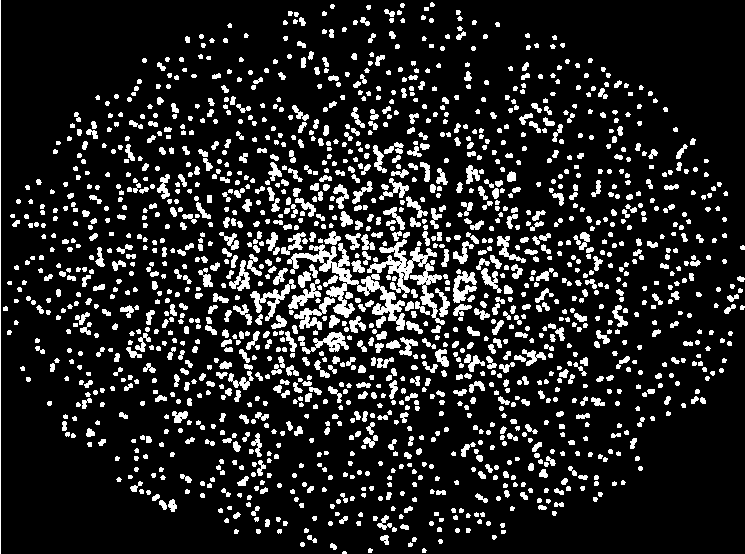
\includegraphics[width=4.1cm]{img/GCmessier_noticks_cropped.pdf}
  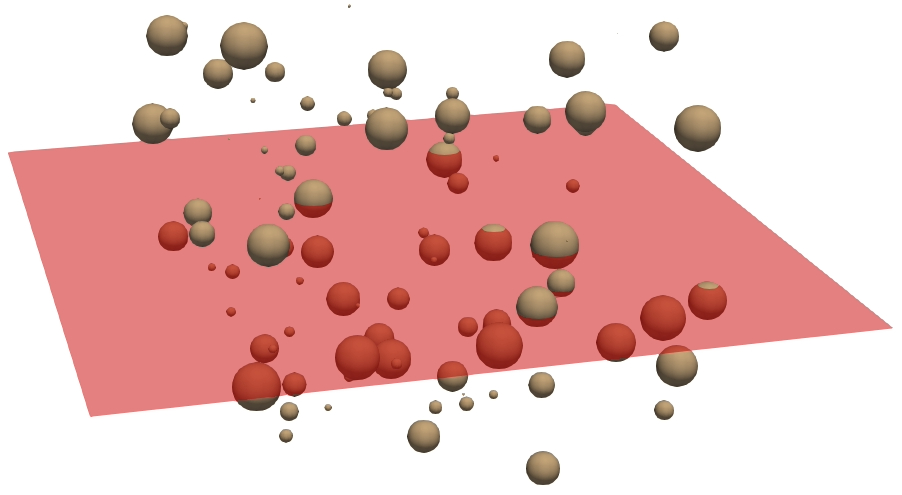
\includegraphics[width=5.1cm]{img/wicksell.jpg}
  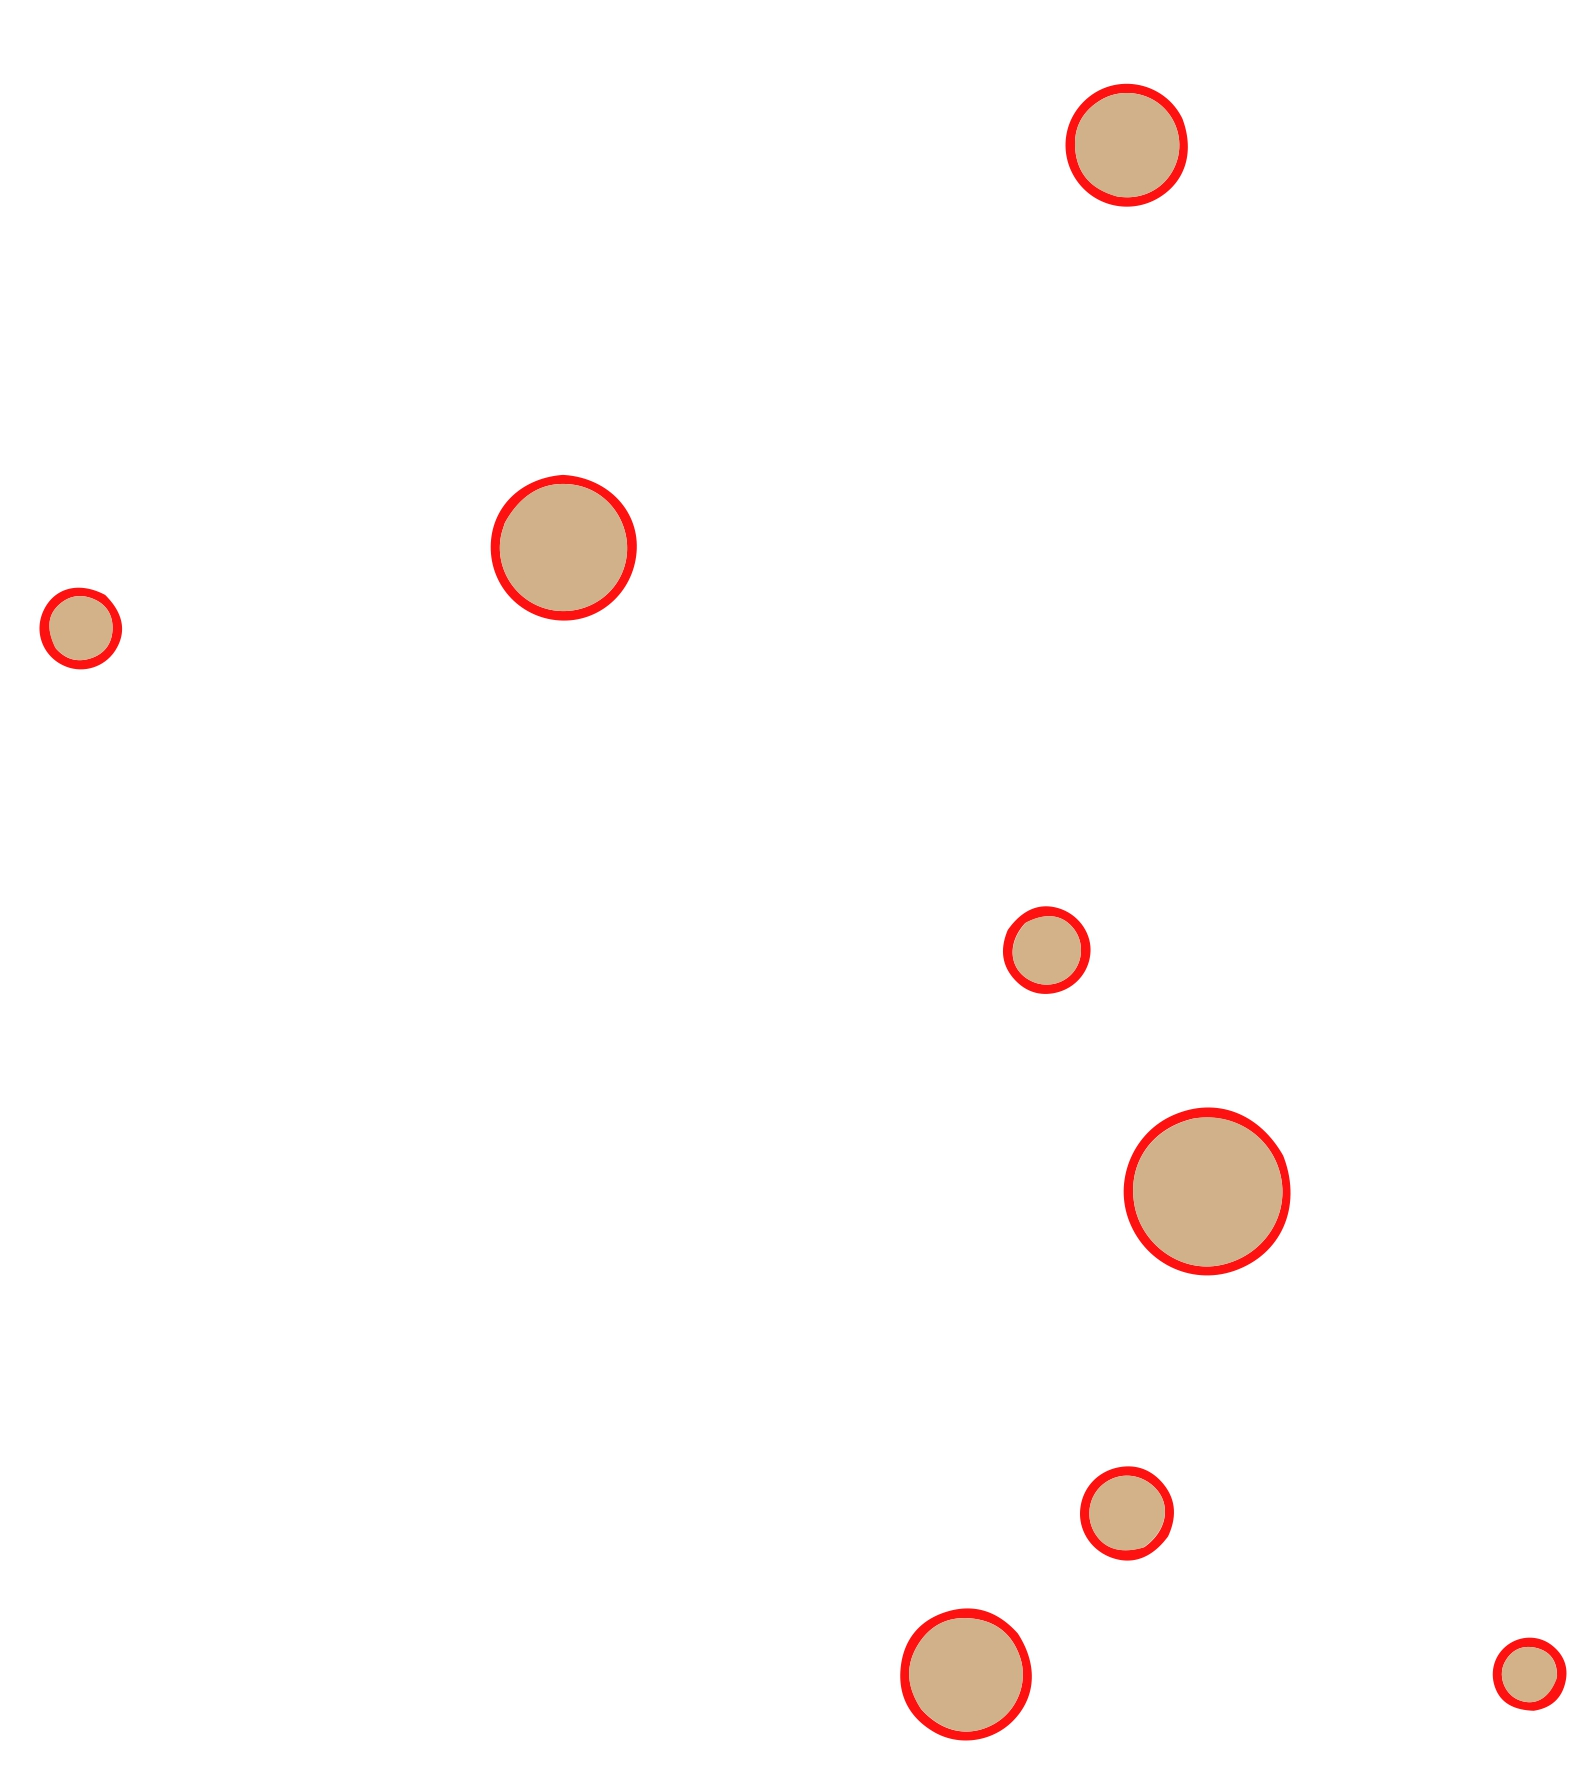
\includegraphics[width=2.7cm]{img/wick_sec_1_adobe_express_page.jpg}
  \setlength{\belowcaptionskip}{-4pt}
  \caption{Two examples of sampling in stereological inverse problems. Left panel: The Messier 4 (also designated NGC 6121) is a globular cluster in the constellation of Scorpius. Center and right panel: simulation 3D configuration with spheres and the intersecting plane in material microstructures (from \cite{27}).}\label{fig: 1 sampling}
\end{figure}

Despite their seemingly distant nature, both of these problems share a common thread: the inherent structure of an inverse problem, originally conceptualized by Wicksell (cf.\ \cite{27,1,14,15}). There, the setting of the opaque material having globular microstructure is formalized by assuming the embedded particles' radii are i.i.d.\ realization from a random variable $X^* \sim F^*$ and our observations consist of cross sections of the medium (i.e.\ "planes cutting the medium"). 

To formalize further the model note first the following two aspects: the observable radii in the cross sections cannot exceed the radii of the associated sphere; the spheres with bigger radii are more likely to be sampled. From this follows that the distribution of the squared radii of the spheres actually cut is not $F^*$ but a biased version of it; thus we write for the squared radius of the sphere actually cut: $X \sim F$. Since we assume that the samples are gathered uniformly, by Pythagoras Theorem, the observable squared circle radius $Z$ is related to $X$ via: $ Z = (1-U^2) X = Y X,$ where $U \sim U[0,1]$ and $Y \sim \operatorname{Be}(1,1/2)$. In the astronomical application, let $\mathbf{Z}= (Z_{p_1}, Z_{p_2},Z_{p_3})$ be a spherically symmetric random vector (the three-dimensional position of a star in a galaxy) of which only $(Z_{p_1}, Z_{p_2})$ can be observed. Under the assumption that the joint of $\mathbf{Z}$ is a function of the distance to the center of the galaxy, astronomers are interested in estimating the distribution of the squared distance of a star to the center of the globular cluster or galaxy $X = Z^2_{p_1}+ Z^2_{p_2}+Z^2_{p_3} \sim F$ using $Z = Z^2_{p_1}+ Z^2_{p_2} \sim G$. 

From \cite{1} and \cite{19}, it follows that both for the application in materials science and the one in astronomy, the density of the observable squared circle radii $Z \sim G$ is:
\begin{align}\label{eq: density of the observations}
g(z)=\frac{1}{2 m_0} \int_{z}^{\infty} \frac{d F^*(x)}{\sqrt{x-z}} \quad \left(= \int_{z}^{\infty} \frac{dF(x)}{2\sqrt{x^2 - xz}} \right),    
\end{align}
where $ 0 < m_0=\int_0^{\infty} \sqrt{y} \, d F^*(y) < \infty$ is the expected sphere radius under $F^*$. We can invert the above expression and obtain for $x >0$:
\begin{align*}
  & F^*(x) = 1 - \frac{V(x)}{V(0)}, \quad \quad \text{and} \quad \quad   F(x) = 1 + \frac{2}{\pi} \int_{x}^{\infty} \sqrt{s} \, dV(s) \numberthis \label{eq: solution range equation*}
\end{align*}
where, for all $x \geq 0$:
\begin{align}\label{eq: V_0 chapter2}
    V(x) \vcentcolon=\int_x^{\infty} \frac{g(z)}{\sqrt{z-x}} \: d z \quad \left(= \int_{x}^{\infty} \frac{\pi}{2 \sqrt{s}} \, dF(s)\right) 
\end{align}
and $F^*(x) = 0$ for all $x \leq 0$.  In the following sections, we will often focus on the estimation of $V$, being the common denominator for the estimation of both $F$ and $F^*$. We will also show formally how asymptotic results for the estimation of $V$ carry on to the estimation of $F^*$. Finally it is also possible to see that asymptotic results for the estimation of $V$ at $x$ carry on to the estimation of $F$ due to the following inverse formula (c.f.\ \cite{19}): 
$$
F(x) = \frac{2}{\pi} \int_0^{\infty}\sin^{-1} \left\{ \sqrt{\frac{x \wedge z}{z}} \right\} g(z)\, d z - \frac{2}{\pi} \sqrt{x} \,V(x),
$$
where the functional $\int_0^{\infty}\sin ^{-1} \sqrt{\frac{x \wedge z}{z}} g(z)\, d z$ is generally estimable at a faster rate than $V$, as its variance is finite.

\section{Adaptive and Efficient Isotonic Estimation}

Given a sample $Z_1, \ldots, Z_n$ from the density $g$ and for $\mathbb{G}_n$ the empirical distribution function based on this sample, a naive (empirical plug-in) estimator of $V$ is:
\begin{align}\label{eq: naive estimator of V chapter2}
    V_n(x) \vcentcolon=\int_x^{\infty} \frac{d\mathbb{G}_n(z)}{\sqrt{z-x}}.
\end{align}
The estimator for $F^*$ is then defined by $F^*_n(x) = 1- V_n(x)/V_n(0)$. As a function of $x$, this estimator has some undesirable properties, being non-monotone and having infinite discontinuities at a set of points becoming dense in the support of the density $g$ as $n \rightarrow \infty$. This led in \cite{1} to the definition of the so-called "isotonic inverse estimator" (IIE) $\hat{F}^*_n$ for $F^*$, which is obtained by replacing $V_n$ by its isotonic projection. This can be calculated as the right continuous derivative of the least concave majorant of the primitive function of $V_n$, which is:
$$
U_n(x)=\int_0^x V_n(y) \, dy=2 \int_0^{\infty} \sqrt{z} \, d\mathbb{G}_n(z)-2 \int_x^{\infty} \sqrt{z-x} \, d \mathbb{G}_n(z).
$$
Note that $x \mapsto U(x) = \int_{0}^x V(y) \, dy$ is a concave and increasing function on $[0,\infty)$, whereas $U_n$ is not. Taking the least concave majorant of $U_n$ on $[0,\infty)$ yields an increasing concave function. Denote by $\hat{V}_n$ the right derivative of this least concave majorant of $U_n$, and note that this will be a decreasing function on $[0,\infty)$. Then $\hat{F}^*_n$ is given by: 
\begin{align}\label{eq: isotonic estimator of F}
\hat{F}^*_n(x) := 1 - \hat{V}_n(x)/\hat{V}_n(0).
\end{align}
This estimator has the important properties of being monotone (see Figure \ref{fig: estimator performance}), right-continuous and, away from the boundary point $0$, does not depend on tuning parameters, unlike other estimators in the literature (cf.\ \cite{10}). Since $0$ is a boundary point, in the asymptotic results below $\hat{V}_n(0)$ in \eqref{eq: isotonic estimator of F} is replaced by $\hat{V}_n(x_n)$ for a sequence $x_n \downarrow 0$ (see Theorem \ref{thm: normality Holder}) and, if $F^*$ is constant around $0$, by $\hat{V}_n(y)$ for a fixed $y$ in the interior of $K_0$ (see Theorem \ref{thm: main thm iso 2}).

\begin{figure}[H]
  \vspace{-0.2cm}
  \centering
  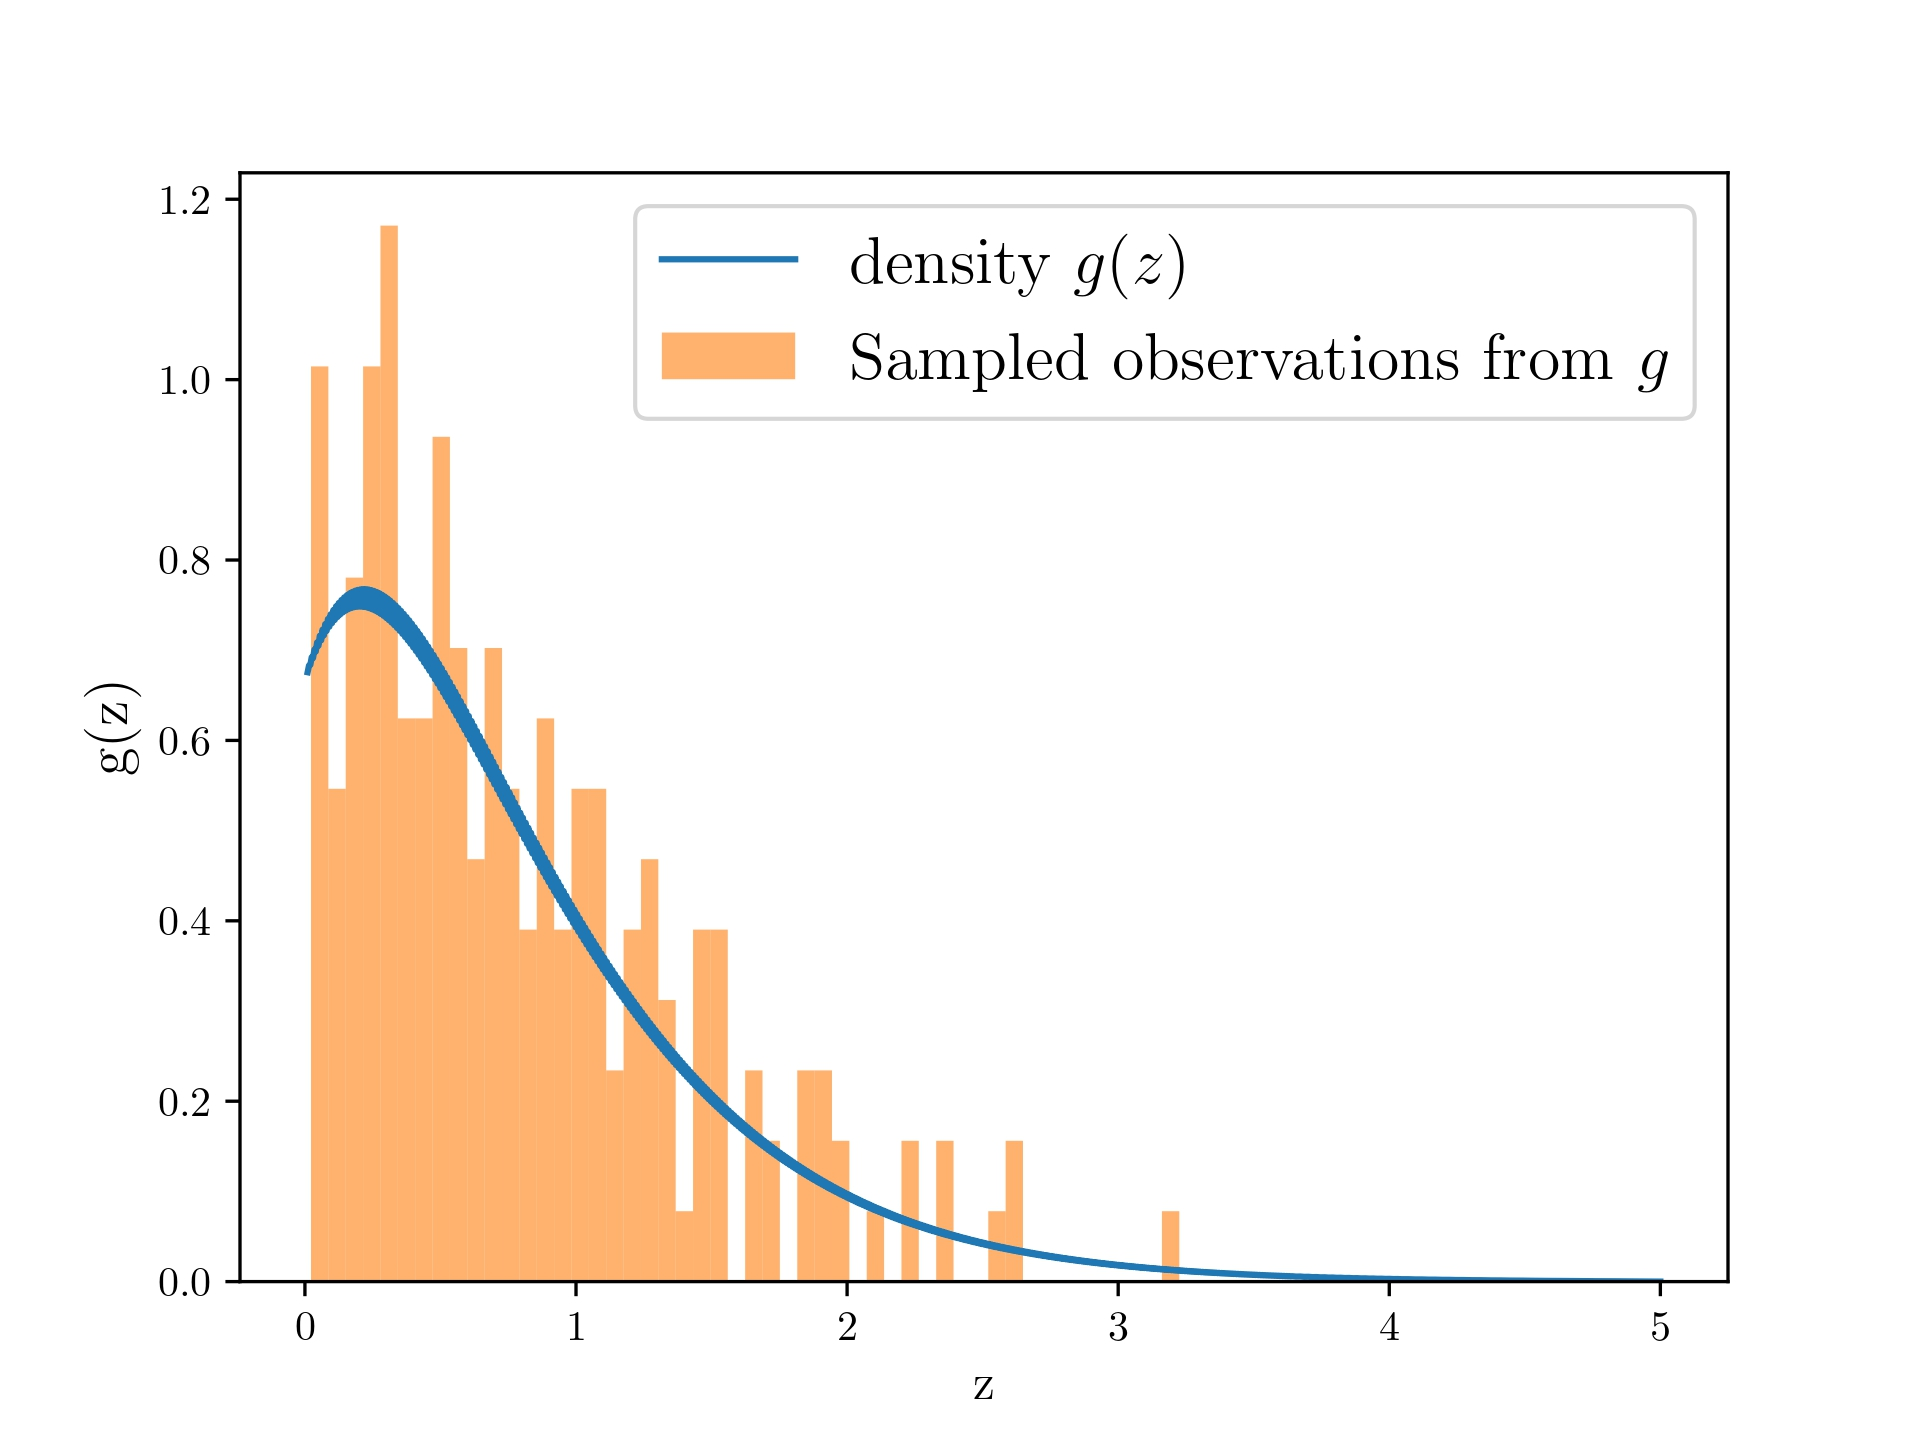
\includegraphics[width = 6cm]{img/density_new_page.jpg}
  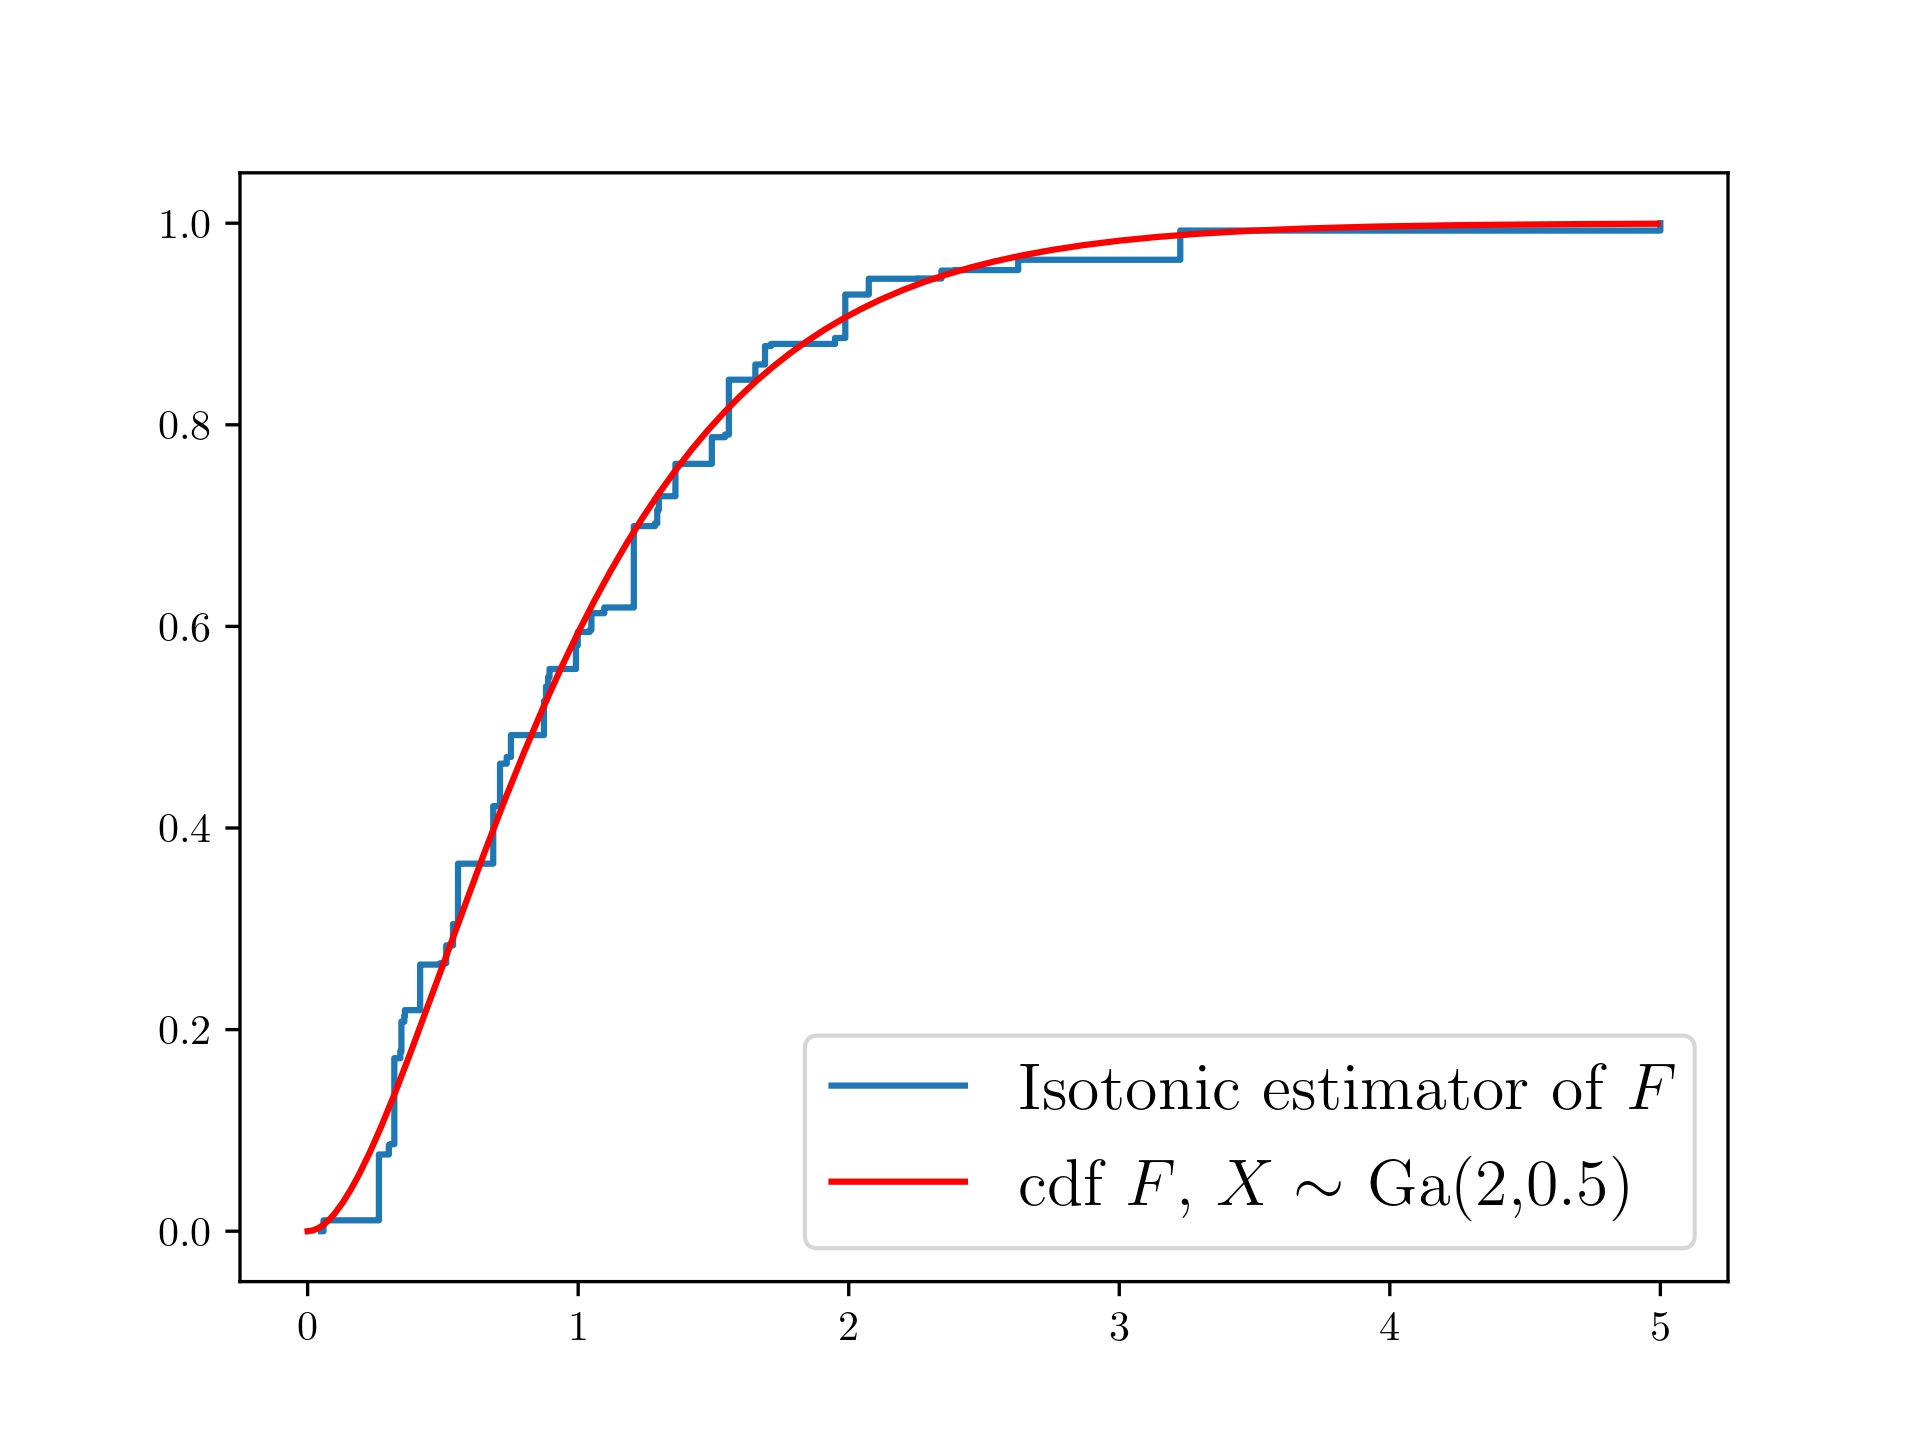
\includegraphics[width = 6cm]{img/estimator_new_page.jpg}
  \setlength{\abovecaptionskip}{-4pt}
  \setlength{\belowcaptionskip}{-8
  pt}
  \caption{200 observed draws from $g$ and isotonic estimator for $F \sim \operatorname{Ga}(2,0.5)$.}\label{fig: estimator performance}
\end{figure}

The work in this section is closely related to \cite{10} and \cite{1}. In \cite{1}, the authors observed a peculiar behavior of the isotonic estimator (IIE) compared to the naive estimator \( F^*_n(x) = 1- V_n(x)/V_n(0) \). Both estimators exhibit the same rate of estimation, \((\log{n})^{-1/2}\sqrt{n}\), and normal limiting behavior. However, the naive estimator's asymptotic variance \(\sigma^2(F^*) = \frac{4m^2_0}{\pi^2}(g(x) + g(0)(1-F^*(x))^2)\) is exactly twice that of the IIE. The authors of \cite{10} propose an explanation, showing that for \( F^* \) in the Hölder class \(\Lambda_\gamma\) with \(\gamma > \frac{1}{2}\), any efficient estimator attains the variance \(\sigma^2(F^*)/(2\gamma)\). In \cite{1}, it is assumed that \(F^*\) has a bounded density \(f\), which corresponds to \(\gamma = 1\), thus explaining the variance reduction by half.

Moreover, the authors of \cite{10} propose an estimator based on Kernel Density Estimation (KDE) that achieves the variance \(\sigma^2(F^*)/(2\gamma)\) and which is, to the best of our knowledge, the only other efficient estimator in the literature. However, the estimator they propose depends directly on the degree $\gamma$ of smoothness, which should be guesstimated before using the estimator, making it non-adaptive. Furthermore, under local conditions at $x$ and $0$ (cf. (24) and (25)), they derive an asymptotic minimax lower bound assuming $F$ is in the Hölder class $\Lambda_\gamma$, for $\gamma> \frac{1}{2}$. 

This section has two main contributions. On the one hand, we show that the IIE \(\hat{F}^*_n\) automatically adapts to the \textit{local} smoothness of \(F^*\) at \(x\), without requiring \(F^*\) to belong to a \textit{global} Hölder class. It suffices to consider the \textit{local} smoothness at points \(x\) and \(0\), measured by constants \(\gamma_x > \frac{1}{2}\) and \(\gamma_0 > \frac{1}{2}\) (see conditions \eqref{eq: condition roughness intro} and \eqref{eq: condition roughness infimum}). These can be interpreted as the tight degree of Hölder smoothness at the points $x$ and $0$. For $F^*$ with density $f$ (i.e.\ differentiable at $x$ and $0$) we retrieve the $\gamma_x = \gamma_0 = 1$ that explains the behavior observed in \cite{1}. On the other hand, we prove a lower bound on the minimax risk for any estimator sequence. The minimax theorem holds as well under local conditions of smoothness of $F^*$ around $x$ and $0$. If all conditions are met, this shows that the isotonic estimator is asymptotically efficient. No other estimator in the literature simultaneously has these properties. Consequently, the IIE emerges as the unequivocal choice, surpassing alternative estimators previously proposed in Wicksell's problem. 

First, we prove that the IIE is asymptotically normal and the smoother the cdf $F^*$ is at $x$ and $0$, the smaller the asymptotic variance automatically attained by the IIE (Theorem  \ref{thm: main thm iso 1}). Here, the smoothness of $F^*$ at a point $p$ is measured by considering constants $K_p >0$ and $\gamma_p > \frac{1}{2}$ such that:
\begin{align*}
    & \quad H_{p}(\delta ) \vcentcolon = \int_{0}^{1} \left( F^*(p+u\delta)-F^*(p) \right) \, du \sim \operatorname{sgn}(\delta) |\delta|^{\gamma_p} K_p, \quad \quad \text{as} \: \delta \rightarrow 0. \numberthis \label{eq: condition roughness intro} 
\end{align*}
Note that for $p=0$ we can only allow $\delta >0$, because $\delta <0$ would lead to $K_0 = 0$.

The adaptivity extends also to the situation where $F^*$ is constant around $x$ and $0$. Then a faster $\sqrt{n}$-rate of convergence is attained (Theorem \ref{thm: main thm iso 2}). Note that previously there were no results in the literature for nonparametric estimators that attained $\sqrt{n}$-rate in Wicksell's problem. In the case in which $F^*$ is constant only around $x$ but not around $0$, or vice versa, the rate will be again $ (\log{n})^{-1/2} \, \sqrt{n}$. We now state the first main result and its \hyperlink{proof of main thm}{proof} is given in Appendix \ref{sec: appendix chapter2}. 

\begin{theorem}\label{thm: main thm iso}
Let $F^*$ be the distribution function of the squared sphere radii and $g$ the corresponding density of the squared circle radii according to \eqref{eq: density of the observations}. Assume $\int_{0}^{\infty} y^{\frac{3}{2}} \: dF^*(y)  < \infty$ and choose $x >0$. 
\begin{thmlist}
    \item If $F^*$ satisfies condition \eqref{eq: condition roughness intro} both at $0$ and at $x$ for $\gamma_0 > \frac{1}{2}$ and $\gamma_x > \frac{1}{2}$ respectively and $g(x)<\infty$ holds true, then, as $n \rightarrow \infty$: \label{thm: main thm iso 1}
    \begin{align*}
    & \sqrt{\frac{n}{\log n}}\left( \hat{F}^*_n(x)-F^*(x)\right) \rightsquigarrow N\left(0, \frac{4m^2_0}{\pi^2} \left(\frac{g(x)}{2\gamma_x} + (1-F^*(x))^2 \frac{g(0)}{2\gamma_0} \right)\right).
    \end{align*} 
    \item If $F^*$ is constant around $x$ and $0$, with $K_x$ and $K_0$ the biggest compact intervals in $[0,\infty)$ that contain $x$ and $0$, respectively, so that $F^*$ is constant, on $K_x$ and $K_0$, with $K_x \cap K_0 = \emptyset$ and $x$ in the interior of $K_x$, then, for $\hat{F}^*_n(x) := 1 - \hat{V}_n(x)/\hat{V}_n(y)$ with $y$ a fixed point in the interior of $K_0$, as $n \rightarrow \infty$: \label{thm: main thm iso 2}
    \begin{align*}
        \sqrt{n} \left( \hat{F}^*_n(x) - F^*(x) \right) \rightsquigarrow \frac{2m_0}{\pi} \Big(L_x+ (1-F^*(x))L_0 \Big), 
    \end{align*}
    where, for any $a,b \in \mathbb{R}$, the joint distribution of $L_x$ and $L_0$ is given by:
    \begin{align*}
        \pb \left( L_x \leq a, L_0 \leq b \right) = \pb \, \bigg( \argmax_{s \in K_x} \left\{ \mathbb{Z}_x(s) - a s\right\} \leq x, \argmax_{s \in K_0} \left\{ \mathbb{Z}_y(s) - b s\right\} \leq y \bigg).
    \end{align*}
    Here $\mathbb{Z}_p(s) = \mathbb{Z}(s) - \mathbb{Z}(p),$ for $s \geq 0$ and $p \in \{x,y\}$. $\mathbb{Z}$ is a continuous centered Gaussian Process with covariance structure given by:
    \begin{align}\label{eq: covariance gauss process}
        \mathrm{Cov} \left( \mathbb{Z}(t),\mathbb{Z}(s) \right) = \mathrm{Cov} \Big( 2 \big( \sqrt{\smash[b]{Z}} - \sqrt{\smash[b]{(Z_t)_{+}}} \big), 2 \big( \sqrt{\smash[b]{Z}} - \sqrt{\smash[b]{(Z_s)_{+}}} \big) \Big),
    \end{align}
    where $Z_t = Z - t$ and $Z_s = Z - s$.
\end{thmlist}
\end{theorem}
  
The second main result of this section consists of showing that the IIE is asymptotically efficient in this setting, i.e.\ the attained asymptotic variance is the smallest attainable. This kind of result is obtained by proving a minimax lower bound for any estimator sequence estimating $F^*(x)$. Here we give a weaker (but perhaps more insightful) version of this result and its \hyperlink{proof of thm 2}{proof} is given in Appendix \ref{sec: appendix chapter2}. 

\begin{theorem}\label{thm: LAM weaker}
    Let the conditions of Theorem \ref{thm: main thm iso 1} hold, assume that $F^*$ for such $\gamma_0, \gamma_x$ satisfies \eqref{eq: condition roughness infimum} and that $g$ is continuous at $x$ and $0$. Let $\ell$ be a bowl-shaped loss function, i.e., $\ell$ is non-negative, symmetric and subconvex, then for any estimator sequence $\left( F^*_n(x)\right)_{n \in \mathbb{N}}$:
    \begin{align}\label{eq: LAM simplified}
        \lim_{\delta \downarrow 0} \: \: \liminf_{n \rightarrow \infty} \, \sup_{\| F^{\prime } - F^* \|_{\infty} < \delta} \, \ex_{\scriptscriptstyle{G_{{\scaleto{F^{\prime}}{3.7pt}}}}} \, \ell\left(\sqrt{\frac{n}{\log{n}}}\left(F^*_n(x)- F^{\prime}(x)\right)\right)  \geq \ex \ell(L),
    \end{align}
where $L$ possesses the normal distribution in Theorem \ref{thm: main thm iso 1}. $G_{F^\prime}$ is the probability measure associated to the density $g$ in \eqref{eq: density of the observations} with $F^*$ replaced by $F^\prime$.
\end{theorem}
Combining the above results shows that the IIE is an easy-to-compute, adaptive (at $x$), and efficient estimator for $F^*$.

\subsection{Asymptotics of the Isotonic Inverse Estimator}

In this subsection, we prove two main theorems that will imply Theorem \ref{thm: main thm iso}. In order to prove Theorem \ref{thm: main thm iso 1}, it is enough to look at the behavior of $\hat{V}_n(x)$ and then apply the same result also to $\hat{V}_n(0)$. We now state the conditions needed for Theorem \ref{thm: main thm iso} and \ref{thm: normality Holder}. First, a natural assumption is a moment constraint for $Z$, which can be translated into a moment condition on $X^*$ (for $0 < m_0 < \infty$): 
\begin{align*}
    \quad \int_{0}^{\infty} z \, g(z) \, dz = \frac{2}{3m_0} \int_{0}^{\infty} y^{\frac{3}{2}} \: dF^*(y)  < \infty. \numberthis \label{eq: finite first moment chapter2}
\end{align*}
Additionally, for $x \geq 0$, we need our version of $g$ to be well defined, i.e.:
\begin{align*}
    \frac{1}{2m_0}\int_{x}^{\infty} \frac{dF^*(s)}{\sqrt{s - x}}  < \infty. \numberthis \label{eq: condition finite g at x chapter2}
\end{align*}
Furthermore, we measure the smoothness of $F^*$ at $x$; $\exists$ $K >0$ and $\gamma_x > \frac{1}{2}$ such that \eqref{eq: condition roughness intro} is satisfied. 

Before proving Theorem \ref{thm: main thm iso 1}, we show that condition \eqref{eq: condition roughness intro} entails the local smoothness of the distribution function $F$ by looking at the following examples \ref{example: cdf holder} and \ref{example: cdf discrete holder} below.
\begin{example}\label{example: cdf holder}
For $\gamma_x> \frac{1}{2}$ consider the class of distribution functions locally behaved as follows. Let $F^*$ be so that there exists a neighborhood $U_x$ of $x>0$ and some $K>0$:
\begin{align*}
    F^*(u) = \begin{cases}
        F^*(x) + K(u-x)^{\gamma_x}, \quad \quad \text{for} \: u \geq x, \: u \in U_x \\
        F^*(x) - K(x-u)^{\gamma_x}, \quad \quad \text{for} \: u < x, \: u \in U_x
    \end{cases}
\end{align*}
One can think of such distribution functions as tightly Hölder smooth of degree $\gamma_x$ at the point $x$. This class is of particular importance because it illustrates what type of functions we are thinking of when we derive results under smoothness conditions at the point $x$ and 0. Such functions satisfy both conditions \eqref{eq: condition roughness intro} and \eqref{eq: condition roughness 2}. Condition \eqref{eq: condition roughness 2} follows immediately. For condition \eqref{eq: condition roughness intro} note that as $|\delta| \downarrow 0$, small enough so that $[x-|\delta|, x + |\delta|] \subset U_x$:
\begin{align*}
    H_x(\delta) = \int_{0}^{1} \left( F^*(x+u\delta )-F^*(x) \right) \, du =  \operatorname{sgn}(\delta) |\delta|^{\gamma_x} K \int_{0}^{1} u^{\gamma_x} \, du + o(\delta).
\end{align*}
\end{example}

\begin{example}\label{example: cdf discrete holder}
For any $x >0$, let $\mu_x$ be the discrete probability measure given by:
\begin{align*}
    \mu_x = \frac{1}{2} \sum_{i=1}^{\infty} p_i \left( \delta_{x+t_i} + \delta_{x-t_i}\right) ,
\end{align*}
for sequences $p_i$ of probability weights and $t_i \downarrow 0$. In particular set: $p_i = \frac{6}{\pi^2} i^{-2}$ and $t_i = i^{-\frac{1}{\gamma_x}}$ where $\gamma_x> 1/2$ and $\delta_x(\cdot)$ indicates the Dirac measure at $x$. Denote by $F^*$ the associated cdf, so that, because $\gamma_x> 1/2$, we have:
\begin{align*}
    \int_{x}^{\infty} \frac{dF^*(s)}{\sqrt{s-x}} = \frac{3}{\pi^2} \sum_{i=1}^{\infty} \frac{1}{i^2}\frac{1}{\sqrt{t_i}} = \frac{3}{\pi^2} \sum_{i=1}^{\infty} \frac{1}{i^{2- \frac{1}{2\gamma_x}}} < \infty.
\end{align*}
Moreover, we have for $\delta \downarrow 0$ (similar reasonings hold also for a generic sequence $|\delta| \downarrow 0$, we consider $\delta >0$ for simplicity):
\begin{align*}
    H_x(\delta) = \int_{0}^{1} \left( F^*(x+u\delta) - F^*(x) \right) \, du = \sum_i \frac{p_i}{2} \int_{0}^{1} \ind_{t_i \leq u \delta} \, du = \sum_i \frac{p_i (\delta - t_i)_{+}}{2\delta},
\end{align*}
which means $t_i< \delta$, thus $i > \frac{1}{\delta^{\gamma_x}}$. Therefore $H_x(\delta) = \sum_{i > 1/\delta^{\gamma_x}} \frac{p_i(\delta - i^{-1/\gamma_x})}{2\delta}$. Now we prove the following fact, as $\delta \downarrow 0$ and $k \geq 2$:
\begin{align*}
    \frac{1}{(\delta^{\gamma_x})^{k-1}} \sum_{i> \frac{1}{\delta^{\gamma_x}}} \frac{1}{i^k} \stackrel{\delta \downarrow 0}{\longrightarrow} \frac{1}{k-1}
\end{align*}
This follows directly from the fact that for $\alpha \rightarrow \infty$ (e.g.\ $\alpha = 1/\delta^{\gamma_x}$) we have:
\begin{align*}
    \frac{1}{k-1} \frac{1}{(\alpha+1)^{k-1}} = \int_{\alpha + 1}^{\infty} \frac{1}{x^k} dx \leq \sum_{i > \alpha} \frac{1}{i^k} \leq \int_{\alpha-1}^{\infty} \frac{1}{x^k} dx = \frac{1}{k-1} \frac{1}{(\alpha - 1)^{k-1}}
\end{align*}
Moreover $(\alpha/(\alpha \pm 1))^{k-1} \rightarrow 1$. Therefore as $\delta \downarrow 0$ we have:
\begin{align*}
    H_x(\delta) = \frac{6}{\pi^2} \left( \sum_{i > 1/ \delta^{\gamma_x}} \frac{1}{i^2} - \frac{1}{\delta} \sum_{i > 1/ \delta^{\gamma_x}} \frac{1}{i^{2+ \frac{1}{\gamma_x}}}\right) \sim  \frac{6}{\pi^2 (1+\gamma)} \delta^{\gamma_x}.
\end{align*}
This demonstrates that the required condition for Theorem \ref{thm: normality Holder} can also be satisfied for a discrete cumulative distribution function.
\end{example}

\begin{remark}
    Example \ref{example: cdf holder} shows that \textit{tight} Hölder smoothness of degree $\gamma_x$ at the point $x$ implies \eqref{eq: condition roughness intro}. The implication in the other direction is not true as it is shown by Example \ref{example: cdf discrete holder}, where a distribution that is not Hölder continuous at $x$ satisfies \eqref{eq: condition roughness intro}. This example also shows that \eqref{eq: condition roughness intro} does not imply Hölder continuity of $F^*$ at $x$ (i.e.\ $|F^*(x+\delta) - F^*(x)| = O(|\delta|^{\gamma_x})$ as $\delta \rightarrow 0$). The condition $|F^*(x+\delta) - F^*(x)| = O(|\delta|^{\gamma_x})$ as $\delta \rightarrow 0$ is also not sufficient for Theorem \ref{thm: normality Holder} because $|F^*(x+\delta) - F^*(x)| = O(|\delta|^{\gamma_x})$ only gives information about the upper bound of the difference, but not about the lower bound, which is also needed to be tight Hölder of degree $\gamma_x$, as can be seen by inspection of the proof of Theorem \ref{thm: normality Holder}.
\end{remark}

\begin{theorem}\label{thm: normality Holder}
Let $x \geq 0$, suppose that\eqref{eq: condition roughness intro}, \eqref{eq: finite first moment chapter2}, and\eqref{eq: condition finite g at x chapter2} hold true and $g(x)$ is given by \eqref{eq: density of the observations}. Then:
\begin{align*}
    \sqrt{\frac{n}{\log n}}\left(\hat{V}_n(x)-V(x)\right) \rightsquigarrow N\left(0, \frac{1}{2 \gamma_x} g(x)\right) \quad \text { as } n \rightarrow \infty \text {,}
\end{align*}
where, for $x=0$, we define $\hat{V}_n(0) := \hat{V}_n(x_n)$ for a sequence $x_n = o\big((n/\log n)^{-1/(2\gamma_0)}\big)$ such that $\log(1/x_n) \sim \frac{1}{2\gamma_0}\log n$ (e.g.\ $x_n = (n/\log n)^{-1/(2\gamma_0)}/\log n$).
\end{theorem}
\begin{proof}
We generalize the proof of \cite{1}, for $\gamma_x\neq 1$.

First note that \eqref{eq: condition roughness intro}, implies that $F^*$ is not constant in a neighborhood of $x$ (c.f.\ Lemma \ref{lemma: finite g if rough 2}). 
Fix $x \geq 0$ such that $x$ satisfies the conditions stated above. Define, for $a>0$, the process $T_n$ as follows:
$$
T_n(a)=\inf \left\{t \geq 0: U_n(t)-a t \text { is maximal }\right\}.
$$


The relation between $T_n$ and $\hat{V}_n$ is given by the switch relation (see \cite{2}):
\begin{align}\label{eq: switch relation}
T_n(a) \leq t \quad \Leftrightarrow \quad \hat{V}_n(t) \leq a .
\end{align}
From this relation (Lemma 3.2, \cite{2}), it follows that for each vanishing sequence $\left(\delta_n\right)$ of positive numbers, for $a\in \mathbb{R}$, for $\delta^*_n = \delta_n^{1/\gamma_x}$ ($\gamma_x$ as in \eqref{eq: condition roughness intro}), and all $n$ sufficiently large:
\begin{align*}
\delta_n^{-1}\left(\hat{V}_n(x)-V(x)\right) \leq a \: \: \: \: \: &\Leftrightarrow \: \: \: \: \: \delta_n^{-1}\left(T_n\left(a_0+\delta_n a\right)-x\right) \leq 0 \: \: \: \: \: \\
&\Leftrightarrow \: \: \: \: \: (\delta^*_n)^{-1}\left(T_n\left(a_0+\delta_n a\right)-x\right) \leq 0. 
\end{align*}
We aim to study the probability of the event on the left-hand side. We write $a_0$ for $V(x)$, which is fixed. The introduction of $\delta^*_n = \delta_n^{1/\gamma_x}$ is one of the main steps that differentiates the current proof from the one in \cite{1}. Now denote by:
$$
I_x := \begin{cases}{[0, \infty),} & \text { if } x=0 \\ \mathbb{R}, & \text { if } x>0\end{cases}
$$
\color{black} Define the localized process $\tilde{Z}_n$ in $C\left(I_x\right)$, the space of continuous functions on $I_x$, as follows (recall $a_0 = V(x)$):
$$
\tilde{Z}_n(t)=\delta_n^{-1} (\delta^*_n)^{-1} \left[U_n\left(x+\delta^*_n t\right)-U_n(x)-a_0 \delta^*_n t\right] .
$$
For each fixed $a \in \mathbb{R}$ we can, for all $n$ sufficiently large, write 
$$
\begin{aligned}
& (\delta^*_n)^{-1}\left(T_n\left(a_0+\delta_n a\right)-x\right) \\
&\quad = (\delta^*_n)^{-1} \big(\operatorname { i n f } \big\{x+t \geq 0: U_n(x+t)-a_0 x +\\
&\quad \quad \quad \quad \quad \quad \quad \quad \quad \quad \quad \quad -a_0 t-\delta_n a x-\delta_n a t \text { is maximal }\big\}-x\big) \\
&\quad = (\delta_n^*)^{-1} \inf \left\{t \geq-x: U_n(x+t)-U_n(x)-a_0 t-\delta_n a t \text { is maximal }\right\} \\
&\quad = \inf \left\{t \geq-(\delta^*_n)^{-1} x: U_n\left(x+\delta^*_n t\right)-U_n(x)-a_0 \delta^*_n t-\delta_n \delta^*_n a t \text { is maximal }\right\} \\
&\quad = \inf \left\{t \geq-(\delta^*_n)^{-1} x: \tilde{Z}_n(t)-a t \text { is maximal }\right\} ,
\end{aligned}
$$
where we use that the location of a maximum of a function is equivariant under translations and invariant under multiplication by a positive number and addition of a constant. Thus we analyze the asymptotic behavior of the process:
\begin{align*}
    \tilde{Z}_n(t)-a t =& \: \delta_n^{-1} ( \delta^*_n)^{-1} \left\{U_n\left(x+\delta^*_n t\right)-U_n(x)- U\left(x+\delta^*_n t\right)+U(x)\right\} \color{black}+ \numberthis \label{eq: rewrite Z tilde 1}\\ 
    &+ \delta_n^{-1} ( \delta^*_n)^{-1}  \left\{ U\left(x+\delta^*_n t\right)-U(x)-V(x)\delta^*_n t \right\} - at. \numberthis \label{eq: rewrite Z tilde}
\end{align*}
We will now analyze the behavior of the stochastic and deterministic terms \eqref{eq: rewrite Z tilde 1} and \eqref{eq: rewrite Z tilde} separately. Let us start with \eqref{eq: rewrite Z tilde}. The Taylor expansion of $U$ with integral form of the remainder yields:
\begin{align*}
    U(x + \delta^*_n t) - U(x) - V(x) \delta^*_n t &= \delta^*_n t \int_{0}^{1} V(x + u \delta^*_n t) - V(x) \, du \\
    &= -\frac{\delta^*_n t \pi}{2 m_0} \int_{0}^{1} F^*(x + u \delta^*_n t) - F^*(x) \, du.
\end{align*}
When we look at the limit of $\tilde{Z}_n(t) - at$ we multiply the above expression by $ \delta_n^{-1} (\delta^*_n)^{-1}= (\delta^*_n)^{-\gamma_x- 1}$. Therefore we have to look at the limit behavior of:
\begin{align}\label{eq: reasoning asympt holder}
 - (\delta^*_n)^{-\gamma_x- 1} \frac{\delta^*_n t \pi}{2 m_0} \int_{0}^{1} F^*(x + u \delta^*_n t) - F^*(x) \, du = -\frac{ |t|^{\gamma_x+ 1} \pi}{2 m_0} (K_x + o(1)),
\end{align}
where we use assumption \eqref{eq: condition roughness intro}. 

Now we consider \eqref{eq: rewrite Z tilde 1}. Defining the processes $\left(Z_n\right)$ in $C\left(I_x\right)$ as
\begin{align*}
Z_n(t) &= \delta_n^{-1} ( \delta^*_n)^{-1} \left\{U_n\left(x+\delta^*_n t\right)-U_n(x)- U\left(x+\delta^*_n t\right)+U(x)\right\} \numberthis \label{eq: Z_n(1)} \\
&=2 \delta_n^{-1} (\delta^*_n)^{-1} \int\left\{\sqrt{z-x} \ind_{[x, \infty)}(z)-\sqrt{z-x-\delta^*_n t} \ind_{\left[x+\delta^*_n t, \infty\right)}(z)\right\} \, d\left(\mathbb{G}_n-G\right)(z)
\end{align*}
we will now establish convergence in distribution of the process $Z_n$. In order to do so, we need that $g(x) < \infty$. This follows directly from \eqref{eq: condition finite g at x chapter2}. Moreover, we need the asymptotic covariance structure of the process $Z_n$, which is given by:
\begin{align}\label{eq: covariance structure final}
\operatorname{Cov}\left(Z_n(s), Z_n(t)\right)=\frac{1}{2 \gamma_x} g(x) s t\left(1-\frac{\log \log n}{\log n}\right)+O\left(\frac{1}{\log n}\right) \text {, }
\end{align}
for each fixed $s, t \in I_x$, provided that $\delta_n=n^{-1 / 2} \sqrt{\log n}$.
Therefore, using \eqref{eq: covariance structure final} and the Lindeberg-Feller Central Limit theorem we have that: 
\begin{align}\label{eq: marginal convergence chapter2}
    Z_n(1) \rightsquigarrow N(0,g(x)/(2\gamma_x)),
\end{align} 
(the \hyperlink{proof of lemma 1}{proof} of \eqref{eq: covariance structure final} and the \hyperlink{proof of lemma 2}{proof} of \eqref{eq: marginal convergence chapter2} are provided in Appendix \ref{sec: appendix chapter2}). On the other hand, by Chebyshev's inequality and \eqref{eq: covariance structure final}, we have, $\forall \: \varepsilon >0$:
\begin{align*}
    \pb\left( | Z_n (t) - t Z_n (1) | > \varepsilon \right) \leq &\frac{\mathrm{Var} ( Z_n (t) - t Z_n (1))}{\varepsilon^2} \rightarrow 0.
\end{align*}
Therefore, the finite-dimensional distributions of $Z_n$ converge weakly to the finite-dimensional distributions of the process: $ Z(t) = tX,$ in $C(I_x)$, where $X \sim N(0,g(x)/(2\gamma_x))$. We now need a stochastic equicontinuity condition to apply Theorem 2.3 from \cite{12}. Take the class of functions for $\varepsilon >0, \: M>0$:  
\begin{align*}
\mathscr{F}_{n, \varepsilon}^M=\big\{\sqrt{z-x-\delta^*_n t} & \ind_{\left[x+\delta^*_n t, \infty\right)}(z)-\sqrt{z-x-\delta^*_n s} \ind_{\left[x+\delta^*_n s, \infty\right)}(z) :  \numberthis \label{eq: class of functions chapter2} \\
&: \: s, t \in I_x,|s-t|<\varepsilon, \max (|s|,|t|)<M\big\}.
\end{align*}
This class has square integrable natural envelope $H_\varepsilon $ that satisfies for all $\varepsilon>0$ small (cf.\ Lemma \ref{lemma: variance without assum. g}): $\int H^2_{\varepsilon} (z) g (z) dz \leq g(x + \delta^*_n s \wedge t) \left( \varepsilon \delta^*_n\right)^2 \log{\frac{1}{(\varepsilon \delta^*_n)^2}}$ (as proved in Lemma \ref{lemma: conv weak argmax} this class of functions is also VC).
Therefore, by using maximal inequality 3.1 (ii) from 
\cite{12} we obtain:
\begin{align*}
    &\limsup_{n \rightarrow \infty}\pb \left\{ \sup_{\mathscr{F}_{n, \varepsilon}^M} |Z_n(s) - Z_n(t)| > \eta \right\} \leq \limsup_{n \rightarrow \infty} \frac{\ex \sup_{\mathscr{F}_{n, \varepsilon}^M} |Z_n(s) - Z_n(t)|^2 }{\eta^2} \\
    &\leq \limsup_{n \rightarrow \infty} \, \frac{J(1)^2 g(x + \delta^*_n s \wedge t)}{(\delta^*_n)^2 \log{n}} (\varepsilon \delta^*_n)^2 \log{(\varepsilon \delta^*_n)^{-2}} =  J(1)^2 \gamma_x^{-1} \eta^{-2} g(x) \varepsilon^2 \stackrel{\varepsilon \rightarrow 0}{\longrightarrow} 0.
\end{align*}
where the reason why the uniform entropy integral is finite is as in the proof of Lemma \ref{lemma: conv weak argmax}.
The stochastic equicontinuity condition, together with the convergence in distribution of the finite-dimensional distributions, implies convergence in distribution of $Z_n$ to $Z$ in $(C(I_x),d)$ where $d$ is the metric of uniform convergence on compacta. Next, we need the stochastic boundedness of the sequence $T_n$ given below in \eqref{eq: stochastic boundedness seq argmax} (the \hyperlink{proof of lemma 3}{proof} of which is given in Appendix \ref{sec: appendix chapter2}). For $a_0 = V(x)$ and $n \rightarrow \infty$:
\begin{align}\label{eq: stochastic boundedness seq argmax}
T_n\left(a_0 + \delta_n a \right)=V^{-1}\left(a_0\right)+O_p\left(\delta^*_n\right).
\end{align}
One can now apply Theorem 2.7 from \cite{12} to the process $\tilde{Z}_n$. 
\begin{align}\label{eq: convergence argmax}
(\delta^*_n)^{-1}\left(T_n\left(a_0+\delta_n a\right)-x\right) & \rightsquigarrow \underset{t \in I_x}{\arg \max }\left\{t X-\frac{|t|^{\gamma_x+ 1} \pi}{2 m_0} K_x  -a t \right\}. 
\end{align}
But it is immediate to see that, almost surely (Lemma~\ref{lem: continuity argmax holder}):
\begin{align}\label{eq: iff relation argmax}
    \underset{t \in I_x}{\arg \max }\left\{t X-\frac{|t|^{\gamma_x+ 1} \pi}{2 m_0} K_x  -a t \right\} \leq 0 \: \: \: \: \iff \: \: \: \: X \leq a.
\end{align}
Hence, using the two relations above:
\begin{align*}
&\pb\left\{\delta_n^{-1}\left(\hat{V}_n(x)-V(x)\right) \leq a\right\}=\pb\left\{(\delta^*_n)^{-1}\left(T_n\left(a_0+\delta_n a\right)-x\right) \leq 0\right\} \stackrel{n \rightarrow \infty}{\longrightarrow} \\
& \quad \stackrel{\eqref{eq: convergence argmax}}{\longrightarrow} \pb \left\{ \underset{t \in I_x}{\arg \max }\left\{t X-\frac{|t|^{\gamma_x+ 1} \pi}{2 m_0} K_x  -a t \right\} \leq 0 \right\} \stackrel{\eqref{eq: iff relation argmax} }{=} \pb\{ X \leq a\},
\end{align*}
where the convergence holds because, for $x>0$, $0$ is a continuity point of the limit distribution in \eqref{eq: convergence argmax} (Lemma~\ref{lem: continuity argmax holder}). This proves the theorem for $x>0$.

For $x=0$ since $I_0=[0,\infty)$, the limit in \eqref{eq: convergence argmax} has an atom at $0$ of mass $\pb\{X \leq a\}$. This is why $\hat{V}_n$ is evaluated at $x_n$. Write $\hat{s}_n := (\delta^*_n)^{-1} T_n(a_0+\delta_n a)$ and $\kappa_n := x_n/\delta^*_n$, so that $\kappa_n \rightarrow 0$ and $\log(1/\kappa_n) = o(\log n)$ by the assumptions on $x_n$. By the switch relation \eqref{eq: switch relation}:
\begin{align*}
\pb\left\{\delta_n^{-1}\left(\hat{V}_n(0)-V(0)\right) \leq a\right\} = \pb\left\{\hat{V}_n(x_n) \leq a_0+\delta_n a\right\} = \pb\left\{T_n(a_0+\delta_n a) \leq x_n\right\} = \pb\left\{\hat{s}_n \leq \kappa_n\right\},
\end{align*}
so it suffices to show that $\pb\{\hat{s}_n \leq \kappa_n\} \rightarrow \pb\{X \leq a\}$. At $x=0$ the limit in \eqref{eq: convergence argmax} is, with $c := \pi K_0/(2m_0)$:
\begin{align*}
\hat{s} := \underset{t \geq 0}{\arg\max}\left\{tX - c\, t^{\gamma_0+1} - at\right\} = \left(\frac{(X-a)_+}{c(1+\gamma_0)}\right)^{1/\gamma_0}.
\end{align*}
Fix $\varepsilon>0$. For $n$ large we have $\kappa_n \leq \varepsilon$ and, since $[0,\varepsilon]$ is closed in $I_0$, the portmanteau lemma gives:
\begin{align*}
\limsup_{n \rightarrow \infty} \pb\left\{\hat{s}_n \leq \kappa_n\right\} \leq \limsup_{n \rightarrow \infty} \pb\left\{\hat{s}_n \leq \varepsilon\right\} \leq \pb\left\{\hat{s} \leq \varepsilon\right\} = \pb\left\{X \leq a + c(1+\gamma_0)\varepsilon^{\gamma_0}\right\},
\end{align*}
which tends to $\pb\{X \leq a\}$ as $\varepsilon \rightarrow 0$. For the lower bound fix $M \geq 1$ and $\eta>0$. Since $F^*$ is nondecreasing, the term in \eqref{eq: rewrite Z tilde} is at most $-at$, that is, $\tilde{Z}_n(t) \leq Z_n(t)$ for $t \geq 0$. We claim that:
\begin{align*}
\left\{Z_n(1) \leq a-\eta\right\} \cap \left\{\sup_{\kappa_n < t \leq M}\left|\frac{Z_n(t)}{t}-Z_n(1)\right| \leq \eta\right\} \cap \left\{\hat{s}_n \leq M\right\} \subseteq \left\{\hat{s}_n \leq \kappa_n\right\}.
\end{align*}
Indeed, on the event on the left-hand side we have $Z_n(t)/t \leq a$ for all $t \in (\kappa_n, M]$, and therefore
\begin{align*}
\tilde{Z}_n(t) - at \leq Z_n(t) - at \leq 0 = \tilde{Z}_n(0) \quad \text{for all } t \in (\kappa_n, M].
\end{align*}
So no point of $(\kappa_n, M]$ can be the smallest maximizer of $\tilde{Z}_n(t)-at$ (otherwise $0$ would be a maximizer smaller than it), and since $\hat{s}_n \leq M$ we get $\hat{s}_n \leq \kappa_n$. Hence:
\begin{align*}
\pb\left\{\hat{s}_n \leq \kappa_n\right\} \geq \pb\left\{Z_n(1) \leq a-\eta\right\} - \pb\left\{\sup_{\kappa_n < t \leq M}\left|\frac{Z_n(t)}{t}-Z_n(1)\right| > \eta\right\} - \pb\left\{\hat{s}_n > M\right\}.
\end{align*}
By \eqref{eq: marginal convergence chapter2} the first term converges to $\pb\{X \leq a-\eta\}$, and the second term converges to zero by Lemma~\ref{lemma: uniform collapse} (see Appendix \ref{sec: appendix chapter2}). By \eqref{eq: stochastic boundedness seq argmax} with $x=0$, $\hat{s}_n = O_p(1)$, so the last term is arbitrarily small for $M$ large, uniformly in $n$. Letting $n \rightarrow \infty$, then $M \rightarrow \infty$ and $\eta \rightarrow 0$, we obtain $\liminf_{n} \pb\{\hat{s}_n \leq \kappa_n\} \geq \pb\{X \leq a\}$, which concludes the proof for $x=0$.
\end{proof}

\begin{example}\label{example: holder + local behavior}
As in \cite{10}, it is possible to conduct the analysis in accordance with the global smoothness properties of the underlying distribution function $F^*$. Consider, for arbitrary $\gamma=\alpha+\beta, \alpha=0,1, \ldots, 0<\beta \leq 1$, the Hölder class $C^{\gamma}$ of functions $f(y), y \geq 0$ having finite norm:
\begin{align}\label{eq: holder norm definition}
\|f\|_\gamma=\sup _{y \geq 0}|f(y)|+\sup _{x, y \geq 0} \frac{\left|f^{(\alpha)}(x)-f^{(\alpha)}(y)\right|}{|x-y|^\beta}.
\end{align}
Then assume $F \in C^{\gamma}$ for $\gamma > \frac{1}{2}$. Moreover, assume:
\begin{align}\label{eq: condition roughness 2}
    \lim_{t \rightarrow 0} \frac{|F^*(x+t)-F^*(x)|}{|t|^{\gamma}} = K > 0.
\end{align}
Note that it is possible to prove that if $F^* \in C^{\gamma}$ for $\gamma > 1/2$, then the density of the observations $g$ is bounded and continuous (see Lemma \ref{lemma: bounded density}). We show that the combination of \eqref{eq: holder norm definition} and \eqref{eq: condition roughness 2} implies \eqref{eq: condition roughness intro}.
Using the Dominated Convergence Theorem in combination with the assumption of the Hölder condition, and \eqref{eq: condition roughness 2}, we obtain as $\delta \rightarrow 0$:
\begin{align}\label{eq: reasoning asympt holder 2}
 \int_{0}^{1} \frac{F^*(x + u \delta) - F^*(x)}{ \operatorname{sgn}(\delta) |\delta|^{\gamma} u^{\gamma}} u^{\gamma} \, du \rightarrow K. 
\end{align}
\end{example}

Also for the case of Theorem \ref{thm: main thm iso 2}, we look first at the behavior of $\hat{V}_n(x)$. 

\begin{theorem}\label{thm: distrib flat F at x}
    Let $x > 0$, and $K_x :=[\ubar{x},\bar{x}] \subset [0,\infty)$ the biggest interval that contains $x$ on which $F^*$ is constant, with $\ubar{x} < x < \bar{x}$. Assume that \eqref{eq: finite first moment chapter2} holds true. Then:
    \begin{align*}
        \sqrt{n} \left( \hat{V}_n(x) - V(x) \right) \rightsquigarrow L_x,
    \end{align*}
    where, for any $a \in \mathbb{R}$:
    \begin{align*}
        \pb \left( L_x \leq a \right) = \pb \left( \argmax_{s \in K_x} \left\{ \mathbb{Z}_x(s) - a s\right\} \leq x \right). 
    \end{align*}
    for $\mathbb{Z}_x$ a centered continuous Gaussian Process with covariance structure given by:
    \begin{align}
        \mathrm{Cov} \left( \mathbb{Z}_x(t),\mathbb{Z}_x(s) \right) =  \mathrm{Cov} \left( 2 \big( \sqrt{(Z_x)_{+}} - \sqrt{(Z_t)_{+}} \big), 2 \big( \sqrt{(Z_x)_{+}} - \sqrt{(Z_s)_{+}} \big) \right).
    \end{align}
    where $Z_x := Z-x$ and analogously $Z_t$ and $Z_s$.
\end{theorem}
\begin{proof}
\begin{comment}
First, for $a >0$ we have:
\begin{align*}
    & \hat{V}_n (x) \leq a \quad \Leftrightarrow \quad {\argmax_{s \geq 0}}^{-} \left\{ U_n(s) - as \right\} \leq x. 
\end{align*}
\end{comment}
Using \eqref{eq: switch relation} we obtain for each fixed $a \in \mathbb{R}$, for all $n$ sufficiently large:
\begin{align*}
    &\sqrt{n} \left( \hat{V}_n (x) - V(x) \right) \leq a \quad \\
     \quad \Leftrightarrow \quad  &\inf \big\{s \geq 0: U_n(s) - \left(V(x)+ a/\sqrt{n} \right) s \: \text { is maximal} \big\} \leq x \quad \quad \\
    \quad \Leftrightarrow \quad  &\inf \big\{s \geq 0: (U_n (s) - U_n(x) - U (s) + U(x) ) + \\
    & \quad \quad \quad \quad + (U(s) - U(x) - V(x)(s-x) ) -  (a s)/\sqrt{n}  \text { is maximal} \big\} \leq x. 
\end{align*}
where we use that the location of a maximum of a function is equivariant under translations. Now using the invariance under multiplication by a positive number and addition of a constant, and defining:
\begin{align}
    &Z_n(s) := \sqrt{n} (U_n (s) - U_n(x) - U (s) + U(x) ) \quad \text{and} 
    \\ \quad &h_x(s) := U(x) - U(s) - V(x)(x-s).
\end{align}
we obtain that the above event can be rewritten as:
\begin{align*}
    \inf \big\{s \geq 0: Z_n(s) - a s - \sqrt{n} h_x(s)  \text { is maximal} \big\} \leq x,
\end{align*}
\begin{lemma}\label{lemma: conv weak argmax}
Let $\ell^{\infty}$ be endowed with uniform norm. Define:
$$ Z^*_n(s) := \sqrt{n} \left( U_n(s) - U(s) \right) $$
then:
\begin{align}\label{eq: convergence ell^infty Z 1}
    Z^*_n \rightsquigarrow \mathbb{Z} \quad \text{in} \: \: \ell^{\infty}[0,\infty),
\end{align}    
where $\mathbb{Z}$ is a Gaussian Process with a.s. continuous sample paths relative to the Euclidean metric. In particular:
\begin{align}\label{eq: norm infinity convergence}
    \|U_n - U \|_{\infty} = \sup_{s\geq 0} |U_n(s)- U(s)| \stackrel{\pb}{\rightarrow} 0.
\end{align}
\end{lemma}
The \hyperlink{proof of lemma weak conv}{proof} of this lemma is given in Appendix \ref{sec: appendix chapter2}. Consequently:
\begin{align}\label{eq: convergence ell^infty Z}
    Z_n = Z^*_n - Z^*_n(x) \rightsquigarrow \mathbb{Z} - \mathbb{Z}(x) =: \mathbb{Z}_x \quad \text{in} \: \: \ell^{\infty}[0,\infty),
\end{align}    
where also $\mathbb{Z}_x$ is a Gaussian Process with a.s. continuous sample paths relative to the Euclidean metric. By the above computations, we conclude that the limiting behavior of: 
$$\widetilde{Z}_n (s) :=  Z_n(s) - a s - \sqrt{n} h_x(s), $$ 
is determined by the process $\mathbb{W}$ which is defined by:
$$
\mathbb{W}(s) = \begin{cases}
        \mathbb{Z}_x(s) -as, & \text{for } s \in [\ubar{x},\bar{x}]\\
        -\infty, & \text{for } s \notin [\ubar{x},\bar{x}] 
        \end{cases} 
$$
This is because: $h_{x}(s) \geq 0$ for all $s \in (0 ,\ubar{x}) \cup (\bar{x},\infty)$, and therefore multiplied by $-\sqrt{n}$ will go to $-\infty$ in case the inequality is strict; however $h_x(s) = 0, \: \: \forall \: s \in [\ubar{x},\bar{x}]$ and thus on that interval the limiting behavior is completely determined by $\mathbb{Z}_x(s) -as$ (using the limiting behavior of $Z_n$ derived above). Let:
\begin{align*}
&\hat{s}_n := \inf \left\{ s \geq 0 \: : \:  Z_n(s) - a s - \sqrt{n} h_x(s)  \: \: \text{is maximal} \right\} \numberthis \label{eq: def hat{t}_n 1},\\
&\hat{s} := \argmax_{s \geq 0} \left\{\mathbb{W}(s) \right\} = \argmax_{s \in [\ubar{x},\bar{x}]} \left\{\mathbb{Z}_x(s) - as \right\}. \numberthis \label{eq: def hat{t} 1}
\end{align*}
To prove convergence in distribution we use the Portmanteau Lemma and show for every closed subset $F$ of $[0,\infty)$: $\limsup_{n \rightarrow \infty} \pb \left( \hat{s}_n \in F \right) \leq \pb \left( \hat{s} \in F \right)$. 

Let us start by choosing a sequence $\varepsilon_n \downarrow 0$ such that $\sqrt{n} h_x(\ubar{x}-\varepsilon_n) \rightarrow \infty$ and $\sqrt{n} h_x(\bar{x}+\varepsilon_n) \rightarrow \infty$. This exists since $\forall \: \varepsilon > 0$, we have $\sqrt{n} h_x(\ubar{x}-\varepsilon) \wedge h_x(\bar{x}+\varepsilon) \rightarrow \infty$. Moreover, $h_x(\bar{x}+\varepsilon)$ is an increasing function in $\varepsilon$ that has a zero in $\varepsilon =0$. The behavior is analogous for $h_x(\ubar{x}-\varepsilon)$. Therefore it is sufficient to construct a sequence of $\varepsilon_n$ such that $h_x(\ubar{x}-\varepsilon_n) \wedge h_x(\bar{x}+\varepsilon_n) = O(1/n^\alpha)$ for some $\alpha < 1/2$. 
For $K_n := [\ubar{x}-\varepsilon_n,\bar{x}+\varepsilon_n]$ and for $K := [\ubar{x},\bar{x}]$ (denoted by $K_x$ in the statement):
\begin{align*}
    &\limsup_{n \rightarrow \infty} \pb \left(\hat{s}_n \in F  \right) \leq \limsup_{n \rightarrow \infty} \pb \left(\hat{s}_n \in F \cap K_n \right) + \limsup_{n \rightarrow \infty} \pb \left(\hat{s}_n \in K^{c}_n  \right)  \\
    & \leq \underbrace{\limsup_{n \rightarrow \infty} \pb \left( \sup_{s \in F \cap K_n} \widetilde{Z}_n(s) \geq \sup_{s \in K_n} \widetilde{Z}_n(s) \right)}_{(1)} + \underbrace{\limsup_{n \rightarrow \infty} \pb \left(\hat{s}_n \in K^{c}_n  \right).}_{(2)} \numberthis \label{eq: two terms to show Portmanteau}
\end{align*}
We look at (2) in \eqref{eq: two terms to show Portmanteau} and show it goes to zero. To do this, we need relation \eqref{eq: conv K^c_n} and its \hyperlink{proof of lemma conv K^c_n}{proof} is given Appendix \ref{sec: appendix chapter2}. Thus:
\begin{align}\label{eq: conv K^c_n}
    \sup_{s \in K^c_n} \widetilde{Z}_n(s) = \sup_{s \in K^c_n}  \big\{ Z_n(s) - a s - \sqrt{n} h_x(s) \big\} \stackrel{\pb}{\rightarrow} - \infty,
\end{align}
implies that:
\begin{align*}
    \pb \left(\hat{s}_n \in K^{c}_n  \right) &\leq \pb \bigg( \sup_{s \in K^c_n} \widetilde{Z}_n(s) \geq \sup_{s \in K_n} \widetilde{Z}_n(s) \bigg) \\
    & \leq \pb \, \bigg( \sup_{s \in K^c_n} \widetilde{Z}_n(s) \geq \sup_{s \in K} \big\{ Z_n(s) -as \big\} \bigg) \rightarrow 0. \numberthis \label{eq: probabilities hat{t}_n in K^c}
\end{align*}
The last convergence is a consequence of \eqref{eq: conv K^c_n} and that $Z_n \rightsquigarrow \mathbb{Z}$ on $\ell^{\infty} (K)$, combined with the continuous mapping theorem (i.e.\ the term on the left-hand side of the inequality is $O_p(1)$).

Now we argue the behavior of (1). For that, we need an additional convergence in probability given in \eqref{eq: conv prob argmax}, and its \hyperlink{proof of lemma conv prob}{proof} is provided Appendix \ref{sec: appendix chapter2}.
\begin{align}\label{eq: conv prob argmax}
    \sup_{s \in F \cap K_n} \left\{Z_n(s) - \sqrt{n} h_x(s) -as\right\} - \sup_{s \in F \cap K} \left\{Z_n(s) -as\right\} \stackrel{\pb}{\longrightarrow} 0.
\end{align}
Using that:
\begin{align*}
    \sup_{s \in F \cap K} \left\{Z_n(s) -as\right\} \rightsquigarrow \sup_{s \in F \cap K} \left\{\mathbb{Z}_x(s) -as\right\},
\end{align*}
we conclude using Theorem 2.7 (iv) from \cite{6} and \eqref{eq: conv prob argmax}:
\begin{align*}
    \sup_{s \in F \cap K_n} \left\{Z_n(s) - \sqrt{n} h_x(s) -as\right\} \rightsquigarrow  \sup_{s \in F \cap K} \left\{\mathbb{Z}_x(s) -as\right\}.
\end{align*}
We derive the behavior of (1) in \eqref{eq: two terms to show Portmanteau}. This term can be upper bounded by:
\begin{align*}
    &\limsup \pb \left( \sup_{s \in F \cap K_n} \left\{Z_n(s) - \sqrt{n} h_x(s) -as\right\} \geq \sup_{s \in K} \left\{ Z_n(s) -as \right\} \right) \\
    &\leq \pb \left( \sup_{F \cap K} \left\{\mathbb{Z}_x(s) -as\right\} \geq \sup_{s \in K} \left\{\mathbb{Z}_x(s) -as\right\} \right) \leq \underbrace{\pb (\hat{s} \in K^c)}_{=0} + \pb \left( \hat{s} \in F \right) \numberthis \label{eq: first term portmanteau}
\end{align*}
where we used the above derivations, together with Lemma \ref{lemma: conv weak argmax} and Theorem 2.7 (v) from \cite{6}. Therefore by \eqref{eq: two terms to show Portmanteau} combined with \eqref{eq: probabilities hat{t}_n in K^c}, \eqref{eq: first term portmanteau} and Portmanteau Lemma we obtain the desired convergence in distribution, which can be restated:
\begin{align*}
    & \pb \left(\sqrt{n} \big( \hat{V}_n (x) - V(x) \big) \leq a \right) =  \pb \Big( \hspace{-0.05cm}  \inf_{s \geq 0} \big\{ Z_n(s) - a s - \sqrt{n} h_x(s)  \text { is maximal} \big\} \hspace{-0.05cm} \leq x \Big) \\
    & \stackrel{n \rightarrow \infty}{\longrightarrow}  \pb \bigg( \argmax_{s \in K} \left\{ \mathbb{Z}_x(s) - a s\right\} \leq x \bigg).
\end{align*}
Note that the last expression defines the cdf of a random variable $L_x$, which is the right derivative of the least concave majorant of the process $\mathbb{Z}_x$ evaluated at $x$. Indeed, by the switch relation and Lemma \ref{lem: lil continuity}, we have 
$\pb \left( \argmax_{s \in K} \left\{ \mathbb{Z}_x(s) - a s\right\} \leq x \right) = \pb \left( L_x \leq a \right).$
\end{proof}

Note that the \hyperlink{proof of main thm}{proof} of Theorem \ref{thm: main thm iso 1} (included in Appendix \ref{sec: appendix chapter2}) is a consequence of Slutsky's Lemma, Theorem \ref{thm: normality Holder} and \ref{thm: distrib flat F at x}, the fact that $1 - F^*(x) = V(x)/V(0)$ together with the asymptotic independence of $\hat{V}_n(x)$ and $\hat{V}_n(0)$. The proof of Theorem \ref{thm: main thm iso 2} follows the same steps, using Theorem \ref{thm: distrib flat F at x}.

\begin{remark}
Let $x>0$, and suppose that $F^*$ satisfies condition \eqref{eq: condition roughness intro} both at $x$ and at 0 for a common $\gamma_x> \frac{1}{2}$ and \eqref{eq: finite first moment chapter2} holds true. Then, by Theorem \ref{thm: main thm iso 1}:
\begin{align}
& \sqrt{\frac{n}{\log n}}\left( \hat{F}^*_n(x) -F^*(x)\right) \rightsquigarrow N\left(0, \frac{g(x) V(0)^2+g(0) V(x)^2}{2 \gamma_xV(0)^4}\right).
\end{align}
The asymptotic variance obtained here coincides with the one obtained in obtained in \cite{10} where it is given a unique $\gamma$ and the one in \cite{1} with $\gamma_x= 1$. 
\end{remark}

\subsubsection*{Simulation study limiting process Theorem \ref{thm: distrib flat F at x}}

In this subsection, we present some simulations about the distribution of $L_x$ of Theorem \ref{thm: distrib flat F at x}; in particular we show how to constructively sample from $L_x$ and that, even if $L_x$ is not normal, its behavior is close to being normal.
First, we consider an underlying distribution function $F^*$ of the squared radii as displayed in the left panel of Figure \ref{fig: 1}, which is constant on $[2,3]$; observe in light blue a histogram of $1000$ gathered samples from the associated density of the observations $g$ (note that we obtain observations also on the interval where $F^*$ is constant).

\begin{figure}[ht]
  \centering
  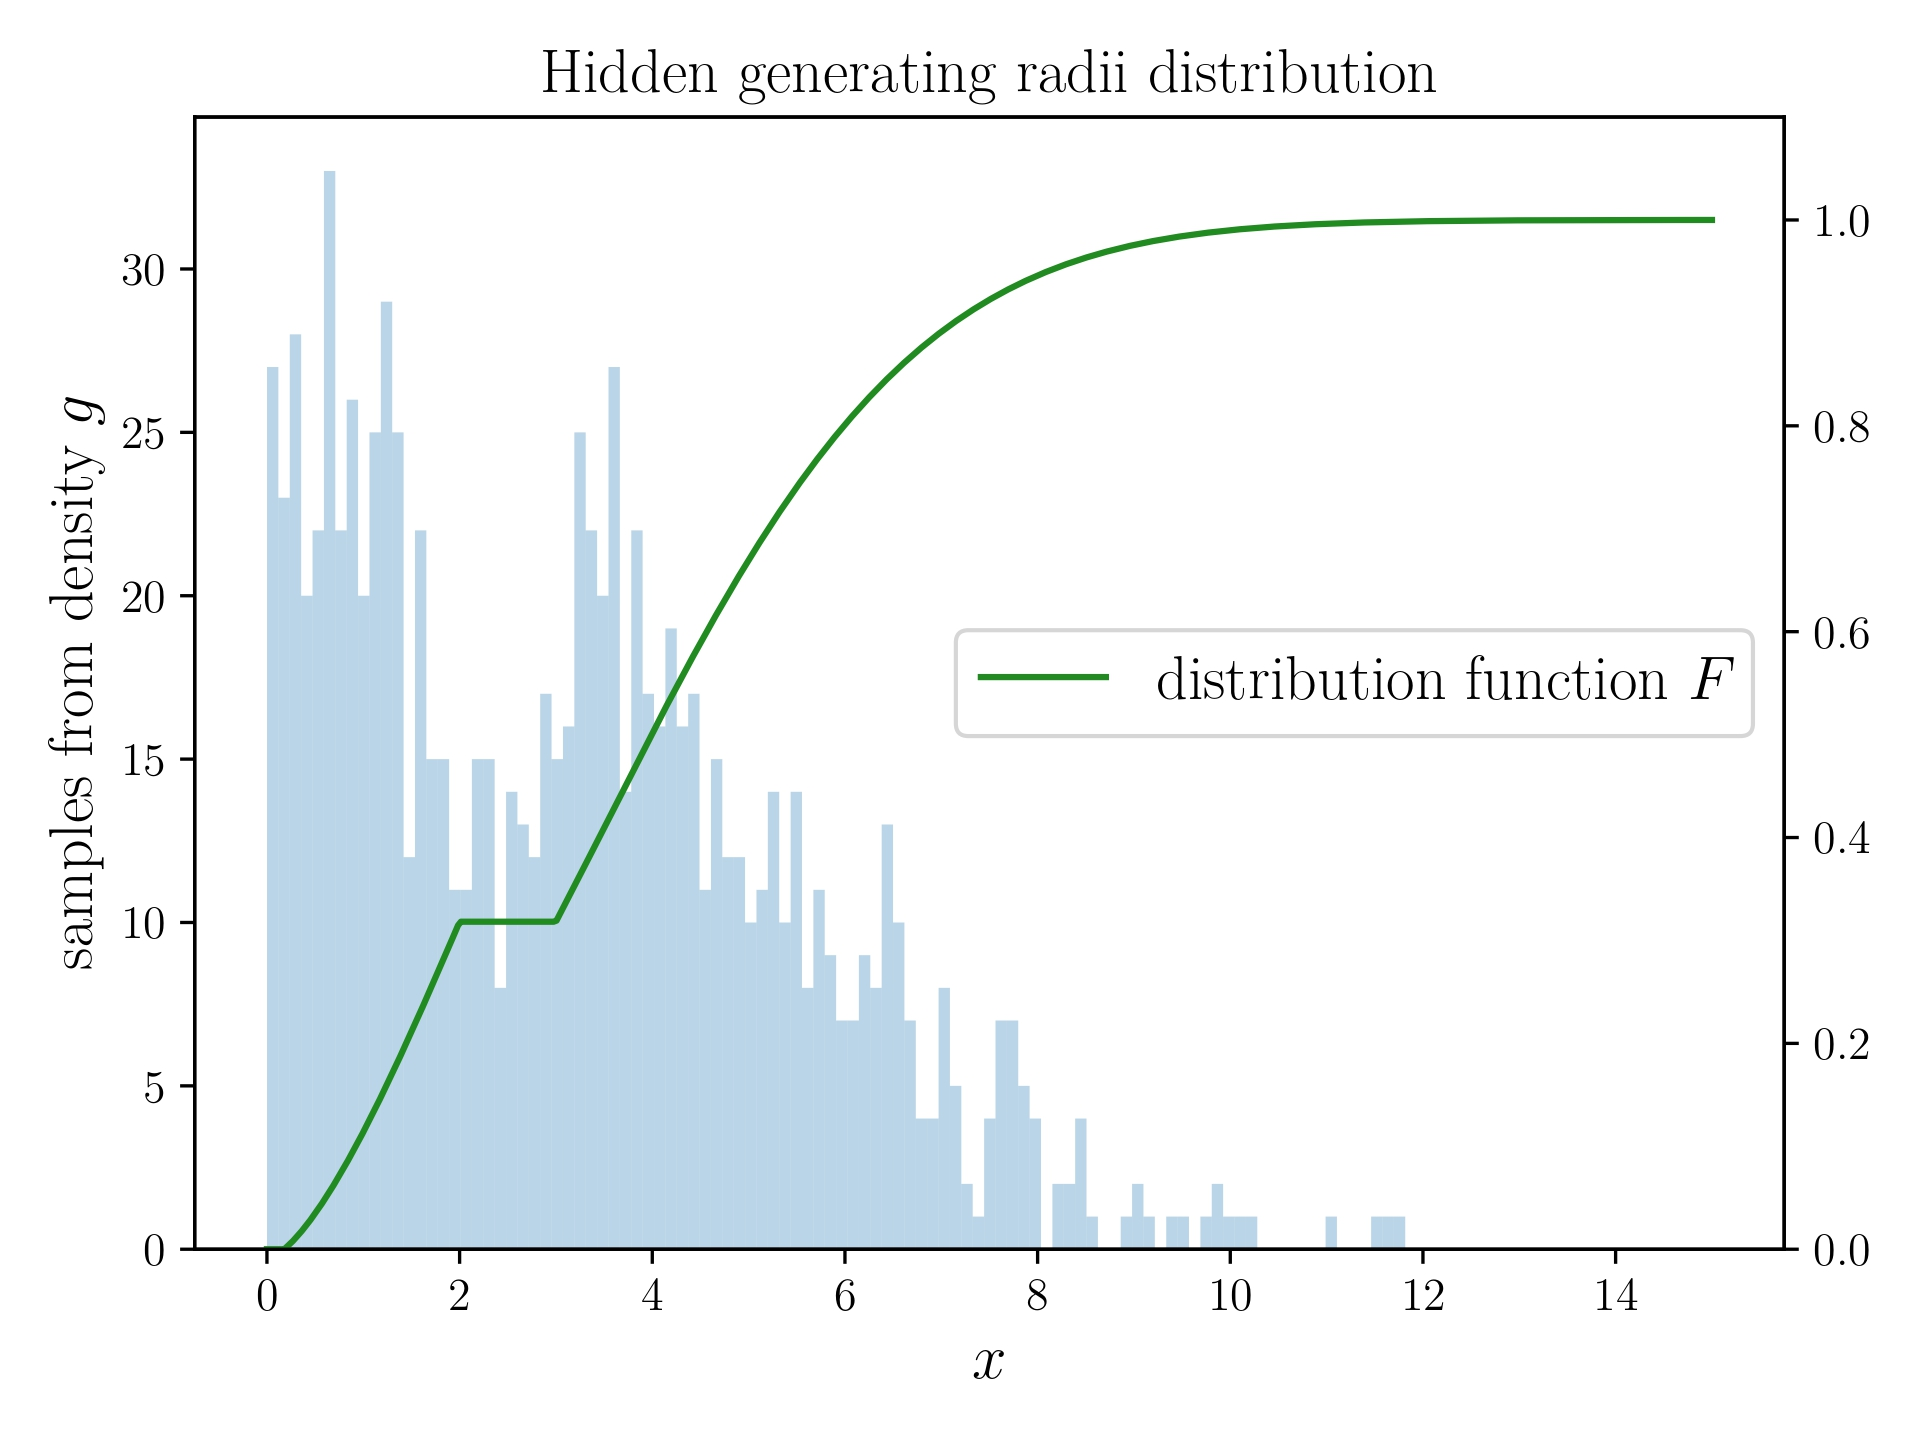
\includegraphics[width=6cm]{img/cdf_truth_page.jpg}
  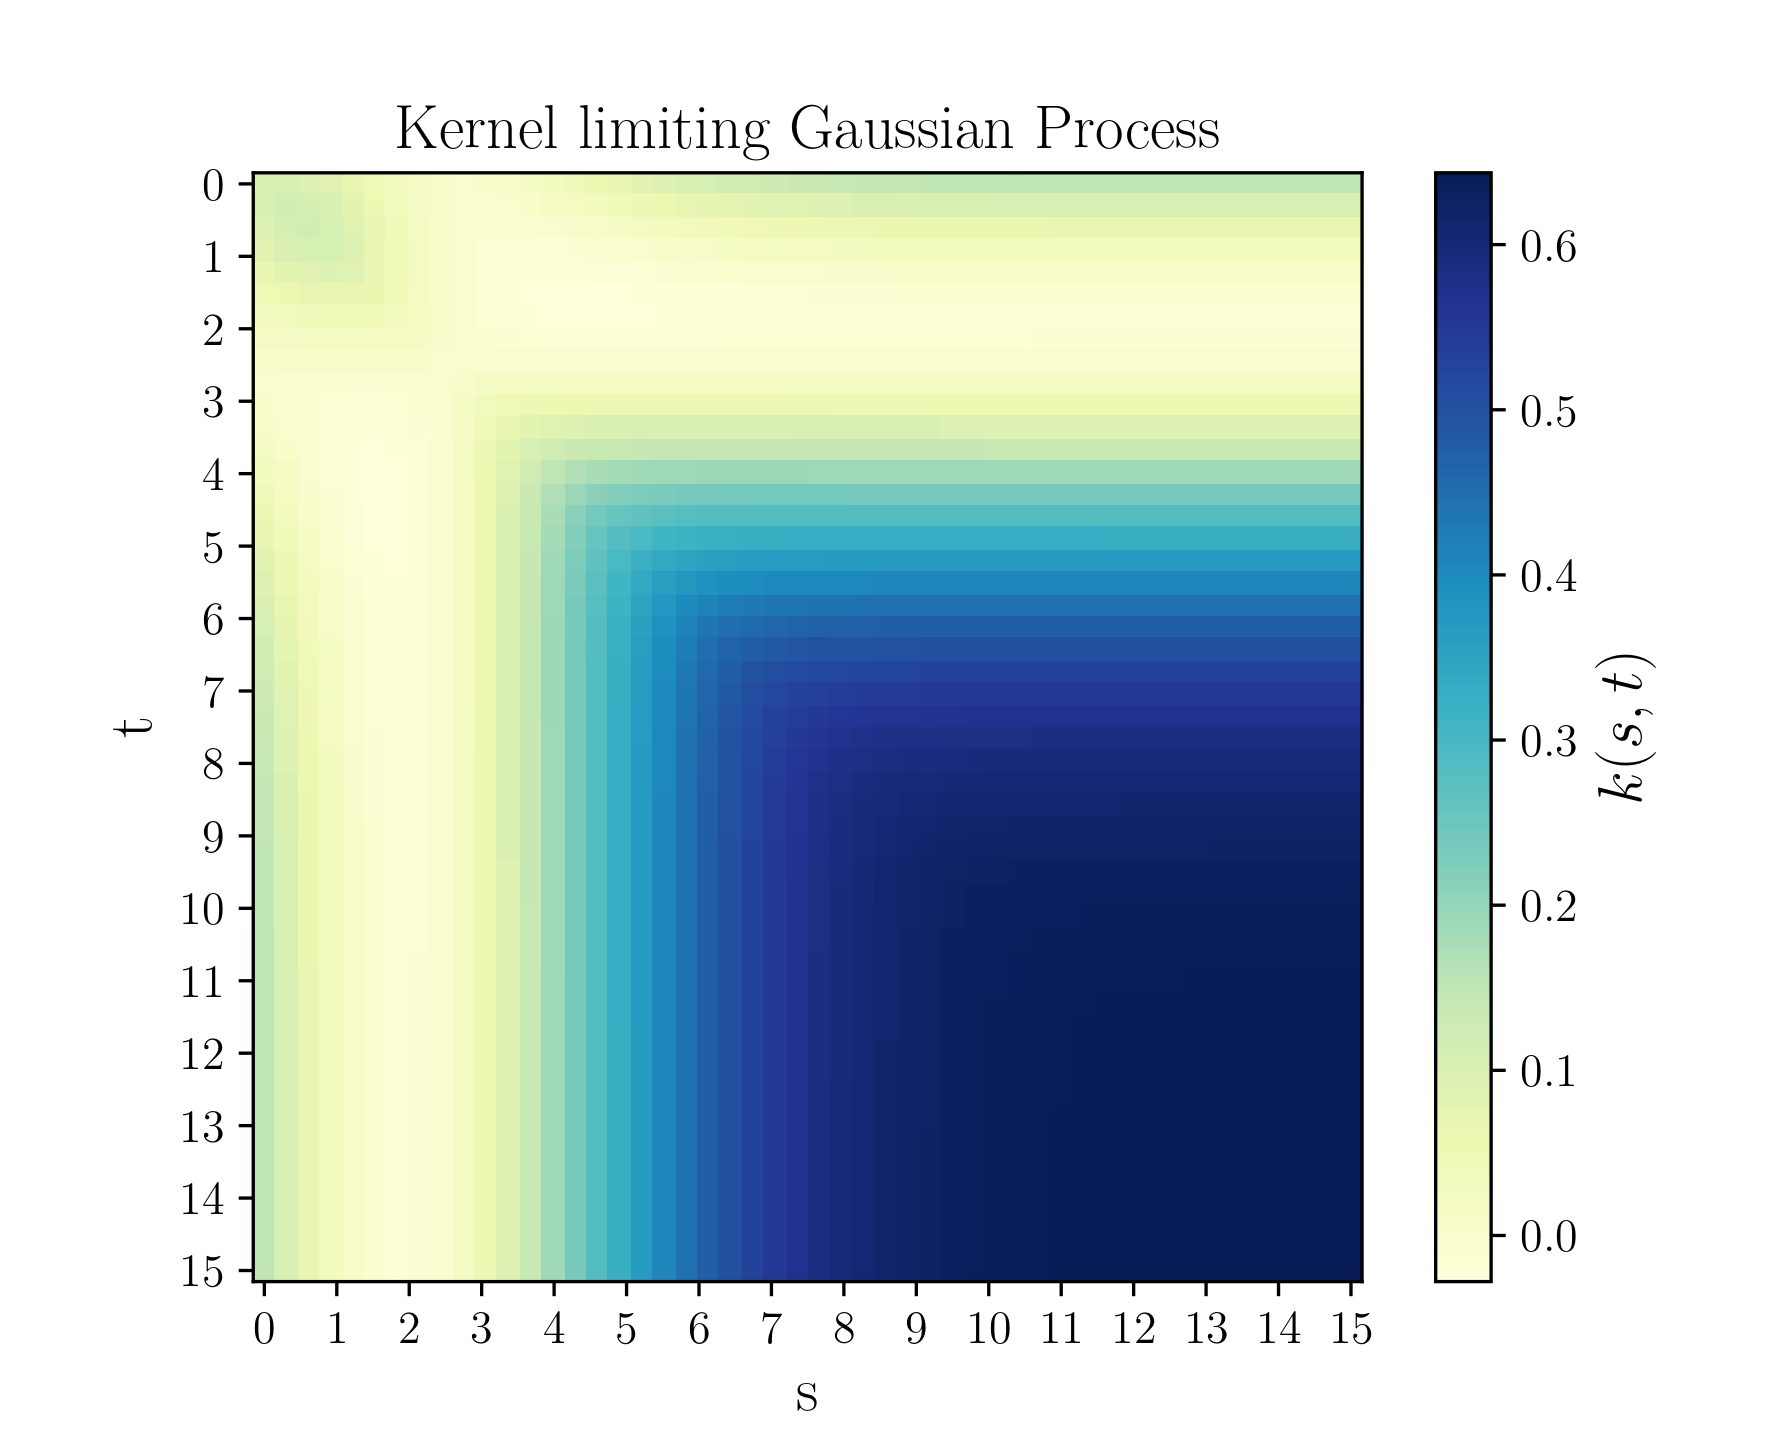
\includegraphics[width=5.75cm]{img/kernel_page.jpg}
  \setlength{\belowcaptionskip}{-4pt}
  \setlength{\abovecaptionskip}{0pt}
  \caption{Left panel: underlying cdf $F^*$ with samples from $g$. Right panel: representation of covariance structure of the limiting Gaussian Process $\mathbb{Z}_x$.}\label{fig: 1}
\end{figure}
\begin{figure}[ht]
  \centering
  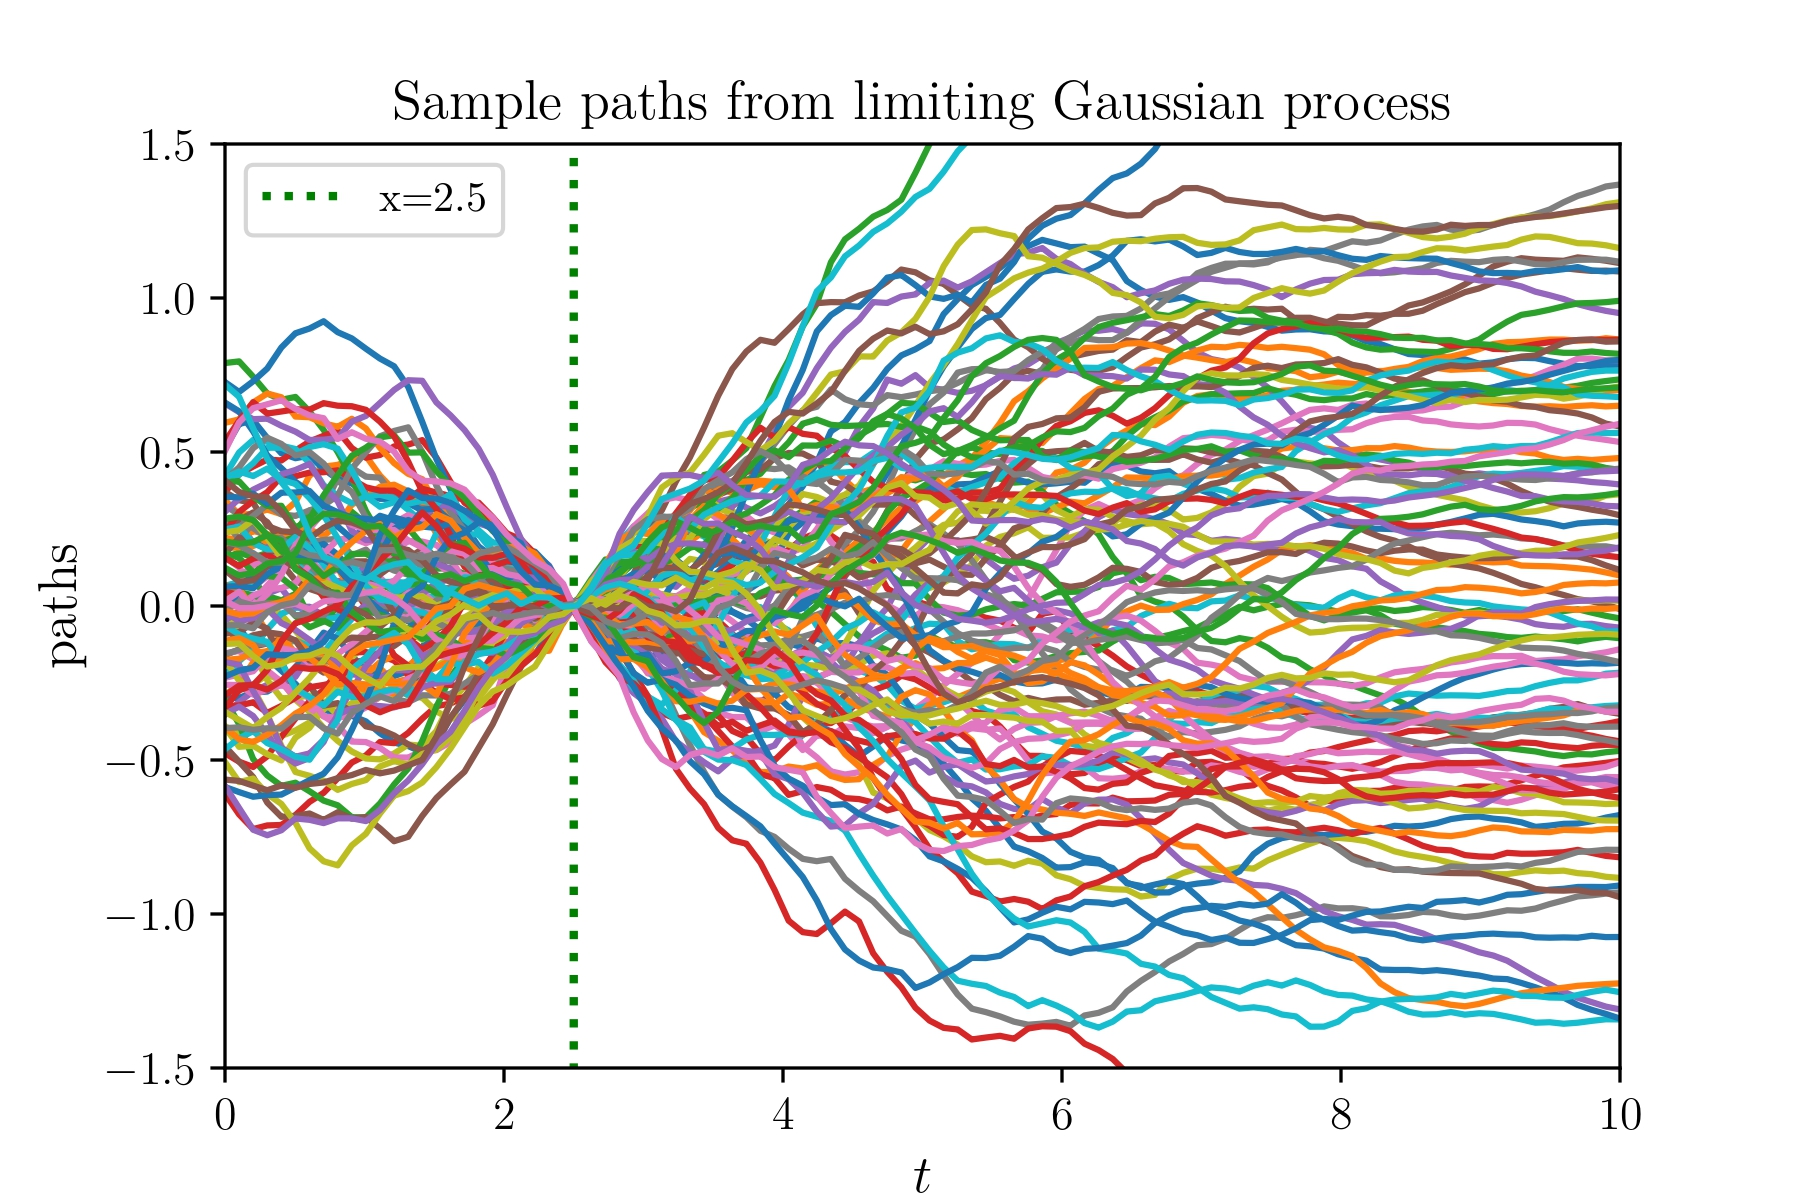
\includegraphics[width=6.2cm]{img/samplepahts_page.jpg}\hspace{-0.5cm}
  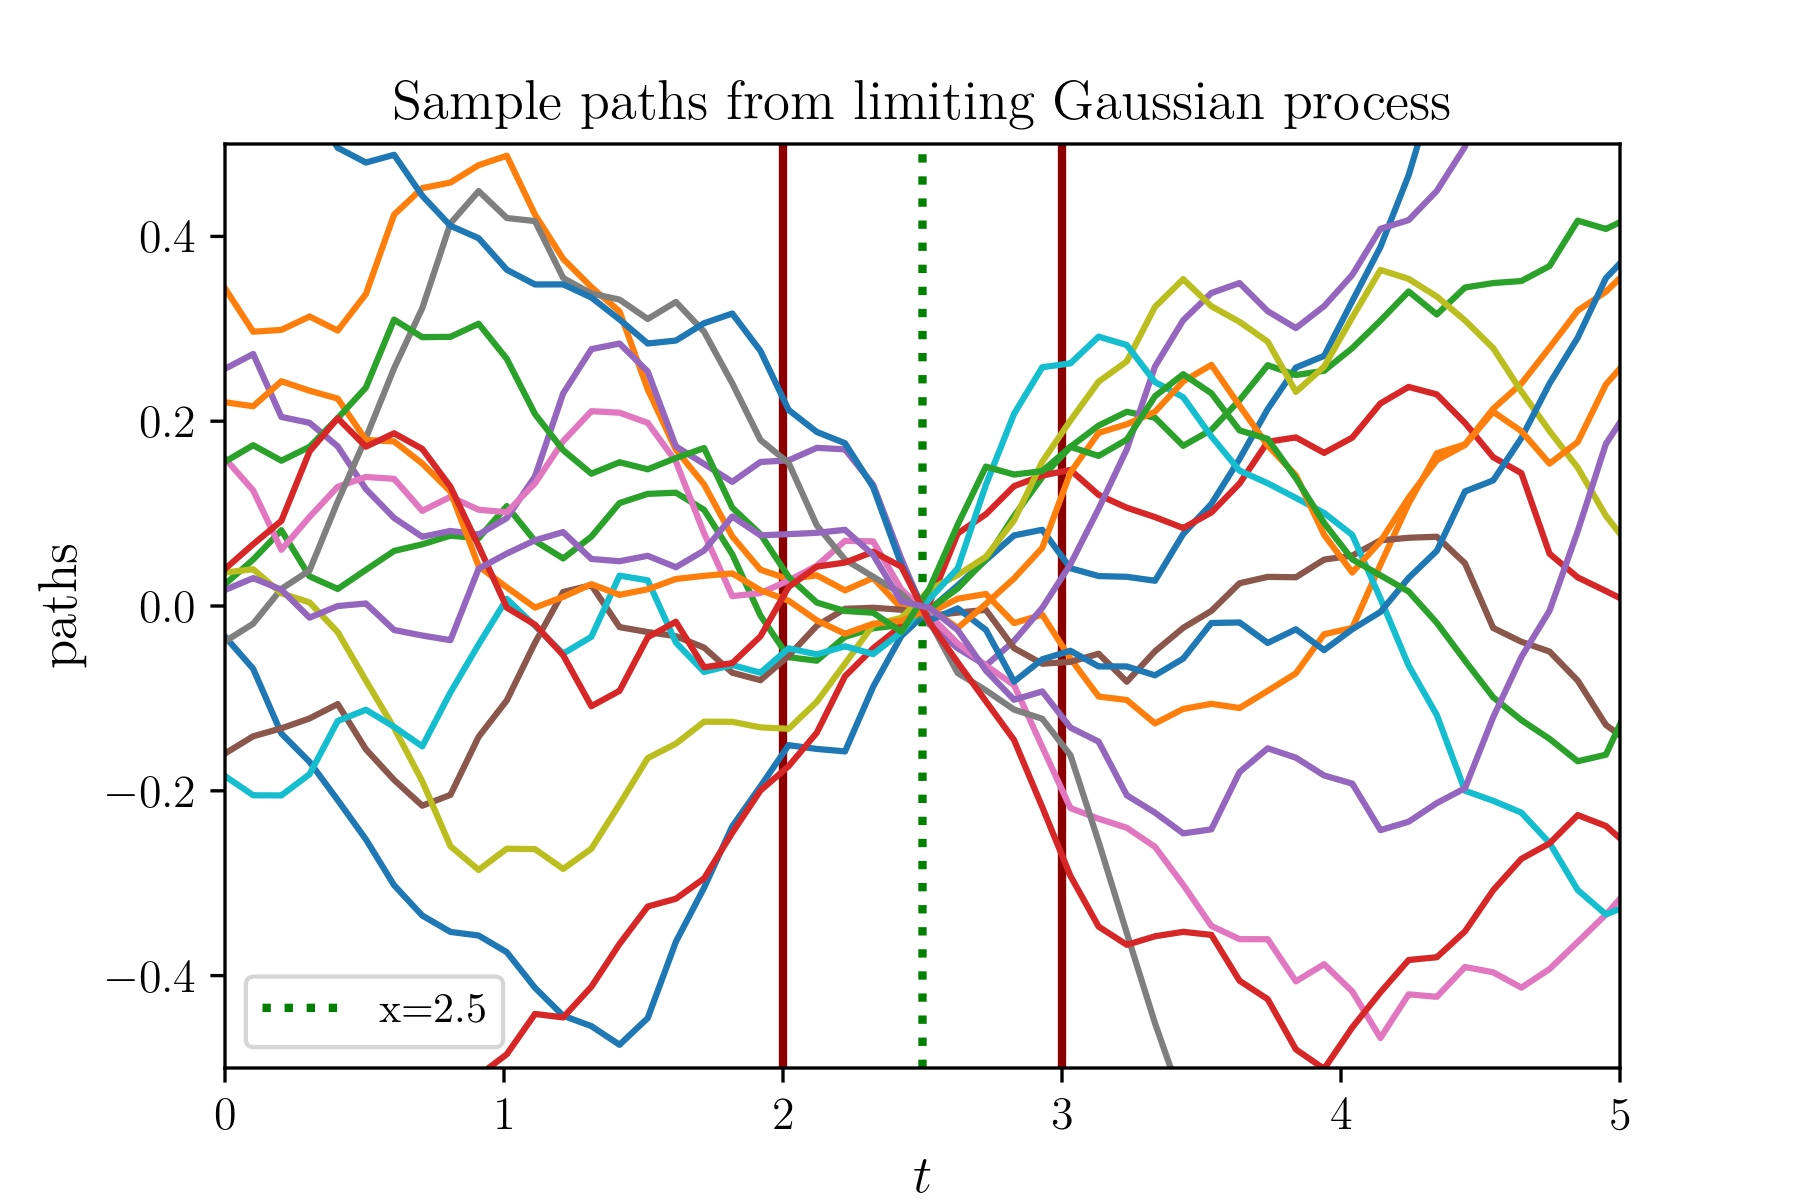
\includegraphics[width=6.2cm]{img/zoomsamplepahts_page.jpg}
  \setlength{\belowcaptionskip}{-4pt}
  \setlength{\abovecaptionskip}{-4pt}
  \caption{Left panel: $200$ samples from limiting Gaussian Process $\mathbb{Z}_x$. Right panel: zoom in on $15$ samples paths, putting into evidence the interval $[2,3]$.}\label{fig: 2}
\end{figure} 


In this setting, we show some simulations of the distribution of the limiting random variable of Theorem \ref{thm: distrib flat F at x}, above denoted by $L_x$. To do that, we compute the kernel given in \eqref{eq: covariance gauss process} of the limiting Gaussian process $\mathbb{Z}_x$. For the $F^*$ given in the left panel of Figure \ref{fig: 1}, the corresponding kernel is given in the right panel of Figure \ref{fig: 1}.
Subsequently, we simulate $200$ sample paths from the limiting Gaussian Process $\mathbb{Z}_x$ with the given kernel. These sample paths are shown in Figure \ref{fig: 2}. In the right panel of Figure \ref{fig: 2} we zoom in on the interval $[2,3]$ of interest and look at the behavior of $15$ selected sample paths. As we would expect, all sample paths pass through $(2.5,0)$.

In order to simulate the distribution of $L_x$, we use the fact that such random variable, by the proof of the theorem, is the right derivative of the least concave majorant of the Gaussian Process $\mathbb{Z}_x$ evaluated at $x = 2.5$.  With all the gathered samples from $L_x$ we looked at its estimated distribution and below we show some tests about the normality of the distribution of $L_x$. With the gathered samples, we see in Figure \ref{fig: 3} that we could not reject the null hypothesis that $L_x$ is normally distributed.

\begin{figure}
   \vspace{-0.1cm} 
  \centering
  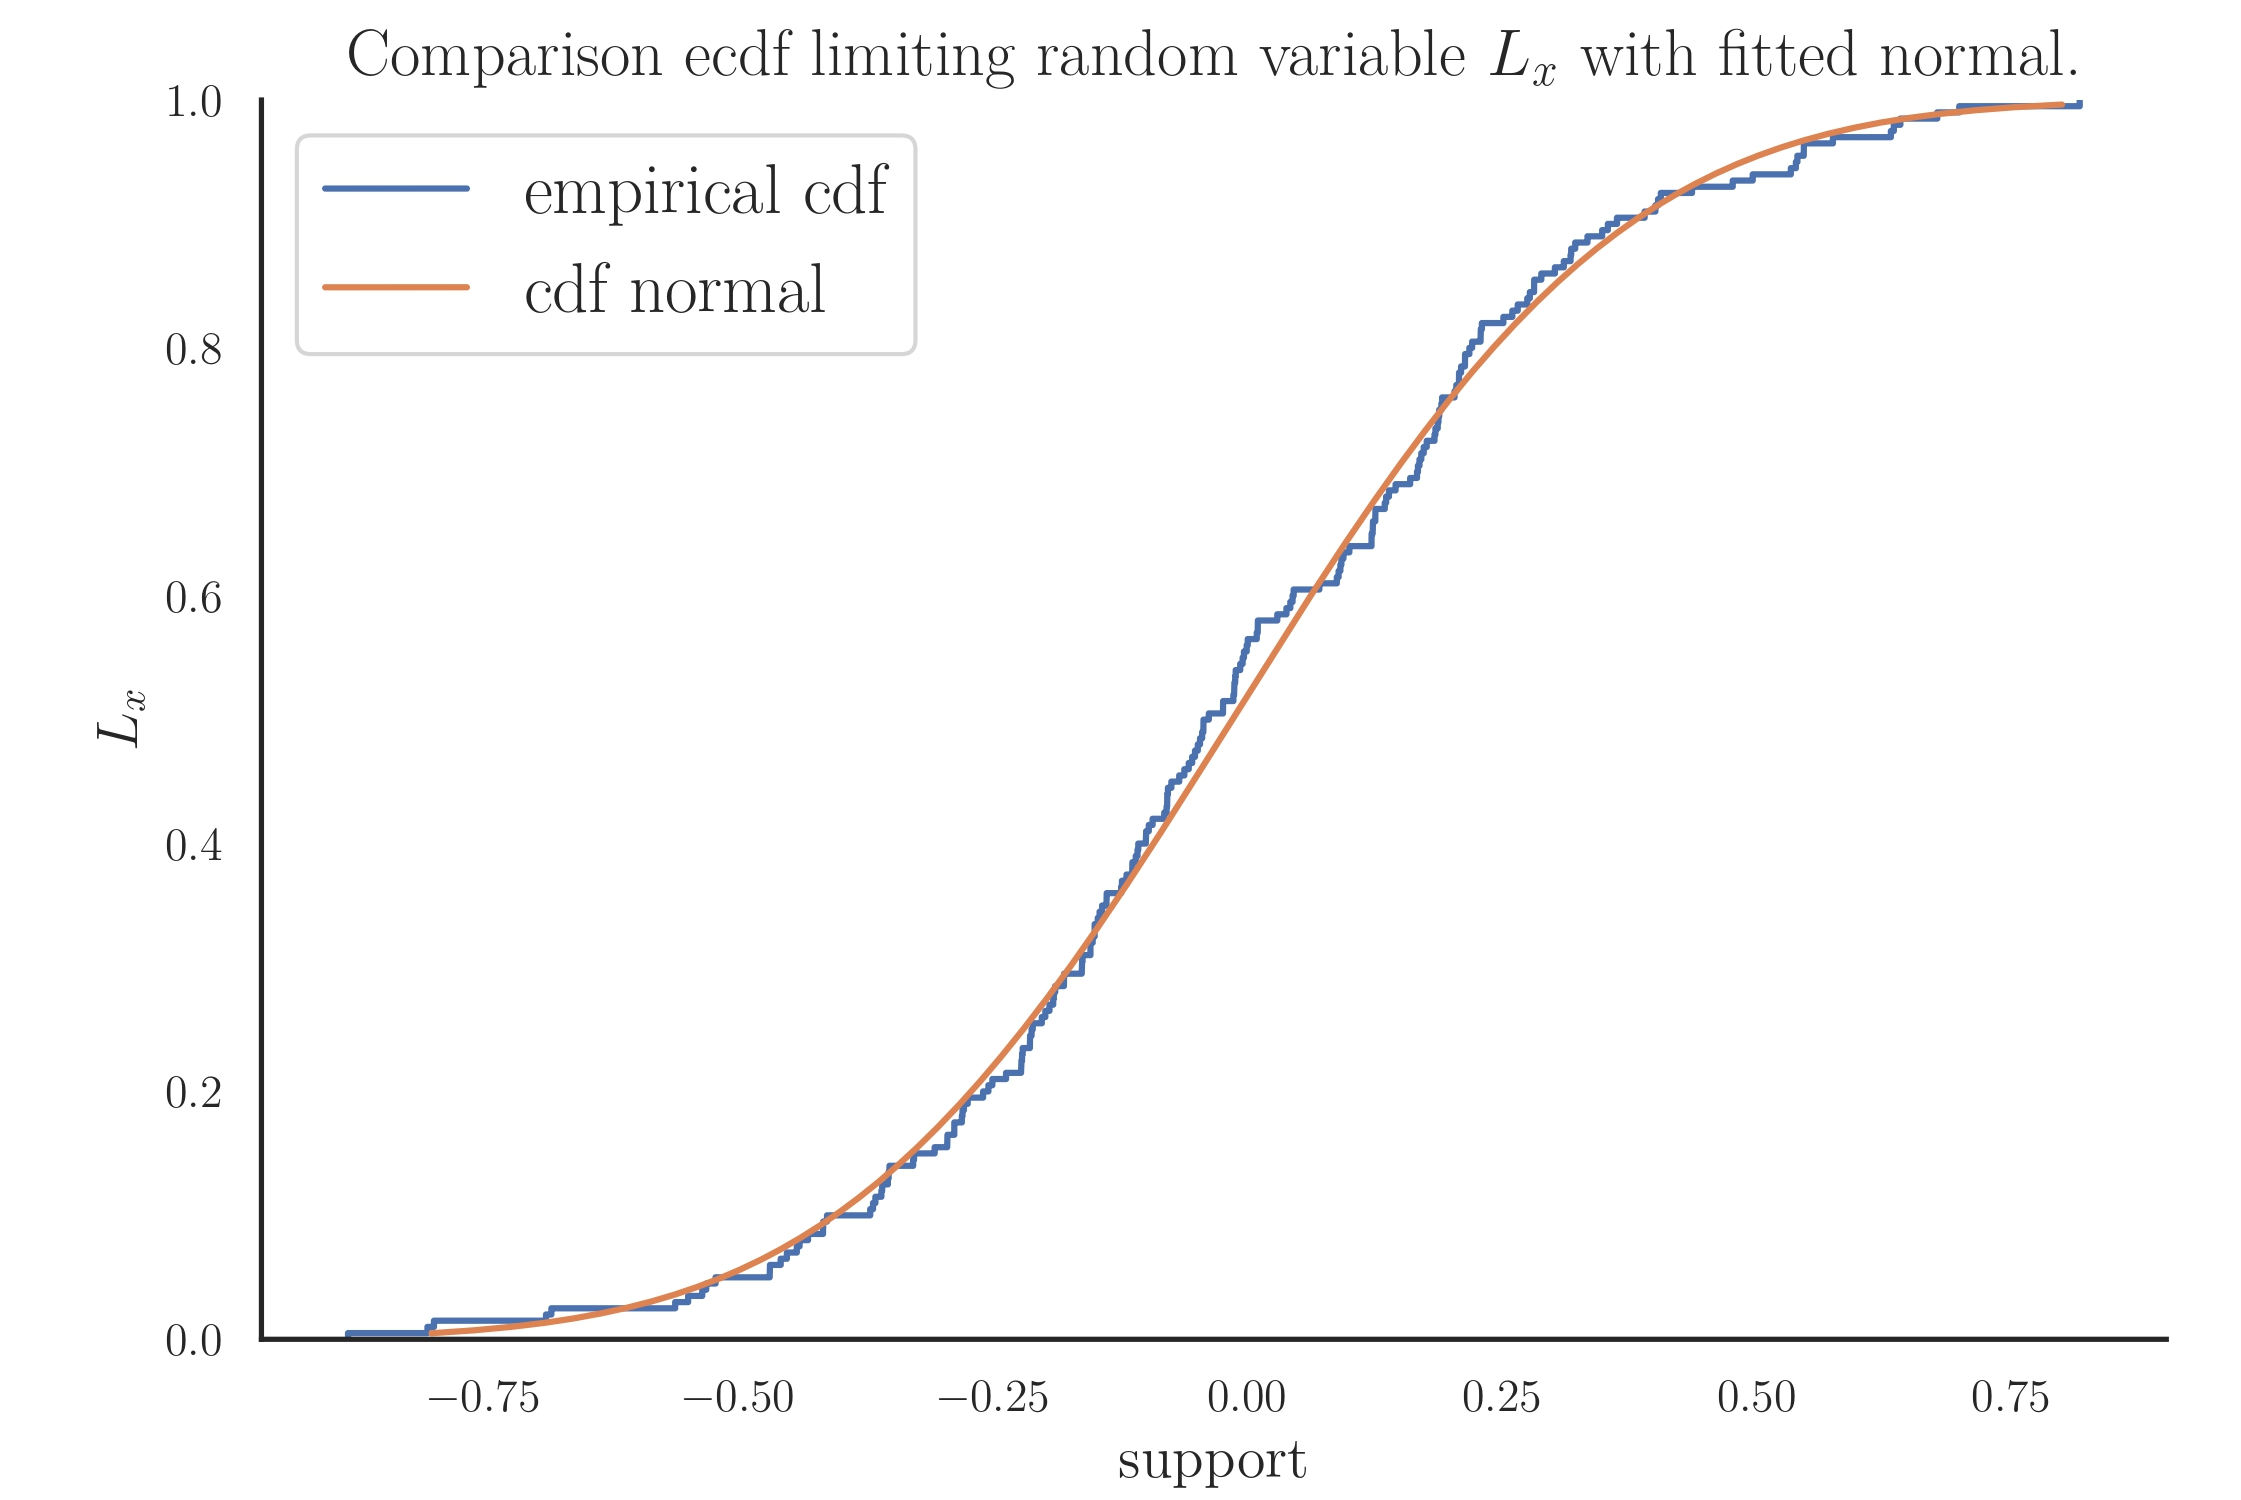
\includegraphics[width=6cm]{img/ecdfvsnormal_page.jpg}\hspace{-0.3cm}
  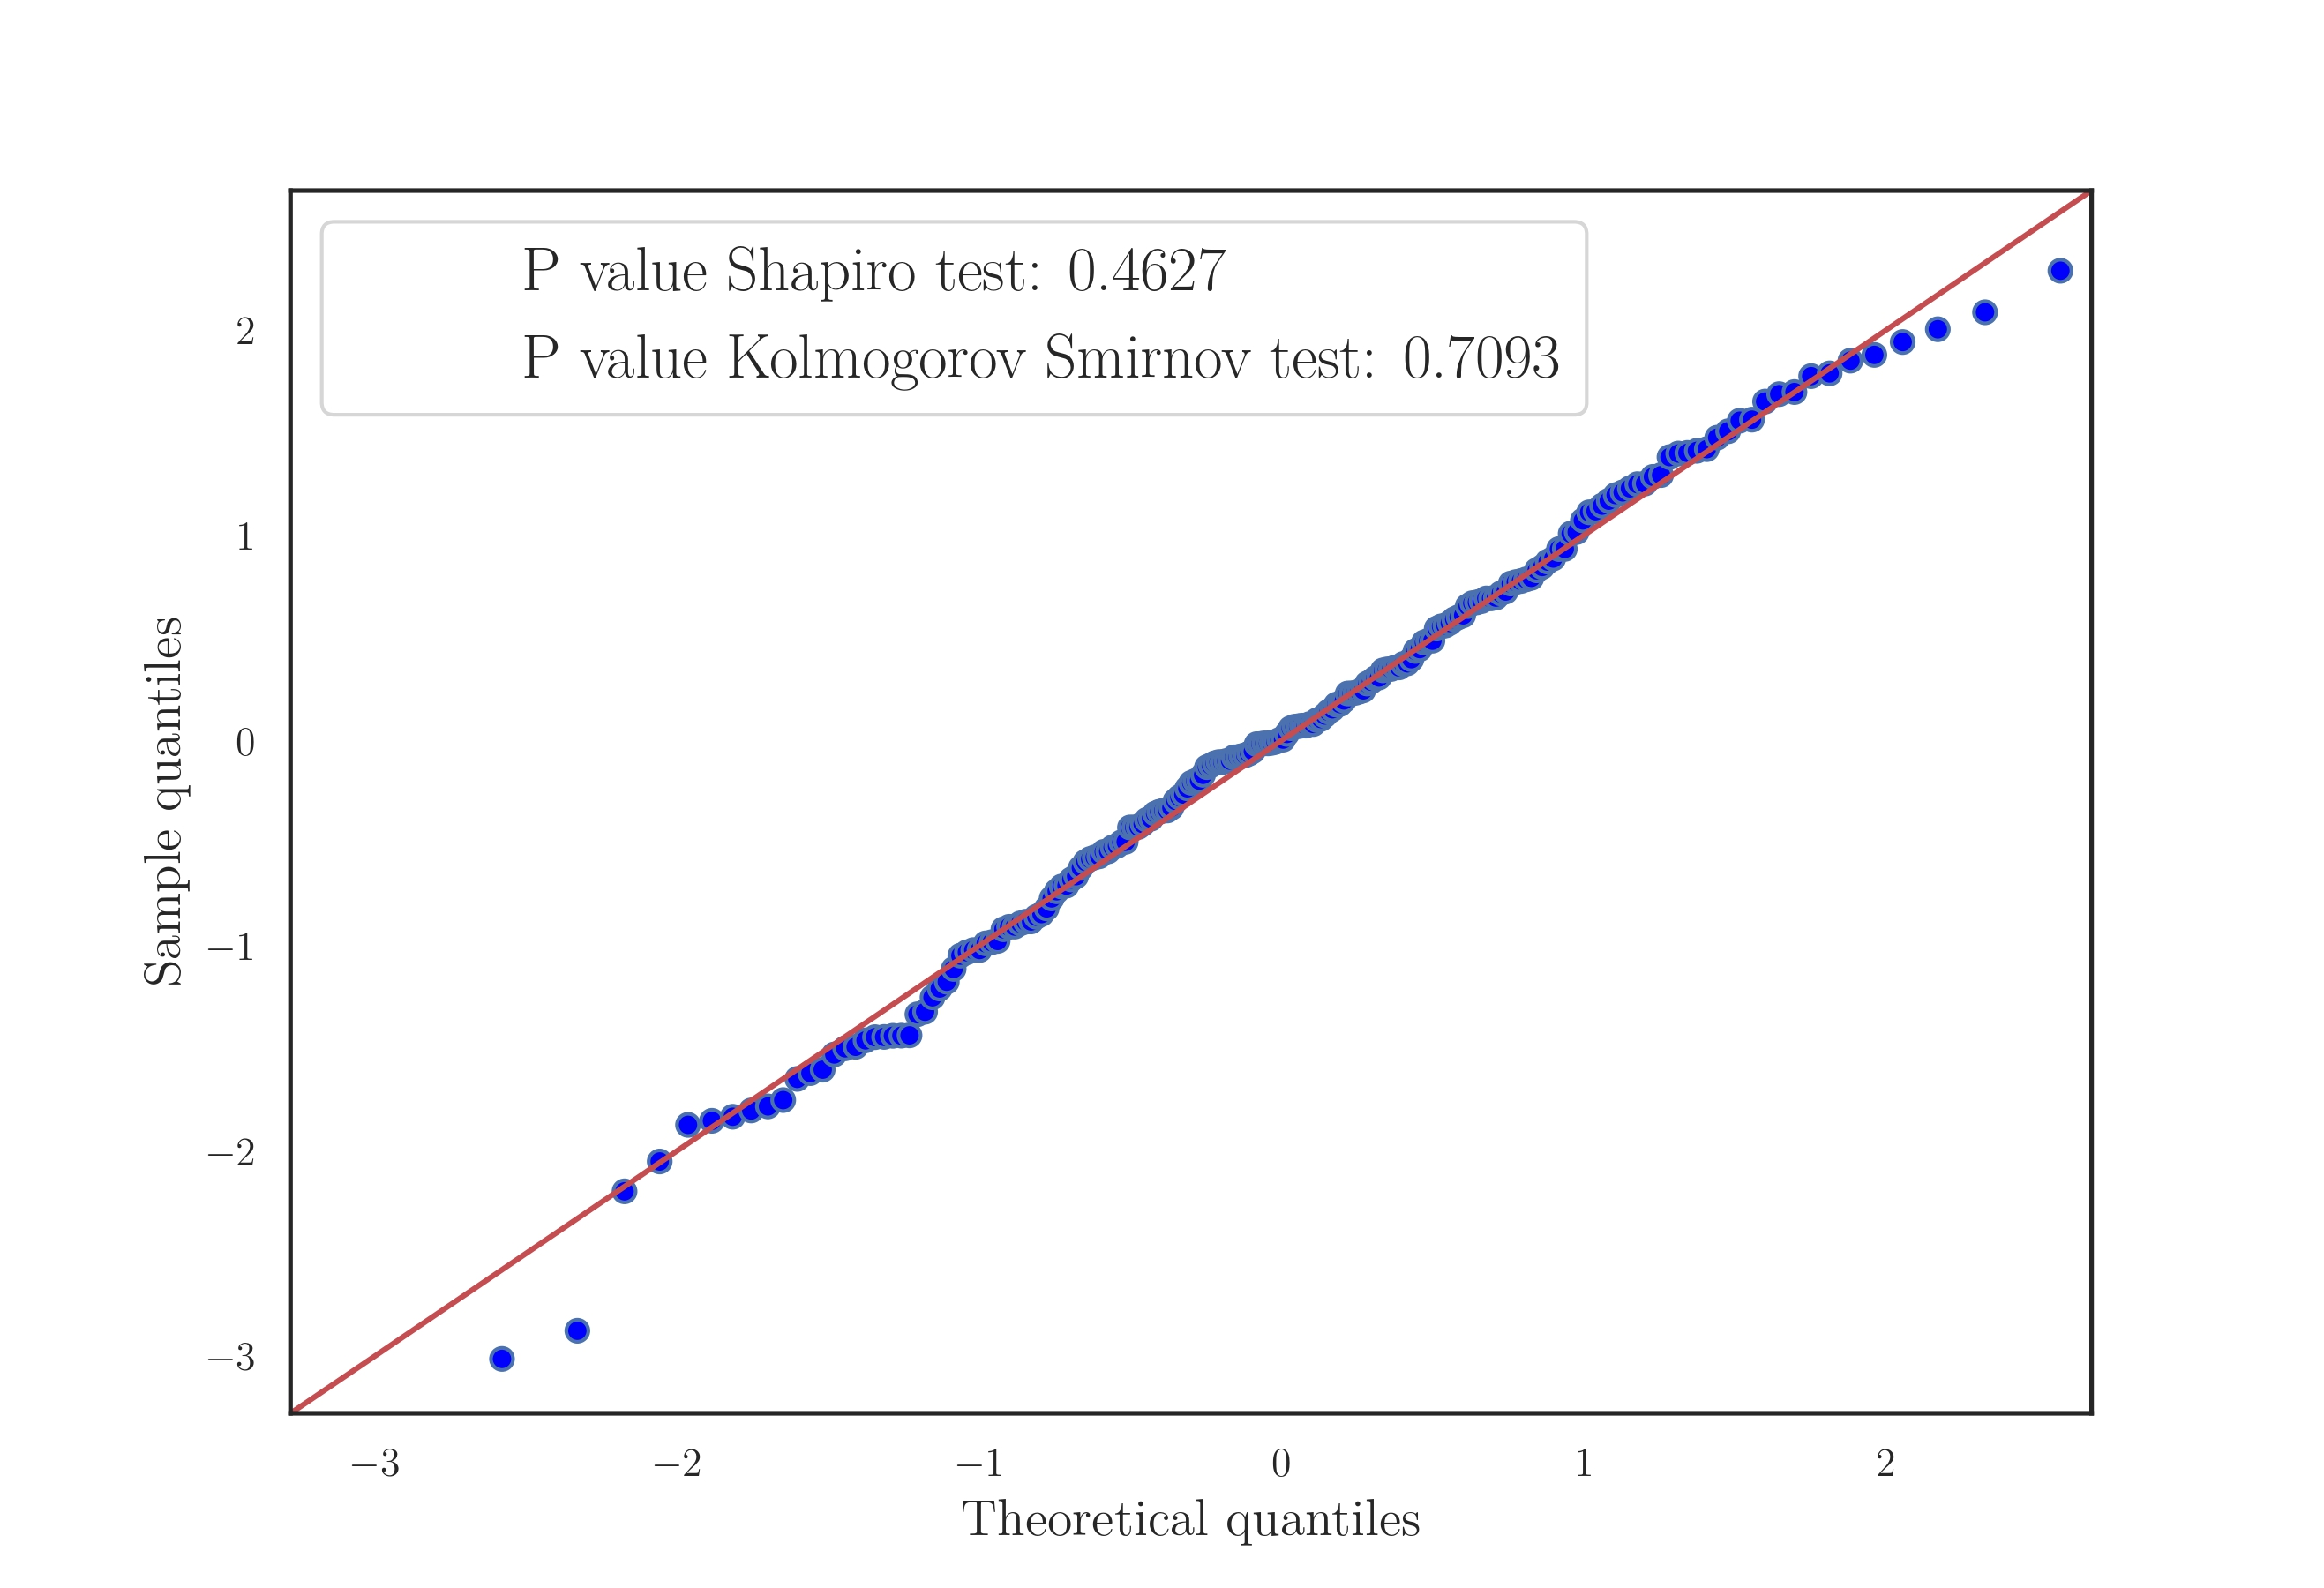
\includegraphics[width=6.5cm]{img/pvalues_page.jpg}
  \setlength{\belowcaptionskip}{-6pt}
  \setlength{\abovecaptionskip}{-4pt}
  \caption{Left panel: ecdf of limiting random variable $L_x$ compared to a suitably fitted normal. Right panel: qq-plot of $L_x$ compared to the fitted normal and p-values of the standard tests.}\label{fig: 3}
\end{figure}



\subsection{Local Asymptotic Minimax Theorem}

In this subsection, we show that the isotonic estimator (IIE) is asymptotically efficient, in the sense that its asymptotic variance is the smallest attainable. For this reason, we establish a statement about a lower bound of the minimax risk for any estimator sequence. We do this by constructing a parametric perturbation along the least favorable direction in the proximity of the true distribution function $F^*$. 

Let $x > 0$ be the point at which we want to estimate $F^*$. The existence of a least favorable path is a non-trivial matter. We will be guided by intuition in the construction of this path. We want to estimate is: $F^*(x) = 1 - V(x)/V(0)$. The local behavior at $x$ and $0$ of the kernels in the definitions of $V(x)$ and $V(0)$ is what essentially characterizes the estimation in Wicksell's problem and leads to the unusual rate $n^{-1/2}\sqrt{\log{n}}$. Thus, it should be enough to introduce a local perturbation of $F^*$ around $x$ and $0$. However, such perturbation must be tailored according to the local level of smoothness of the true $F^*$ near $x$ and $0$. Therefore, we need to identify such a level, and this is done in the following condition \eqref{eq: condition roughness infimum}.

The level of locality of the condition must be tied to the smoothness itself, because if the true $F^*$ is very rough around $x$ or $0$, then we expect a more stringent level of locality (and vice versa). Therefore we define the following intervals close to $p \in \{0,x\}$ for constants $\gamma_0 > \frac{1}{2}, \gamma_x > \frac{1}{2}$ to be determined later:
\begin{gather*}
\prescript{r}{}{\mathrm{K}}^{0}_n := \left[ n^{-\frac{1}{2\gamma_{\scaleto{0}{2.5pt}}}}, \eta_n  \right],\\
\prescript{l}{}{\mathrm{K}}^{x}_n := \left[ x - \eta_n, x - n^{-\frac{1}{2\gamma_{\scaleto{x}{2.5pt}}}} \right], \: \: \: \prescript{r}{}{\mathrm{K}}^{x}_n := \left[ x + n^{-\frac{1}{2\gamma_{\scaleto{x}{2.2pt}}}},x + \eta_n  \right],
\end{gather*}
where $\eta_n \downarrow 0$, $0 < \eta_n \leq 1, \: \forall \, n$ and $\exists \: \alpha \in (0,1)$ such that $\eta_n \gtrsim \frac{1}{\log^{\alpha}(n)}$. Now, let $\gamma_0, \gamma_x$ be the smallest constants greater than $1/2$, such that the true $F^*$, for $\mathrm{K}^p_n \in \{ \prescript{r}{}{\mathrm{K}}^{x}_n, \prescript{l}{}{\mathrm{K}}^{x}_n, \prescript{r}{}{\mathrm{K}}^{0}_n\}$ and therefore $p \in \{0,x\}$ satisfies:
\begin{align*}
    &\liminf_{n \rightarrow \infty } \inf_{\substack{x_1, x_2 \in \mathrm{K}^p_n }}\sqrt{n\log{n}}  \frac{|F^*(x_2)-F^*(x_1)|}{\Big|\log{\left\{\frac{p-x_1}{p-x_2} \right\}}\Big|} = \infty. \numberthis \label{eq: condition roughness infimum} 
\end{align*}

With condition \eqref{eq: condition roughness infimum}, our path can be shown to be well-defined and it is the least restrictive we can require. As we naturally would expect, the $\gamma_0, \gamma_x$ introduced above contain information about the local roughness of $F^*$ near $x$ and $0$. We illustrate this with our previous example \ref{example: cdf holder} and an additional example.
\begin{example}
Let us consider the same class of functions as in Example \ref{example: cdf holder}. These functions can be thought to be tightly Hölder smooth at $x$ and satisfy \eqref{eq: condition roughness infimum}. Let us consider the interval $\prescript{r}{}{\mathrm{K}}^{x}_n =\left[x+n^{-1 /(2 \gamma_x)}, x+\log (n)^{-\alpha}\right]$. If $F^*(u)=F^*(x)+K(u-x)^{\gamma_x}$ for $u \in \prescript{r}{}{\mathrm{K}}^{x}_n$, then
$$
\begin{aligned}
&\inf _{x_1, x_2 \in \prescript{r}{}{\mathrm{K}}^{x}_n}  \frac{\left|F^*\left(x_2\right)-F^*\left(x_1\right)\right|}{\left|\log \left\{\left(x-x_1\right) /\left(x-x_2\right)\right\}\right|} =K \inf_{ \substack{x_1, x_2 \in \prescript{r}{}{\mathrm{K}}^{x}_n \\ x_1<x_2}} \frac{\left(x_2-x\right)^{\gamma_x}-\left(x_1-x\right)^{\gamma_x}}{\log \left\{1+\left(x_2-x_1\right) /\left(x_1-x\right)\right\}}  \\
&=K \inf _{\substack{x_1, x_2 \in \prescript{r}{}{\mathrm{K}}^{x}_n \\ x_1<x_2}}\left(x_1-x\right)^{\gamma_x} \frac{\left[1+\left(x_2-x_1\right) /\left(x_1-x\right)\right]^{\gamma_x}-1}{\log \left[1+\left(x_2-x_1\right) /\left(x_1-x\right)\right]}  =K \gamma_x \inf _{x_1 \in \prescript{r}{}{\mathrm{K}}^{x}_n }\left(x_1-x\right)^{\gamma_x} \\
&=K \gamma_x n^{-1 / 2},
\end{aligned}
$$
because $\frac{(1+y)^\gamma-1}{\log (1+y)}$ is increasing in $y>0$ with limit $\gamma$ as $y \downarrow 0$.
\end{example}
\begin{example}
Condition \eqref{eq: condition roughness infimum}, which is similar to the conditions of \cite{10} (cf. (24) and (25)), is a consequence of a stronger on, namely: 
$$\liminf_{n \rightarrow \infty } \inf \frac{|F^*(x_2)-F^*(x_1)|}{|x_2 - x_1|^{\gamma_{\scaleto{x}{2.2pt}}} } > 0,$$ 
where the infimum is as in \eqref{eq: condition roughness infimum}. We show that it implies \eqref{eq: condition roughness infimum} on $\prescript{r}{}{\mathrm{K}}^{x}_n$:
\begin{align*}
    \inf_{\substack{x_1, x_2 \in \prescript{r}{}{\mathrm{K}}^{x}_n}} &\frac{F^*(x_2) - F^*(x_1)}{\log{\{\frac{x-x_1}{x-x_2} \}}} = \inf_{\substack{x_1, x_2 \in \prescript{r}{}{\mathrm{K}}^{x}_n }} \frac{|F^*(x_2)-F^*(x_1)|}{|x_2 - x_1|^{\gamma_{\scaleto{x}{2.2pt}}} } \frac{|x_2 - x_1|^{\gamma_{\scaleto{x}{2.2pt}}}}{\log{\left( 1 - \frac{x_2 - x_1}{x_2-x} \right)}}
\end{align*}
where, $x_1 < x_2$, both $x_1, x_2 \in \prescript{r}{}{\mathrm{K}}^{x}_n$ and thus $0<\frac{x_2 - x_1}{x_2 - x} <1$ going to zero as $n \rightarrow \infty$. The above expression, for all $n$ big enough behaves like in the previous example. Multiplied by $\sqrt{n\log{n}}$ \eqref{eq: condition roughness infimum} diverges to $\infty$.
\end{example}

The second fundamental assumption to obtain our minimax lower bound is that $g$ is continuous in a neighborhood of $x$ and in a right neighborhood of $0$. We will assume this all along. A sufficient condition to obtain this is that $F^*$ is locally Hölder continuous around $x$ and $0$ of degrees greater than $\frac{1}{2}$ (see Lemma \ref{lemma: bounded density} in Appendix \ref{sec: appendix chapter2}). We also note that from \eqref{eq: condition roughness infimum} we have $F^*(x)<1$.

We will now proceed with the construction of the path on the space of distribution functions and verify that it is well defined. The construction of our path is based on ideas from \cite{10}. Condition \eqref{eq: condition roughness infimum} gives us the appropriate $\gamma_0, \gamma_x$ that we use for the definition of the perturbation.
 For $u \geq 0$ define: 
\begin{align}\label{eq: path}
    F^*_{h_n}(u) = \frac{1}{D_{h_n}} \left( F^*(u) + h_{1,n} \int_{0}^{u} \chi_{{\scaleto{1,n}{4.5pt}}}(v) \, dv + h_{2,n} \int_{0}^{u} \chi_{{\scaleto{2,n}{4.5pt}}}(v-x) \, dv \right),
\end{align}
where for $\gamma_0 > \frac{1}{2}, \: \gamma_x > \frac{1}{2}$, using that $\int_{0}^{\infty} \chi_{{\scaleto{2,n}{4.5pt}}}(v-x) \, dv = 0$:
\begin{align*}
    &\chi_{{\scaleto{1,n}{4.5pt}}}(v)= (v)^{-1} \ind_{\left\{ n^{-1/(2\gamma_{\scaleto{0}{2.2pt}})} \leq v \leq \eta_n \right\}},  \\
    &\chi_{{\scaleto{2,n}{4.5pt}}}(v-x)= (v-x)^{-1} \ind_{\left\{ n^{-1/(2\gamma_{\scaleto{x}{2.2pt}})} \leq|v-x| \leq \eta_n \right\}}, \\
    &D_{h_n} = 1 + h_{1,n} \int_{0}^{\infty} \chi_{{\scaleto{1,n}{4.5pt}}}(v) \, dv + h_{2,n} \int_{0}^{\infty} \chi_{{\scaleto{2,n}{4.5pt}}}(v-x) \, dv \\
    &\quad \quad = 1 + h_{1,n} \int_{0}^{\infty} \chi_{{\scaleto{1,n}{4.5pt}}}(v) \, dv. 
\end{align*}
We will see that the truncation levels of the function $1/(v-x)$ proposed here above work, but they may not be unique. The function $\chi_{{\scaleto{i,n}{4.5pt}}}$, with similar truncation levels, was introduced for the first time in \cite{10}, however there it was not used directly for the perturbation as done here and the assumption $\gamma_0 = \gamma_x$ was used.

We will check that the perturbation $ F^*_{h_n}$ is well defined for: 
\begin{align}\label{eq: h_i}
    h_{i,n}= \frac{h_i}{\sqrt{n \log{n}}}, \quad h_i \in \mathbb{R}, \quad i=1,2. 
\end{align}

\begin{figure}
    \vspace{-0.1cm}
  \centering
  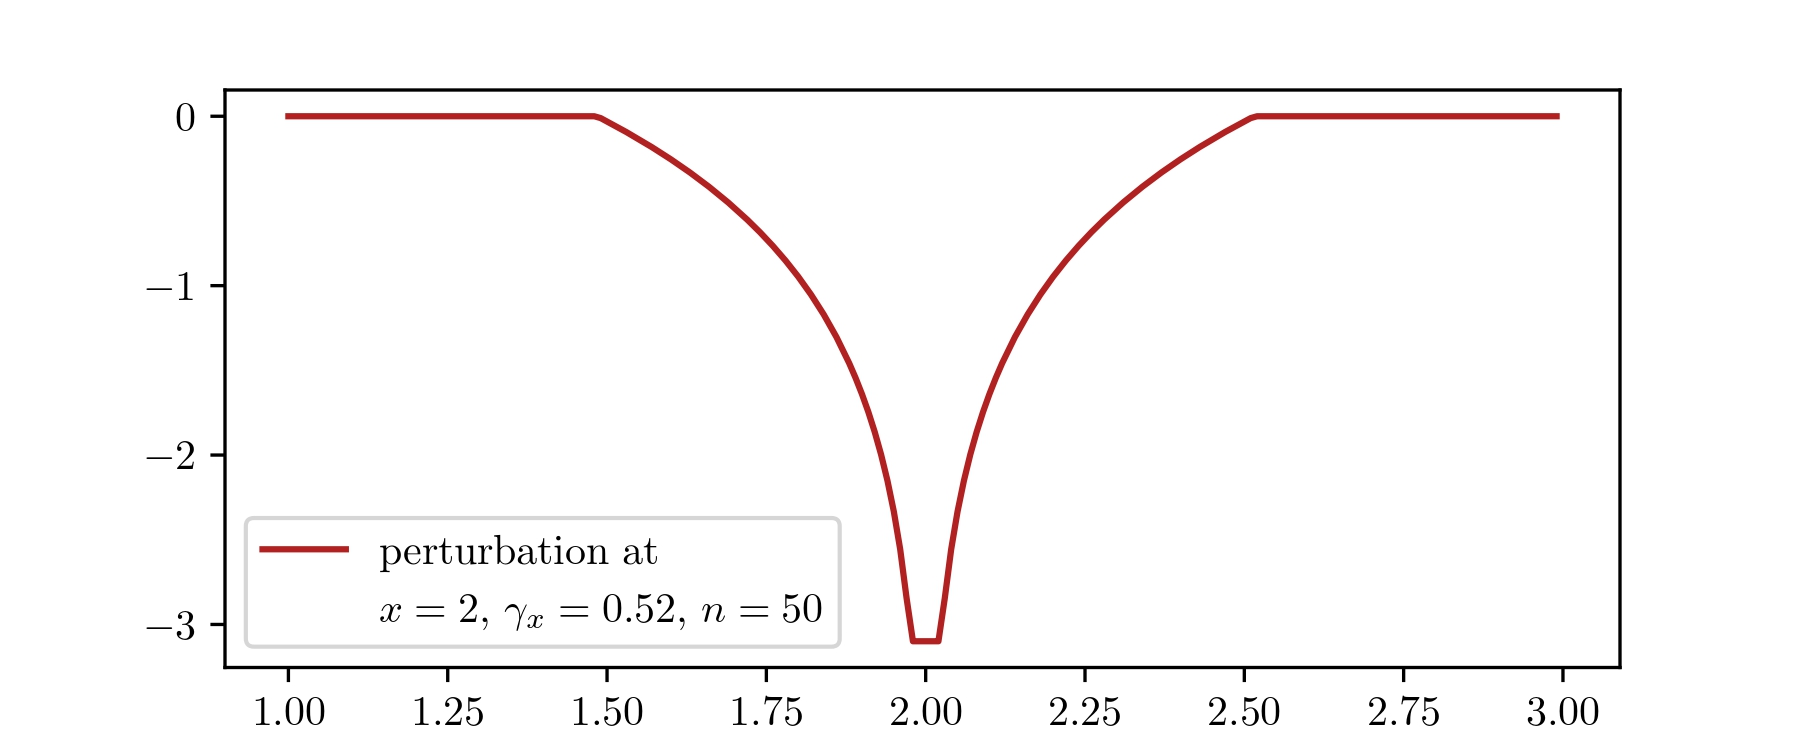
\includegraphics[width = 8cm]{img/perturbation_page.jpg}
  \setlength{\belowcaptionskip}{-4pt}
  \caption{Visualization of $\int_{0}^{u} \chi_{{\scaleto{2,n}{4.5pt}}}(v-x)dv$ for $x=2$, $n=50$ and $\gamma_x = 0.52$, $\eta_n = 1/\sqrt{\log{n}}$.} \label{fig: perturbation}
\end{figure}

First, we compute the case of $\chi_{{\scaleto{2,n}{4.5pt}}}$, to show how the perturbation looks like:
\begin{align*}
    &\int_{0}^{u} \chi_{{\scaleto{2,n}{4.5pt}}} (v-x) \, dv = \log{\left(\eta^{-1}_n (x-u) \right)}\ind_{\big\{ x - \eta_n \leq u \leq x - n^{-\frac{1}{2 \gamma_{\scaleto{x}{2.2pt}}}} \big\}} +\\
    &\quad + \log{\left( \eta^{-1}_n \, n^{-\frac{1}{2 \gamma_{\scaleto{x}{2.2pt}}}} \right)} \bigg( \ind_{\big\{ u > x - n^{-\frac{1}{2 \gamma_{\scaleto{x}{2.2pt}}}} \big\}} - \ind_{\big\{ u > x + \eta_n \big\}} \bigg)+\\
    &\quad + \log{\left(\eta^{-1}_n(u-x) \right)} \ind_{\big\{x + n^{-\frac{1}{2 \gamma_{\scaleto{x}{2.2pt}}}} \leq u \leq x+\eta_n  \big\}}. \numberthis \label{eq: written out perturbation}
\end{align*}
Figure \ref{fig: perturbation} visualizes the perturbation $\int_{0}^{u} \chi_{{\scaleto{2,n}{4.5pt}}}(v-x)dv$ in \eqref{eq: written out perturbation}. It is immediate from \eqref{eq: written out perturbation} that this perturbation is continuous and therefore the summation with $F^*$ results in a function $F^*_{h_n}$ that is right-continuous. Moreover, thanks to the normalization $D_{h_n}$, $\lim_{u \rightarrow + \infty} F^*_{h_n} (u) =1$ and, from the definition of $F^*_{h_n}$, note that $\lim_{u \rightarrow 0} F^*_{h_n} (u) =0$.
What is not evident is if $F^*_{h_n}$ is non-decreasing. Intuitively, for this to be true, we need $F^*$ to be "increasing enough" to compensate for the negative drop introduced by the perturbation. Condition \eqref{eq: condition roughness infimum} ensures that this is the case.  
\begin{lemma}\label{lemma: non decreasing F_h}
    For all $n$ sufficiently large, $F^*_{h_n}$ is non decreasing.
\end{lemma}
The \hyperlink{proof of lemma 5}{proof} of this lemma is provided in Appendix \ref{sec: appendix chapter2}.  We start by stating the most interesting result of this section which is the so-called LAM (locally asymptotically minimax) theorem and it entails the minimax risk for any estimator sequence. The proof of this theorem requires a few additional technical statements (the LAN expansion and the expression of the derivative of the functional of interest), which will be provided right after.
\begin{theorem}[LAM]\label{thm: LAM}
    Let $\gamma_0, \gamma_x$ be the smallest constants above $\frac{1}{2}$ such that $F^*$ satisfies \eqref{eq: condition roughness infimum}. Let $J=  \frac{\pi^2 }{8 m^2_0 } \operatorname{diag}\left(\frac{1}{\gamma_{\scaleto{0}{2.5pt}} g(0)}, \frac{1}{ \gamma_{\scaleto{x}{2.2pt}} g(x)}\right)$, $\dot{\psi} = \begin{bmatrix} \frac{1}{2\gamma_{\scaleto{0}{2.5pt}}} (1-F^*(x)) & - \frac{1}{2\gamma_{\scaleto{x}{2.2pt}}} \end{bmatrix}^{\top}$, $g$ as in \eqref{eq: density of the observations}, and $\ell$ be a bowl-shaped loss function, i.e., $\ell$ is non-negative, symmetric and subconvex. Then for every estimator sequence $\left( F^*_n(x)\right)_{n \in \mathbb{N}}$:
    \begin{align}\label{eq: LAM}
    \sup_{\substack{I \subset \mathbb{R}^2 \\ I \: \textup{finite}}} \liminf_{n \rightarrow \infty} \sup _{h \in I} \ex_{h} \ell\left(\sqrt{\frac{n}{\log{n}}}\left(F^*_n(x)- F^*_{h_n}(x)\right)\right) \geq \ex \ell(L) .
    \end{align}
The first supremum is taken over all finite subsets $I$ of $\mathbb{R}^2$, the expectation $\ex_h$ is under $G_{F^*_{h_n}}$, the probability measures associated to the perturbed densities $g_n$ in \eqref{eq: g_n}, and $L \sim N (0, \dot{\psi}^{\top} J^{-1} \dot{\psi})$;
\begin{align*}
    {\dot{\psi}}^{\top} J^{-1} \dot{\psi} = \frac{4m^2_0}{\pi^2} \left(\frac{g(x)}{2\gamma_x} + (1-F^*(x))^2 \frac{g(0)}{2\gamma_0} \right).
\end{align*}
\end{theorem}
\begin{proof}
The proof is an immediate application of Theorem 3.11.5 from \cite{5}, using Theorem \ref{thm: LAN} and Lemma \ref{lemma: hadamard derivative} given below.
\end{proof}

Now we proceed by proving the technical results needed for the proof of Theorem \ref{thm: LAM}. First, we show that given the path \eqref{eq: path}, we can obtain a LAN expansion (see \cite{6}, Chapter 7).
In the statement of the LAN Theorem, the perturbed density of the observations $Z_i$ appears. Therefore, using \eqref{eq: path}, we derive it before proceeding:
\begin{align*}
    g_n (z) &= \frac{1}{2m_{h_n}} \int_{z}^{\infty} \frac{dF^*_{h_n} (v)}{\sqrt{v-z}}  \numberthis \label{eq: g_n} \\
    &= \frac{1}{2m_{h_n} D_{h_n}} \left\{ \int_{z}^{\infty} \frac{dF^*(v)}{\sqrt{v-z}} + h_{1,n} \int_{z}^{\infty} \frac{\chi_{{\scaleto{1,n}{4.5pt}}}(v)}{\sqrt{v-z}} \, dv + h_{2,n} \int_{z}^{\infty} \frac{\chi_{{\scaleto{2,n}{4.5pt}}}(v-x)}{\sqrt{v-z}} \, dv \right\}.
\end{align*}
where $m_{h_n} = \int_{0}^{\infty} \sqrt{s} \, dF^*_{h_n} (s)$, analogously to $m_0$.

\begin{theorem}[LAN expansion]\label{thm: LAN}
Let $\gamma_0, \gamma_x$ be constants above $\frac{1}{2}$ such that $F^*$ satisfies \eqref{eq: condition roughness infimum}. Let $g$ be continuous in a neighborhood of $x$ and in a right-neighborhood of $0$. Then for $h^{\top} = [h_1,h_2] \in \mathbb{R}^2$, $h_n = \frac{h}{\sqrt{n\log{n}}}$, $F^*_{h_n}$ as in \eqref{eq: path} and accordingly $g_n$ in \eqref{eq: g_n}:
\begin{align*}
    \sum_{i=1}^{n} \log{\frac{g_n (Z_i)}{g(Z_i)}} = h^{\top} \Delta_n - \frac{1}{2} h^{\top} J h + o_p (1),
\end{align*}
where the $o_p(1)$ is under $Z_1,\cdots,Z_n \stackrel{\scaleto{i.i.d.}{3.2pt}}{\sim} g$, for $J =  \frac{\pi^2 }{8 m^2_0 } \operatorname{diag}\left(\frac{1}{\gamma_{\scaleto{0}{2.5pt}} g(0)}, \frac{1}{ \gamma_{\scaleto{x}{2.2pt}} g(x)}\right)$ and $\Delta_n \rightsquigarrow N\left( 0, J \right)$, where:
\begin{align*}
    \Delta_n = \begin{bmatrix} \sum_{i=1}^n \frac{1}{ m_{h_n} D_{h_n} \sqrt{n\log{n}} } \left( \frac{1}{2g(Z_i)} \int_{Z_i}^{\infty} \frac{\chi_{{\scaleto{1,n}{3.5pt}}}(v)}{\sqrt{v-Z_i}} \, dv - \int_{0}^{\infty} \sqrt{v} \chi_{{\scaleto{1,n}{4.5pt}}}(v) \, dv \right)\\ \sum_{i=1}^n \frac{1}{ m_{h_n} D_{h_n} \sqrt{n\log{n}}} \left( \frac{1}{2g(Z_i)} \int_{Z_i}^{\infty} \frac{\chi_{{\scaleto{2,n}{3.5pt}}} (v-x)}{\sqrt{v-Z_i}} \, dv - \int_{0}^{\infty} \sqrt{v} \chi_{{\scaleto{2,n}{4.5pt}}}(v - x) \, dv \right) \end{bmatrix}.
\end{align*}
\end{theorem}
\begin{proof}

The structure of the proof of this result is as follows. First, we give the expansions of the functions $\int_z^{\infty} \frac{\chi_{{\scaleto{2,n}{3.5pt}}}(v-x) }{\sqrt{v-z}} \, d v, \: \int_{z}^{\infty} \frac{\chi_{{\scaleto{1,n}{3.5pt}}}(v)}{\sqrt{v-z}} \, dv$ that will highlight the leading terms that contribute to the limiting behavior. 

Next, we use the obtained approximations to write out the Taylor approximation of the logarithm and prove some additional relations that will eventually give the LAN. Finally, we show that the remaining terms are negligible. First of all, using the definition of $F^*_{h_n}$ in \eqref{eq: path}, we obtain:
\begin{align*}
    \frac{g_{n} (z)}{g (z)} = \frac{1}{m_{h_n} D_{h_n}} \left\{ m_0+ \frac{h_{1,n}}{2g(z)} \int_{z}^{\infty} \frac{\chi_{{\scaleto{1,n}{4.5pt}}}(v)}{\sqrt{v-z}} \, dv + \frac{h_{2,n}}{2g(z)} \int_{z}^{\infty} \frac{\chi_{{\scaleto{2,n}{4.5pt}}} (v-x)}{\sqrt{v-z}} \, dv \right\}.
\end{align*}
Then using \eqref{eq: approximation xi} (see Lemma \ref{lemma: expansion GL} proved in Appendix \ref{sec: appendix chapter2}): 
\begin{align*}
& \int_z^{\infty} \frac{\chi_{{\scaleto{2,n}{4.5pt}}}(v-x) }{\sqrt{v-z}} \, d v = \left\{ \frac{\pi}{\sqrt{z-x}} + O\left(\eta_n^{-\frac{1}{2}}\right)  \right\} \ind_{\left\{ n^{-\frac{1}{2 \gamma_{\scaleto{x}{2.2pt}}}} \leq z-x \leq \eta_n \right\}} + \numberthis \label{eq: only term that matters in expansion}\\
& +O\left(n^{\frac{1}{4\gamma_{\scaleto{x}{2.2pt}}}}\right) \ind_{\left\{ -n^{-\frac{1}{2 \gamma_{\scaleto{x}{2.2pt}}}}  \leq z-x \leq n^{-\frac{1}{2 \gamma_{\scaleto{x}{2.2pt}}}} \right\}} +  O\left(\eta_n^{-\frac{1}{2}}\right) \ind_{\left\{ z-x \leq - \eta_n \right\}} + \\
& + \left\{ O\left(n^{-\frac{1}{2\gamma_{\scaleto{x}{2.2pt}}}}(x-z)^{-\frac{3}{2} }\right)+O\left(\eta_n^{-\frac{1}{2}}\right) \right\} \ind_{\left\{ - \eta_n \leq z-x \leq - n^{-\frac{1}{2 \gamma_{\scaleto{x}{2.2pt}}}}\right\}}. \numberthis \label{eq: expansion zeta}
\end{align*}
The proof of Lemma \ref{lemma: expansion GL} has the following relation as an important ingredient:
\begin{align}\label{eq: abel integral pi}
 \int_u^{\infty} \frac{1}{t \sqrt{t-u}} \, d t=\pi \ind_{\{u \geq 0\}} u^{-1 / 2}, 
\end{align}
which follows from: $\int_{1}^{\infty} \frac{1}{t \sqrt{t-1}} dt = \pi$.
We will see that asymptotically the only term that matters is the first one in \eqref{eq: only term that matters in expansion}. It is immediate to see that $\sup_u | \int_{0}^{u} \chi_{{\scaleto{2,n}{4.5pt}}}(v-x)dv | = O( \log{\left( \eta_n^{-1} n^{1/2\gamma_x} \right)})$, once multiplied by $h_2/\sqrt{n\log{n}}$ goes to zero as $n \rightarrow \infty$. Note also that using the same computations as in equation \eqref{eq: written out perturbation} also for $\chi_{{\scaleto{1,n}{4.5pt}}}$, it follows that $D_{h_n} =1+o(1)$. 

Denote by: $A^{i,x}_n := \left\{n^{-\frac{1}{2\gamma_{\scaleto{x}{2.2pt}}}} \leq Z_i^x \leq \eta_n \right\} $, where $Z_i^x := Z_i - x$. As will be seen, the only contributing term is $\pi \ind_{A^{i,x}_n} / \sqrt{Z_i-x}$, we denote all the remainder terms by $R_{i}^{n,x}$ and it is immediate to see that:
\begin{align*}
& R_{i}^{n,x} = O\left(\eta_n^{-\frac{1}{2}}\right) \Big\{ \ind_{\big\{ - \eta_n \leq Z_i^x \leq - n^{-\frac{1}{2\gamma_{\scaleto{x}{2.2pt}}}} \big\}} + \ind_{\left\{ Z_i^x \leq - \eta_n  \right\}} + \ind_{A^{i,x}_n} \Big\} + \\
& O\left(n^{-\frac{1}{2\gamma_{\scaleto{x}{2.2pt}}}}(x-Z_i)^{-\frac{3}{ 2}}\right) \ind_{\big\{ - \eta_n \leq Z_i^x \leq - n^{-\frac{1}{2\gamma_{\scaleto{x}{2.2pt}}}} \big\}}  +O\left(n^{\frac{1}{4\gamma_{\scaleto{x}{2.2pt}}}}\right)\ind_{\big\{ -n^{-\frac{1}{2\gamma_{\scaleto{x}{2.2pt}}}}  \leq Z_i^x \leq n^{-\frac{1}{2\gamma_{\scaleto{x}{2.2pt}}}} \big\}}
\end{align*}
Analogously, we define $R^{n,0}_i$. Using the Taylor expansion of the logarithm with Peano residual, and \eqref{eq: expansion zeta}:
\begin{align*}
    &\sum_{i=1}^{n} \log{\frac{g_n (Z_i)}{g(Z_i)}} = \sum_{i=1}^{n} \Bigg\{ \frac{1}{m_{h_n} D_{h_n}} \bigg[ m_0 - m_{h_n} D_{h_n} + \frac{h_{1,n}}{2g(Z_i)} \int_{Z_i}^{\infty} \frac{\chi_{{\scaleto{1,n}{4.5pt}}}(v)}{\sqrt{v-Z_i}} \, dv + \\ 
    &+ \frac{h_{2,n}}{2g(Z_i)} \int_{Z_i}^{\infty} \frac{\chi_{{\scaleto{2,n}{4.5pt}}}(v-x)}{\sqrt{v-Z_i}} \, dv \bigg] - \frac{1}{2} \bigg[ \frac{m_0 - m_{h_n} D_{h_n}}{m_{h_n} D_{h_n}} + \frac{h_{1,n}}{2 m_{h_n} D_{h_n} g(Z_i)} \bigg(\frac{\pi \ind_{A^{i,0}_n}}{\sqrt{Z_i}}   \\
    & + R_n^{i,0} \bigg) + \frac{h_{2,n}}{2 m_{h_n} D_{h_n} g(Z_i)} \bigg(\frac{\pi \ind_{A^{i,x}_n}}{\sqrt{Z_i -x}}  + R_n^{i,x} \bigg) \bigg]^2 \hspace{-0.2cm} + o_p\Bigg( \bigg[ \frac{m_0 - m_{h_n} D_{h_n}}{m_{h_n} D_{h_n}} + \numberthis \label{eq: LAN exp} \\
    & \hspace{-0.05cm} + \frac{h_{1,n}}{2 m_{h_n} D_{h_n} g(Z_i)} \bigg(\frac{\pi \ind_{A^{i,0}_n}}{\sqrt{Z_i}}  + R_n^{i,0} \bigg) + \frac{h_{2,n}}{2 m_{h_n} D_{h_n} g(Z_i)} \bigg(\frac{\pi \ind_{A^{i,x}_n}}{\sqrt{Z_i -x}} + R_n^{i,x} \bigg) \bigg]^2 \Bigg) \Bigg\}.
\end{align*}
The Taylor expansion of the logarithm is granted by relation \eqref{eq: converge to zero for Taylor} (see Appendix \ref{sec: appendix chapter2} for its \hyperlink{proof of lemma 6}{proof}).
For $\zeta_{1,n} (z) := \int_{z}^{\infty} \frac{\chi_{{\scaleto{1,n}{3.5pt}}} (v)}{\sqrt{v-z}} \, dv, $ and for $\zeta_{2,n} (z - x) := \int_{z}^{\infty} \frac{\chi_{{\scaleto{2,n}{3.5pt}}} (v-x)}{\sqrt{v-z}} \, dv$ and $F^*$ as in \eqref{eq: condition roughness infimum}; then in probability: 
\begin{align}\label{eq: converge to zero for Taylor}
    \max_{1 \leq i \leq n} &\bigg|\frac{h_{1,n} \zeta_{1,n}(Z_i )}{ g(Z_i)} + \frac{h_{2,n}\zeta_{2,n} (Z_i - x)}{ g(Z_i)} \bigg| \rightarrow 0.
\end{align}
Now we provide a lemma on the normal behavior of the term inside the first square parenthesis in \eqref{eq: LAN exp}.
\begin{lemma}\label{lemma: lindeberg convergence}
For $F^*$ as in \eqref{eq: condition roughness infimum} and $h_{i,n}, \: i = 1,2$ as in \eqref{eq: h_i}:
\begin{align*}
    \frac{1}{m_{h_n} D_{h_n}}& \sum_{i=1}^{n} \Bigg\{ \frac{h_{1,n}}{2 g(Z_i)} \int_{Z_i}^{\infty} \frac{\chi_{{\scaleto{1,n}{4.5pt}}} (v)}{\sqrt{v-Z_i}} \, dv + \frac{h_{2,n}}{2 g(Z_i)} \int_{Z_i}^{\infty} \frac{\chi_{{\scaleto{2,n}{4.5pt}}} (v-x)}{\sqrt{v-Z_i}} \, dv + \\
    &\quad - m_{h_n} D_{h_n} + m_0 \Bigg\} \rightsquigarrow  N\left(0, \frac{\pi^2}{8  m^2_0} \left( \frac{h_1^2}{ \gamma_0 g(0) } + \frac{h_2^2}{ \gamma_x g(x) } \right) \right). \numberthis \label{eq: expressed variance}
\end{align*}
\end{lemma}
The \hyperlink{proof of lemma 7}{proof} of this lemma is provided in Appendix \ref{sec: appendix chapter2}. Now we can partition $m_0 - m_{h_n}D_{h_n}$ into the means showed in the definition of $\Delta_n$ (use \eqref{eq: m_{h_n}D_h}). The terms appearing in Lemma \ref{lemma: lindeberg convergence} are a linear combination of the components of $\Delta_n$. By Lemma \ref{lemma: lindeberg convergence} all such linear combinations have normal behavior. But since we can show the normal convergence for any pair of $h_i$, $i=1,2$, the Cramér-Wold device allows us to obtain the joint asymptotic normality claim for the components of $\Delta_n$. 

To determine the behavior of the leading terms inside the second square parenthesis in \eqref{eq: LAN exp}, i.e.\ :
\begin{align}\label{eq: squared terms converge}
    \sum_{i=1}^n \frac{h^2_{1,n}}{4 m^2_{h_n} D^2_{h_n} g^2(Z_i)} \frac{\pi^2 \ind_{A^{i,0}_n}}{Z_i}, \quad \quad \sum_{i=1}^n \frac{h^2_{2,n}}{4 m^2_{h_n} D^2_{h_n} g^2(Z_i)} \frac{\pi^2 \ind_{A^{i,x}_n}}{Z_i -x},
\end{align}
it is enough to use that (see Appendix \ref{sec: appendix chapter2} for its \hyperlink{proof of lemma 8}{proof}):
\begin{align}\label{eq: convergence empirical variance}
\frac{1}{n\log{n}} \sum_{i=1}^{n} \frac{\pi^2}{4 m^2_{h_n} g^2(Z_i)(Z_i - x)} \ind_{\left\{ \eta_n^{-1} \leq \frac{1}{Z_i -x} \leq n^{\frac{1}{2\gamma_{\scaleto{x}{2.2pt}}}} \right\}} \stackrel{\pb}{\rightarrow} \frac{ \pi^2 }{8 \gamma_x m^2_0 g(x) }.
\end{align}
The same result also applies for $A^{i,0}_n$ around $0$, and this gives convergence in probability of the terms in \eqref{eq: squared terms converge}. Now by grouping out properly the $h^{\top} = [h_1,h_2]$, we get the claim, as convergence in probability of the matrix is implied by the convergence of its components. 

We now show that all the other terms converge in probability to zero. It is enough to look at multiples of the squared terms and show that these go to zero. Relation \eqref{eq: remaining terms converge to 0} gives that these remaining terms are negligible and its \hyperlink{proof of lemma 9}{proof} is given in Appendix \ref{sec: appendix chapter2}. For $h_{j,n}, \: \: j = 1,2$ as in \eqref{eq: h_i} and accordingly $s \in \{0,x\}$:
\begin{align}\label{eq: remaining terms converge to 0}
     \left( \frac{m_0 - m_{h_n} D_{h_n}}{m_{h_n} D_{h_n}} \right)^2 = o\left(\frac{1}{n} \right), \quad  \sum_{i=1}^n \left( \frac{h_{j,n} R_n^{i,s}}{2 m_{h_n} D_{h_n} g(Z_i)} \right)^2 = o_p (1).   
\end{align}
We obtain also:
\begin{align*}
      o_p\Bigg(\sum_{i=1}^n &\bigg[ \frac{m_0 - m_{h_n} D_{h_n}}{m_{h_n} D_{h_n}} + \frac{h_{1,n}}{2 m_{h_n} D_{h_n} g(Z_i)} \bigg(\frac{\pi \ind_{A^{i,0}_n}}{\sqrt{Z_i}}  + R_n^{i,0} \bigg) + \\
    & + \frac{h_{2,n}}{2 m_{h_n} D_{h_n} g(Z_i)} \bigg(\frac{\pi \ind_{A^{i,x}_n}}{\sqrt{Z_i -x}} + R_n^{i,x} \bigg) \bigg]^2 \Bigg) = o_p(1),
\end{align*}
by combining \eqref{eq: convergence empirical variance} and \eqref{eq: remaining terms converge to 0}.
\end{proof}
\begin{remark}
If we take $\gamma= \gamma_0 = \gamma_x$, the obtained asymptotic covariance looks the same as the one obtained in \cite{10} (cf.\ page 2418), but our $\gamma_0, \gamma_x$ have a different meaning. 
\end{remark}

For the proof of the LAM (locally asymptotically minimax) theorem, the derivative of the map we are interested in estimating (cf.\ definition 1.10 in \cite{13}) is needed. In particular, let $\psi \: : \: \mathcal{G} \mapsto \mathbb{R}$, where $\mathcal{G}$ is the space of the probability measures $G_{F^*}$ associated to the random variable $Z$ (the observations). In our case, for our fixed estimation point $x>0$, $\psi(G_{F^*}) = F^*(x) \in \mathbb{R}$. 
\begin{lemma}\label{lemma: hadamard derivative}
    For $\gamma_0, \gamma_x$ as in Theorem \ref{thm: LAN} greater than $\frac{1}{2}$, $h^{\top} = [h_1,h_2] \in \mathbb{R}^2$, $h_n = \frac{h}{\sqrt{n\log{n}}}$, $F^*_{h_n}$ as in \eqref{eq: path},  $\dot{\psi} = \begin{bmatrix} \frac{1}{2\gamma_{\scaleto{0}{2.5pt}}} (1-F^*(x)) & - \frac{1}{2\gamma_{\scaleto{x}{2.2pt}}} \end{bmatrix}^{\top}$, as $n \rightarrow \infty$:
    \begin{align*}
        \sqrt{\frac{n}{\log{n}}} \left( \psi(G_{F^*_{h_n}}) - \psi(G_{F^*}) \right) = \sqrt{\frac{n}{\log{n}}} \left( F^*_{h_n}(x) - F^*(x) \right) \rightarrow h^{\top} \dot{\psi}.
    \end{align*}
\end{lemma}
The \hyperlink{proof of lemma 10}{proof} of this lemma is provided in Appendix \ref{sec: appendix chapter2}. The combination of Theorem \ref{thm: LAN} and Lemma \ref{lemma: hadamard derivative} yields the main result Theorem \ref{thm: LAM}.

\subsection{Conclusion}

We conclude by stressing the fact that the local asymptotically minimax variance in Theorem \ref{thm: LAM} coincides with the one obtained in Theorem \ref{thm: main thm iso 1}. Moreover, as we naturally expect, both the estimator's behavior and the minimax theorem are obtained under some local conditions at $x$ and $0$ of the smoothness of $F^*$. The class of functions that are tightly Hölder continuous at these points as in Example \ref{example: cdf holder} satisfy the key conditions needed for the estimator and for the minimax theorem. In general, whenever the underlying $F^*$ satisfies both \eqref{eq: condition roughness intro} and \eqref{eq: condition roughness infimum}, then the isotonic estimator (IIE) will attain the minimax asymptotic variance in an adaptive way, and without the need of external tuning. 

\section{Efficient estimation under local constraint}\label{sec: section 2}

In this section, we focus on the case in which the underlying cdf $F^*$ (and therefore $V$) is known to be constant on an interval of positive length. We conduct the analysis on a single interval $[\ubar{x},\bar{x}]$, for $\ubar{x}<\bar{x}$, of constancy. The same procedures can be applied if the underlying cdf $F^*$ is constant on multiple intervals. Note that even if $F^*$ is constant on  $[\ubar{x},\bar{x}]$, we do not observe any \textit{gap} in the data. Indeed, the density $g$ in \eqref{eq: density of the observations} is positive throughout the set $\{ x \, : \, F^*(x) < 1 \}$. In this setting, we compare the Isotonic Inverse Estimator IIE that attains the $\sqrt{n}$-rate of convergence adaptively, \textit{without} using the information that $V$ is constant on $[\ubar{x},\bar{x}]$, to three other \textit{informed} estimators that \textit{do use} this information and are therefore constrained to be constant on this interval. 

In Section \ref{sec: asymp distr}, we then show that all the informed estimators are asymptotically equivalent and normal, but not asymptotically equivalent to the IIE. Next in Section \ref{sec: local minimax}, we derive a lower bound for the local asymptotic minimax risk of any estimator sequence in this setting, and show that this is attained by the informed estimators. In contrast, the IIE is inefficient. In fact, we show that its (non Gaussian) limit distribution is the convolution of the limit distribution of the informed estimators and a nondegenerate factor. However, the difference between the estimators is small, as we illustrate in a simulation study, in Section \ref{sec:simulation study}.

The scope of this section is to understand the theoretical limits of estimation when information of the constancy of $F$ on $[\ubar{x},\bar{x}]$ is available, with the final objective of gaining a better understanding of the IIE, which does not use this information. As shown in the paper, the situation with known $[\ubar{x},\bar{x}]$ is particularly favourable, because it is characterized by normal limits, which makes the classical efficiency theory applicable (in contrast with the limit attained by the IIE which is non-normal, making even the definition of efficiency unclear). In this sense, the informed estimators serve as theoretical benchmarks. This is in the spirit of the \textit{oracle} estimation theory. We show that they are asymptotically efficient and that the IIE is not. However, our simulation study presents a typical example in which the IIE performs close to the efficient estimators, suggesting that in practice, the loss incurred by using the IIE should be small. Therefore, except in the rare cases in which $\ubar{x}$ and $\bar{x}$ are known (e.g.\ it is known $F$ is the c.d.f.\ of a discrete random variable with known support points), we do not envision a direct practical utility for these estimators. In all other cases, precisely in view of this section, we would recommend practitioners to use the IIE, as it behaves close enough to the \textit{oracle} informed estimators.


\subsection{Construction of the informed estimators}\label{sec: construction estimators}

In this subsection, we introduce three projection-type \textit{informed} estimators \eqref{eq: proj isotonic smaller space}-\eqref{eq: proj naive smaller space}. We provide explicit constructions and prove that they solve determined minimization problems. In all that follows, we assume that \( V \) is supported on \([0, M]\), so \( V(y) = 0 \) for all \( y \in [M, \infty) \).

Using the "naive estimator" \eqref{eq: naive estimator of V chapter2}, we construct all the other estimators as repeated projections of $V_n$ into designated spaces. Let $\ubar{x}<\bar{x}$, $V_n(x) = 0$ for $x>M$, and a fixed partition of $[0,M]$ into intervals. Let $\mathscr{P} = \{[x_i,x_{i+1})  \, : \, i=1,\ldots,I \}$ be such that $0 = x_0 < x_1 < x_2 < \cdots < x_I = M$, and $ [\ubar{x},\bar{x}] = [x_i,x_{i+1}]$ for some $i$. Define the spaces:
\begin{align*}
    &\mathcal{V} := \bigg\{ V : [0,\infty) \mapsto [0,\infty) \: : \: V \: \text{ decreasing, right-cont. }\bigg\}, \numberthis \label{eq: V space} \\
    &\overline{\mathcal{V}}_{\scriptstyle{\ubar{x},\bar{x}}} := \bigg\{ V : [0,\infty) \mapsto [0,\infty) \: : \: V \: \text{right-cont., piecewise-const. on } \mathscr{P} \bigg\}, \numberthis \label{eq: V space constant non monotonous} \\
    &\mathcal{V}_{\scriptstyle{\ubar{x},\bar{x}}} := \bigg\{ V \in \mathcal{V} \: : \: V \: \text{constant on } [\ubar{x},\bar{x}] \bigg\}. \numberthis \label{eq: V space constant} 
\end{align*}
All the above-defined spaces are convex cones. We define projections relative to the discrepancy measure $Q^{f} \: : \: \mathbb{L}_2 [0,\infty) \mapsto \mathbb{R}$, for a fixed function $f \in \mathbb{L}_1[0,\infty)$:
\begin{align}\label{eq: Q operator}
    h \, \mapsto \, Q^{f}(h) := \int_{0}^{\infty} h(s) \left(h(s) -2 f(s) \right) \, ds
\end{align}
Since $\|f-h\|_2^2=Q^f(h)+\|f\|_2^2$, minimising $h \rightarrow Q^f(h)$ is equivalent to minimising the $\mathbb{L}_2$-distance to $f$ in the case that $f$ is square-integrable. We use the discrepancy $Q^f$, because in our context the naive estimator $V_n$ is \textit{not} square-integrable. We consider as estimators the projections of the naive estimator $V_n$ onto the three spaces \eqref{eq: V space}-\eqref{eq: V space constant} and its repeated projection onto $\mathcal{V}$ and next on $\mathcal{V}_{\scriptstyle{\ubar{x},\bar{x}}}$:
\begin{align*}
  &\hat{V}_n = \underset{V \in \mathcal{V}}{\argmin} \: Q^{V_n}(V),  \numberthis \label{eq: isotonic estimator as proj} \\
   &\hat{V}^{\Pi}_n = \underset{V \in \mathcal{V}_{\scriptstyle{\ubar{x},\bar{x}}}}{\argmin} \: Q^{\hat{V}_n}(V).    \numberthis \label{eq: proj isotonic smaller space} \\
  & V^{\scriptscriptstyle{\mathscr{P}}}_n = \underset{V \in \overline{\mathcal{V}}_{\scriptstyle{\ubar{x},\bar{x}}}}{\argmin} \: Q^{V_n}(V),    \numberthis \label{eq: empirical slope as proj} \\
 & V^{\Pi}_n = \underset{V \in \mathcal{V}_{\scriptstyle{\ubar{x},\bar{x}}}}{\argmin} \: Q^{V_n}(V), \numberthis \label{eq: proj naive smaller space} 
\end{align*}
(We note that projecting on a cone and then projecting again onto a subcone does not need to give the same result as projecting directly onto the subcone). Existence and uniqueness of the solutions of these minimization problems can be shown along the lines of Theorem 1.2.1 in \cite{28}. The first estimator $\hat{V}_n$ is the Isotonic Inverse Estimator (IIE) introduced in \cite{1}. The other three estimators are informed estimators that take the local constancy of $F^*$ into account. 



The following proposition gives explicit constructions of the estimators \eqref{eq: isotonic estimator as proj}-\eqref{eq: proj naive smaller space} (the first statement of the following proposition has been proved in \cite{1}). For a continuous function $k$ on $[0,M]$, the Least Concave Majorant (LCM) and its right-hand side derivative, are given by:
\begin{align*}
    &k^* := \argmin {\{ f \, : \, f(x) \geq k(x) \, \, \text{for} \, \, x \in [0,M], \, f \, \text{concave} \}}, \\
    & (k^*)^{\prime} (x):= \inf_{u <x} \sup_{v \geq x} \frac{k(v)-k(u)}{v-u}.
\end{align*}
By definition, $k^*(x) \geq k(x)$ for all $ x \in [0,M]$, and $k^*(0)=k(0)$, $k^*(M) = k(M)$. We recall here the definitions of the functions $U_n$ and $U$:
\begin{align*}
    U_n(x)&=\int_0^x V_n(y) \, dy=2 \int_0^{\infty} \sqrt{z} \, d\mathbb{G}_n(z)-2 \int_x^{\infty} \sqrt{z-x} \, d \mathbb{G}_n(z), \numberthis \label{eq: U_n chapter2} \\
    U(x)&=\int_0^x V(y) \, d y =\frac{\pi}{2 m_0} \int_0^x(1-F(y)) \, d y. \numberthis \label{eq: def U}
\end{align*}
The last equality follows from the first equation in \eqref{eq: solution range equation*}. 

\begin{proposition}[Construction of the estimators]\label{prop: construction estimators}
Let $U_n$ be as in \eqref{eq: U_n chapter2}, $\ubar{x}<\bar{x}$ with $[\ubar{x},\bar{x}) \in \mathscr{P}$ and $x \in [0,\infty)$. The solutions of the minimizations \eqref{eq: isotonic estimator as proj}-\eqref{eq: proj naive smaller space} are:
\begin{align*}
     &\hat{V}_n (x) = (U^*_n)^{\prime} (x). \numberthis \label{def: isotonic estimator} \\
     & \hat{V}^{\Pi}_n(x) = \begin{cases} 
            \frac{U^*_n(\bar{x}) - U^*_n(\ubar{x})}{\bar{x}-\ubar{x}}, \quad x \in [\ubar{x},\bar{x}], \\
            \hat{V}_n(x), \quad x \notin [\ubar{x},\bar{x}].
            \end{cases} \numberthis \label{eq: projection iso} \\
     & V^{\scriptscriptstyle{\mathscr{P}}}_n (x) = V^{(x_i,x_{i+1})}_n (x), \quad  x \in [x_i, x_{i+1}), \quad i = 1, 2, \ldots, I, \numberthis 
\end{align*}
where for $x \in [x_i,x_{i+1}) \in \mathscr{P}$:
\begin{align*}
    V^{(x_i,x_{i+1})}_n (x) =
            \frac{U_n(x_{i+1}) - U_n(x_i)}{x_{i+1}-x_{i}}, \numberthis \label{eq: natural competitor}
\end{align*}
\vspace{-0.3cm}
\begin{align*}
    & V^{\Pi}_n(x) = (\widetilde{U}^*_n)^{\prime} (x), \quad\quad\quad\quad\quad\quad\quad\quad \quad\quad\quad\quad\quad  \quad\, \,     \numberthis \label{eq: projection naive} 
\end{align*}
where:
\begin{align}\label{eq: U_n tilde}
\widetilde{U}_n(t) := \begin{cases}
    \frac{U_n(\bar{x})-U_n(\ubar{x})}{\bar{x}-\ubar{x}} (t-\ubar{x}) + U_n(\ubar{x}), \quad t \in [\ubar{x},\bar{x}], \\
    U_n(t), \quad t \notin [\ubar{x},\bar{x}].
\end{cases}
\end{align}
\end{proposition}

The \hyperlink{proof of prop constructions}{proof} of Proposition \ref{prop: construction estimators} is given in Appendix \ref{sec: appendix chapter2} and the asymptotic properties of the constructed estimators are given in Theorem \ref{thm: distrib flat F at x total} below. 

\begin{remark}
For any $v \in [\ubar{x},\bar{x}]$ and $x \in [\ubar{x},\bar{x}]$ with $v \neq x$, we have:
$$
U(v) - U(x) - V(x)(v-x) = 0,
$$
and thus by evaluating the above relation at $v=\bar{x}$ and $x=\ubar{x}$ we get:
\begin{align}\label{eq: V if F constant}
U(\bar{x}) - U(\ubar{x}) - V(x)(\bar{x}-\ubar{x}) = 0.
\end{align}
This gives an intuition for \eqref{eq: natural competitor} and explains why $V^{(\ubar{x},\bar{x})}_n(x)$, i.e. $V^{\mathscr{P}}_n (x)$ for $x \in [\ubar{x},\bar{x})$, can be called "empirical slope" on $[\ubar{x},\bar{x})$. It what follows we use the notation $V^{(\ubar{x},\bar{x})}_n(x)$ to indicate $V^{\mathscr{P}}_n (x)$ for $x \in [\ubar{x},\bar{x})$.
\end{remark}

The isotonic estimator in \eqref{eq: isotonic estimator as proj} can be implemented using \eqref{def: isotonic estimator}, where the least concave majorant of a function can be computed by classical algorithms like the PAVA algorithm (cf.\ \cite{2}). Similarly, the solutions to \eqref{eq: proj isotonic smaller space}-\eqref{eq: proj naive smaller space} can be easily implemented using \eqref{eq: projection iso}, \eqref{eq: natural competitor} and \eqref{eq: projection naive}. Alternatively, the solution to the minimization problem \eqref{eq: proj naive smaller space} can be computed algorithmically using a \textit{profile procedure} as follows. First, fix $a>0$ and compute the minimizer of $Q^{V_n}(V)$ over the space of decreasing, right-continuous functions $V$ that have value $a$ on $[\ubar{x},\bar{x}]$, and call such minimizer $V^a_n$. Next we optimize the mapping $a \mapsto Q^{V_n}(V^a_n)$ over $a>0$ and obtain the desired projection. See \cite{50} for a detailed version of this algorithm.

\subsection{Asymptotic distributions of the informed estimators}\label{sec: asymp distr}


In Theorem \ref{thm: distrib flat F at x}, it was shown that if $V \in \mathcal{V}_{\ubar{x},\bar{x}}$ and $x \in (\ubar{x},\bar{x})$, then as $n \rightarrow \infty$:
    \begin{align}\label{eq: adaptiveness iso}
        \sqrt{n} \left( \hat{V}_n(x) - V(x) \right) \rightsquigarrow L_x,
    \end{align}
    where, for any $a \in \mathbb{R}$: $\pb ( L_x \leq a ) = \pb ( \argmax_{s \in [\ubar{x},\bar{x}]} \left\{ \mathbb{Z}_x(s) - a s\right\} \leq x ),$
    for $(x,t) \mapsto \mathbb{Z}_x(t)$ a centered continuous Gaussian Process with covariance structure given by:
    \begin{align}\label{eq: cov GP section 1}
        \mathrm{Cov} \left( \mathbb{Z}_y(t),\mathbb{Z}_x(s) \right) = 4 \, \mathrm{Cov} \left(  \sqrt{  (\smash[b]{Z_y})_{+}} - \sqrt{(Z_t)_{+}} , \sqrt{(Z_x)_{+}} - \sqrt{(Z_s)_{+}}  \right).
    \end{align}
    where $(\cdot)_+ = \max{\{0, \cdot \}}$ and $Z_{u} := Z-u$, $Z \sim g$, $u \in \mathbb{R}$. In the present section, we use the characterizations of the \textit{informed} estimators to obtain the first main result of this section that puts the different estimators in perspective. 

\begin{theorem}[Asymptotics]\label{thm: distrib flat F at x total}
     Let $F^*$ be the distribution function of the squared sphere radii and $g$ the corresponding density of the squared circle radii $Z$ according to \eqref{eq: density of the observations}. Let $x \geq 0$, and $K:=[\ubar{x},\bar{x}]$, for $\ubar{x}<\bar{x}$, the biggest interval that contains $x$ on which $F^*$ is constant and let \eqref{eq: finite first moment chapter2} hold true. Then, as $n \rightarrow \infty$:
    \begin{thmlist}
        \item The estimators $V^{(\ubar{x},\bar{x})}_n$, $V^{\Pi}_n$ and $\hat{V}^{\Pi}_n$ are all asymptotically equivalent: \label{thm: distrib flat F at x total 2}
                \begin{align*}
                    \sqrt{n} \left(  V^{\Pi}_n(x) -V^{(\ubar{x},\bar{x})}_n (x) \right) = o_p(1), \quad \quad \sqrt{n} \left(  \hat{V}^{\Pi}_n(x) -V^{(\ubar{x},\bar{x})}_n (x) \right) = o_p(1).
                \end{align*}
                Furthermore, they all attain the same limiting distribution, given by:
                \begin{align*}
                    \sqrt{n} \left(  V^{(\ubar{x},\bar{x})}_n (x) - V (x) \right) \rightsquigarrow N(0,\sigma^2_{\ubar{x},\bar{x}})
                \end{align*}
                where: 
                \begin{align}\label{eq: sigma}
                    \sigma^2_{\ubar{x},\bar{x}} = \mathrm{Var}  \left( 2 \, (\bar{x}-\ubar{x})^{-1} \big\{ \sqrt{\smash[b]{(Z_{\ubar{x}})_{+}}} - \sqrt{\smash[b]{(Z_{\bar{x}})_{+}}} \big\} \right).
                \end{align}
                \vspace{-0.3cm}
        \item The isotonic estimator $\hat{V}_n$ is \textbf{not} asymptotically equivalent to $V^{(\ubar{x},\bar{x})}_n$, as: \label{thm: distrib flat F at x total 1}
            \begin{align}\label{eq: limiting W}
                \sqrt{n} \left( \hat{V}_n(x) -V^{(\ubar{x},\bar{x})}_n (x) \right) \rightsquigarrow W,
            \end{align}
            where, for any $a \in \mathbb{R}$, $\pb \left( W \leq a \right) = \pb \left( \argmax_{s \in K} \left\{ \mathbb{Z}(s) - a s\right\} \leq x \right) $, for
            \begin{align*}
           & \mathbb{Z}(t) = \frac{\bar{x}-t}{\bar{x}-\ubar{x}} \mathbb{Z}_{\ubar{x}}(t) + \frac{t-\ubar{x}}{\bar{x}-\ubar{x}} \mathbb{Z}_{\bar{x}}(t), \numberthis \label{eq: gauss process}
            \end{align*}
            and $(t,x) \mapsto \mathbb{Z}_x(t)$ the centered Gaussian Process with covariance structure \eqref{eq: cov GP section 1}.
        \item Under the assumptions of Proposition \ref{prop: LAN}, the sequences $$\sqrt{n} \left(  V^{(\ubar{x},\bar{x})}_n (x) - V (x) \right) \, \text{and} \, \, \, \sqrt{n} \left( \hat{V}_n(x) -V^{(\ubar{x},\bar{x})}_n (x) \right), $$ are asymptotically independent. \label{thm: asymptotic indep}
    \end{thmlist}
\end{theorem}

The \hyperlink{proof of thm 1 a}{proofs} of Theorem \ref{thm: distrib flat F at x total 2}, \ref{thm: distrib flat F at x total 1} and \ref{thm: asymptotic indep} are given in Appendix \ref{sec: appendix chapter2}. Combining \ref{thm: distrib flat F at x total 2}, \ref{thm: distrib flat F at x total 1} and \ref{thm: asymptotic indep} of the Theorem, we see that the limit $L_x$ of the isotonic estimator in \eqref{eq: adaptiveness iso} is the convolution of the normal limit $N (0, \sigma^2_{\ubar{x},\bar{x}})$ of the informed estimators and the distribution of $W$ in \eqref{eq: limiting W}. Thus the limit distribution of the isotonic estimator is less concentrated than the limit distribution of the informed estimators. 


\subsection{Local asymptotic minimax risk under constraint}\label{sec: local minimax}

In this subsection, we show that the estimator \eqref{eq: empirical slope as proj} is asymptotically efficient, in the sense that its asymptotic variance is the smallest attainable. This proves that also \eqref{eq: proj naive smaller space} and \eqref{eq: proj isotonic smaller space}, which are asymptotically equivalent to \eqref{eq: empirical slope as proj}, are efficient. The claim is valid in the sense of both the local asymptotic minimax theorem and the convolution theorem (c.f.\ Chapter 25 of \cite{6}). The key is a LAN expansion for a submodel constructed by perturbing the true function $V$ in the least favorable direction.

We consider the estimation of $V$ at a point $x$ in $(\ubar{x},\bar{x})$, knowing that $F^*$, and thus $V$, are constant on this interval (cf.\ \eqref{eq: def V space tangent}). 
The associated version of the density of the observations in Wicksell's problem is expressed in $V$ as:
\begin{align}\label{eq: density observations dep V}
g_{\scriptscriptstyle{V}}(z)  = - \int_{z}^{M} \frac{dV(s)}{\pi \sqrt{s-z}} \quad  \left( = \frac{1}{2m_0} \int_{z}^{M} \frac{dF^*(s)}{\sqrt{s - z}}  \right).
\end{align}
We denote the corresponding probability measure by $G_{\scriptscriptstyle{V}}$. We dexcribe a  so called "least favorable" submodel in terms of $V$. We assume that the true parameter $V$ satisfies the following assumption.
\begin{assumption}\label{assumption: LAM}
    Let $V \in \mathcal{V}$ be supported on $[0,M]$, constant on $[\ubar{x},\bar{x}]$, for $\ubar{x}<\bar{x}$ and possess Lipschitz continuous density $v$ on $[\ubar{x},\bar{x}]^c$. Moreover $\exists \, \, \eta >0$ such that:
    \begin{align}\label{eq: L^2 condition}
        \int_{[\ubar{x},\bar{x}]^c} \frac{1}{|v(s)|} \, ds +  \int_{\ubar{x}-\eta}^{\ubar{x}} \frac{\log^2{(\ubar{x}-s)}}{|v(s)|} \, ds + \int_{\bar{x}}^{\bar{x} + \eta} \frac{\log^2{(s-\bar{x})}}{|v(s)|} \, ds < \infty.
    \end{align}
\end{assumption}
Define functions $k^{(\ubar{x},\bar{x})}$, $h$ and $h_0$ by, for $\ubar{x} < \bar{x}$:
\begin{align*}
        &k^{(\ubar{x},\bar{x})} (z):= 2 \frac{\sqrt{(z-\ubar{x})_{+}} - \sqrt{(z-\bar{x})_{+}}}{\bar{x}-\ubar{x}},\\
        &h (z) := \begin{cases}
            - \frac{1}{\sqrt{\pi} v(z)} \bigintssss_{z}^{M} \frac{(k^{(\ubar{x},\bar{x})} g_{\scalebox{0.4}{$V$}} )^{\prime} (s)}{\sqrt{s-z}} \, ds,  \quad \quad &z \notin [\ubar{x},\bar{x}], \\
             0, \quad \quad &z \in [\ubar{x},\bar{x}],
        \end{cases} \numberthis \label{eq: h funtion}\\
        &h_0 (z) := h(z) + \frac{2}{\pi} \int_{0}^M \sqrt{s} h(s) \, dV(s). \numberthis \label{eq: h_0} 
\end{align*}
The \textit{least favorable submodel} is defined by:
\begin{align}\label{eq: actual perturbation}
    dV_t(s) = \frac{1}{c_t}(1+ t h_0(s))_{+} \, dV(s), \quad c_t := - \frac{2}{\pi} \int_{0}^{M} \sqrt{s} (1 + th_0(s))_{+} \, dV(s).
\end{align} 
Note that $ \int_0^{\infty} \sqrt{s} \, d V_t(s)=-\frac{\pi}{2}$, that $c_t \geq 0$ and that the obtained $V_t$ is decreasing. In Appendix \ref{sec: appendix chapter2} we show that the score function of the model $t \mapsto G_{\scriptscriptstyle{V_t}}$ at $t=0$ is the centered function $k^{(\ubar{x},\bar{x})}$, the influence function of the informed estimators. Assumption \ref{assumption: LAM} ensures that indeed $h_0$ is mapped to $k^{(\ubar{x},\bar{x})}$ via the score operator and that $- \frac{2}{\pi}\int h_0^2 (s) \sqrt{s} \, dV(s) < \infty$. A detailed explanation is contained in the study of the tangent spaces in the context of our problem in Appendix \ref{sec: appendix chapter2}. 

The next result shows the model $t \mapsto G_{\scriptscriptstyle{V_t}}$ is locally asymptotically normal (LAN, see \cite{6}, Chapter 7). This result is fundamental because both Theorem \ref{thm: asymptotic indep} and Theorem \ref{thm: LAM 1} rely on it. The \hyperlink{Proof of LAN prop}{proof} of Proposition \ref{prop: LAN} is given in Appendix \ref{sec: appendix chapter2}. 

\begin{proposition}[LAN expansion]\label{prop: LAN}
Let $V_{t}$ be as in \eqref{eq: actual perturbation} and $t_n = t/ \sqrt{n}$ with $t \in \mathbb{R}$. If \eqref{eq: finite first moment chapter2} and Assumption \ref{assumption: LAM} hold true, then:
\begin{align}\label{eq: linear expansion}
    \sum_{i=1}^n \log{\frac{g_{\scriptscriptstyle{V_{t_n}}}(Z_i)}{g_{\scriptscriptstyle{V}}(Z_i)}} = t \, \Delta_n - \frac{t^2}{2} \, \sigma^2_{\ubar{x},\bar{x}} + o_p(1)
\end{align}
where: $\Delta_n := \frac{1}{\sqrt{n}} \sum_{i=1}^n  \left( k^{(\ubar{x},\bar{x})}(Z_i) - \ex \, k^{(\ubar{x},\bar{x})} \right) \rightsquigarrow N (0, \sigma^2_{\ubar{x},\bar{x}})$ and $\sigma^2_{\ubar{x},\bar{x}}$ is as in \eqref{eq: sigma}.
\end{proposition}

The second fundamental result of this section gives a lower bound for the local asymptotic minimimax (LAM) risk of an arbitrary estimator, and the related convolution theorem. 

\begin{theorem}[LAM \& Convolution]\label{thm: LAM 1}
    Let \eqref{eq: finite first moment chapter2} and Assumption \ref{assumption: LAM} hold true and let $\sigma^2_{\ubar{x},\bar{x}}$ be as in \eqref{eq: sigma}. Let then $\ell \, : \, \mathbb{R} \mapsto [0,\infty)$ be symmetric and subconvex. Then for any $x \in (\ubar{x},\bar{x})$, and every estimator sequence $\left( V_n(x)\right)_{n \in \mathbb{N}}$:
    \begin{align}\label{eq: LAM 1}
    \sup_{\substack{I \subset \mathbb{R} \\ I \: \textup{finite}}} \liminf_{n \rightarrow \infty} \, \sup_{t \in I} \, \ex_t \, \ell\left(\sqrt{n}\left(V_n(x)- V_{t/\sqrt{n}}(x)\right)\right) \geq \int \ell \, d N (0, \sigma^2_{\ubar{x},\bar{x}}),
    \end{align}
    where $\ex_t$ denotes the expectation under $G_{\scriptscriptstyle{t/\sqrt{n}}}$. Moreover, for any estimator sequence such that $\sqrt{n}\left(V_n(x)- V_{t/\sqrt{n}}(x)\right) \rightsquigarrow K$ under $G_{\scriptscriptstyle{t/\sqrt{n}}}$, for every $t \in \mathbb{R}$, and some given distribution $K$, this distribution is the convolution of $N (0, \sigma^2_{\ubar{x},\bar{x}})$ and some other distribution.
\end{theorem}
 
The \hyperlink{Proof of LAM thm}{proof} of Theorem \ref{thm: LAM 1} is given in Appendix \ref{sec: appendix chapter2}. By Theorem \ref{thm: distrib flat F at x total} the informed estimators attain equality in the LAM risk (for bounded continuous loss functions), and their limit distribution is $N (0, \sigma^2_{\ubar{x},\bar{x}})$ without extra convolution factor. On the other hand, the limit distribution of the isotonic estimator contains the distribution of $W$ as in \eqref{eq: limiting W} as extra factor. Hence the isotonic estimator is not LAM.

\subsection{Simulation study}\label{sec:simulation study}

In this subsection, we present a simulation study that shows that the isotonic inverse estimator, even if not efficient, behaves very closely to the efficient estimator. In practice, the information whether or not the cdf $F^*$ is constant on a specific interval is generally unavailable. In that situation the best choice would be to use the isotonic estimator, given the efficiency theory and the adaptivity results developed in the previous chapter. However, if the cdf is known to be constant on some known interval, then the isotonic estimator will incur a loss in terms of efficiency. In this section, we perform a simulation study to illustrate the difference in terms of performance between the isotonic estimator $\hat{V}_n$ and the efficient informed estimator $V^{(\ubar{x},\bar{x})}$. We consider an underlying distribution $F^*$ of the squared sphere radii, which is constant on $[2,3]$ (see Figure \ref{fig:both_images1}).

Figure \ref{img: difference all estimators} shows the true underlying $V$ with all estimators defined in this section within the specified interval. As $\hat{V}^{\Pi}_n$, $V^{\Pi}_n$, and $V^{(\ubar{x},\bar{x})}_n$ are all asymptotically equivalent by  Theorem \ref{thm: distrib flat F at x total}, we focus on the comparison between $V^{(\ubar{x},\bar{x})}_n$ and $\hat{V}_n$.

In Figure \ref{img: scatter + tuckey}, the scatter plot reveals a strong positive correlation between the two estimators, while the Tukey mean-difference plot indicates a lack of inherent bias. Taken together, the two plots in Figure \ref{img: scatter + tuckey} demonstrate a substantial agreement between the two estimation methods. 
\begin{figure}[H]
    \centering
    \vspace{-0.3cm} 
    \begin{minipage}[b]{0.45\textwidth} % Adjust the width as needed
        \centering
        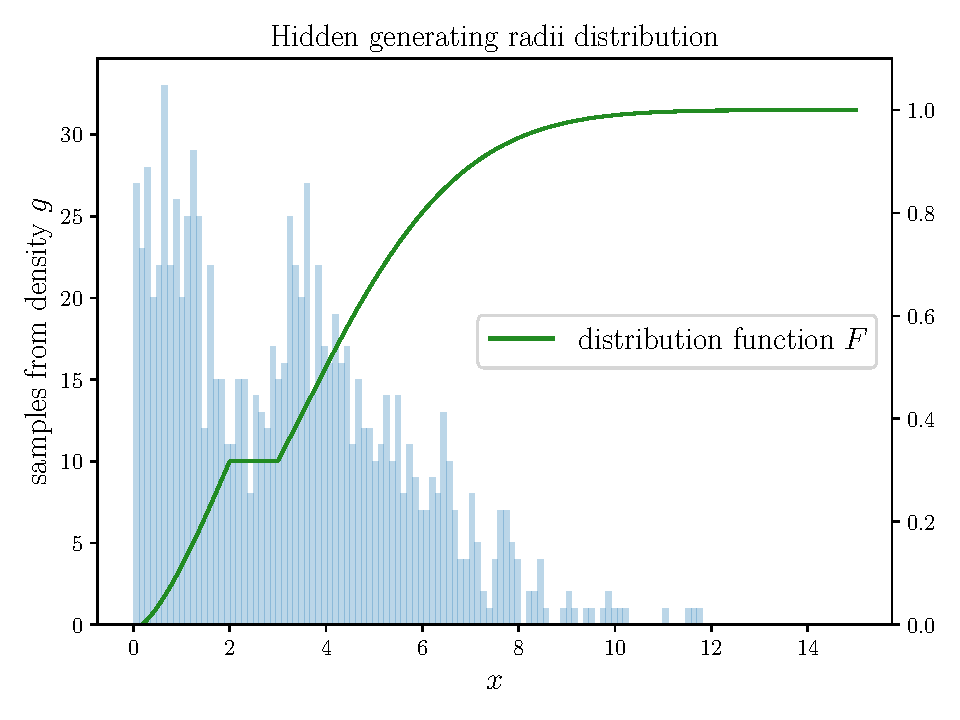
\includegraphics[width=6.4cm]{./img/cdf_truth.pdf}
        \label{fig:image11}
    \end{minipage}
    \hfill
    \begin{minipage}[b]{0.45\textwidth} % Adjust the width as needed
        \centering
        \raisebox{3.1cm}{ % Adjust the value here to move the formula up
        \resizebox{\columnwidth}{!}{%
            \begin{minipage}{\textwidth}
                \begin{align*}
                    &F(x) = \begin{cases}
                        1 - e^{-x^2/20}, & 0 \leq x < 2 \\
                        1 - e^{-1/5}, & x \in [2,3] \\
                        1 - e^{-(x-1)^2/20}, & x > 3
                    \end{cases}
                    \\
                    &g_{\scriptscriptstyle{V}}(x) = \frac{1}{2m_0} \int_{x}^{M} \frac{s e^{-\frac{s^2}{10}} \ind_{[0,2]}(s)}{10\sqrt{s - x}} \, ds \\
                    &\hspace{-0.2cm}+ \frac{1}{2m_0} \int_{x}^{M} \frac{(s-1)e^{-\frac{(s-1)^2}{20}} \ind_{[3,M]}(s)} {10\sqrt{s - x}} \, ds
                \end{align*}
            \end{minipage}}
        }
    \end{minipage}
    \vspace{-0.8cm} % Adjust the value here to decrease the space
    \caption{Underlying cdf $F^*$ and in light blue a histogram of a sample of size $1000$ from $g$.}\label{img: cdf1}
    \vspace{-0.5cm}
    \label{fig:both_images1}
\end{figure}

  
In Figure \ref{img: histograms}, we observe that the distributions of $\sqrt{n} (V^{(\ubar{x},\bar{x})}_n(x)-V(x) )$ and $\sqrt{n} (\hat{V}_n(x)-V(x) )$ closely resemble each other. Moreover, we observe a strong resemblance not only between the estimators but also between their respective limiting distributions, $L_x$ and $N(0,\sigma^2_{\ubar{x},\bar{x}})$. However, the violin plot with the standard percentiles, the second histogram with $\sqrt{n}(\hat{V}_n(x) - V^{(\ubar{x},\bar{x})}_n(x))$ and $W$ and Table \ref{tab: 1} indicate that the variance of $\hat{V}_n(x)$ is slightly bigger than the one of $V^{(\ubar{x},\bar{x})}_n(x)$. 

\begin{figure}[htbp]
    \centering
    \vspace{-0.1cm} 
    \begin{minipage}[b]{0.45\textwidth} % Adjust the width as needed
        \centering
        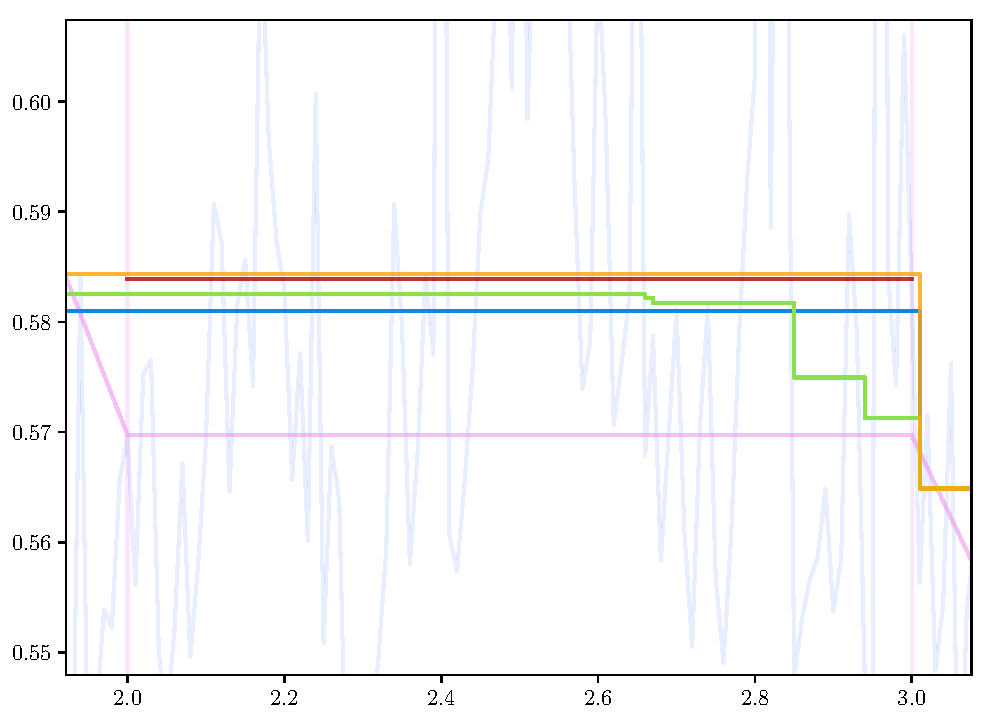
\includegraphics[width = 6.8cm]{img/estimators.pdf}
        \label{fig:image1}
    \end{minipage}
    \hfill
    \begin{minipage}[b]{0.45\textwidth} % Adjust the width as needed
        \centering
        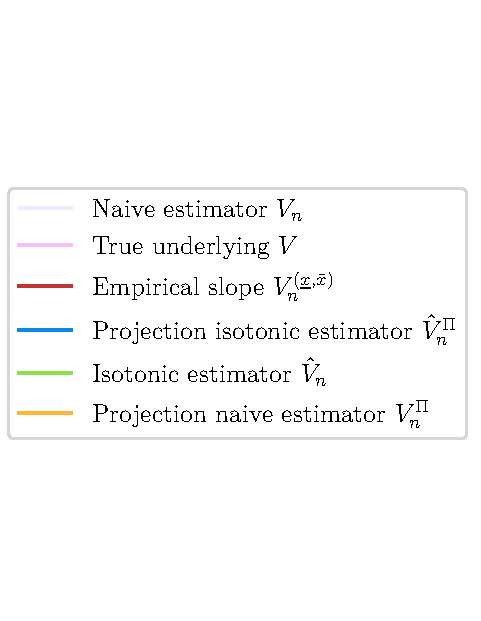
\includegraphics[width = 4.3cm]{img/label_estimators.pdf}
        \label{fig:image2}
    \end{minipage}
    \vspace{-0.6cm} % Adjust the value here to decrease the space
    \caption{All estimators and the true function $V$, which is constant on $[2,3]$, for a sample of size $n=300$.}\label{img: difference all estimators}
    \vspace{-0.1cm}
    \label{fig:both_images}
\end{figure}


The values in Table \ref{tab: 1} were computed using varying sample size $n$ from $g$ as indicated, with $2000$ samples from  $\hat{V}_n(x)$ and $V^{(\ubar{x},\bar{x})}_n(x)$. All the Kernel Density Estimator plots were computed using Scott's rule (where the bin size $h \sim 3.5 \hat{\sigma} n^{-1/3}$) for the chosen bandwidth. For $W$ and $L_x$, $20000$ samples were used.  Taken together, the simulation study confirms the theoretical findings of Theorem \ref{thm: distrib flat F at x total} and \ref{thm: LAM 1}: the informed estimators are efficient and not asymptotically equivalent to the IIE. However, the empirical performances of $V_n^{(\ubar{x},\bar{x})}$ and $\hat{V}_n$ show a high degree of proximity in the estimation scenario where the underlying function $V$ is constant on an interval. Even if $\hat{V}_n$ is used in cases where it is indeed true that $V$ is constant within an interval, the incurred loss appears to be small.


\begin{figure}[H]
    \centering
    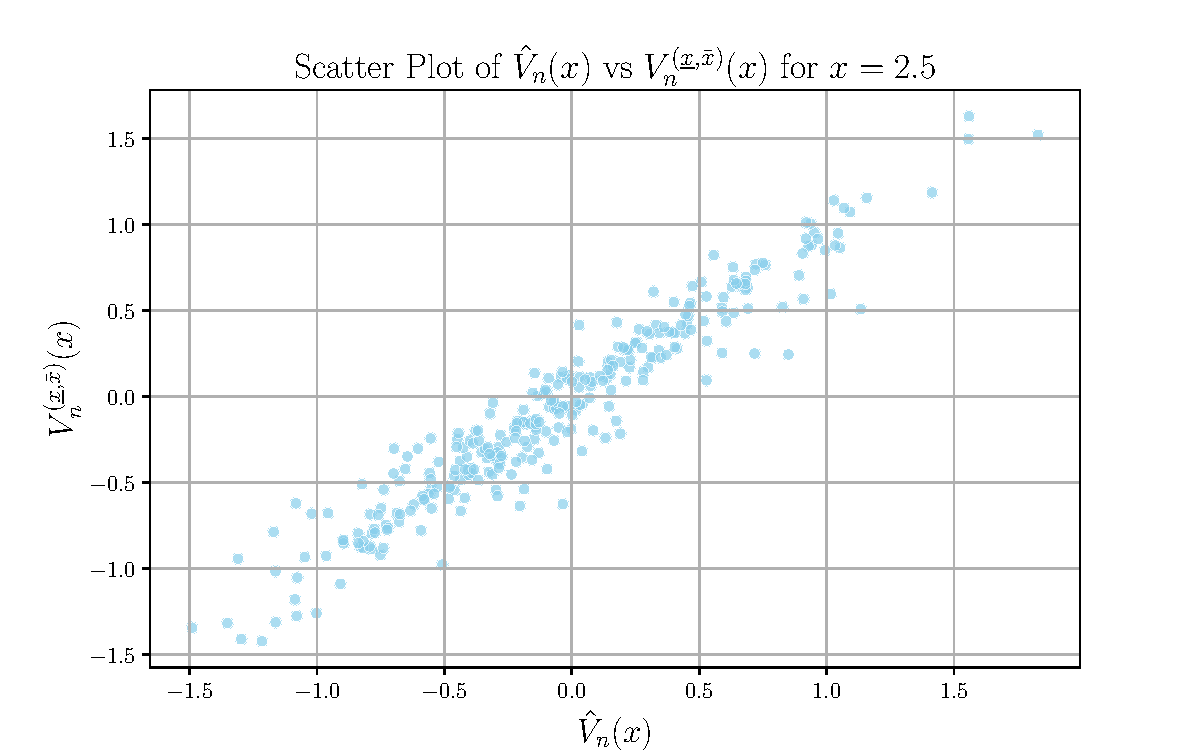
\includegraphics[width=6.5cm]{img/scatterplot1.pdf}
    \hspace{-0.8cm}
    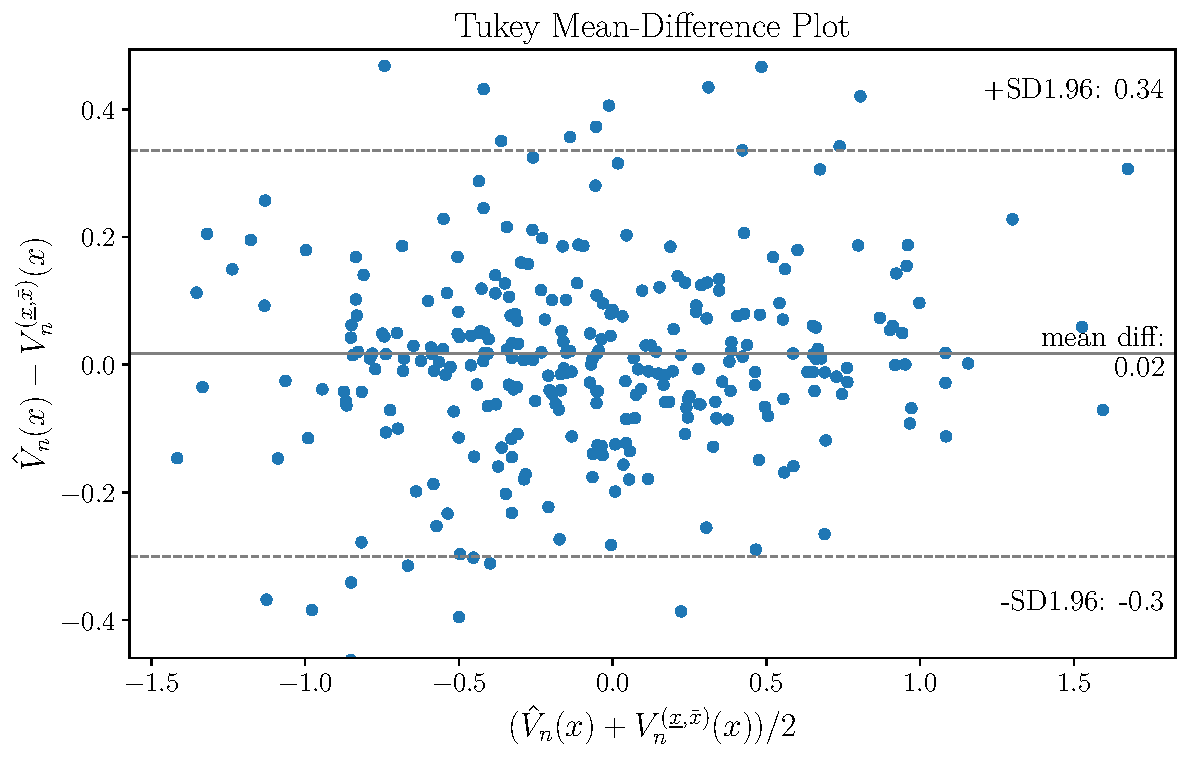
\includegraphics[width=6cm]{img/tukey1.pdf}
    \setlength{\belowcaptionskip}{-6pt}
    \caption{Scatter and Tukey mean-difference plots for $n=1000$ and $300$ repetitions of $\hat{V}_n$ and $V^{(\underline{x},\overline{x})}_n.$}\label{img: scatter + tuckey}
  \end{figure}
\begin{figure}[H]
    \centering
    \vspace{-0.2cm}
    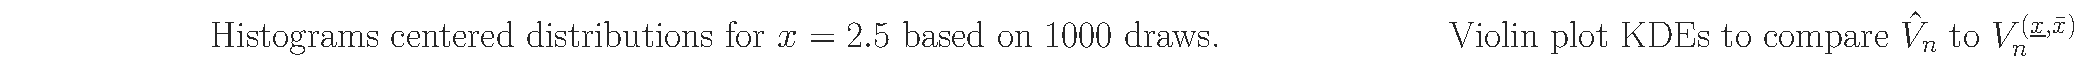
\includegraphics[width=12.1cm]{img/title_histo.pdf}
    \vspace{-0.05cm} 
    
    \begin{minipage}[b]{\linewidth}
      \centering
      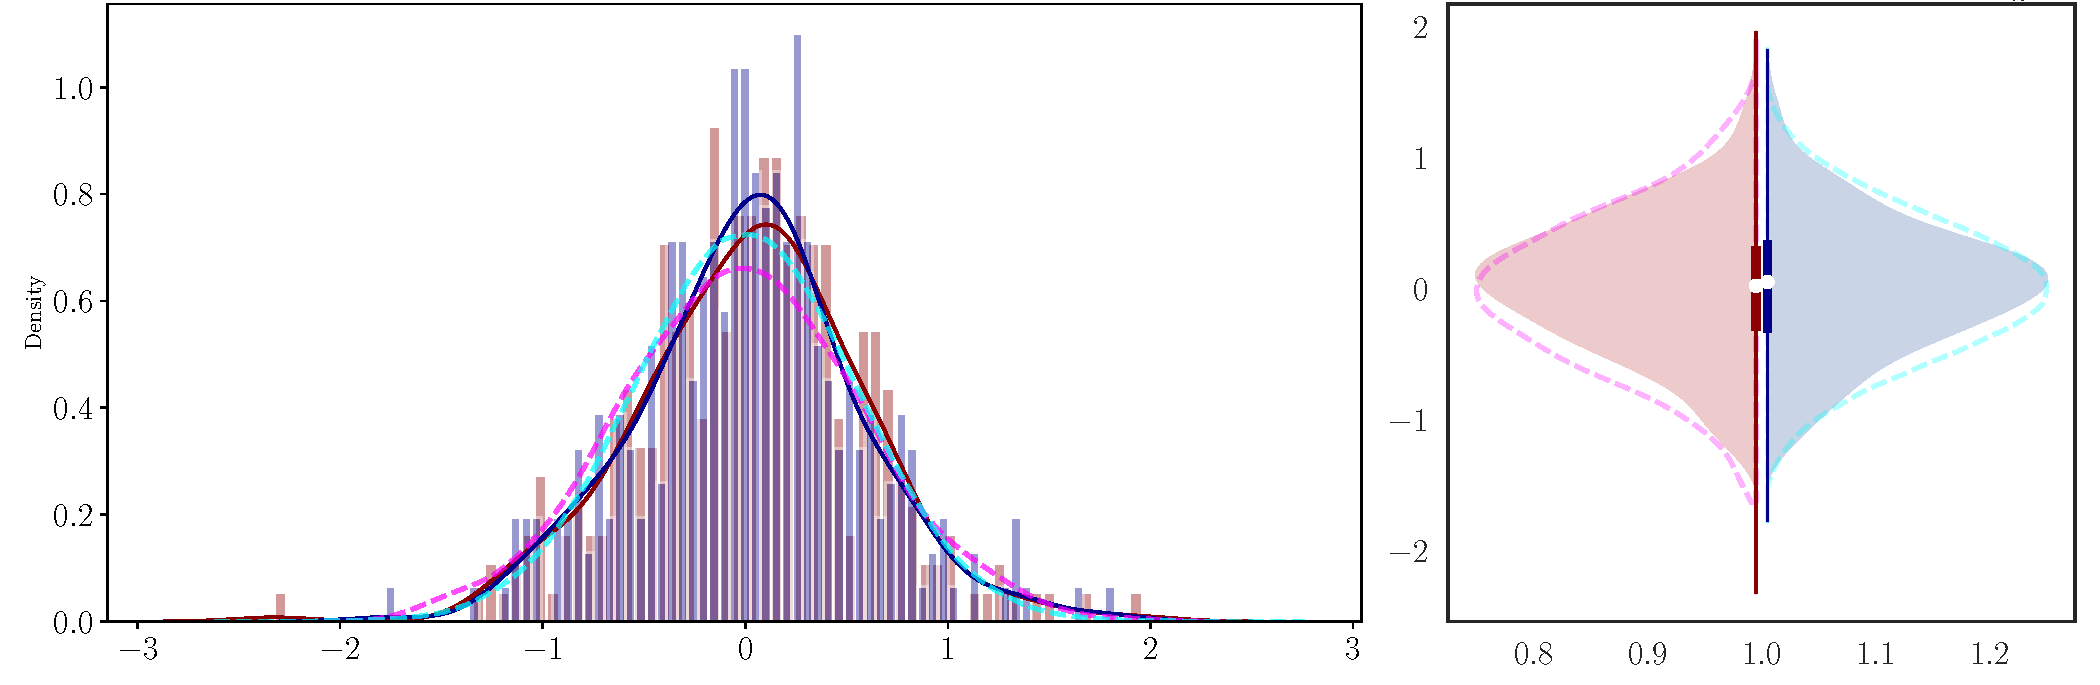
\includegraphics[width=12.1cm]{img/1000_3cropped1.pdf}
    \end{minipage}
  
  \end{figure}
  \begin{figure}[H]
      \centering
      \begin{minipage}[b]{0.45\textwidth} % Adjust the width as needed
          \centering
          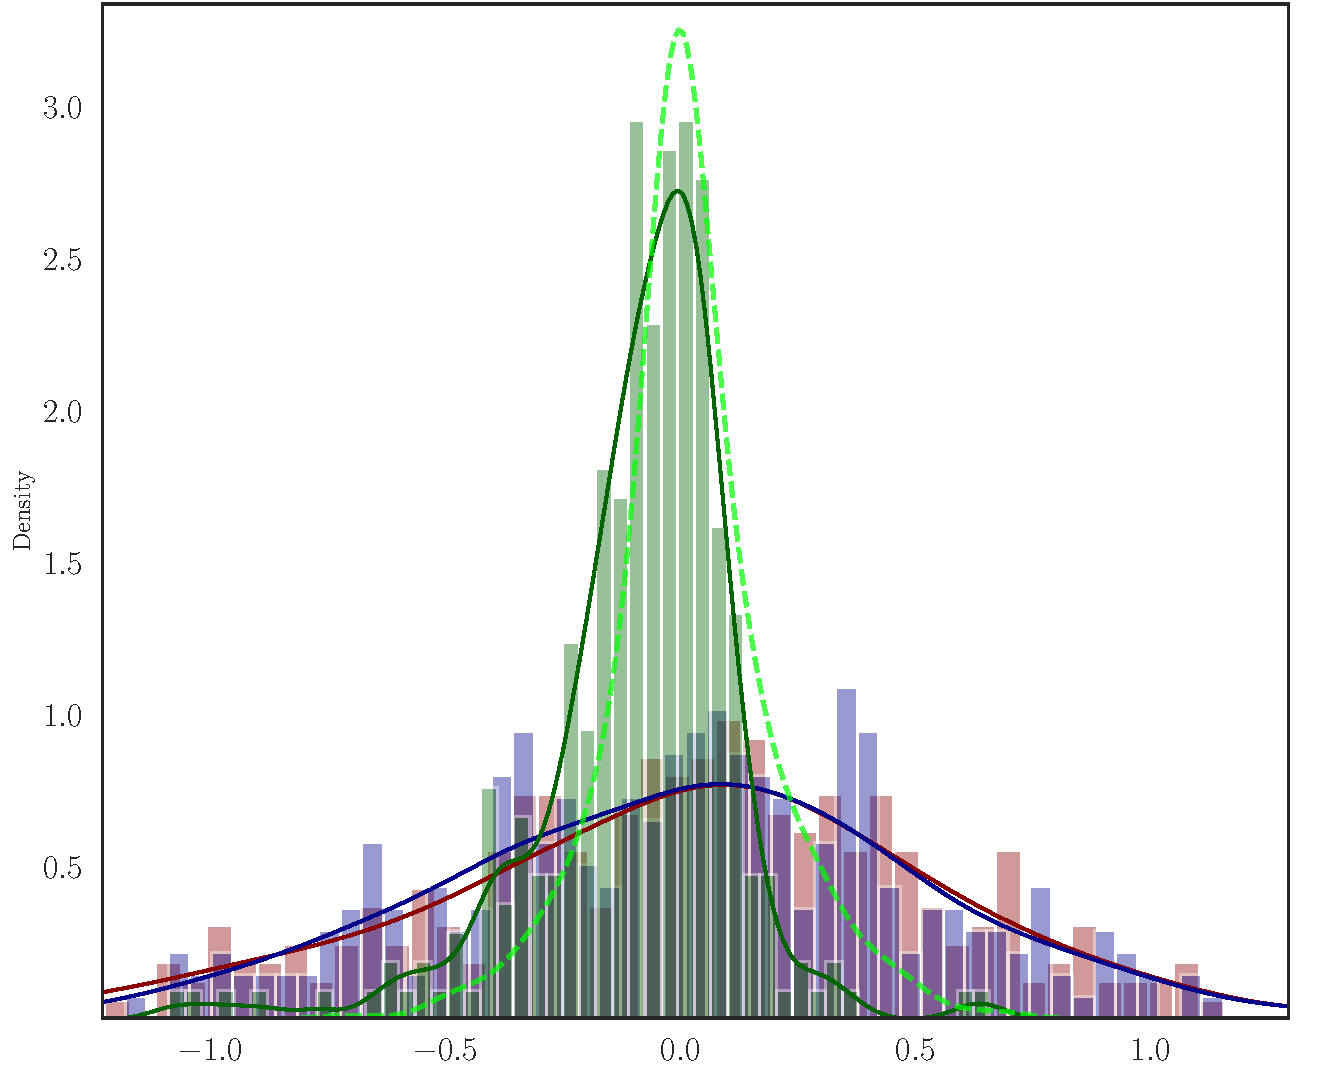
\includegraphics[width=7.2cm]{img/W52cropped.pdf}
          %\caption{First image}\label{fig:image1}
      \end{minipage}
      \hspace{0.8cm}
      \begin{minipage}[b]{0.45\textwidth} % Adjust the width as needed
          \centering
          \raisebox{2.5cm}{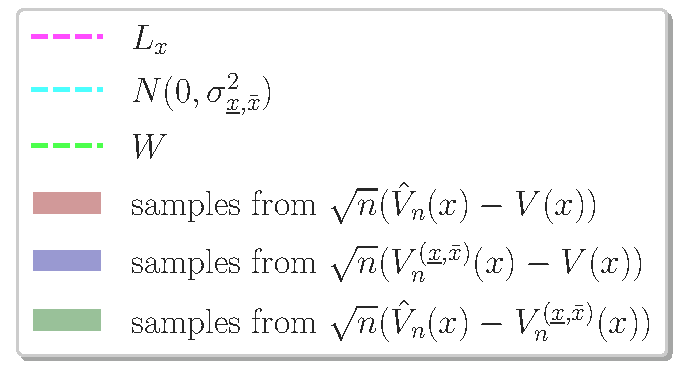
\includegraphics[width=4.2cm]{img/labelextracthisto.pdf}}
          %\caption{Second image}\label{fig:image2}
      \end{minipage}
      \caption{Based on $1000$ samples from $g$, centered and rescaled histograms based on $300$ repetitions, $V^{(\underline{x},\overline{x})}_n$ and their difference compared with respective limiting distributions $L_x$, $N(0,\sigma^2_{\underline{x},\overline{x}}) $ and $W$.}\label{img: histograms}
  \end{figure}




\begin{table}[H]
    \centering
    \resizebox{\columnwidth}{!}{%
    \begin{tabular}{|c|c c c c c||c|c|}
        \hline
         $n$ & 100 & 200 & 400 & 1000 & 2000  &  & limit \\
        \hline
         $\sqrt{n}(V^{(\ubar{x},\bar{x})}_n-V )(x)$ & 0.5441 & 0.5439 & 0.5465 & 0.5467 & 0.5464 & $N(0,\sigma^2_{\ubar{x},\bar{x}})$ & 0.5466 \\
        \hline
         $\sqrt{n} (\hat{V}_n-V)(x)$ & 0.5537 &  0.5592 & 0.5627 & 0.5664 & 0.5697  & $L_x$ & 0.5703 \\
        \hline
    \end{tabular}
    }
    \caption{Standard deviations}
    \label{tab: 1}
\end{table}

\vspace{-1cm}
\subsection{Conclusion}
We conclude by stressing the fact that the local asymptotically minimax variance in Theorem \ref{thm: LAM 1} coincides with the one obtained in Theorem \ref{thm: distrib flat F at x total 2}. This shows that in the setting in which $V$ is constant on $[\ubar{x},\bar{x}]$, for $\ubar{x} < \bar{x}$, the informed estimators are asymptotically efficient, whereas the isotonic inverse estimator is not, as it is clearly shown by Theorem \ref{thm: LAM 1}. However, we conjecture that the isotonic estimator remains asymptotically efficient in the situations in which the boundary points $\ubar{x},\bar{x}$ are allowed to converge to $x$ at an arbitrarily polynomial rate (or slower). In this case, the rate of convergence drops to $\sqrt{n/\log{(\bar{x}-\ubar{x})^{-1}}}$. 

From a practical point of view, both the results of the current section and Theorems \ref{thm: distrib flat F at x}-\ref{thm: normality Holder} are difficult to use to obtain confidence bands, as they require estimating the density \( g \), either at $x$ or globally to compute $\sigma^2_{\ubar{x},\bar{x}}$ or to compute the covariance structure of the limiting Gaussian process. We envision Theorems \ref{thm: distrib flat F at x}-\ref{thm: normality Holder} and the asymptotic results of the current section as the theoretical foundation, while the practical computation of confidence bands may be better addressed through bootstrap methods. A potential direction for further research would be proving formally why the bootstrap works. We believe that a formal justification would combine our theoretical results with the techniques used in \cite{19} (which already shows consistency of the bootstrap for $\gamma =1$ in the limiting variance of Theorem \ref{thm: distrib flat F at x}). 

Another potential direction for further investigation is whether the IIE is efficient in the setting in which there exists an interval of constancy for $V$ but the boundary points $\ubar{x},\bar{x}$ are unknown. However, the definition and assessment of \textit{efficiency} in this context are unclear. For practical purposes, if the boundary points $\ubar{x},\bar{x}$ are unknown, the IIE remains the state-of-art as it behaves very closely to the efficient estimator and in the $\sqrt{n / \log{n}}$ rate setting is efficient and adaptive to the level of smoothness of $V$.


\section{Appendix}\label{sec: appendix chapter2}  % Use * to avoid automatic numbering

\subsection{Proofs of complemental statements for Theorem \ref{thm: normality Holder}.}\label{subsec: proofs lemmas thm normality holder}%% if no title is needed, leave empty \section*{}.
First we provide some proofs about the fundamental behavior of the covariance structure of the process $Z_n(t)$. We start by showing the case of the variance and we will proceed by giving a proof along the same lines of \eqref{eq: covariance structure final}. We will use several times how samples of $Z$ with density $g$ (see \eqref{eq: density of the observations}) are obtained in Wicksell's problem. First, note that the observable radii in the cross sections cannot exceed the radii of the associated sphere; the spheres with bigger radius are more likely to be sampled. Thus the distribution of the squared radii of the spheres actually cut is not $F^*$ but a biased version of it; thus we write $X$ with distribution function $F$ for the squared radius of the spheres actually cut. Since we assume the samples are gathered uniformly, the observed squared circle radius $Z$ is related to $X$ via:
\begin{align}\label{eq: sampling of Z}
    Z = (1-U^2) X = V X, \quad U \sim U[0,1], \quad V \sim \mathrm{Be}(1,1/2)
\end{align}

\begin{lemma}\label{lemma: variance without assum. g}
Fix $x >0$. If $g(x) < \infty$, then:
\begin{align*}
    \ex \left(\sqrt{Z-x} \ind_{\{Z>x\}}-\sqrt{Z-x-\varepsilon} \ind_{\{Z>x+\varepsilon\}}\right)^2 \sim \varepsilon^2 \log \left( \frac{1}{\varepsilon} \right) g (x), \quad \text{as} \quad \varepsilon \downarrow 0.
\end{align*}
\end{lemma}
\begin{proof}
Define $Z_x := Z-x$. The left side is: 
\begin{align*}
\underbrace{\ex Z_x \ind_{\{ Z_x < \varepsilon \}}}_{(1)} + \underbrace{\ex \left(\sqrt{Z_x} - \sqrt{Z_x - \varepsilon} \right)^2 \ind_{\left\{ Z_x > \varepsilon \right\}}}_{(2)}. 
\end{align*}
We start with $(1)$. By making a substitution below with $vX - x = y(X-x)$, which means $1-v = (1-y)\frac{X-x}{X}$, we obtain:
\begin{align*}
   \ex  \, Z_x \ind_{Z_x < \varepsilon}  &\stackrel{\eqref{eq: sampling of Z}}{=} \ex  \left\{ \ind_{X > x} \int_{0 < vX - x < \varepsilon} (vX -x) \frac{\ind_{0<v<1}}{2 \sqrt{1 - v}} \, dv \right\}  \\
    &\: \: = \ex  \left\{ \ind_{X> x} \int_{0}^{\frac{\varepsilon}{X - x} \wedge 1} \frac{y}{2 \sqrt{1-y}} \frac{(X-x)^{3/2}}{\sqrt{X}} \, dy\right\}.
\end{align*}
If we define $y(z) = \int_{0}^{z} \frac{y}{2 \sqrt{1-y}} \, dy$ then the above equals to:
\begin{align*}
    \ex  \left\{  y\left(\frac{\varepsilon}{X - x} \wedge 1 \right) \ind_{X> x} \frac{(X-x)^{3/2}}{\sqrt{X}} \right\}.
\end{align*}
Using: $\int \frac{y}{2 \sqrt{1-y}} \, dy = \frac{(1-y)^{3/2}}{3} - \sqrt{1-y} + c$, we can see that:
\begin{align*}
    y\left(\frac{\varepsilon}{X - x} \wedge 1\right) &= \int_{0}^{\frac{\varepsilon}{X - x} \wedge 1} \frac{y}{2 \sqrt{1-y}} \, dy =  \frac{1}{4} \left( \frac{\varepsilon}{X-x} \right)^2 + O\left( \left( \frac{\varepsilon}{X-x} \right)^3 \right).
\end{align*}
Moreover it is also true $y(z) \leq z^2, \: \: \forall \: z \in (0,1)$. The above proves:
\begin{align}\label{eq: EZa less equal}
\ex \, Z_x \ind_{Z_x < \varepsilon} = O(\varepsilon^2).     
\end{align}
Therefore $(1)$ is negligible. Now we proceed with $(2)$. Using Taylor's theorem with integral form of the remainder we obtain:
\begin{align*}
    &\ex \left( \sqrt{Z_x} - \sqrt{Z_x - \varepsilon} \right)^2 \ind_{\{ Z_x > \varepsilon \}} =  \ex  \int_{0}^{1} \int_{0}^{1} \frac{\varepsilon}{2 \sqrt{Z_x - \varepsilon s}} \frac{\varepsilon}{2 \sqrt{Z_x - \varepsilon t}} \, ds \, dt \, \ind_{\{Z_x > \varepsilon \}} \\
    &\stackrel{\eqref{eq: sampling of Z}}{=} \ex  \int_{0}^{1} \int_{0}^{1} \int_{0}^{1} \frac{\varepsilon}{2 \sqrt{vX-x - \varepsilon s}} \frac{\varepsilon}{2 \sqrt{v X - x - \varepsilon t}} \frac{1}{2 \sqrt{1-v}} \ind_{\{vX - x > \varepsilon \}} \, dv \, ds \, dt.
\end{align*}
Now we use again the substitution $vX - x = y(X-x)$ which implies $1-v = (1-y) \frac{X-x}{X}$ and $y(\varepsilon,s,t) = \int_{\varepsilon}^{1} \frac{1}{\sqrt{y - \varepsilon s}} \frac{1}{\sqrt{y - \varepsilon t}} \frac{1}{\sqrt{1-y}} \, dy$ to obtain:
\begin{align*}
    &= \frac{\varepsilon^2}{8} \ex  \int_{0}^{1} \int_{0}^{1} \int_{0}^{1} \frac{1}{\sqrt{y - \frac{\varepsilon s}{X-x}}} \frac{1}{\sqrt{y - \frac{\varepsilon t}{X-x}}} \frac{1}{ \sqrt{1-y}} \frac{\ind_{\{y(X - x) > \varepsilon \}}}{\sqrt{X-x} \sqrt{X}} \, dy \, ds \, dt \\
    &= \frac{\varepsilon^2}{8} \ex  \int_{0}^{1} \int_{0}^{1} y\left( \frac{\varepsilon}{X-x},s,t \right) \frac{\ind_{\{X - x > \varepsilon \}}}{\sqrt{X-x} \sqrt{X}} \, ds \, dt.
\end{align*}
Now we show the two following relations $\forall \: 0 < \varepsilon,s,t < 1$:
\begin{align}
    &y(\varepsilon,s,t) \sim \log{\frac{1}{\varepsilon}} - \frac{1}{2}\log{\log{\frac{1}{\varepsilon}}} + O(1) \quad \text{as} \: \varepsilon \downarrow 0 \label{eq: relations on y} \\
    & y(\varepsilon,s,t) \leq \left( \log{\frac{1}{\varepsilon}} + \log{\frac{e^2}{1 - s \vee t}}\right) \frac{1}{\sqrt{1 - s \vee t}} + 1. \label{eq: relations on y 2}
\end{align}
From this it will follow that:
\begin{align}\label{eq: essential second moment rel variance}
    \ex \left( \sqrt{Z_x} - \sqrt{Z_x - \varepsilon} \right)^2 \ind_{\{ Z_x > \varepsilon \}} \sim \frac{\varepsilon^2}{4} g(x) \log{\frac{1}{\varepsilon}}. 
\end{align}
Fix $\varepsilon < b < 1$, then we can split the integral in the definition of $y(\varepsilon,s,t)$ into two integrals: one from $\varepsilon$ to $b$ and another one from $b$ to $1$. Let us look at the second one:
\begin{align*}
    \int_{b}^1 \frac{(1-y)^{-\frac{1}{2}}}{y \sqrt{y - \varepsilon s}} \frac{y}{\sqrt{y - \varepsilon t}} \, dy \leq& \frac{b}{b - \varepsilon} \int_{b}^1 \frac{1}{y \sqrt{1-y}} \, dy = \frac{b}{b - \varepsilon} 2 \tanh^{-1} (\sqrt{1-b}). 
\end{align*}
Here we used the fact that the mapping $y \mapsto \frac{y}{y-\varepsilon s}$ is decreasing on $[\varepsilon s,1]$, that $\frac{b}{b - \varepsilon s} \leq \frac{b}{b - \varepsilon}$ and $\int \frac{1}{y} \frac{1}{\sqrt{1-y}} \, dy = -2 \tanh^{-1}(\sqrt{1-y}) + c$. This shows that the asymptotic behavior will be determined by the integral between $\varepsilon$ and $b$;
\begin{align*}
    &\bigg| \int_{\varepsilon}^{b} \frac{1}{\sqrt{y - \varepsilon s}} \frac{1}{\sqrt{y - \varepsilon t}} \frac{1}{\sqrt{1 - y}} \, dy - \int_{\varepsilon}^{b} \frac{1}{\sqrt{y - \varepsilon s}} \frac{1}{\sqrt{y - \varepsilon t}} \, dy \bigg| \\
    &\quad \quad \quad \leq \int_{\varepsilon}^{b} \frac{1}{\sqrt{y - \varepsilon s}} \frac{1}{\sqrt{y - \varepsilon t}} \, dy \left( \frac{1}{\sqrt{1-b}} -1 \right).
\end{align*}
On the other hand, since:
\begin{align*}
\int_{\varepsilon}^b \frac{1}{y-\varepsilon s \wedge t} \, d y \leqslant \int_{\varepsilon}^b \frac{1}{\sqrt{y-\varepsilon s}} \frac{1}{\sqrt{y-\varepsilon t}} \, d y \leqslant  \int_{\varepsilon}^b \frac{1}{y-\varepsilon s \vee t} \, d y.
\end{align*}
Therefore we have:
\begin{align*}
    \int_{\varepsilon}^{b} \frac{1}{\sqrt{y - \varepsilon s}} \frac{1}{\sqrt{y - \varepsilon t}} \frac{1}{\sqrt{1 - y}} \, dy 
    \begin{cases}
        \leq \log{\left\{ \frac{b - \varepsilon s \vee t}{\varepsilon (1 - s \vee t)} \right\}} \frac{1}{\sqrt{1-b}}, \\ 
        \geq \log{\left\{ \frac{b - \varepsilon s \wedge t}{\varepsilon (1 -  s \wedge t)} \right\}}\left(2 - \frac{1}{\sqrt{1-b}} \right).
    \end{cases}
\end{align*}
Using $b = \frac{1}{\sqrt{\log{\frac{1}{\varepsilon}}}}$ we obtain for fixed $c$: 
\begin{align*}
    \log{\left\{ \frac{1/\sqrt{\log{\frac{1}{\varepsilon}}} - \varepsilon c}{\varepsilon (1-c)} \right\}} &= \log{\left\{ 1 - \varepsilon \sqrt{\log{\frac{1}{\varepsilon}}} c\right\}} + \log{\left\{ \frac{1}{\sqrt{\log{\frac{1}{\varepsilon}}}} \right\}} + \log{\frac{1}{\varepsilon}} + \\ 
    &\quad + \log{\frac{1}{1-c}} \sim \log{\frac{1}{\varepsilon}} - \frac{1}{2} \log{\log{\frac{1}{\varepsilon}}} + O(1), \quad \quad \text{as} \: \: \varepsilon \downarrow 0.
\end{align*}
This proves the first relation \eqref{eq: relations on y}. Now we proceed with relation \eqref{eq: relations on y 2}. Assume $s \leq t$. By performing a substitution $y - \varepsilon t = z (1 - \varepsilon t)$ which means $1 - y = (1 - \varepsilon t)(1 - z)$ we obtain:
\begin{align*}
    y(\varepsilon,s,t) \leq \int_{\varepsilon}^1 \frac{1}{y - \varepsilon t} \frac{1}{\sqrt{1 - y}} \, dy = \frac{1}{\sqrt{1 - \varepsilon t}} \int_{\frac{\varepsilon (1-t)}{1-\varepsilon t}}^{1} \frac{1}{z} \frac{1}{\sqrt{1-z}} \, dz. 
\end{align*}
We used that we can compute the primitive: $\int \frac{1}{y} \frac{1}{\sqrt{1-y}} \, dy = -2 \tanh^{-1}(\sqrt{1-y}) + c$. Therefore:
\begin{align*}
     &\frac{1}{\sqrt{1 - \varepsilon t}}  \int_{\frac{\varepsilon (1-t)}{1-\varepsilon t}}^{1} \frac{1}{z} \frac{1}{\sqrt{1-z}} \, dz = 2 \tanh^{-1}\left( \sqrt{1 - \frac{\varepsilon (1-t)}{1 - \varepsilon t}}\right) \frac{1}{\sqrt{1 - \varepsilon t}}   \\
     & = \frac{1}{\sqrt{1 - \varepsilon t}} \log{\left\{ \frac{1 +  \sqrt{\frac{1 - \varepsilon}{1 - \varepsilon t}} }{ 1 - \sqrt{\frac{1 - \varepsilon}{1 - \varepsilon t}}} \right\}}  = \log{\left\{ \frac{\left(\sqrt{1 - \varepsilon t} + \sqrt{1 - \varepsilon}\right)^2}{\varepsilon - \varepsilon t} \right\}} \frac{1}{\sqrt{1 - \varepsilon t}}  \\
     & \leq \bigg( \log{\frac{1}{\varepsilon}} + \log{\frac{1 - \varepsilon t}{1-t}} + 2\bigg) \frac{1}{\sqrt{1 - \varepsilon t}} \leq \left( \log{\frac{1}{\varepsilon}} + \log{\frac{e^2}{1-t}} \right) \frac{1}{\sqrt{1 - t}} +1.
\end{align*}
And this proves \eqref{eq: relations on y 2}. Now we proceed by using the two relations we just proved. First of all,  \eqref{eq: relations on y} as $\varepsilon \downarrow 0$:
\begin{align*}
    &\frac{y\left( \frac{\varepsilon}{X_x}, s, t \right) \ind_{\{X_x > \varepsilon \}}}{\log{\frac{1}{\varepsilon}}} = \frac{y\left( \frac{\varepsilon}{X_x}, s, t \right) \ind_{\{X_x > \varepsilon \}}}{\log{\frac{X_x}{\varepsilon}}} \cdot \frac{\log{X_x}  + \log{\frac{1}{\varepsilon}}}{\log{\frac{1}{\varepsilon}}} \rightarrow \ind_{\{ X > x\}}
\end{align*}
Now using $\log{xy} \leq \log{x} \ind_{x> 1} + \log{y}$ and \eqref{eq: relations on y 2} we obtain:
\begin{align*}
    \frac{y\left( \frac{\varepsilon}{X-x}, s,t \right) \mathbf{1}_{\{ X-x > \varepsilon\}}}{ \log{\frac{1}{\varepsilon}}} &\leq \frac{\left( \log{\frac{X_x}{\varepsilon}} + \log{\frac{e^2}{1 - s \vee t}} \right) \frac{1}{\sqrt{1 - s \vee t}} + 1}{\log{\frac{1}{\varepsilon}}} \\ 
    &\lesssim \left( \log{X_x} \ind_{X_x > 1} + \log{\frac{e^2}{\sqrt{1 - s \vee t}}}\right) \frac{1}{\sqrt{1 - s \vee t}} + 1.
\end{align*}
Since the idea is to apply the Dominated Convergence Theorem to:
\begin{align*}
    \frac{1}{\log{\frac{1}{\varepsilon}}} \ex  \int_{0}^{1} \int_{0}^{1} y\left( \frac{\varepsilon}{X-x},s,t \right) \frac{1}{2\sqrt{X-x} \sqrt{X}} \ind_{\{X - x > \varepsilon \}} \: ds \: dt,
\end{align*}
we need to verify that all the upper bounds have finite expectations. First $\frac{\log{X_x}\ind_{\{ X_x > 1\}}}{\sqrt{X}} \lesssim 1$ which means:
\begin{align*}
    \int_{0}^{1} \int_{0}^{1} \frac{\log{X_x} \ind_{\{X_x > 1\}} }{\sqrt{X}} \frac{1}{\sqrt{1 - s \vee t}} \, ds \, dt \lesssim 2 \int_{0}^{1} \int_{0}^{t} \frac{1}{\sqrt{1-t}} \, ds \, dt < \infty.
\end{align*}
On the other hand:
\begin{align*}
    &\int_{0}^{1} \int_{0}^{1} \left( \log{\frac{1}{1 - s \vee t}} \right) \frac{1}{\sqrt{1 - s \vee t}} \, ds \, dt \lesssim 2 \int_{0}^{1} \int_{0}^{t} \left( \log{\frac{1}{1 - t}}\right) \frac{1}{\sqrt{1-t}} \, ds \, dt \\
    &\quad \quad = 2 \int_{0}^{1} t \left( \log{\frac{1}{1-t}} \right) \frac{1}{\sqrt{1-t}} \, dt < \infty.
\end{align*}
So by the Dominated Convergence Theorem, if $g(x)= \ex  \frac{1}{2 \sqrt{X-x}} \frac{1}{\sqrt{X}} \ind_{\{X>x \}} < \infty$ we obtain the claim.
\end{proof}

\begin{proof}[\hypertarget{proof of lemma 1}{\textbf{Proof of}} \eqref{eq: covariance structure final}]
Fix $s, t \in I_x$. Take the case $0 \leq s \leq t$. Fix $\mu$; we define the function $\phi(\cdot, \mu)$ as follows:
$$
\phi(z, \mu)=\sqrt{z-x} \, \ind_{[x, \infty)}(z)-\sqrt{z-x-\mu} \, \ind_{[x+\mu, \infty)}(z) .
$$
Using the i.i.d.\ property, we can write:
\begin{align}\label{eq: equation covariance}
\operatorname{Cov}\left(Z_n(s), Z_n(t)\right)= 4 \delta_n^{-2} ( \delta^*_n)^{-2}  n^{-1} \operatorname{Cov}\left(\phi\left(Z, \delta^*_n t\right), \phi\left(Z, \delta^*_n s\right)\right),
\end{align}
where $Z$ has density $g$. 
Since $g(x) < \infty$, we will prove:
\begin{align}\label{eq: covariance phi function new}
\ex  \phi\left(Z, \delta^*_n s\right) \phi\left(Z, \delta^*_n t\right)=- \frac{1}{4}st g(x) (\delta^*_n)^2 \log{\delta^*_n} +O\left((\delta^*_n)^2 \right),
\end{align}
which implies \eqref{eq: covariance structure final} for $\delta_n=n^{-1 / 2} \sqrt{\log n}$ and $\delta^*_n = (\delta_n)^{1/\gamma_x}$. Define $Z_x := Z-x$:
\begin{align*}
    &\ex \left[ \sqrt{Z_x} \ind_{\{Z_x > 0 \}} - \sqrt{Z_x - \delta^*_n t} \ind_{\{Z_x > \delta^*_n t \}} \right] \hspace{-0.1cm} \left[ \sqrt{Z_x} \ind_{\{Z_x > 0 \}} - \sqrt{Z_x - \delta^*_n s} \ind_{\{Z_x > \delta^*_n s \}} \right]\\
    &= \underbrace{\ex  Z_x \ind_{\{ 0 < Z_x < \delta^*_n s\}}}_{(1)} + \underbrace{\ex  \left\{ \sqrt{Z_x} \left(\sqrt{Z_x} - \sqrt{Z_x - \delta^*_n s} \right) \ind_{\{ \delta^*_n s \leq Z_x \leq \delta^*_n t\}}\right\}}_{(2)} + \\
    &\quad + \underbrace{\ex \left\{\left( \sqrt{Z_x} - \sqrt{Z_x - \delta^*_n t} \right) \left( \sqrt{Z_x} - \sqrt{Z_x - \delta^*_n s} \right) \ind_{\{Z_x >  \delta^*_n t \}} \right\}}_{(3)}.
\end{align*}
Let us start with $(1)$. We can use \eqref{eq: EZa less equal} to see that for $\delta^*_n$ going to zero: 
\begin{align*}
    \ex  Z_x \ind_{\{0 < Z_x < \delta^*_n s \}} \leq (\delta^*_n s)^2 \ex  \frac{1}{\sqrt{X-x}} \frac{1}{\sqrt{X}} \ind_{\{ X > x\}} = O((\delta^*_n s)^2).
\end{align*}
This shows that this term is negligible as for the covariance it is multiplied by $4 \delta_n^{-2} ( \delta^*_n)^{-2}  n^{-1} = 4 \frac{1}{\log{n}} ( \delta^*_n)^{-2}$, will be of order $\frac{1}{\log{n}}$ and it will go to zero. \\
Let us continue with $(2)$. First note one can upper bound $(2)$ using Hölder's inequality and notice that by \eqref{eq: essential second moment rel variance} we have:
\begin{align}\label{eq: symmetric case moment squared}
    \ex  \left( \sqrt{Z_x} - \sqrt{Z_x - \delta^*_n s}\right)^2 \ind_{\{ Z_x > \delta^*_n s \}} \sim \frac{(\delta^*_n s)^2}{4} \log{\frac{1}{\delta^*_n s}} g(x).
\end{align}
Which implies that the square root of this term is of the order $O(\delta^*_n \sqrt{\log{\frac{1}{\delta^*_n}}})$. Moreover, notice that by \eqref{eq: EZa less equal}:
\begin{align*}
    \left\{ \ex  Z_x \ind_{\{ \delta^*_n s < Z_x < \delta^*_n t \}} \right\}^{1/2} \leq \left\{ \ex  Z_x \ind_{\{  Z_x > \delta^*_n s \}} \right\}^{1/2} = O(\delta^*_n ).
\end{align*}
All together we obtain that $(2)$ is of the order $O((\delta^*_n)^2 \sqrt{\log{(\delta^*_n})^{-1}})$. This quantity for the covariance structure will be multiplied by $4 \delta_n^{-2} ( \delta^*_n)^{-2}  n^{-1}$, and will be of order $O(\frac{1}{\sqrt{\log{n}}})$ thus it will go to zero because $\sqrt{\log{\frac{1}{\delta^*_n}}} \sim \sqrt{\log{n}}$. \\
Now we argue the order of $(3)$. We argue like in the proof of \eqref{eq: essential second moment rel variance}:
\begin{align*}
    (3) &= (\delta^*_n)^2 st \ex  \int_{0}^{1} \int_{0}^{1} \frac{1}{2 \sqrt{Z_x - \delta^*_n s p}} \frac{1}{2 \sqrt{Z_x - \delta^*_n t q}} \, dp \,dq \: \ind_{\{Z_x > \delta^*_n t\}} \\
    &=  \ex  \int_{0}^{1} \int_{0}^{1} \int_{0}^{1} \frac{(\delta^*_n)^2 st}{2 \sqrt{vX-x - \delta^*_n s p}} \frac{\ind_{\{vX - x > \delta^*_n t\}}}{2 \sqrt{v X - x - \delta^*_n t q}} \frac{1}{2 \sqrt{1-v}} \, dv \, dp \, dq.
\end{align*}
Now we use again the substitution $vX - x = y(X-x)$ which implies $1-v = (1-y) \frac{X-x}{X}$ and $y(\delta^*_n,s,t) = \int_{\delta^*_n}^{1} \frac{1}{\sqrt{y - \delta^*_n s}} \frac{1}{\sqrt{y - \delta^*_n t}} \frac{1}{\sqrt{1-y}} dy$ to obtain:
\begin{align*}
    &=\ex  \int_{0}^{1} \int_{0}^{1} \int_{0}^{1} \frac{(\delta^*_n)^2 st}{8 \sqrt{y - \frac{\delta^*_n t}{X-x} q}} \frac{\ind_{\{y(X - x) > \delta^*_n t\}}}{ \sqrt{y - \frac{\delta^*_n s}{X-x} p}} \frac{1}{ \sqrt{1-y}} \frac{1}{\sqrt{X-x} \sqrt{X}} \, dy \, dp \, dq \\
    &= \frac{(\delta^*_n)^2}{8} st \ex  \int_{0}^{1} \int_{0}^{1} y\left( \frac{\delta^*_n}{X-x},sp,tq \right) \frac{1}{\sqrt{X-x} \sqrt{X}} \ind_{\{X - x > \delta^*_n t \}} \, dp \, dq.
\end{align*}
Then one can obtain the claim by using \eqref{eq: relations on y} and \eqref{eq: relations on y 2}. The reason why we can apply the Dominated Convergence theorem is as in the proof of Lemma \ref{lemma: variance without assum. g}. The cases $s \leq 0 \leq t$ and $s \leq t \leq 0$ can be argued in a similar way.
\end{proof}
\begin{comment}
Now assume instead that $s \leq 0 \leq t$:
\begin{align*}
    &\ex\left[ \sqrt{Z_x} \ind_{\{Z_x > 0 \}} - \sqrt{Z_x - \delta^*_n t} \ind_{\{Z_x > \delta^*_n t \}} \right] \left[ \sqrt{Z_x} \ind_{\{Z_x > 0 \}} - \sqrt{Z_x - \delta^*_n s} \ind_{\{Z_x > \delta^*_n s \}} \right] \\
    &= \underbrace{\ex \left\{ \sqrt{Z_x} \left(\sqrt{Z_x} - \sqrt{Z_x - \delta^*_n s} \right)\ind_{\{ 0 \leq Z_x \leq \delta^*_n t\}}\right\}}_{(1)} + \\
    & \quad \quad \quad \quad \quad \quad \quad + \underbrace{\ex\left\{\left( \sqrt{Z_x} - \sqrt{Z_x - \delta^*_n t} \right) \left( \sqrt{Z_x} - \sqrt{Z_x - \delta^*_n s} \right) \ind_{\{Z_x >  \delta^*_n t \}} \right\}}_{(2)}.
\end{align*}
Now the term $(1)$ is non positive. Therefore we have to make sure it will not go to minus infinity once we multiply it by $4 \delta_n^{-2} ( \delta^*_n)^{-2}  n^{-1} = 4 \frac{1}{\log{n}} ( \delta^*_n)^{-2}$, when we look at the covariance structure. Indeed we can lower bound it using again the same reasoning as above with Hölder's inequality and look at the behavior of:
\begin{align*}
    \ex \left\{\left( \sqrt{Z_x - \delta^*_n s} - \sqrt{Z_x} \right)^2 \ind_{Z_x > 0} \right\} = \ex \left\{\left( \sqrt{Z_x} - \sqrt{Z_x + \delta^*_n s} \right)^2 \ind_{Z_x > - \delta^*_n s} \right\}.
\end{align*}
The behavior of the above expression is determined once again by \eqref{eq: essential second moment rel variance}. Therefore $(1)$ is bounded above by $0$ and from below it is of order $O((\delta^*_n)^2 \sqrt{\log{(\delta^*_n)^{-1}}})$. Therefore we conclude that once we multiply it by $4 \delta_n^{-2} ( \delta^*_n)^{-2}  n^{-1}$ it will converge to zero, just like the symmetric case of \eqref{eq: symmetric case moment squared}.\\
Now we determine the behavior of $(2)$. Using the same reasoning as above, we have:
\begin{align*}
    (2) = \frac{(\delta^*_n)^2}{8} st \ex \int_{0}^{1} \int_{0}^{1} y\left( \frac{\delta^*_n}{X-x},sp,tq \right) \frac{1}{\sqrt{X-x} \sqrt{X}} \ind_{\{X - x > \delta^*_n t \}} dp \: dq,
\end{align*}
where: $y(\varepsilon, ps, tq )= \int_{\varepsilon t}^{1} \frac{1}{\sqrt{y - \varepsilon s p}} \frac{1}{\sqrt{y - \varepsilon tq}} \frac{1}{\sqrt{1-y}} dy $. We show the two following relations $\forall \: 0 < \varepsilon,q,p < 1$ and $s \leq 0 \leq t$:
\begin{align}
    &y(\varepsilon,ps,tq) \sim \log{\frac{1}{\varepsilon}} - \frac{1}{2}\log{\log{\frac{1}{\varepsilon}}} + O(1), \quad \text{as} \: \varepsilon \downarrow 0, \label{eq: relations on y .1} \\
    & y(\varepsilon,ps,tq) \leq \left( \log{\frac{1}{\varepsilon}} + \log{\frac{e^2}{t - p s \vee t q}}\right) \frac{1}{\sqrt{1 - \varepsilon (p s \vee tq)}} + 1. \label{eq: relations on y 2.1}
\end{align}
From this will therefore follow that:
\begin{align*}
    \ex\left( \sqrt{Z_x} - \sqrt{Z_x - \delta^*_n t} \right) \left( \sqrt{Z_x} - \sqrt{Z_x - \delta^*_n s} \right) & \ind_{\{Z_x >  \delta^*_n t \}} \sim \frac{(\delta^*_n)^2}{4} st \: g_{0}(x) \log{\frac{1}{\delta^*_n}}. 
\end{align*}
Fix $t \varepsilon < b < 1$, then we can split the integral in the definition of $y(\varepsilon,ps,tq)$ into two integrals: one from $\varepsilon t$ to $b$ and another one from $b$ to $1$. Let us look at the second one:
\begin{align*}
    \int_{b}^1 \frac{(1-y)^{-\frac{1}{2}}}{y \sqrt{y - \varepsilon sp}} \frac{y}{\sqrt{y - \varepsilon tq}} dy \leq& \frac{b}{b - \varepsilon} \int_{b}^1 \frac{1}{y \sqrt{1-y}} dy = \frac{b}{b - \varepsilon} 2 \tanh^{-1} (\sqrt{1-b}). 
\end{align*}
Here we used the fact that the map $y \mapsto \frac{y}{y-\varepsilon t q}$ is decreasing on $[\varepsilon t,1]$, that $\frac{b}{b - \varepsilon t q} \leq \frac{b}{b - \varepsilon t}$, that for negative $s$ the map $y \mapsto \frac{y}{y-\varepsilon s p }$ is decreasing on $[\varepsilon t,1]$ so $\frac{y}{y-\varepsilon s p } \leq 1$ and that $\int \frac{1}{y} \frac{1}{\sqrt{1-y}} dy = -2 \tanh^{-1}(\sqrt{1-y}) + c$. This shows that the asymptotic behavior will be determined by the integral between $\varepsilon t$ and $b$;
\begin{align*}
    \bigg| \int_{\varepsilon t}^{b} \frac{1}{\sqrt{y - \varepsilon s p}} \frac{1}{\sqrt{y - \varepsilon t q}} \frac{1}{\sqrt{1 - y}} dy &- \int_{\varepsilon t}^{b} \frac{1}{\sqrt{y - \varepsilon s p}} \frac{1}{\sqrt{y - \varepsilon t q}} dy \bigg| \\
    &\leq \int_{\varepsilon t}^{b} \frac{1}{\sqrt{y - \varepsilon s p}} \frac{1}{\sqrt{y - \varepsilon t q}} dy \left( \frac{1}{\sqrt{1-b}} -1 \right).
\end{align*}
On the other hand, since:
\begin{align*}
\int_{\varepsilon t}^b \frac{1}{y-\varepsilon (sp \wedge tq)} d y \leqslant \int_{\varepsilon t}^b \frac{1}{\sqrt{y-\varepsilon s p}} \frac{1}{\sqrt{y-\varepsilon t q}} d y   \leqslant \int_{\varepsilon t}^b \frac{1}{y-\varepsilon (sp \vee tq)} d y.
\end{align*}
Therefore we have:
\begin{align*}
    \int_{\varepsilon t}^{b} \frac{1}{\sqrt{y - \varepsilon s p}} \frac{1}{\sqrt{y - \varepsilon t q}} \frac{1}{\sqrt{1 - y}} dy 
    \begin{cases}
        \leq \log{\left\{ \frac{b-\varepsilon (sp \vee tq)}{\varepsilon(1-sp \vee tq)} \right\}} \frac{1}{\sqrt{1-b}}, \\ 
        \geq \log{\left\{ \frac{b-\varepsilon (sp  \wedge tq)}{\varepsilon(1-sp \wedge tq)} \right\}}\left(2 - \frac{1}{\sqrt{1-b}} \right),
    \end{cases}
\end{align*}
using $b = \frac{1}{\sqrt{\log{\frac{1}{\varepsilon}}}}$ and the same computations as in the proof of Lemma \ref{lemma: variance without assum. g} we obtain for fixed $c$: 
\begin{align*}
    \log{\left\{ \frac{1/\sqrt{\log{\frac{1}{\varepsilon}}} - \varepsilon c}{\varepsilon (1-c)} \right\}} \sim \log{\frac{1}{\varepsilon}} - \frac{1}{2} \log{\log{\frac{1}{\varepsilon}}} + O(1), \quad \quad \text{as} \: \: \varepsilon \downarrow 0.
\end{align*}
And this proves \eqref{eq: relations on y .1}. Now we proceed with the proof of \eqref{eq: relations on y 2.1}. By performing a substitution $y - \varepsilon(ps \vee tq) = z (1 - \varepsilon (ps \vee tq))$ which means $1 - y = (1 - \varepsilon (ps \vee tq))(1 - z)$ we obtain, for $u = \frac{\varepsilon t - \varepsilon (ps \vee tq)}{1-\varepsilon (ps \vee tq)}$:
\begin{align*}
    y(\varepsilon,ps,tq) \leq \int_{\varepsilon t}^1 \frac{1}{y - \varepsilon (ps \vee tq)} \frac{1}{\sqrt{1 - y}} dy = \frac{1}{\sqrt{1 - \varepsilon (ps \vee tq)}} \int_{u}^{1} \frac{1}{z} \frac{1}{\sqrt{1-z}} dz. 
\end{align*}
We now use the fact that we can compute the following primitive: $\int \frac{1}{y} \frac{1}{\sqrt{1-y}} dy = -2 \tanh^{-1}(\sqrt{1-y}) + c$. Thus, for $L = 1/\sqrt{1 - \varepsilon (ps \vee tq)}$ the expression above equals:
\begin{align*} 
     & = 2L\tanh^{-1}\left( \sqrt{1 - \frac{\varepsilon t - \varepsilon (ps \vee tq)}{1-\varepsilon (ps \vee tq)}}\right) = L \log{\left\{ \frac{1 +  \sqrt{\frac{1 - \varepsilon t}{1-\varepsilon (ps \vee tq)}} }{ 1 - \sqrt{\frac{1 - \varepsilon t}{1-\varepsilon (ps \vee tq)}}} \right\}} \\
     &=L \log{\left\{ \frac{\left(\sqrt{1 - \varepsilon (ps \vee tq)} + \sqrt{1 - \varepsilon t}\right)^2}{\varepsilon t - \varepsilon (ps \vee tq)} \right\}} \leq L \bigg( \log{\frac{1}{\varepsilon}} +\log{\frac{1}{t-(ps \vee tq)}} +\\
     & + \log{(1 - \varepsilon (ps \vee tq))} + 2\bigg) \leq \left( \log{\frac{1}{\varepsilon}} + \log{\frac{e^2}{t-(ps \vee tq)}} \right) \frac{1}{\sqrt{1 - \varepsilon(ps \vee tq)}} +1.
\end{align*}
And this proves \eqref{eq: relations on y 2.1}. Finally one can apply the Dominated Convergence Theorem using the same argument used in  Lemma \ref{lemma: variance without assum. g}. The case $s \leq t \leq 0$ can be argued using the same techniques used to argue the previous two cases.
\end{comment}

\begin{proof}[\hypertarget{proof of lemma 2}{\textbf{Proof of}} \eqref{eq: marginal convergence chapter2}]
We verify the Lindeberg condition for $Z_n(1)$. Recall from \eqref{eq: Z_n(1)} the definition of $Z_n(1)$. Then set $Z_n(1) = \sum_{k=1}^{n} (X^n_k - \ex X^n_k)$ and thus $s^2_n = \sum_{k=1}^{n}\mathrm{Var}(X^n_k)$, which on the other hand means:
\begin{align*}
X_k^n = \frac{2\delta_n^{-1}}{n} \frac{\sqrt{Z_k-x} \ind_{[x, \infty)}\left(Z_k\right)-\sqrt{Z_k -x-\delta_n^*} \ind_{\left[x+\delta_n^*, \infty\right)} (Z_k)}{\delta_n^*}.  
\end{align*}
Therefore by \eqref{eq: covariance structure final}: $s_n^2 = \mathrm{Var}\left( Z_n(1)\right)=\frac{1}{2 \gamma_x} g(x) \left(1-\frac{\log \log n}{\log n}\right)+O\left(\frac{1}{\log n}\right)$. We show $\ex  X^n_k = \frac{(\delta^*_n)^{-1} \delta_n^{-1}}{n} O(\delta^*_n) = O(\frac{1}{\sqrt{n \log{n}}})$. It is enough to prove for $\delta^*_n \downarrow 0$:
\begin{align}\label{eq: enough to be shown}
    \int \left\{ \sqrt{z-x} \ind_{[x, \infty)}(z)-\sqrt{z-x-\delta_n^* } \ind_{\left[x+\delta_n^* , \infty\right)}(z) \right\} g (z) d z = O(\delta^*_n).
\end{align}
Let $Z_x := Z -x$ therefore the right-hand side of the above can be written as:
\begin{align*}
& \underbrace{\ex \left[ \sqrt{Z_x} \ind_{\{0 < Z_x < \delta^*_n \}}  \right]}_{=(a)} +\underbrace{\ex \left( \sqrt{Z_x} - \sqrt{Z_x - \delta^*_n} \right) \ind_{\{Z_x > \delta^*_n \}}}_{=(b)}.
\end{align*}
We show $(a) = O(\delta^*_n)$. By using \eqref{eq: sampling of Z} (we denote $X^b$ by $X$ for brevity) and making a substitution below with $vX - x = y(X-x)$, which means $1-v = (1-y)\frac{X-x}{X}$, we obtain:
\begin{align*}
    \ex  \sqrt{Z_x} \ind_{Z_x < \delta^*_n} &= \ex  \left\{ \ind_{X > x} \int_{0 < vX - x < \delta^*_n} \sqrt{vX -x} \frac{\ind_{0<v<1}}{2 \sqrt{1 - v}} \, dv \right\}  \\
    &= \ex  \left\{ \ind_{X> x} \int_{0}^{\frac{\delta^*_n}{X - x} \wedge 1} \frac{\sqrt{y}}{2 \sqrt{1-y}} \frac{(X-x)}{\sqrt{X}} \, dy \right\}.
\end{align*}
For $y(z) = \int_{0}^{z} \frac{\sqrt{y}}{2 \sqrt{1-y}} dy$, the above can be upper bounded for all $\delta^*_n$ small:
\begin{align}\label{eq: equation to upper bound Z_x}
    \ex  \left\{  y\left(\frac{\delta^*_n}{X - x} \wedge 1 \right) \ind_{X> x} \frac{X-x}{\sqrt{X}} \right\} \lesssim \ex  \delta^*_n \frac{1}{\sqrt{X}} \ind_{\{X > x \}} = O(\delta^*_n).
\end{align}
That is because: $\int_{0}^{z} \frac{\sqrt{y}}{2 \sqrt{1-y}} dy = \frac{1}{2} \sin^{-1} (\sqrt{z}) - \frac{1}{2} \sqrt{z(1-z)} \leq z$ for $z \in (0,1)$. Now we proceed with $(b)$. By using again \eqref{eq: sampling of Z} and by making a substitution below with $vX - x = y(X-x)$, which means $1-v = (1-y)\frac{X-x}{X}$, we obtain:
\begin{align*}
& \ex \left(\sqrt{Z_x}-\sqrt{Z_x-\delta^*_n}\right) \ind_{\{Z_x>\delta^*_n\}}=\ex  \int_0^1 \frac{\delta^*_n}{2 \sqrt{Z_x-\delta^*_n s}} \: d s \: \ind_{\{Z_x>\delta^*_n\}} \\
& \quad =  \ex  \int_0^1 \int_0^1 \frac{\delta^*_n}{2 \sqrt{v X-x-\delta^*_n s}} \frac{1}{2 \sqrt{1-v}} \ind_{\{Z_x>\delta^*_n\}} \: d v \: d s\\
& \quad = \frac{1}{4} \ex  \int_0^1 \int_0^1 \frac{\delta^*_n}{\sqrt{y(X-x)-\delta^*_n s}} \frac{1}{\sqrt{1-y}} \frac{\sqrt{X}}{\sqrt{X-x}} \frac{X-x}{X} \: d y \: d s \\
& \quad = \frac{\delta^*_n}{4} \ex  \int_0^1  y\left(\frac{\delta^*_n}{X-x}, s\right) \frac{1}{\sqrt{X}} \ind_{\{X>x+\delta^*_n\}} \: d s,
\end{align*}
where $y(\varepsilon,s) = \int_{\varepsilon}^{1} \frac{1}{\sqrt{y-\varepsilon s}} \frac{1}{\sqrt{1-y}} dy$. For $b \in (\varepsilon,1)$, as done previously, we split the integral between $\varepsilon$ and $b$ and between $b$ and $1$. For the first integral we have:
\begin{align*}
    \bigg| \int_{\varepsilon}^{b} \frac{1}{\sqrt{y - \varepsilon s}} \frac{1}{\sqrt{1 - y}} \, dy - \int_{\varepsilon}^{b} \frac{1}{\sqrt{y - \varepsilon s}} \, dy\bigg| \leq \int_{\varepsilon}^{b} \frac{1}{\sqrt{y - \varepsilon s}} \, dy \left( \frac{1}{\sqrt{1-b}} -1 \right).
\end{align*}
From which we conclude:
\begin{align*}
\int_{\varepsilon}^b \frac{1}{\sqrt{y-\varepsilon s}} \frac{1}{\sqrt{1-y}} \, d y = \left\{\begin{array}{l}
\leq (2 \sqrt{b-\varepsilon s}-2 \sqrt{\varepsilon(1-s)})\left(\frac{1}{\sqrt{1-b}}-1\right), \\
\geq (2 \sqrt{b-\varepsilon s}-2 \sqrt{\varepsilon(1-s)})\left(2-\frac{1}{\sqrt{1-b}}\right).
\end{array}\right.
\end{align*}
For the second integral we have:
\begin{align*}
    \int_{b}^{1} \frac{1}{\sqrt{y-\varepsilon s}} \frac{1}{\sqrt{1-y}} \, dy &\leq \frac{1}{\sqrt{b^2 - b\varepsilon}} \left\{ \sqrt{b(1-b)} - \sin^{-1}(\sqrt{1-b}) \right\}.
\end{align*}
Putting together the above computations, for all $\delta^*_n$ small and $b \sim \sqrt{\frac{1}{\log{\frac{1}{\delta^*_n}}}}$:
\begin{align*}
    &\ex \left(\sqrt{Z_x}-\sqrt{Z_x-\delta^*_n}\right) \ind_{\{Z_x>\delta^*_n\}} \lesssim \delta^*_n \ex  \frac{\ind_{\{X > x + \delta^*_n \}}}{\sqrt{X}} = O(\delta^*_n).
\end{align*}
This proves that \eqref{eq: enough to be shown} is true. 

Let us now look at the indicator $\ind_{\left\{\left|X^n_k-\ex X^n_k\right|>\varepsilon s_n\right\}}$. We look separately at the cases: $ X^n_k-\ex X^n_k > \varepsilon s_n$ and $X^n_k-\ex X^n_k < - \varepsilon s_n$. Using the following facts:
\begin{align*}
    &\sqrt{Z_x} \ind_{\{Z_x > 0 \}} - \sqrt{Z_x - \delta^*_n} \ind_{\{Z_x > \delta^*_n \}} = \sqrt{Z_x} \ind_{\{ 0 < Z_x < \delta^*_n\}} + \Big( \sqrt{Z_x} \: +\\
    &   - \sqrt{Z_x - \delta^*_n} \Big) \ind_{\{Z_x > \delta^*_n \}} \leq \sqrt{\delta^*_n} + \int_{0}^{1} \frac{\delta^*_n \ind_{\{Z_x > \delta^*_n \}}}{2 \sqrt{Z_x - \delta^*_n s}} \, ds \leq \sqrt{\delta^*_n} + \delta^*_n \frac{ \ind_{\{Z_x > \delta^*_n \}}}{2 \sqrt{Z_x - \delta^*_n }}.
\end{align*}
So we can rewrite the set $ \{X^n_k-\ex X^n_k > \varepsilon s_n \}$, using the fact that $\ex X_k^n = O\left( \frac{1}{\sqrt{n \log{n}}} \right)$, and noticing that the last inclusion is valid for all $n$ big enough:
\begin{align*}
    &\left\{ \frac{\sqrt{Z_x} \ind_{\{Z_x > 0 \}} - \sqrt{Z_x - \delta^*_n} \ind_{\{Z_x > \delta^*_n \}}}{ \delta^*_n} > \varepsilon s_n \sqrt{n \log{n}}  + O(1) \right\} \\
    & \quad \subseteq \left\{ \frac{\ind_{\{Z_x > \delta^*_n \}}}{2 \sqrt{Z_x - \delta^*_n}} > \varepsilon s_n \sqrt{n \log{n}} - \frac{1}{\sqrt{\delta^*_n}} + O(1) \right\} \\
    & \quad \subseteq \left\{ Z_x < \frac{\delta^*_n}{4\left( \sqrt{\delta^*_n n \log{n}} \varepsilon s_n - 1 + O(\sqrt{\delta^*_n}) \right)^2} + \delta^*_n \right\}.
\end{align*}
Since $\frac{\delta^*_n}{4\left( \sqrt{\delta^*_n n \log{n}} \varepsilon s_n - 1 + O(\sqrt{\delta^*_n}) \right)^2} \sim \frac{1}{n \log{n}}$, for all $n$ big enough we conclude:
\begin{align*}
    \{X^n_k-\ex X^n_k > \varepsilon s_n \} \subseteq \left\{ Z_x < \frac{1}{n\log{n}} + \delta^*_n \right\} =: A_n.
\end{align*}
Now we see that the set $\{X^n_k-\ex X^n_k < - \varepsilon s_n\}$ is negligible, because the object on the left-hand side in the following expression is nonnegative:
\begin{align*}
   \left\{ \frac{\sqrt{Z_x} \ind_{\{Z_x > 0 \}} - \sqrt{Z_x - \delta^*_n} \ind_{\{Z_x > \delta^*_n \}}}{ \delta^*_n} < - \varepsilon s_n \sqrt{n \log{n}}  + O(1) \right\}.
\end{align*}
Therefore we see that the integral over the set $\left|X^n_k-\ex X^n_k\right|>\varepsilon s_n$ for all $n$ big enough has the same behavior as integrating over the set: $A_n$. Using i.i.d.:
\begin{align*}
\sum_{k=1}^{n} \ex [(X^n_k - \ex X^n_k)^2 \ind_{A_n}] \leq \underbrace{2 n \ex [(X^n_k)^2 \ind_{A_n}]}_{(1)} + \underbrace{2 n (\ex  X^n_k)^2 \pb(A_n)}_{(2)} \rightarrow 0.   
\end{align*}
Since $\ex  X_k^n = O(\frac{1}{\sqrt{n \log{n}}})$ we see immediately that $(2)$ goes to 0. Now we prove that $(1)$ also does. We need to look at the following upper bound:
\begin{align*}
\frac{(\delta^*_n)^{-2}}{\log{n}} \ex  \left[ \left\{ Z_x \ind_{\{Z_x > 0 \}} + (Z_x - \delta^*_n) \ind_{\{Z_x > \delta^*_n \}} \right\} \ind_{A_n} \right] \hspace{-0.05cm} \leq \frac{2(\delta^*_n)^{-2}}{\log{n}} \ex  \left[  Z_x \ind_{\{Z_x > 0 \} \cap A_n} \right]
\end{align*}
From \eqref{eq: EZa less equal}, we recall that: $\ex Z_x \ind_{0 < Z_x < \varepsilon} = O(\varepsilon^2)$ for $\varepsilon \downarrow 0$. We conclude that:
\begin{align*}
    &\frac{(\delta^*_n)^{-2}}{\log{n}} \ex  \left[  Z_x \ind_{\{0 < Z_x < \delta^*_n + \frac{1}{n \log{n}} \}} \right] \sim \frac{1}{\log{n}} \left( \frac{n}{\log{n}} \right)^{\frac{1}{\gamma_x}} \left( \left(\frac{\log{n}}{n} \right)^{\frac{1}{2\gamma_x}} + \frac{1}{n \log{n}} \right)^2 \sim \\
    & \quad \sim \frac{1}{\log{n}} + \frac{1}{\log{n}} \left(\frac{n}{\log{n}} \right)^{1/2\gamma_x} \frac{1}{n \log{n}} + \frac{1}{\log{n}}
 \left( \frac{n}{\log{n}} \right)^{1/\gamma_x} \frac{1}{n^2 \log^2{n}} \rightarrow 0.
 \end{align*}
 For $\gamma_x> \frac{1}{2}$. Therefore the Lindeberg condition is satisfied for $Z_n(1)$.
\end{proof}

\begin{proof}[\hypertarget{proof of lemma 3}{\textbf{Proof of}} \eqref{eq: stochastic boundedness seq argmax}]
We start with the class of functions $h_\theta:[0, \infty) \rightarrow \mathbb{R}$:
\begin{align*}
\mathscr{H}= \bigg\{h_\theta \: : \: h_\theta(z) =& \: 2 \sqrt{z-x} \ind_{[x, \infty)}(z)-2 \sqrt{z-\theta} \ind_{[\theta, \infty)}(z)-a_0(x-\theta), \theta \geq 0 \bigg\}
\end{align*}
and, for $\eta>0$, its subclass $ \mathscr{H}_\eta=\left\{h_\theta \in \mathscr{H}:|\theta-x| \leq \eta\right\}$.
In \cite{1}, they show that the envelope of $\mathscr{H}_\eta$, $H_\eta(z)=2\left(\sqrt{z-x} \ind_{[x, \infty)}(z)-\sqrt{z-x-\eta} \ind_{[x-\eta, \infty)}(z)\right)+a_0 \eta$, satisfies for all $\eta$ small (cf.\ (11) in \cite{1}):
\begin{align}\label{eq: bound on envelope}
\int H_\eta^2(z) g(z) \, d z \leq-2 g(x) \eta^2 \log \eta.    
\end{align}
The first thing that needs to be proved is that for $|\theta -x|$ small, we have:
\begin{align*}
    \int  h_\theta(z) - h_x (z) \, d G(z) \lesssim - |\theta - x|^{\gamma_x+ 1}.
\end{align*}
Using a Taylor expansion for $\int h_\theta(z) d G(z)$ around $x$ (note $h_x(z) = 0$), we get, using the definition of $U$: $U(x)=\frac{\pi}{2 m_0} \int_0^x(1-F(y)) \, d y =\int_0^x V(y) \, d y$, that there exists $\eta_0 > 0$ such that:
\begin{align*}
&\int h_\theta(z) \, d G(z) = 2 \int \sqrt{z-x} \ind_{[x,\infty)}(z) -  \sqrt{z-\theta} \ind_{[\theta,\infty)}(z) \, dG(z)  - V(x) (\theta-x) \\ 
&= U(x) - U(\theta) - V(x)(x-\theta) \stackrel{(T)}{=} \frac{(\theta-x)\pi}{2 m_0} \int_{0}^{1} F(x + u(\theta-x)) -F(x) \, du  \\
&\stackrel{\text{\eqref{eq: condition roughness intro}}}{=}-\frac{\pi}{2 m_0} |\theta - x|^{\gamma_x+ 1}(K_x + o(1)),
\end{align*}
for all $\theta$ with $|\theta-x|<\eta_0$ and for some constant $K>0$. Note that here we used the same reasoning as in \eqref{eq: reasoning asympt holder} and we also used assumption \eqref{eq: condition roughness intro}. 

Now we show the weak consistency of $T_n\left(a_0 + \delta_n a\right)$ for $x=V^{-1}\left(a_0\right)$. This will follow from Theorem 3, Theorem 4 in \cite{1} and the switch relation \eqref{eq: switch relation}. In other words we prove: $\forall \: \varepsilon >0$ then $\pb\left(\left|T_n\left(a_0 + \delta_n a \right)-x\right| > \varepsilon  \right) \rightarrow 0$. Indeed using the switch relation and consistency of $\hat{V}_n$ we get:
\begin{align*}
    &\pb\left(\left|T_n\left(a_0 + \delta_n a \right)-x\right| > \varepsilon \right) \\
    & \quad \leq \pb \left( T_n (V(x) + \delta_n a) > \varepsilon + x \right) + \pb \left( T_n (V(x) + \delta_n a) < x - \varepsilon \right) \\
    & \quad = \pb \left( \hat{V}_n (x + \varepsilon) > V(x) + \delta_n a \right) + \pb \left( \hat{V}_n (x - \varepsilon) < V(x) + \delta_n a \right) \longrightarrow 0.
\end{align*}
As by consistency $\hat{V}_n(x + \varepsilon) \rightarrow V(x+\varepsilon)$, $\delta_n \downarrow 0$ and $V$ is strictly decreasing at $x$, it will never be the case that $V (x + \varepsilon) \geq V(x)$, nor $V (x - \varepsilon) \leq V(x)$. Note that $V$ is already decreasing by definition, and it cannot be constant in a neighborhood of $x$, as we would get a contradiction with the fact that $F$ is not constant in a neighborhood of $x$. \\
Now we will proceed by deriving the rate of convergence of $T_n(a_0 + \delta_n a)$ to $x = V^{-1}(a_0)$. We will do it by a standard technique using a peeling argument, combined later with what we showed above. 

First it needs to be proved that $\forall \: \varepsilon > 0$ there exists $ \{M_n\}$ sequence of stochastically bounded random variables and a positive constant $\eta_1$ such that:
\begin{align}\label{eq: relation to be proved}
2&\left|\int\left\{\sqrt{z-x} \ind_{[x, \infty)}(z) - \sqrt{z-\theta} \ind_{[\theta, \infty)}(z)\right\} \, d\left(\mathbb{G}_n-G\right)(z)\right| \\
&\quad \quad \quad \quad \quad \quad \quad \quad \leq \varepsilon|x-\theta|^{\gamma_x+ 1}+(\delta^*_n)^{\gamma_x+1} M_n,
\end{align}
for all $\theta$ with $|\theta-x|<\eta_1$, and $\gamma$ as in assumption \eqref{eq: condition roughness intro}. Remember that $x$ has been fixed and that $\delta_n=n^{-1 / 2} \sqrt{\log n}$, whereas $\delta^*_n = (\delta_n)^{1/\gamma_x}$. Now we proceed with the proof of \eqref{eq: relation to be proved}. Fix $\varepsilon > 0$, and let $\{M_n (\omega) \}$ be the random variable defined omega-wise as the infimum of all positive numbers $\eta$ so that:
\begin{align}\label{eq: equation with epsilon}
\left|\int h_\theta(z) \, d\left(\mathbb{G}_n-G\right)(z ; \omega)\right| \leq \varepsilon|x-\theta|^{\gamma_x+ 1}+(\delta^*_n)^{\gamma_x+ 1} \eta,
\end{align}
holds for all $\theta \in\left[x-\eta_1, x+\eta_1\right]$. If we define, for $n, j \geq 1$,
$$
A(n, j)=\left\{\theta \geq 0:(j-1) \delta^*_n \leq|\theta-x| \leq j \delta^*_n\right\},
$$
we can write, for all $n \geq 1$ and $\nu$ constant:
\begin{align*}
& \pb\left\{M_n>\nu\right\} \leq \\
& \quad \leq \sum_{j=1}^{\eta_1 / \delta^*_n} \pb\left\{\sup _{\theta \in A(n, j)} (\delta^*_n)^{-(\gamma_x+ 1)}\left|\int h_\theta(z) \, d\left(\mathbb{G}_n-G\right)(z)\right|>\varepsilon(j-1)^{\gamma_x+ 1}+\nu\right\} \\
& \quad \leq \sum_{j=1}^{\eta_1 / \delta^*_n} \frac{\ex \left\{\sup _{|\theta-x| \leq j \delta^*_n} (\delta^*_n)^{-2(\gamma_x+ 1)}\left[\int h_\theta(z) \, d\left(\mathbb{G}_n-G\right)(z)\right]^2\right\}}{\left[\varepsilon(j-1)^{\gamma_x+ 1}+\nu\right]^2}. \numberthis \label{eq: equation to max bound}
\end{align*}
By maximal inequality 3.1 (ii) in \cite{12} and relation \eqref{eq: bound on envelope} (with $\eta = \delta^*_n j$), $\exists$ a $C>0$ such that, for each $j \leq \eta_1 / \delta^*_n$ and using that $(\delta^*_n)^{-2(\gamma_x+ 1)} = (\delta^*_n)^{-2} \delta^{-2}_n$:
\begin{align*}
&\ex \bigg\{\sup _{|\theta-x| \leq j \delta^*_n} (\delta^*_n)^{-2(\gamma_x+ 1)}\left[\int h_\theta(z) \, d\left(\mathbb{G}_n-G\right)(z)\right]^2\bigg\}  \\
& \quad = (\delta^*_n)^{-2} \frac{n}{\log{n}} \ex \bigg\{\sup _{|\theta-x| \leq j \delta^*_n} \left[\int h_\theta(z) \, d\left(\mathbb{G}_n-G\right)(z)\right]^2\bigg\}  \\
& \quad \leq (\delta^*_n)^{-2} \frac{J(1)^2}{\log{n}} \left( -2 g(x) j^2 (\delta^*_n)^2\log{(\delta^*_n \cdot j)}\right) =  C g(x) j^2 + O\left( (\log{n})^{-1} \right).
\end{align*}
where $J(1)$ is the uniform entropy integral appearing from the application of the maximal inequality 3.1 (ii) in \cite{12}. We argue that $J(1)$ is finite in the proof of Lemma \ref{lemma: conv weak argmax}. Applying this inequality to \eqref{eq: equation to max bound}, it follows that we can upper bound it by: $\sum_{j=1}^{\eta_1 / \delta^*_n} \frac{C g(x) j^2 + o(1)}{\left[\varepsilon(j-1)^{\gamma_x+ 1}+\nu\right]^2}$,
by choosing $\nu$ sufficiently large, $\pb\left\{M_n>\nu\right\}$ can be made arbitrarily small uniformly in $n$, which proves \eqref{eq: relation to be proved}. 

We are now ready to conclude that $T_n\left(a_0 + \delta_n a \right)$ is a $\delta^*_n$-consistent estimator for $x=V^{-1}\left(a_0\right)$. From the above we know with probability tending to 1, $\left|T_n\left(a_0 + \delta_n a \right)-x\right|<\eta_0 \wedge \eta_1,$
for $n \rightarrow \infty$. If $\left|T_n\left(a_0 + \delta_n a \right)-x\right|<\eta_0 \wedge \eta_1$, take $\varepsilon$ in relation \eqref{eq: equation with epsilon} equal to $\frac{\pi K}{4 m_0}$ and obtain that:
\begin{align*}
0 & =\int h_x(z) \, d \mathbb{G}_n(z) \leq \int h_{T_n\left(a_0 + \delta_n a\right)}(z) \, d \mathbb{G}_n(z) \\
& \leq \int h_{T_n\left(a_0 + \delta_n a \right)}(z) \, d G(z)+\frac{\pi K_x}{4 m_0}\left|x-T_n\left(a_0 + \delta_n a\right)\right|^{\gamma_x+1
} +(\delta^*_n)^{\gamma_x+ 1} M_n \\
& = \left( \frac{\pi K_x}{4 m_0} - \frac{\pi K_x}{2 m_0} + o(1) \right)\left|x-T_n\left(a_0 + \delta_n a \right)\right|^{\gamma_x+1
}+(\delta^*_n)^{\gamma_x+ 1} M_n,
\end{align*}
where the sequence $\{M_n\}$ is stochastically bounded by the above part. This proves that $T_n\left(a_0 + \delta_n a \right)-x=O_p\left(\delta^*_n\right)$ for $n \rightarrow \infty$. 
\end{proof}

\begin{lemma}\label{lemma: finite g if rough 2}
    Condition \eqref{eq: condition roughness 2} implies that $F^*$ is not constant in a neighborhood of  $x$ and that: $ \int_{x}^{\infty} \frac{dF^*(s)}{\sqrt{s - x}}  < \infty.$
\end{lemma}
\begin{proof}
Assume \eqref{eq: condition roughness 2}. Suppose $F^*$ is constant in a neighborhood of  $x$ then the limit in \eqref{eq: condition roughness 2} is zero, a contradiction. From condition \eqref{eq: condition roughness 2}, it follows that we can fix $K > \epsilon > 0$ knowing that there exists $\delta >0$ such that $\forall \: t \in \mathbb{R}^{+} \: : \: t \leq \delta$ then: $(K - \epsilon) t^{\gamma_x} \leq F^*(x + t) - F^*(x) \leq (K+\epsilon) t^{\gamma_x}$. Let us set a grid that goes from $x$ to $x + \delta$ as: $x_0 = x + \delta \geq x_1 \geq ... \geq x$, $x_j = x + 2^{-j} \delta$. It is enough to look at:
\begin{align*}
    &\int_{x}^{x+\delta} \frac{dF^*(s)}{\sqrt{s-x}} \leq \sum_{j=0}^{\infty} \int_{x_{j+1}}^{x_j} \frac{dF^*(s)}{\sqrt{s-x}} \leq \sum_{j=0}^{\infty} \frac{(K+\epsilon)2^{-\gamma_x(j+1)}}{\sqrt{2^{-(j+1)}\delta}} - \sum_{j=0}^{\infty} \frac{(K-\epsilon)2^{-\gamma_xj}}{\sqrt{2^{-(j+1)}\delta}},
\end{align*}
where the last expression is finite as $\gamma_x> \frac{1}{2}$.
\end{proof}
\begin{lemma}\label{lemma: bounded density}
If $F^*$ is locally Hölder continuous of degree $\gamma_x> 1/2$ around $x_0$, then the density of the observations $g$ is bounded and continuous around $x_0$.
\end{lemma}
\begin{proof}
Fix any $z$ in a neighborhood of $x_0$, so that $ \exists \: \eta >0 \, : \, F^*$ is Hölder continuous on $(z- \eta, z+ \eta)$. Set $z_j = z + \eta 2^{-j}$ for $j=0,1,2...$ so that $z_0 = z+\eta \geq z_1 \geq ... \geq z$ and therefore $z_j - z_{j+1} = \eta 2^{-j-1}$. We have (note $m_0 < \infty$ by \eqref{eq: finite first moment chapter2}):
\begin{align*}
    &g (z)m_0 = \int_{z}^{\infty} \frac{1}{\sqrt{x-z}} dF^*(x) = \sum_{j=0}^{\infty} \int_{z_{j+1}}^{z_j} \frac{1}{\sqrt{x-z}} dF^*(x) + \int_{z+\eta}^{\infty} \frac{1}{\sqrt{x-z}} dF^*(x)  \\
    &\leq\sum_{j=0}^{\infty} \frac{(F^*(z_j)-F^*(z_{j+1}))}{\sqrt{z_{j+1}-z}}  + \frac{1}{\sqrt{\eta}} \leq \frac{1}{\sqrt{\eta}} \left( \sum_{j=0}^{\infty} \frac{2^{-\gamma(j+1)}}{2^{-\frac{1}{2}(j+1)}} + 1 \right), 
\end{align*}
where the last expression is $< \infty $ if and only if $\gamma_x> \frac{1}{2}$. Now we know that the function $g$ is bounded around $x_0$. We have to prove that it is continuous. Using the same reasoning as in the previous part we have that:
\begin{align*}
     g (z) & =\frac{1}{m_0} \underbrace{\sum_{j=0}^{\infty} \int_{z_{j+1}}^{z_j} \frac{1}{\sqrt{x-z}} dF^*(x)}_{(1)} + \frac{1}{m_0} \underbrace{\int_{z+\eta}^{\infty} \frac{1}{\sqrt{x-z}} dF^*(x)}_{(2)}.
\end{align*}
Since in the previous part of the proof we have been able to bound $(1)$ with the convergent series independent of $z$: $\sum_{j=0}^{\infty} \frac{2^{-\gamma(j+1)}}{2^{-\frac{1}{2}(j+1)}}$, then the Weierstrass criterion for uniform convergence of series of functions (M-test) yields that the series $(1)$ converges uniformly. Now we need to show that $z \mapsto \int_{z_{j+1}}^{z_j} \frac{1}{\sqrt{x-z}} dF^*(x)$ are continuous $\forall \: j$. We also need to show that $(2)$ is continuous. First of all, notice that the following function: $f(s) = \frac{\ind_{[\eta 2^{-j-1}, \eta 2^{-j}]}(s)}{\sqrt{s}}$, is continuous on the compact set $[\eta 2^{-j-1},\eta 2^{-j}]$, thus uniformly continuous.
By taking $s=x-z$, one can retrieve $\frac{\ind_{[z+ \eta 2^{-j-1}, z + \eta 2^{-j}]} (x)}{\sqrt{x-z}}$. Now take $\delta$ so that whenever $|z_1 - z_2| < \delta$, by uniform continuity we have:
\begin{align*}
    \bigg| \frac{\ind_{[z_1 + \eta 2^{-j-1}, z_1 + \eta 2^{-j}]} (x)}{\sqrt{x-z_1}} - \frac{\ind_{[z_2 +\eta 2^{-j-1}, z_2 +\eta 2^{-j}]} (x)}{\sqrt{x-z_2}} \bigg| < \varepsilon.
\end{align*}
Then we have, using the triangle inequality for integrals:
\begin{align*}
    \bigg| \int \frac{\ind_{[z_1 + \eta 2^{-j-1}, z_1 + \eta 2^{-j}]} (x)}{\sqrt{x-z_1}} - \frac{\ind_{[z_2 + \eta 2^{-j-1}, z_2 + \eta 2^{-j}]} (x)}{\sqrt{x-z_2}} dF^*(x) \bigg| \leq \varepsilon \int dF^*(x) = \varepsilon.
\end{align*}
Finally, $(2)$ is continuous because $\frac{\ind_{[z+\eta,\infty)} (x)}{\sqrt{x-z}} = \frac{\ind_{[\eta,\infty)} (x-z)}{\sqrt{x-z}}$ is uniformly continuous on $[\eta, \infty)$. The Weierstrass M-test together with the uniform limit theorem yield continuity of $g$.
\end{proof}

\hypertarget{proof of continuity argmax holder}{\begin{lemma}\label{lem: continuity argmax holder}}%
For every $a \in \mathbb{R}$, $\pb\bigl(\hat{s}(a)=0\bigr)=0$, where
$\hat{s}(a):=\underset{t\in I_x}{\argmax}\bigl\{tX-\frac{\pi K_x}{2m_0}|t|^{1+\gamma_x}-at\bigr\}$
and $X\sim N\bigl(0,\,g(x)/(2\gamma_x)\bigr)$, $x>0$.
\end{lemma}

\begin{proof}
Set $c:=X-a$ and $\varphi(s):=cs-\frac{\pi K_x}{2m_0}|s|^{1+\gamma_x}$.
Since $\varphi$ is strictly concave on each half-line and $\varphi(s)\to-\infty$
as $|s|\to\infty$, the unique maximiser is
\[
  \hat{s}(a)=\operatorname{sign}(c)\Bigl(\frac{2m_0|c|}{\pi K_x(1+\gamma_x)}\Bigr)^{1/\gamma_x},
\]
a strictly increasing function of $c=X-a\sim N(-a,\,g(x)/(2\gamma_x))$.
Since this normal has no atoms, neither does the law of $\hat{s}(a)$; in
particular $\pb(\hat{s}(a)=0)=0$.  The cdf of the limit is continuous, with
explicit form $\pb(\hat{s}(a)\leq x)=\pb\bigl(c\leq\frac{\pi K_x}{2m_0}(1+\gamma_x)\operatorname{sign}(x)|x|^{\gamma_x}\bigr)$.
\end{proof}

\begin{lemma}\label{lemma: uniform collapse}
Let $x=0$ and assume the conditions of Theorem \ref{thm: normality Holder}. Let $M \geq 1$ and let $\kappa_n \rightarrow 0$ with $\log(1/\kappa_n) = o(\log n)$. Then, as $n \rightarrow \infty$:
\begin{align*}
\sup_{\kappa_n < t \leq M} \left|\frac{Z_n(t)}{t} - Z_n(1)\right| \rightarrow 0 \quad \text{in probability.}
\end{align*}
\end{lemma}
\begin{proof}
For $u>0$ and $z>0$ define:
\begin{align*}
k_u(z) := \frac{\sqrt{z}-\sqrt{z-u}\,\ind_{[u,\infty)}(z)}{u} = \begin{cases} \sqrt{z}/u, & \text{if } z \leq u, \\ \left(\sqrt{z}+\sqrt{z-u}\right)^{-1}, & \text{if } z > u. \end{cases}
\end{align*}
Taking $x=0$ in \eqref{eq: Z_n(1)} we have $Z_n(t)/t = 2\delta_n^{-1}\int k_{\delta^*_n t}(z)\, d(\mathbb{G}_n-G)(z)$, hence:
\begin{align}\label{eq: uniform collapse empirical}
\frac{Z_n(t)}{t} - Z_n(1) = 2\delta_n^{-1}\int \left\{k_{\delta^*_n t}(z) - k_{\delta^*_n}(z)\right\} d(\mathbb{G}_n-G)(z),
\end{align}
and the supremum in the statement is a supremum over the class $\mathscr{K}^M_n := \{k_{\delta^*_n t} - k_{\delta^*_n} : \kappa_n < t \leq M\}$. From the two expressions of $k_u$ and from $\sqrt{z}-\sqrt{z-u} = u/(\sqrt{z}+\sqrt{z-u})$ we get, for all $u,z>0$:
\begin{enumerate}[label=(\alph*)]
\item $0 \leq k_u(z) \leq z^{-1/2}$;
\item if $u \leq z$, then $0 \leq k_u(z) - \frac{1}{2\sqrt{z}} = \frac{u}{2\sqrt{z}(\sqrt{z}+\sqrt{z-u})^2} \leq \frac{u}{2z^{3/2}}$;
\item $u \mapsto k_u(z)$ is continuous, nondecreasing on $(0,z]$ and nonincreasing on $[z,\infty)$.
\end{enumerate}
We now show that the class $\mathscr{K}^M_n$ has envelope:
\begin{align*}
H_n(z) := \begin{cases} \sqrt{z}/(\kappa_n\delta^*_n), & \text{if } z \leq \kappa_n\delta^*_n, \\ z^{-1/2}, & \text{if } \kappa_n\delta^*_n < z \leq 2M\delta^*_n, \\ M\delta^*_n\, z^{-3/2}, & \text{if } z > 2M\delta^*_n. \end{cases}
\end{align*}
For $t \in (\kappa_n, M]$, both $u := \delta^*_n t$ and $v := \delta^*_n$ lie in $[\kappa_n\delta^*_n, M\delta^*_n]$. If $z \leq \kappa_n\delta^*_n$, then $z \leq u \wedge v$ and $k_u(z), k_v(z) \in [0, \sqrt{z}/(\kappa_n\delta^*_n)]$. If $\kappa_n\delta^*_n < z \leq 2M\delta^*_n$ we use (a). If $z > 2M\delta^*_n$, then $u,v \leq z$ and by (b) both $k_u(z)$ and $k_v(z)$ lie in $[\frac{1}{2\sqrt{z}}, \frac{1}{2\sqrt{z}} + \frac{M\delta^*_n}{2z^{3/2}}]$. In all cases $|k_u(z)-k_v(z)| \leq H_n(z)$.

Note that $H_n^2(z) \leq 1/z$ for all $z>0$ and that $\int_0^\infty H_n^2(z)\,dz = \frac{1}{2} + \log\frac{2M}{\kappa_n} + \frac{1}{8}$. Therefore, for every $x>0$, splitting the integral at $x/2$:
\begin{align*}
\int_0^x \frac{H_n^2(z)}{\sqrt{x-z}}\,dz \leq \sqrt{\frac{2}{x}}\int_0^\infty H_n^2(z)\,dz + \frac{2}{x}\int_{x/2}^x \frac{dz}{\sqrt{x-z}} = \sqrt{\frac{2}{x}}\left(\frac{21}{8} + \log\frac{2M}{\kappa_n}\right).
\end{align*}
By \eqref{eq: density of the observations} and Fubini's theorem this yields:
\begin{align}\label{eq: uniform collapse envelope}
\int H_n^2(z)\,g(z)\,dz = \frac{1}{2m_0}\int_0^\infty \int_0^x \frac{H_n^2(z)}{\sqrt{x-z}}\,dz\,dF^*(x) \leq \sqrt{2}\left(\frac{21}{8} + \log\frac{2M}{\kappa_n}\right) g(0),
\end{align}
where $g(0)<\infty$ by \eqref{eq: condition finite g at x chapter2}.

By (c), for fixed $(z,r)$ the set $\{u>0 : k_u(z) > r\}$ is an interval. Hence, given $m$ points $(z_1,r_1),\dots,(z_m,r_m)$, the subgraph of $k_u$ picks out those points whose interval contains $u$; the at most $2m$ endpoints of these intervals split $(0,\infty)$ into at most $4m+1$ pieces on each of which the picked out set is constant. Since $4m+1<2^m$ for $m \geq 5$, the class $\{k_u : u>0\}$ is VC, and so is $\mathscr{K}^M_n$, which is obtained by subtracting the fixed function $k_{\delta^*_n}$; its VC index does not depend on $n$, so the uniform entropy integral $J(1)$ is finite and does not depend on $n$ (as in the proof of Lemma \ref{lemma: conv weak argmax}). By the continuity in (c), the supremum over $\mathscr{K}^M_n$ equals the supremum over rational $t$. Therefore, using \eqref{eq: uniform collapse empirical}, maximal inequality 3.1 (ii) from \cite{12} and \eqref{eq: uniform collapse envelope}, and since $\delta_n^{-2} n^{-1} = (\log n)^{-1}$:
\begin{align*}
\ex \sup_{\kappa_n < t \leq M}\left|\frac{Z_n(t)}{t}-Z_n(1)\right|^2 \lesssim \frac{J(1)^2}{\log n}\int H_n^2(z)\,g(z)\,dz \lesssim J(1)^2 g(0)\, \frac{1+\log(1/\kappa_n)}{\log n} \rightarrow 0,
\end{align*}
because $\log(1/\kappa_n) = o(\log n)$. Markov's inequality concludes the proof.
\end{proof}

\begin{proof}[\hypertarget{proof of lemma weak conv}{\textbf{Proof of Lemma}} \ref{lemma: conv weak argmax}]
Because
\begin{align*}
    U_n(s) := \frac{2}{n} \sum_{i=1}^n \left\{ \sqrt{(Z_i)_{+}} - \sqrt{(Z_i-s)_{+}} \right\}, 
\end{align*}
the stated convergence is equivalent to saying that the class of functions $z \rightarrow \sqrt{(z)_{+}} - \sqrt{(z-s)_{+}}, \: s \geq 0$ is Donsker. From Lemma 2.6.16 in \cite{5}, it follows that the class of functions $\{ z- s \: : \: s \geq 0 \}$ is VC, next by Lemma 2.6.18 (ii) in \cite{5} we see that the class $\{ (z -s)_{+} \: : \: s \geq 0 \}$ is VC. Again by Lemma 2.6.18 (vii), (iv) and (v) in \cite{5} we conclude that the class of functions $\{ \sqrt{(z)_{+}} - \sqrt{(z-s)_{+}} \: : \: s \geq 0 \}$ is VC. Such class has envelope: $0 \leq \sqrt{(z)_{+}} - \sqrt{(z-s)_{+}} \leq \sqrt{(z)_{+}}$. Therefore the class is $P$-Donsker for any $P$ with $\int_{0}^{\infty} z dP(z) < \infty$, which is the case here by assumption \eqref{eq: finite first moment chapter2} with $k = \frac{3}{2}$.
Now we prove that $\mathbb{Z}$ is a Gaussian process with a.s.\ continuous sample paths. Consider:
\begin{align*}
    &\ex \left( \mathbb{Z} (t_j) - \mathbb{Z} (t_i) \right)^2 =  \ex  \bigg|\sqrt{(Z - t_j)_{+}} - \sqrt{(Z - t_i)_{+}} \bigg|^2  \leq |t_j - t_i|.
\end{align*}
Where we use the fact that the square root is Hölder continuous of degree $1/2$. 

Since the intrinsic semimetric $d (s,t) := (\ex \left( \mathbb{Z} (s) - \mathbb{Z} (t) \right)^2)^{1/2} \leq \sqrt{|s-t|}$, we obtain sample path continuity of $\mathbb{Z}$. 

By the very same computation as above, we deduce that $\mathrm{Var}(\mathbb{Z}(t) - \mathbb{Z}(s)) \neq 0$ for $s \neq t$ and since $\mathbb{Z}$ is indexed by a $\sigma$-compact metric space, we obtain from Lemma 2.6 in \cite{12} that the maxima of the sample paths of $\mathbb{Z}$ are a.s.\ unique. Finally the covariance structure of $\mathbb{Z}$ is given by direct computation:
\begin{align*}
    \mathrm{Cov} \left( \mathbb{Z}(t),\mathbb{Z}(s) \right) = \mathrm{Cov} \Big( \sqrt{\smash[b]{(Z)_{+}}} - \sqrt{\smash[b]{(Z_t)_{+}}}, \sqrt{\smash[b]{(Z)_{+}}} - \sqrt{\smash[b]{(Z_s)_{+}}} \Big).
\end{align*}
\end{proof}

\begin{proof}[\hypertarget{proof of lemma conv K^c_n}{\textbf{Proof of}} \eqref{eq: conv K^c_n}]
    Note that:
    \begin{align*}
        \sup_{s \in K^c_n} \left\{ Z_n(s) - \sqrt{n} h_x(s)-as \right\} \leq \sup_{s \geq 0} Z_n(s) - \inf_{\substack{s < \ubar{x}-\varepsilon_n \\ s > \bar{x}+\varepsilon_n}} \left\{ \sqrt{n} h_x(s) + as\right\},
    \end{align*}
    where the first term on the right-hand side is $O_p(1)$ by the convergence given in Lemma \ref{lemma: conv weak argmax}. The second infimum is the minimum over the infima over the intervals $[0, \ubar{x}-c]$, $[\ubar{x}-c, \ubar{x}-\varepsilon_n]$, $[\bar{x}+\varepsilon_n,\bar{x}+1]$ and $[\bar{x}+1, \infty)$ for a constant $\varepsilon_1<c<\ubar{x}$. Because $F^*$ is constant in $[\ubar{x},\bar{x}]$, we have $U(s)-U(x)-V(x)(s-x)= 0$ for $s \in [\ubar{x},\bar{x}]$ and from the concavity of $U$:
    \begin{align*}
        U(s)-U(x)-V(x)(s-x)< 0,  \quad \text{for} \quad s \notin [\ubar{x},\bar{x}]. 
    \end{align*} 
    Again from the fact that $U$ is concave and because $[\ubar{x},\bar{x}]$ is maximal:
    \begin{align*}
        &\forall \: \delta >0, \: \exists \: \eta >0 \: : \: U(s) - U(x) - V(x)(s-x)< -\eta |s-\ubar{x}| \quad \text{for} \quad s < \ubar{x}- \delta,\\
        &\forall \: \delta >0, \: \exists \: \eta >0 \: : \: U(s) - U(x) - V(x)(s-x)< -\eta |s-\bar{x}| \quad \text{for} \quad s > \bar{x}+ \delta.
    \end{align*} 
    Therefore using these three facts stated above we have: on $[\bar{x}+1,\infty)$,
    \begin{align*}
        \sqrt{n} h_x(s) + as \geq \sqrt{n} \eta |s-\bar{x}|- |a|s \gtrsim \sqrt{n} \rightarrow \infty
    \end{align*}
    and on $[\bar{x}+ \varepsilon_n, \bar{x}+1]$,
    \begin{align*}
        \sqrt{n} h_x(s) + as \geq \sqrt{n} h_x(\bar{x}+\varepsilon_n) - |a| \rightarrow \infty
    \end{align*}
    by the construction of $\varepsilon_n$. The other two intervals can be handled similarly.
\end{proof}

\begin{proof}[\hypertarget{proof of lemma conv prob}{\textbf{Proof of}} \eqref{eq: conv prob argmax}]
First note:
\begin{align*}
    0 &\leq \sup_{s \in F \cap K_n} \left\{Z_n(s) - \sqrt{n} h_x(s) -as\right\} - \sup_{s \in F \cap K} \left\{Z_n(s) -as\right\} \\
    & \leq \sup_{s \in F \cap K_n} \left\{Z_n(s) -as\right\} - \sup_{s \in F \cap K} \left\{Z_n(s) -as\right\}
\end{align*}
Define the process:
\begin{align*}
    \widetilde{Z}_n(s) := \begin{cases}{Z_n(s)-as,} & \text { if } s \in [\ubar{x},\bar{x}] \\ Z_n(\ubar{x})-a\ubar{x}, & \text { if } s \in [0,\ubar{x}] \\ Z_n(\bar{x})-a\bar{x}, & \text { if } s \in [\bar{x},\infty) \end{cases}
\end{align*}
because: $\sup_{s \in F \cap K_n} \widetilde{Z}_n(s) = \sup_{s \in F \cap K}  \widetilde{Z}_n(s) = \sup_{s \in F \cap K} \left\{Z_n(s) -as\right\}$, then
\begin{align*}
    &\quad \bigg| \sup_{s \in F \cap K_n} \left\{Z_n(s) -as\right\} - \sup_{s \in F \cap K} \left\{Z_n(s) -as\right\} \bigg| \\
    &= \bigg| \sup_{s \in F \cap K_n} \left\{Z_n(s) -as\right\} - \sup_{s \in F \cap K_n} \widetilde{Z}_n(s) \bigg| \leq \sup_{s \in F \cap K_n} \big| Z_n(s) - as - \widetilde{Z}_n(s) \big| \\
    & \leq \sup_{s \in F \cap K_n \cap [0,\ubar{x}]} \big| Z_n(s) - as - \widetilde{Z}_n(\ubar{x}) \big| \vee \sup_{s \in F \cap K_n \cap [\bar{x},\infty)} \big| Z_n(s) - as - \widetilde{Z}_n(\bar{x}) \big| \rightarrow 0
\end{align*}
where we used the asymptotic equicontinuity of the $Z_n$.
\end{proof}

\begin{proof}[\hypertarget{proof of main thm}{\textbf{Proof of Theorem}} \ref{thm: main thm iso}]
The claim is a consequence of $1 - F(x) = V(x)/V(0)$ and by analogy, we construct the estimator using the adaptive isotonic estimator. Apply Slutsky's Lemma together with Theorem \ref{thm: normality Holder} (cf.\ Corollary 1 in \cite{1}) to get Theorem \ref{thm: main thm iso 1}. To prove Theorem \ref{thm: main thm iso 2}, note that $V(y)=V(0)$ since $F^*$ is constant on $K_0$; it is possible to follow the same steps as in the proof of Theorem \ref{thm: distrib flat F at x} and show the joint convergence, for all $a,b \in \mathbb{R}$:
\begin{align*}
        &\pb \bigg( \sqrt{n} \left(\hat{V}_n(x) - V(x) \right) \leq a, \sqrt{n} \left(\hat{V}_n(y) - V(0) \right) \leq b \bigg) \rightarrow\\
        &\rightarrow \pb \bigg( \argmax_{s \in K_x} \left\{ \mathbb{Z}_x(s) - a s\right\} \leq x, \argmax_{s \in K_0} \left\{ \mathbb{Z}_y(s) - b s\right\} \leq y \bigg) \\
        &= \pb  \left( L_x \leq a, L_0 \leq b \right),
\end{align*}
where in the last step we used the switch relation. Using again Slutsky's Lemma with the above convergence and the asymptotic independence of $\hat{V}_n(x)$ and $\hat{V}_n(y)$ (which follows from the fact that $K_x \cap K_0 = \emptyset$), we get claim.
\end{proof}

\hypertarget{proof of continuity hat s}{\begin{lemma}\label{lem: lil continuity}}%
Let $\ubar{x} < x < \bar{x}$. Then $x$ is a continuity point of the distribution of
$\hat{s}(a):=\argmax_{s\in K_x}\{\mathbb{Z}_x(s)-as\}$, i.e.\
\[
  \pb\bigl(\hat{s}(a)=x\bigr)=0.
\]
\end{lemma}

\begin{proof}
It suffices to prove
\begin{equation}\label{eq: sup positive continuity}
  \sup_{s>x}\bigl\{\mathbb{Z}_x(s)-a(s-x)\bigr\}>0\quad\text{a.s.},
\end{equation}
since $\mathbb{Z}_x(x)=0$ and the sup over $s<x$ is handled symmetrically.

Set $\psi_s(z):=2\sqrt{(z-x)_+}-2\sqrt{(z-s)_+}$ so that $\mathbb{Z}_x(s)=\mathbb{G}\psi_s$
where $\mathbb{G}$ is the $G$-Brownian bridge.  Define
\[
  \sigma(s):=\int_s^\infty\frac{dG(z)}{z-x},\qquad s>x,
\]
which decreases continuously from $+\infty$ (as $s\downarrow x$) to $0$ (as
$s\to\infty$); write $s_K:=\sigma^{-1}(K)$ for $K>0$. Under the standing assumptions, we prove
\[
  \limsup_{K\to\infty}\frac{\mathbb{G}\psi_{s_K}}{(s_K-x)\sqrt{2K\log\log K}}=1
  \quad\text{a.s.}
\]
Write $f(z):=\dfrac{1}{\sqrt{z-x}}\,\ind_{z>x}$ and decompose
\[
  \psi_s(z)=(s-x)\,f(z)\,\ind_{[s,\infty)}(z)+r_s(z),
\]
where
\[
  r_s(z):=
  \begin{cases}
    0 & z<x,\\
    2\sqrt{z-x} & x<z<s,\\[2pt]
    \dfrac{s-x}{\sqrt{z-x}}\,\phi\!\Bigl(\dfrac{z-s}{z-x}\Bigr) & z>s,
  \end{cases}
  \qquad \phi(t):=\frac{1-\sqrt{t}}{1+\sqrt{t}}.
\]
Represent $\mathbb{G}$ via the $G$-Brownian motion $\mathbb{W}$: $\mathbb{G} h=\mathbb{W} h-(\mathbb{W} \mathbf{1})\int h\,dG$.
Then
\begin{equation}\label{eq: decomp continuity}
  \mathbb{G}\psi_s
  =(s-x)\,\mathbb{W}\bigl(f\ind_{[s,\infty)}\bigr)
  -(s-x)\,(\mathbb{W} \mathbf{1})\int_{[s,\infty)}f\,dG
  +\mathbb{G} r_s.
\end{equation}

\textit{Leading term.}  Since $\mathbb{W}(f\ind_{[\sigma^{-1}(\cdot),\infty)})$
is a standard Brownian motion in the parameter (variance $=\sigma(s)$),
the LIL gives
\[
  \limsup_{K\to\infty}\frac{\mathbb{W}(f\ind_{[s_K,\infty)})}{\sqrt{2K\log\log K}}=1
  \quad\text{a.s.}
\]

\textit{Second term.} $\mathbb{W}\mathbf{1}=O(1)$ a.s.\ and
$\int_{[s,\infty)}f\,dG\le\int f\,dG<\infty$, so the second term in
\eqref{eq: decomp continuity} is $O(s_K-x)=o\bigl((s_K-x)\sqrt{2K\log\log K}\bigr)$.

\textit{Remainder.}  Since $1-t\lesssim\phi(t)\lesssim 1-t$ for $0\le t\le1$,
\begin{align*}
  \int_x^s r_s^2\,dG&\lesssim\|g\|_\infty\int_x^s(z-x)\,dz\lesssim(s-x)^2,\\
  \int_s^\infty r_s^2\,dG
  &\lesssim(s-x)^2\int_s^\infty\frac{(s-x)^2}{(z-x)^3}\,dG(z)\lesssim(s-x)^2.
\end{align*}
Hence $\mathrm{Var}(\mathbb{G} r_{s_K})\le c(s_K-x)^2$, and for every $\varepsilon>0$,
\[
  \sum_{K=1}^\infty\pb\!\left(
    \frac{|\mathbb{G} r_{s_K}|}{(s_K-x)\sqrt{2K\log\log K}}\ge\varepsilon
  \right)
  \le\sum_{K=1}^\infty 2\exp\!\Bigl(-\tfrac{\varepsilon^2}{c^2}K\log\log K\Bigr)
  <\infty.
\]
Borel--Cantelli gives
$|\mathbb{G} r_{s_K}|=o\bigl((s_K-x)\sqrt{2K\log\log K}\bigr)$ a.s.

Combining all three parts yields the lemma, since
\[
  \limsup_{K\to\infty}
  \frac{\mathbb{G}\psi_{s_K}-a(s_K-x)}{(s_K-x)\sqrt{2K\log\log K}}=1>0
  \quad\text{a.s.},
\]
so $\mathbb{G}\psi_{s_K}-a(s_K-x)>0$ for all sufficiently large $K$, and hence
\[
  \sup_{s>x}\bigl\{\mathbb{Z}_x(s)-a(s-x)\bigr\}>0\quad\text{a.s.}\qquad\square
\]
\end{proof}

\subsection{Proofs complemental statements for the LAN expansion. }\label{appendix: statements LAN}
\begin{proof}[\hypertarget{proof of lemma 5}{\textbf{Proof of Lemma}} \ref{lemma: non decreasing F_h}]
It is enough to consider the case $h_1 > 0$ and $h_2 > 0$, (depicted in Figure \ref{fig: perturbation} around $x$) and we prove in this case that $F^*_{h_n}$ is non-decreasing for all $n$ big enough. We check only around $x$ on $\prescript{l}{}{\mathrm{K}^x_n}$, as around $0$ is the same. From \eqref{eq: condition roughness infimum}, for any $h_2 \geq 0$, $\exists \: N^*$ such that $\forall \: n \geq N^*$, all $x_1, x_2 \in K^x_n$, $x_1 < x_2$: $F^*(x_2)-F^*(x_1) \geq \frac{h_2}{\sqrt{n\log{n}}} \log{\left\{\frac{x-x_2}{x-x_1} \right\}}$,
and therefore eventually:
\begin{align*}
    D_{h_n} \left( F^*_{h_n}(x_2) - F^*_{h_n} (x_1) \right) = F^*(x_2)-F^*(x_1) - \frac{h_2}{\sqrt{n\log{n}}} \log{\left\{\frac{x-x_2}{x-x_1} \right\}} \geq 0. 
\end{align*}
\end{proof}

\begin{lemma}\label{lemma: expansion GL}
    Let $\zeta_n(x):= \int_{x}^{\infty} \frac{\ind_{\{ \delta_n \leq |v| \leq \eta_n \}}}{v \sqrt{v-x}} \, dv$, then:
    \begin{align*}
         &\zeta_n(x) = 0 \quad  \text { if } x>\eta_n, \quad \quad \bigg|\zeta_n(x) \bigg| \lesssim \frac{\delta_n}{(-x)^{3/2}} + \frac{1}{\sqrt{\eta_n}} \quad  \text { if }-\eta_n \leq x \leq-\delta_n,\\
         &\sup_{[\delta_n, \eta_n]} \bigg|\zeta_n(x) - \frac{\pi}{\sqrt{x}} \bigg| \leq \frac{\pi}{\sqrt{\eta_n}}, \quad  \sup_{[-\delta_n, \delta_n]} \bigg|\zeta_n(x)  \bigg| \leq \frac{\pi}{\sqrt{\delta_n}}, \quad  \sup_{x \leq -\eta_n}\bigg|\zeta_n(x) \bigg| \lesssim \frac{1}{\sqrt{\eta_n}}.
    \end{align*}
\end{lemma}
\begin{remark}
    Another more compact way of stating the above lemma is (cf.\ \cite{10}):
    \begin{align}
         \zeta_n(x) =& \begin{cases}0, & \text { if } x>\eta_n, \\ 
         \pi x^{-1/2} + O\left(\eta_n^{-1/2} \right), & \text { if } \delta_n \leq x \leq \eta_n, \\  O\left(\delta_n^{-1 / 2}\right), & \text { if }-\delta_n \leq x \leq \delta_n, \\ O\left(\delta_n(-x)^{-3 / 2}\right)+O\left(\eta_n^{-1 / 2}\right), & \text { if }-\eta_n \leq x \leq-\delta_n, \\ O\left(\eta_n^{-1 / 2}\right), & \text { if } x \leq-\eta_n .\end{cases}\label{eq: approximation xi}
    \end{align}
\end{remark}
\begin{proof}
    \begin{enumerate}
        \item If $x > \eta_n$, then clearly $\zeta_n (x) = 0$, due to the indicator function.
        \item If $\delta_n \leq x \leq \eta_n$, using \eqref{eq: abel integral pi} and the triangle inequality:
        \begin{align*}
            \bigg| \zeta_n(x) - \frac{\pi}{\sqrt{x}} \ind_{x \geq 0} \bigg| &= \bigg| \int_{x}^{\eta_n}\frac{1}{v\sqrt{v-x}} \, dv - \int_{x}^{\infty}\frac{1}{v\sqrt{v-x}} \, dv \bigg| \\
            & = \bigg| \int_{\eta_n}^{\infty} \frac{1}{v\sqrt{v-x}} \, dv \bigg| \leq \int_{\eta_n}^{\infty} \frac{1}{v\sqrt{v-\eta_n}} \, dv = \frac{\pi}{\sqrt{\eta_n}}.
        \end{align*}
        \item If $-\delta_n \leq x \leq \delta_n$, using \eqref{eq: abel integral pi}:
        \begin{align*}
            \hspace{-0.25cm} \big| \zeta_n(x) \big| &= \int_{\delta_n}^{\eta_n}\frac{1}{v\sqrt{v-x}} \, dv  \leq \int_{\delta_n}^{\infty} \frac{1}{v\sqrt{v-x}} \, dv \leq \int_{\delta_n}^{\infty} \frac{1}{v\sqrt{v-\delta_n}} \, dv = \frac{\pi}{\sqrt{\delta_n}}.
        \end{align*}
        \item If $-\eta_n \leq x \leq-\delta_n$, $J(y) := \int_{y}^{1} \frac{1}{v} \left( \frac{1}{\sqrt{v+1}} - \frac{1}{\sqrt{1-v}}\right)  dv$, $H(y) := \int_{1}^{y} \frac{1}{v \sqrt{v+1}}  dv$:
        \begin{align*}
            \zeta_{n} (x) &= \int_{x}^{-\delta_n} \frac{1}{v\sqrt{v-x}} \, dv + \int_{\delta_n}^{\eta_n} \frac{1}{v \sqrt{v-x}} \, dv  \\
            & = \int_{\delta_n}^{-x} \frac{1}{v} \left( \frac{1}{\sqrt{v-x}} - \frac{1}{\sqrt{-v-x}}\right) \, dv + \int_{-x}^{\eta_n} \frac{1}{v \sqrt{v-x}} \, dv \\
            &= \frac{1}{\sqrt{-x}} \left( J\left(\frac{\delta_n}{-x}\right) + H\left(\frac{\eta_n}{-x}\right) \right).
        \end{align*}
        Because $H(\infty) = -J(0) = \log{(3+2\sqrt{2})}$ we obtain:
        \begin{align*}
            &\big| \zeta_n(x) \big| = \bigg| \frac{1}{\sqrt{-x}} \left( J\left(\frac{\delta_n}{-x}\right) - J(0) - H(\infty)+ H\left(\frac{\eta_n}{-x}\right) \right) \bigg| =\\
            &= \bigg|  \frac{1}{\sqrt{-x}} \left( \int_{0}^{\delta_n/-x} \frac{1}{v} \left( \frac{1}{\sqrt{v+1}} - \frac{1}{\sqrt{1-v}}\right) \, dv + \int_{\eta_n/-x}^{\infty} \frac{1}{v \sqrt{v+1}} \, dv \right) \bigg|\\
            &\lesssim \frac{\delta_n}{(-x)^{3/2}} + \frac{1}{\sqrt{\eta_n}}
        \end{align*}
        \item If $x \leq-\eta_n$, using the same reasoning as above:
        \begin{align*}
            \big| \zeta_n(x) \big| &= \frac{1}{\sqrt{-x}} \bigg| \int_{\delta_n/-x}^{\eta_n/-x} \frac{1}{v} \left(\frac{1}{\sqrt{v+1}} - \frac{1}{\sqrt{1-v}} \right) \bigg| \, dv \leq \frac{\log{(3+2\sqrt{2})}}{\sqrt{\eta_n}}.
        \end{align*}
    \end{enumerate}
\end{proof}

\begin{proof}[\hypertarget{proof of lemma 6}{\textbf{Proof of}} \eqref{eq: converge to zero for Taylor}]
Fix $\epsilon >0$, using the triangle inequality, we can just look separately at $p \in \{0,x\}$ (where for $j=1$, $p=0$; for $j=2$, $p=x$ and recall $h_{j,n}, \: j = 1,2$ as in \eqref{eq: h_i}):
\begin{align*}
    &\pb \left( \max_{1 \leq i \leq n} \bigg|\frac{h_{j,n} \zeta_{j,n} (Z_i - p)}{ g(Z_i)} \bigg| > \epsilon \right) \leq \sum_{i=1}^n \pb \left( \bigg|\frac{h_{j,n} \zeta_{j,n} (Z_i - p)}{ g(Z_i)} \bigg| > \epsilon \right) \\
    & \leq \sum_{i=1}^n \pb \left( \bigg|\frac{ \zeta_{j,n} (Z_i - p)}{g(Z_i)}  \bigg| > \epsilon \frac{\sqrt{n \log{n}}}{h_{j}}  \right), \quad \quad j=1,2.
\end{align*}
Consider now the expansion in \eqref{eq: expansion zeta}. Define:
\begin{align}\label{eq: def A^i_n}
    A^{i,x}_n := \big\{ n^{-\frac{1}{2\gamma_{\scaleto{x}{2.2pt}}}} \leq Z_i - x \leq \eta_n \big\},
\end{align}
and analogously $A^{i,0}_n$. Now we can use \eqref{eq: expansion zeta} and, in particular, notice that the term in \eqref{eq: only term that matters in expansion} is the one of greatest order. So if we show that for $j=1,2$ and accordingly $p \in \{0,x\}$:
\begin{align*}
    \sum_{i=1}^n \pb \left( \frac{ \pi}{g(Z_i) \sqrt{Z_i-p}} \ind_{A^{i,p}_n} >  \epsilon \frac{\sqrt{n \log{n}}}{h_{j}}  \right) \rightarrow 0,
\end{align*}
where $A^{i,p}_n$ is as in \eqref{eq: def A^i_n}, we obtain the claim. The above summation is zero for all $n$ big enough because the indicator on $A^{i,p}_n$ requires $1/\sqrt{Z_i -p}$ to be bounded by $n^{\frac{1}{4\gamma_p}} \leq \sqrt{n \log{n}} (C+o(1))$, for $\gamma_p > \frac{1}{2}$, $C>0$ and $n$ big enough. Moreover the density of the observations on $A^{i,p}_n$ is bounded away from zero.    
\end{proof}

\begin{proof}[\hypertarget{proof of lemma 7}{\textbf{Proof of Lemma}} \ref{lemma: lindeberg convergence}]
We will structure the proof as follows: first, we show that the expression inside the parenthesis in \eqref{eq: expressed variance} is mean zero, secondly, we show that by using the expansion \eqref{eq: expansion zeta} the term in line \eqref{eq: only term that matters in expansion} is the one that contributes to the normal behavior (both around $x$ and around $0$) and lastly we show that all the other terms converge to zero in probability. 
First note:
\begin{align*}
    &\int_{0}^{\infty} \int_{z}^{\infty} \frac{\chi_{{\scaleto{2,n}{4.5pt}}}(v-x)dv}{2g (z) \sqrt{v-z}}  g(z) dz = \int_{0}^{\infty} \int_{0}^{v} \frac{\chi_{{\scaleto{2,n}{4.5pt}}}(v-x)}{2\sqrt{v-z}} \, dz dv  = \int_{0}^{\infty} \frac{\chi_{{\scaleto{2,n}{4.5pt}}}(v-x)}{v^{-\frac{1}{2}}} \, dv
\end{align*}
and it is immediate to see, using the definition of $m_{h_n}$ and $m_0$, that:
\begin{align}\label{eq: m_{h_n}D_h}
    D_{h_n} m_{h_n} = m_0 + h_{1,n} \int_{0}^{\infty} \sqrt{v} \chi_{{\scaleto{1,n}{4.5pt}}} (v) \, dv + h_{2,n} \int_{0}^{\infty} \sqrt{v} \chi_{{\scaleto{2,n}{4.5pt}}}(v-x) \, dv. 
\end{align}
This proves that the expression inside the parenthesis in the statement of Lemma \ref{lemma: lindeberg convergence} is mean zero. Let $\overline{k}^x_n$ be the mean of the term first term on the right hand side of the equality in \eqref{eq: only term that matters in expansion} multiplied $1/(2m_{h_n} \sqrt{n \log{n}})$ and analogously $\overline{k}^0_n$ the same mean with $0$ instead of $x$. Define (independently of $i$ and recall \eqref{eq: h_i}):
\begin{align*}
    \overline{k}_n := \overline{k}^x_n + \overline{k}^0_n = \ex \left\{ \frac{\pi}{2 m_{h_n}} \frac{h_{2,n}}{ g(Z_i) \sqrt{Z_i - x}} \ind_{A^{i,x}_n} \right\} + \ex \left\{ \frac{\pi}{2 m_{h_n}} \frac{h_{1,n}}{ g(Z_i) \sqrt{Z_i}} \ind_{A^{i,0}_n}  \right\}, 
\end{align*}
where we used again the definition of $A^{i,p}_n$ in \eqref{eq: def A^i_n}.
Note that we just isolate the term $\overline{k}_n$ from the centering $(m_{h_n} D_{h_n} - m_0)/(m_{h_n})$ which already contained it. We need to isolate $\overline{k}_n$ for the next part (note $\overline{k}_n = o(1)$). Finally, denote by $\Sigma_h$ the asymptotic variance in \eqref{eq: expressed variance}. Using the fact that $D_{h_n} = 1 + o(1)$, we can prove that for $h_{i,n }, \: i=1,2$ as in \eqref{eq: h_i}:
\begin{align*}
 \frac{\pi}{2 m_{h_n}} \sum_{i=1}^{n} \left\{ \frac{h_{1,n}}{ g(Z_i) \sqrt{Z_i}} \ind_{A^{i,0}_n} +  \frac{h_{2,n}}{ g(Z_i) \sqrt{Z_i - x}} \ind_{A^{i,x}_n} - \overline{k}_n \right\} \rightsquigarrow N \left(0, \Sigma_h \right).
\end{align*}
We apply the Lindeberg Central Limit Theorem. If we look at:
\begin{align*}
    s^2_n := \frac{\pi^2}{4 m^2_{h_n}} \sum_{i=1}^{n} \mathrm{Var} \left\{ \frac{h_{1,n}}{ g(Z_i) \sqrt{Z_i}} \ind_{A^{i,0}_n} +  \frac{h_{2,n}}{ g(Z_i) \sqrt{Z_i - x}} \ind_{A^{i,x}_n} \right\}, 
\end{align*}
the covariance of the two terms above inside the parenthesis goes to zero because for all $n$ sufficiently large $\ind_{A^0_i} \ind_{A^x_i} = 0$. Now we focus on the variance:
\begin{align*}
    \sum_{i=1}^{n} \mathrm{Var} \left\{ \frac{h_2}{\sqrt{n \log{n}}} \frac{\pi}{2 m_{h_n} g(Z_i)  \sqrt{Z_i - x}} \ind_{A^{i,x}_n} \right\} = \frac{h_2^2 \pi^2}{8 \gamma_x m^2_0 g(x) } + o(1). \numberthis \label{eq: s_n convergence}
\end{align*}
Indeed using the i.i.d. assumption and leaving out the constants $(h_i^2 \pi^2) / (4m^2_0)$ (recall $m_{h_n}/m_0 \rightarrow 1$), we obtain that the left hand side of \eqref{eq: s_n convergence} is equivalent to:
\begin{align*}
    \frac{1}{\log{n}} \ex  \left[ \frac{1}{g^2(Z)(Z-x)}  \ind_{A^x_n}  \right] - \left(  \frac{1}{\sqrt{\log{n}}} \ex  \left[ \frac{1}{g(Z)\sqrt{Z-x}}  \ind_{A^x_n}  \right] \right)^2.
\end{align*}
Now analyze the first term by taking limit in $n$. Using the continuity of $g$ at $x$ and that $g(x) >0$, together with $0< \eta_n < 1$, and $\eta_n \gtrsim \frac{1}{\log^{\alpha}(n)}$:
\begin{align}\label{eq: fundamental term variance LAN}
    &\lim_{n \rightarrow \infty} \frac{1}{\log{n}} \int_{x + \frac{1}{n^{1/2\gamma_{\scaleto{x}{2.2pt}}}}}^{x + \eta_n} \frac{1}{z-x} \frac{1}{g (z)} \, dz = \frac{1}{2 \gamma_x g(x)}.
\end{align}
The second term converges to zero because:
$\lim_{n \rightarrow \infty} \frac{1}{\sqrt{\log{n}}} \int_{x + \frac{1}{n^{1/2\gamma_{\scaleto{x}{2.2pt}}}}}^{x + \eta_n} \frac{1}{\sqrt{z-x}} \, dz =  0$ just by integrating and taking the limit.
This proves the claim about the variance. Using the same relation \eqref{eq: s_n convergence} with $0$ instead of $x$, we obtain:
\begin{align}\label{eq: s_n final convergence}
    s^2_n = \frac{h_1^2 \pi^2}{8 \gamma_0 m^2_0 g(0) } + \frac{h_2^2 \pi^2}{8 \gamma_x m^2_0 g(x) } + o(1).
\end{align}

Now we look at Lindeberg condition; define: 
\begin{align*}
    B^{\epsilon}_n := \left\{\left| \frac{\pi}{2 m_{h_n}\sqrt{n \log{n}}} \left( \frac{\ind_{A^{i,x}_n}}{ g(Z_i)  \sqrt{Z_i - x}}  + \frac{\ind_{A^{i,0}_n}}{ g(Z_i)  \sqrt{Z_i}}  \right) - \overline{k}_n \right| > \epsilon s_n  \right\}.
\end{align*}
Then $\forall \: \epsilon > 0$, as $n \rightarrow \infty$, we show:
\begin{align}\label{eq: lindeberg condition 0}
    \frac{1}{ s^2_n}\sum_{i=1}^n \ex  \left[ \left( \frac{\pi h_{1,n} \ind_{A^{i,0}_n}}{ 2 g(Z_i) m_{h_n} \sqrt{Z_i}} + \frac{\pi h_{2,n} \ind_{A^{i,x}_n}}{ 2 g(Z_i) m_{h_n}   \sqrt{Z_i - x}}  - \overline{k}_n \right)^2 \ind_{B^{\epsilon}_n} \right] \rightarrow 0.
\end{align}
By using the triangle inequality, the fact that $\overline{k}_n = O(1/\sqrt{n \log{n}})$, that from \eqref{eq: s_n final convergence} $s_n$ converges to a constant, and that $\ind_{A^{i,p}_n} / g(Z_i) = \ind_{A^{i,p}_n}/g(p) +o(1)$, for $p \in \{0,x \}$ and all $n$ big enough, we can work with the superset of $B^{\epsilon}_n$:
\begin{align*}
     C^{\epsilon}_{n,i} \hspace{-0.05cm} := \hspace{-0.05cm} \left\{ \frac{\ind_{A^{i,x}_n}}{ (g(x) + o(1))  \sqrt{Z_i - x}}  + \frac{\ind_{A^{i,0}_n}}{ (g(0) + o(1))  \sqrt{Z_i}} > \frac{\epsilon 2 m_0  s_n }{\pi (n \log{n})^{-1/2} } +O(1) \right\}.  
\end{align*}
Since $(\overline{k}_n)^2 = o(1)$, the term in \eqref{eq: lindeberg condition 0} involving $(\overline{k}_n)^2$ goes to zero. Alike, the cross-product terms go to zero. So the only terms that matter are the squared terms. Thus we look at:  
\begin{align*}
     \frac{\pi^2}{4 m^2_{h_n} s^2_n n \log{n} } \sum_{i=1}^n \ex  \left[ \frac{1}{g^2(Z_i)  (Z_i - p)} \ind_{A^{i,p}_n} \ind_{C^{\epsilon}_{n,i}} \right], \quad \quad \text{for} \: p \in \{0,x\},
\end{align*}
which are zero for all $n$ sufficiently large as for all such $n$ we have $\ind_{A^{i,p}_n} \ind_{C^{\epsilon}_{n,i}} = 0$.

Now we proceed with the last part of the proof and we show that all the terms that we did not take into account in the computations above converge to zero by using the Bernstein inequality (see for instance \cite{11} page 193). We will do it only for the terms deriving from \eqref{eq: expansion zeta} involving the perturbation around $x$. The analogous terms deriving from the perturbation around $0$ can be treated in the same way.

To apply Bernstein's inequality we need to center the random variables of interest. The means of all the terms below are already contained in $(m_{h_n} D_{h_n} - m_0)/(m_{h_n})$ (as it was for $\overline{k}_n$), thus we only need to isolate them for the next part. Recall also the assumptions on $F^*$ and $g$ (continuous at $x$ and $0$ and $g(x) >0, g(0)>0$).
\begin{enumerate}
    \item Let $A^i_n := \big\{\frac{1}{n^{1/(2\gamma_{\scaleto{x}{2.2pt}})}} \leq Z_i-x \leq \eta_n \big\}$ and $Y^i_n =  O(\eta_n^{-1 / 2})\big(\ind_{A^i_n}/g(Z_i) - \ex \ind_{A^i_n}/g(Z_i)\big)$ then $\mathrm{Var}(Y^i_n) = O(1)$. Define:
    \begin{align*}
         \widetilde{Y}^i_n = \eta_n^{1/2} Y^i_n. 
     \end{align*}
    Then $\sqrt{\mathrm{Var}(Y^i_n)} = \eta_n^{-1/2} \sqrt{\mathrm{Var}(\widetilde{Y}^i_n)}$ and by the assumptions on $g$ we have $|\widetilde{Y}^{i}_n| \leq L$ bounded for all $n$ big enough, therefore $\forall \: \varepsilon >0$:
    \begin{align*}
        &\pb \left( \frac{1}{\sqrt{n \log{n}}} \bigg| \sum_{i=1}^{n} Y^i_n \bigg| > \varepsilon \right) = \pb \left( \frac{\sqrt{\mathrm{Var} (Y^i_n)}}{\sqrt{\mathrm{Var} (Y^i_n)} \sqrt{n \log{n}}} \bigg| \sum_{i=1}^{n} Y^i_n \bigg| > \varepsilon \right) \numberthis \label{eq: steps to be repeated}\\
        &\leq \pb \left( \frac{O(1)}{\sqrt{\mathrm{Var} (\widetilde{Y}^i_n)} \sqrt{n \log{n}}} \bigg| \sum_{i=1}^{n} \widetilde{Y}^i_n \bigg| > \varepsilon \right) \lesssim 2 e^{ - \frac{\varepsilon^2 \log{n}}{2} \left( 1 + \frac{\varepsilon L \sqrt{\log{n}}}{O(\sqrt{\eta_n}) \sqrt{n}} \right)^{-1} } \rightarrow 0.
    \end{align*}
    \item Let $A^i_n := \left\{-\frac{1}{n^{1/(2\gamma_{\scaleto{x}{2.2pt}})}} \leq Z_i-x \leq \frac{1}{n^{1/(2\gamma_{\scaleto{x}{2.2pt}})}} \right\}$,  $Y^i_n =  O(n^{\frac{1}{4\gamma_{\scaleto{x}{2.2pt}}}})\big(\ind_{A^i_n}/g(Z_i) - \ex \ind_{A^i_n}/g(Z_i)\big)$ then $\mathrm{Var}(Y^i_n) = O(1)$. Define:
    \begin{align*}
         \widetilde{Y}^i_n = n^{-\frac{1}{4\gamma_x}} Y^i_n. 
     \end{align*}
    Then $\sqrt{\mathrm{Var}(Y^i_n)} = n^{\frac{1}{4\gamma_x}} \sqrt{\mathrm{Var}(\widetilde{Y}^i_n)}$ and by the assumptions on $g$ we have $|\widetilde{Y}^{i}_n| \leq L$ bounded for all $n$ big enough, using the same steps as for the previous term in \eqref{eq: steps to be repeated} and because $\gamma_{\scaleto{x}{3.2pt}} > \frac{1}{2}$, $\forall \: \varepsilon >0$:
    \begin{align*}
        &\pb \left( \frac{1}{ \sqrt{n \log{n}}} \bigg| \sum_{i=1}^{n} Y^i_n \bigg| > \varepsilon \right) \lesssim 2 e^{ - \frac{\varepsilon^2 \log{n} }{2} \left( 1 + \frac{\varepsilon  L \sqrt{\log{n}}}{ O(n^{-1/4\gamma_{\scaleto{x}{2.2pt}}}) \sqrt{n}} \right)^{-1} } \rightarrow 0.
    \end{align*}
    \item Let $A^i_n := \big\{ -\eta_n \leq Z_i-x \leq -\frac{1}{n^{1/(2\gamma_{\scaleto{x}{2.2pt}})}} \big\}$, $Y^i_n = \frac{O(n^{-1/2\gamma_{\scaleto{x}{2.2pt}}})}{g(Z_i)(x-Z_i)^{3/2}} \ind_{A^i_n} - \ex \frac{O(n^{-1/2\gamma_{\scaleto{x}{2.2pt}}})}{g(Z_i)(x-Z_i)^{3/2}} \ind_{A^i_n}$, then $\mathrm{Var}(Y^i_n) = O(1)$. Define:
    \begin{align*}
         \widetilde{Y}^i_n = n^{-\frac{1}{4\gamma_x}} Y^i_n. 
     \end{align*}
    Then $\sqrt{\mathrm{Var}(Y^i_n)} = n^{\frac{1}{4\gamma_x}} \sqrt{\mathrm{Var}(\widetilde{Y}^i_n)}$ and by the assumptions on $g$ we have $|\widetilde{Y}^{i}_n| \leq L$ bounded for all $n$ big enough, using the same steps as for the previous term in \eqref{eq: steps to be repeated} and because $\gamma_{\scaleto{x}{3.2pt}} > \frac{1}{2}$, $\forall \: \varepsilon >0$:
     \begin{align*}
        &\pb \left( \frac{1}{ \sqrt{n \log{n}}} \bigg| \sum_{i=1}^{n} Y^i_n \bigg| > \varepsilon \right) \lesssim 2 e^{ - \frac{\varepsilon^2 \log{n} }{2} \left( 1 + \frac{\varepsilon  L \sqrt{\log{n}}}{ O(n^{-1/4\gamma_{\scaleto{x}{2.2pt}}}) \sqrt{n}} \right)^{-1} } \rightarrow 0.
    \end{align*}
    \item Let $A^i_n := \big\{Z_i-x \leq -\eta_n \big\}$, and $Y^i_n = O(\eta_n^{-\frac{1}{2}})\big(\ind_{A^i_n}/g(Z_i) - \ex \ind_{A^i_n}/g(Z_i)\big)$ then $\mathrm{Var}(Y^i_n) = O(\eta_n^{-1}) \left(\int_{0}^x 1/g(z) \, dz - x^2 \right)$ (using the assumptions on $g$ we have $\int_{0}^x 1/g(z) \, dz >0$). Define:
    \begin{align*}
         \widetilde{Y}^i_n = \eta_n^{1/2} Y^i_n. 
     \end{align*}
    Then $\sqrt{\mathrm{Var}(Y^i_n)} = \eta_n^{-1/2} \sqrt{\mathrm{Var}(\widetilde{Y}^i_n)}$ and by the assumptions on $g$ we have $|\widetilde{Y}^{i}_n| \leq L$ bounded for all $n$ big enough, therefore $\forall \: \varepsilon >0$:
    \begin{align*}
        &\pb \left( \frac{1}{ \sqrt{n \log{n}}} \bigg| \sum_{i=1}^{n} Y^i_n \bigg| > \varepsilon \right) \leq \pb \left( \frac{ O(\eta_n^{-\frac{1}{2}})}{\sqrt{\mathrm{Var} (Y^i_n)} \sqrt{n \log{n}}} \bigg| \sum_{i=1}^{n} Y^i_n \bigg|  > \varepsilon \right) =\\ 
        &\pb \left( \frac{ O(1)}{\sqrt{n}\sqrt{\mathrm{Var} (\widetilde{Y}^i_n)}}  \bigg| \sum_{i=1}^{n} \widetilde{Y}^i_n \bigg|  > \varepsilon  \sqrt{\eta_n \log{n}}\right) \lesssim 2 e^{ - \frac{\varepsilon^2 \log{n}}{2(\log{n})^{\alpha}} \left( 1 + \frac{\varepsilon L \sqrt{\log{n}} }{\sigma \eta_n^{-1/2} \sqrt{n}} \right)^{-1}} \hspace{-0.3cm} \rightarrow 0.
    \end{align*}
    where $\alpha \in (0,1)$ and $\sigma^2 := \int_{0}^x 1/g(z) \, dz - x^2$.
    \item The last term can be treated identically to 1. 
\end{enumerate}
\end{proof}

\begin{proof}[\hypertarget{proof of lemma 8}{\textbf{Proof of}} \eqref{eq: convergence empirical variance}]
Let $A^i_n$ as in \eqref{eq: def A^i_n}. We are going to verify the conditions of Theorem 2.2.6. from \cite{7} to prove:
\begin{align*}
     \frac{1}{n \log{n}}  \Bigg\{ \sum_{i=1}^{n} \frac{1}{g^2(Z_i)(Z_i - x)}\ind_{A^i_n} - n \int_{x+\frac{1}{n^{1/2\gamma_{\scaleto{x}{2.2pt}}}}}^{x+\eta_n} \frac{1}{z-x} \frac{1}{g(z)} \, dz \Bigg\} \rightarrow 0. \numberthis \label{eq: convergence second moment 2}
\end{align*}
By \eqref{eq: fundamental term variance LAN} we know how $\frac{1}{\log{n}} \int_{x+\frac{1}{n^{1/2\gamma_{\scaleto{x}{2.2pt}}}}}^{x+\eta_n} \frac{1}{z-x} \frac{1}{g(z)} dz$ behaves; for this reason, if we show \eqref{eq: convergence second moment 2}, we get the claim. We verify condition $(i)$ of Theorem 2.2.6. in \cite{7}:
\begin{align*}
    n \int_{\big\{ \frac{1}{g^2(z) (z-x)} \ind_{\left\{ \eta_n^{-1} \leq \frac{1}{z-x} \leq n^{1/2\gamma_{\scaleto{x}{2.2pt}}}  \right\}} > n\log{n} \big\}} g(z) \, dz= 0,
\end{align*}
because the set over which we are integrating is empty for all $n$ big enough. Now we check condition $(ii)$ of Theorem 2.2.6. from \cite{7}; we have, using Leibniz integral rule together with de L'Hôpital rule and the fact that $\frac{1}{2\gamma_{\scaleto{x}{2.2pt}}} + 1 > \frac{1}{\gamma_{\scaleto{x}{2.2pt}}}$: 
$$\lim_{n \rightarrow \infty} \frac{1}{n^2 \log^2{n}} n \int_{x+\frac{1}{n^{1/2\gamma_{\scaleto{x}{2.2pt}}}}}^{x+\eta_n} \frac{1}{(z-x)^2} \frac{1}{g^3(z)} \, dz = 0.$$ 
The above computations now yield \eqref{eq: convergence second moment 2}. By combining \eqref{eq: convergence second moment 2} and \eqref{eq: fundamental term variance LAN}, together with: $\frac{\pi^2}{4 m^2_{h_n}} \rightarrow \frac{\pi^2}{4 m^2_0} $ we obtain the claim.
\end{proof}


\begin{proof}[\hypertarget{proof of lemma 9}{\textbf{Proof of}} \eqref{eq: remaining terms converge to 0}]
Using \eqref{eq: m_{h_n}D_h}, the definition of $h_{i,n}, \: i=1,2$ in \eqref{eq: h_i},  the fact that $\int_{0}^{\infty} \sqrt{v} \chi_n (v) \, dv = O(\sqrt{\eta_n})$ and that
$\int_{0}^{\infty} \sqrt{v} \chi_n (v-x) \, dv = O(\eta_n)$:
\begin{align*}
   \left( \frac{m_0 - m_{h_n} D_{h_n}}{m_{h_n} D_{h_n}} \right)^2 = O\left( \frac{\eta_n}{n \log{n} }\right) = O\bigg(\frac{1}{n \log^{1+\alpha}{(n)}} \bigg). 
\end{align*}
Now we look only at the terms derived from the perturbation around $x$ (i.e.\ the ones for $p= x$), as the one derived from the perturbation around $0$ behave alike. It is enough to consider all the squared terms in $(R^{i,x}_n)^2$. The ones that are at most $O(\eta_n^{-1})$, go to zero as $\frac{n  O(\log^{\alpha}{n})}{n\log{n}}  \rightarrow 0 $, $\alpha \in (0,1)$. The remaining terms converge in probability to 0 by Bernstein's inequality as in the proof of Lemma \ref{lemma: lindeberg convergence}.
\end{proof}

\begin{proof}[\hypertarget{proof of lemma 10}{\textbf{Proof of Lemma}} \ref{lemma: hadamard derivative}]
\begin{align*}
&\sqrt{\frac{n}{\log{n}}} \left( F^*_{h_n}(x)-F^*(x) \right) = \frac{\sqrt{n}}{D_{h_n}\sqrt{\log{n}}} \left( (1- D_{h_n})F^*(x) \right) + \frac{h_1 \int_{0}^{x} \chi_{{\scaleto{1,n}{4.5pt}}}(v)  \, dv}{D_{h_n} \log{n}}\\
& \: + \frac{h_2 \int_{0}^{x} \chi_{{\scaleto{2,n}{4.5pt}}}(v-x)  \, dv}{D_{h_n} \log{n}} = \left(-\frac{h_1 \int_{0}^{\infty} \chi_{{\scaleto{1,n}{4.5pt}}}(v)  \, dv}{D_{h_n} \log{n}} - \frac{h_2 \int_{0}^{\infty} \chi_{{\scaleto{2,n}{4.5pt}}}(v-x)  \, dv}{D_{h_n} \log{n}} \right) F^*(x) \\
& \: + \frac{h_1 \int_{0}^{x} \chi_{{\scaleto{1,n}{4.5pt}}}(v)  \, dv}{D_{h_n} \log{n}} + \frac{h_2 \int_{0}^{x} \chi_{{\scaleto{2,n}{4.5pt}}}(v-x)  \, dv}{D_{h_n} \log{n}}. 
\end{align*}
By using: $\int_{0}^{\infty} \chi_{{\scaleto{1,n}{4.5pt}}}(v)  \, dv = - (1 + o(1)) \log{n^{-1/(2\gamma_{\scaleto{0}{2.5pt}})}}$, $\int_{0}^{\infty}\chi_{{\scaleto{2,n}{4.5pt}}}(v-x)  \, dv = o(1)$,  $\int_{0}^{x} \chi_{{\scaleto{1,n}{4.5pt}}}(v)  \, dv = -(1 + o(1)) \log{n^{-1/(2\gamma_{\scaleto{0}{2.5pt}})}}$, and that $\int_{0}^{x} \chi_{{\scaleto{2,n}{4.5pt}}}(v-x)  \, dv = (1 + o(1)) \log{n^{-1/(2\gamma_{\scaleto{x}{2.2pt}})}}$, the above for all $n$ big is equal to (using also $1/D_{h_n} \rightarrow 1$):
\begin{align*}
    &=\frac{h_1}{D_{h_n} \log{n}} (1 + o(1)) (F^*(x)-1) \log{n^{-\frac{1}{2\gamma_{\scaleto{0}{2.5pt}}}}} - \frac{h_2}{D_{h_n} \log{n}} ( o(1)) F^*(x)  +\\
    &  \frac{h_2}{D_{h_n} \log{n}}(1 + o(1)) \log{n^{-\frac{1}{2\gamma_{\scaleto{x}{2.5pt}}}}} \rightarrow \frac{h_1}{2\gamma_0} (1-F^*(x)) - \frac{h_2}{2\gamma_x} = h^{\top} \begin{bmatrix} \frac{1}{2\gamma_{\scaleto{0}{2.5pt}}} (1-F^*(x)) \\ - \frac{1}{2\gamma_{\scaleto{x}{2.2pt}}} \end{bmatrix}.
\end{align*}
\end{proof}

\begin{proof}[\hypertarget{proof of thm 2}{\textbf{Proof of Theorem}} \ref{thm: LAM weaker}]
Because for any neighborhood in supremum norm of $F^*$ there exists $n \in \mathbb{N}$ such that the "least favorable" perturbation $F^*_{h_n}$ (cf.\ \eqref{eq: path}) is in such neighbourhood, the expression in \eqref{eq: LAM simplified} is lower-bounded by the expression in \eqref{eq: LAM} (cf.\ pag.\ 117 in \cite{6}).
\end{proof}


    
\subsection{ Proofs of Section \ref{sec: section 2}.}

To prove Proposition \ref{prop: construction estimators}, we need an additional lemma that will be essential to show that the estimators \eqref{eq: projection iso}-\eqref{eq: projection naive} are indeed the projections. The proof of this lemma uses similar reasoning as contained in \cite{23} and \cite{24}. Below for a function $f$, $f(t^{-})$ indicates the left limit of $f$ at $t$.
\begin{lemma}\label{lemma: minimization L^2}
Let $\overline{V} \in \mathbb{L}_1$ be given, define $V \mapsto Q^{\overline{V}}(V)$ by \eqref{eq: Q operator} and $\hat{V} \in \mathcal{V}_{\scriptstyle{\ubar{x},\bar{x}}}$.
Suppose the following conditions hold true, for $\ubar{x} < \bar{x}$: 
    \begin{enumerate}
        \item $ \int_{0}^{t} (\hat{V}(x) - \overline{V}(x) ) \, dx \geq 0$,  $\quad \forall \, t \in [0,\infty) \cap [\ubar{x},\bar{x}]^c$,
        \item $ \int_{0}^{t} ( \hat{V}(x) - \overline{V}(x) ) \, dx = 0$, $\quad \forall \, t \in [0,\infty) \cap [\ubar{x},\bar{x}]^c$ with $\hat{V}(t)<\hat{V}(t^{-})$.
        \item The measure defined via $\hat{V}$ and the one defined via $\overline{V}$ are compactly supported on the positive real line.
    \end{enumerate}
    Then $\hat{V} = \underset{V \in \mathcal{V}_{\scriptstyle{\ubar{x},\bar{x}}}}{\argmin} \: Q^{\overline{V}}(V)$.
\end{lemma}
\begin{proof}
Let us recall the concept of Gateaux differentiability at a point $V \in \mathcal{V}$, for some function space $\mathcal{V}$. Let $Q: \mathcal{V} \mapsto \mathbb{R}$ be an arbitrary functional. It is called Gateaux differentiable at the point $V \in \mathcal{V}$ if the limit:
$$
 \partial Q (V, h) =\lim _{\varepsilon \rightarrow 0} \frac{Q(V+\varepsilon h)-Q(V)}{\varepsilon}
$$
exists for every $h$ such that $V+\varepsilon h \in \mathcal{V}$ for small enough $\varepsilon$. By straightforward computations, one can verify that:
    \begin{align*}
        Q^{\overline{V}}(\hat{V} + \varepsilon \ind_{[0,t]}) - Q^{\overline{V}}(\hat{V}) = 2 \varepsilon \int_{0}^{t} \hat{V}(x) \, dx + \varepsilon^2 t - 2 \varepsilon \int_{0}^{t} \overline{V}(x) \, dx
    \end{align*}
    Therefore the Gateaux derivative of $Q^{\overline{V}}$ is given by:
    \begin{align}\label{eq: gateaux derivative}
        \partial Q^{\overline{V}} (\hat{V}, h) = 2 \int_{0}^{\infty} h(x) \left(\hat{V}(x) - \overline{V}(x) \right) \, dx
    \end{align}
    Note that, since $\partial Q^{\overline{V}} (\hat{V}, \ind_{[0,t]}) = \int_{0}^{t} \hat{V}(x) - \overline{V}(x) \, dx$, the first two conditions of Lemma \ref{lemma: minimization L^2} entail the Gateaux derivative of the functional $Q^{\overline{V}}$ along the test functions $\ind_{[0,t]}, \: \forall \, t \geq 0$ but $t \notin [\ubar{x},\bar{x}]$.  
    
    Now we show that for any $V \in \mathcal{V}_{\scriptstyle{\ubar{x},\bar{x}}}$, $\partial Q^{\overline{V}} (\hat{V}, V-\hat{V}) \geq 0$. First notice:
    \begin{align*}
        \hat{V}(x)-\overline{V}(x) = \frac{d(\hat{U}-\overline{U})}{dx}(x)
    \end{align*}
    Without loss of generality, we assume that the two supports of the measures defined via $\hat{V}$ and $\overline{V}$ are contained in $[0,M_1]$ and $[0,M_2]$. Defining $M := \max \{M_1,M_2\}$. Using integration by parts and assumption 3, $\hat{U}(0)-\overline{U}(0) = \hat{U}(M)-\overline{U}(M) = 0$:
    \begin{align*}
        \partial Q^{\overline{V}} (\hat{V}, V-\hat{V}) &= 2 \int_{0}^{\infty}  \left( V(x) - \hat{V}(x) \right) \left(\hat{V}(x) - \overline{V}(x) \right) \, dx \\
        &= 2 \int_{0}^{M}  \left( V(x) - \hat{V}(x) \right) d(\hat{U}-\overline{U}) (x) \\
        &=2 \underbrace{\left( V(x) - \hat{V}(x) \right) \left(\hat{U}(x)-\overline{U}(x)\right) \bigg|_{0}^{M}}_{=0} + \\
        &\quad \quad \quad - 2\int_{0}^{M} \left(\hat{U}(x)-\overline{U}(x)\right) d\left( V(x) - \hat{V}(x) \right) 
    \end{align*}
    By assumption 2, the support of the measure $- d \hat{V}$ is included in the set $\{x \: : \: \overline{U}(x) = \hat{U}(x) \}$ (cf.\ Lemma 1 in \cite{23}), therefore: $\int_{0}^{\infty} \left(\hat{U}(x)-\overline{U}(x)\right) d \hat{V}(x) =0 $. On the other hand, because $V \in \mathcal{V}_{\scriptstyle{\ubar{x},\bar{x}}}$ the negative measure defined based on $V$ does not have mass in $[\ubar{x},\bar{x}]$ and then, by using assumption 1, we obtain:
    \begin{align*}
        \int_{0}^{\infty} \left(\overline{U}(x) - \hat{U}(x)\right) d V(x) \geq 0
    \end{align*}
    which proves indeed $\partial Q^{\overline{V}} (\hat{V}, V-\hat{V})\geq 0$. Now define the convex function $t \mapsto u(t) = Q^{\overline{V}}(\hat{V}+ t (V- \hat{V}))$ where $t \in [0,1]$. Using \eqref{eq: gateaux derivative} and what we just proved, we have that $u^{\prime}(0) =\partial Q^{\overline{V}} (\hat{V}, V-\hat{V}) \geq 0$. Since $u$ is convex, the fact $u^{\prime}(0) \geq 0$ implies $u(1)\geq u(0)$, which indeed is $Q^{\overline{V}}(V) \geq Q^{\overline{V}}(\hat{V})$.
\end{proof}

\begin{proof}[\hypertarget{proof of prop constructions}{\textbf{Proof of Proposition}} \ref{prop: construction estimators}] The proof of \eqref{eq: isotonic estimator as proj} is provided in \cite{1} (c.f.\ Lemma 2 in \cite{1}). 

\vskip 0.1cm

\textit{Proof of} \eqref{eq: proj isotonic smaller space}. First, we show that $\hat{V}^{\Pi}_n \in \mathcal{V}_{\scriptstyle{\ubar{x},\bar{x}}}$.
    By definition, for $x \in [\ubar{x},\bar{x}]$, for $\ubar{x} < \bar{x}$:
    \begin{align*}
        \hat{V}^{\Pi}_n(x) = \frac{U^*_n(\bar{x}) - U^*_n(\ubar{x})}{\bar{x}-\ubar{x}}
    \end{align*}
    Let $Z^*_k$ for $k \in \{1,...,m-1 \}$ be the points where $U^*_n$ changes slope in $[\ubar{x},\bar{x}]$. Denote by $Z^*_0$ the closest point where $U^*_n$ changes slope to the left of $\ubar{x}$. Similarly, denote by $Z^*_m$ the closest point where $U^*_n$ changes slope to the right of $\bar{x}$. Now consider the fact that:
    \begin{align*}
        U_n^*(\ubar{x}) &= \frac{U_n(Z^*_1) - U_n(Z^*_0)}{Z^*_1 - Z^*_0} (\ubar{x}-Z^*_1) + U_n(Z^*_1)\\
        U_n^*(\bar{x}) &= \frac{U_n(Z^*_m) - U_n(Z^*_{m-1})}{Z^*_m - Z^*_{m-1}} (\bar{x}-Z^*_{m-1}) + U_n(Z^*_{m-1})
    \end{align*}
    By telescoping we have:
    \begin{align*}
        U_n(Z^*_1) - U_n(Z^*_{m-1}) = - \sum_{k=2}^{m-1} U_n(Z^*_k) - U_n(Z^*_{k-1})
    \end{align*}
    And therefore all together we have on $[\ubar{x},\bar{x}]$, for $\ubar{x} < \bar{x}$:
    \begin{align*}
        \hat{V}^{\Pi}_n(x) := &\sum_{k=2}^{m-1} \frac{Z^*_k - Z^*_{k-1}}{\bar{x}-\ubar{x}} \frac{U_n(Z^*_k) - U_n(Z^*_{k-1})}{Z^*_k - Z^*_{k-1}} + \frac{Z^*_1-\ubar{x}}{\bar{x}-\ubar{x}}\frac{U_n(Z^*_1)- U_n(Z^*_0)}{Z^*_1 - Z^*_0}\\
        &+ \frac{\bar{x}-Z^*_{m-1}}{\bar{x}-\ubar{x}}\frac{U_n(Z^*_m) - U_n(Z^*_{m-1})}{Z^*_m - Z^*_{m-1}} \numberthis \label{eq: construction iso proj}
    \end{align*}
    The fact that $\hat{V}^{\Pi}_n \in \mathcal{V}_{\scriptstyle{\ubar{x},\bar{x}}}$ is now clear, because the computations given above prove that $\hat{V}^{\Pi}_n$ on $[\ubar{x},\bar{x}]$ is just a weighted average of the values chosen by the isotonic estimator over $[\ubar{x},\bar{x}]$. This ensures both the monotonicity constraint and right-continuity, other than the fact that $\hat{V}^{\Pi}_n$ is constant on $[\ubar{x},\bar{x}]$. Let us now verify condition 1 of Lemma \ref{lemma: minimization L^2}. Clearly, for $t \leq \ubar{x}$, the condition is satisfied as it is zero. Take $t \geq \bar{x}$. The primitive of $\hat{V}$ is $U^*_n$. We verify the main condition. We split the integral into three bits. Clearly $\int_{0}^{\ubar{x}} \hat{V}^{\Pi}_n(x) - \hat{V}_n(x) \, dx = \int_{\bar{x}}^{t} \hat{V}^{\Pi}_n(x) - \hat{V}_n(x) \, dx = 0 $. Now for $[\ubar{x},\bar{x}]$: $\int_{\ubar{x}}^{\bar{x}} \hat{V}^{\Pi}_n(x) - \hat{V}_n(x) \, dx = 0$ by \eqref{eq: projection iso}. Condition 2 can be verified immediately using the same strategy and condition 3 is verified as well by the definition of the isotonic estimator.


    \vskip 0.1cm

\textit{Proof of} \eqref{eq: empirical slope as proj}. If we minimize $Q^{V_n}$ over a space where we do not require the solution to be decreasing (but still constant on each $[x_i,x_{i+1})$), then we can split the minimization problem into different integrals over each $[x_i,x_{i+1})$. When we minimize over $[x_i,x_{i+1})$ we obtain, setting $V(x)=c \in \mathbb{R}$ for $x \in [x_i,x_{i+1})$:
$$
\begin{aligned}
& \int_{x_i}^{x_{i+1}} V(x)\left(V(x)-2 V_n(x)\right) d x=\int_{x_i}^{x_{i+1}} c^2-2 c V_n(x) d x= \\
& =(x_{i+1}-x_i) c^2-2 c \frac{1}{n} \sum_{i=1}^n \int_{x_i}^{x_{i+1}} \left(Z_i-x\right)^{-1 / 2} d x \\
&=(x_{i+1}-x_i) c^2-2 c\left(U_n(x_{i+1})-U_n(x_i)\right).
\end{aligned}
$$
By optimizing, we obtain $c=\frac{U_n(x_{i+1})-U_n(x_i)}{x_{i+1}-x_i}$.
\vskip 0.1cm
    

    
    \textit{Proof of} \eqref{eq: proj naive smaller space}.  We use Lemma \ref{lemma: minimization L^2}. By \eqref{eq: projection naive}, $V^{\Pi}_n \in \mathcal{V}_{\scriptscriptstyle{\ubar{x},\bar{x}}}$. Moreover, we have that condition 1 is obtained because it requires that  $\forall \: t \in [\ubar{x},\bar{x}]^c \cap [0,\infty)$:
    \begin{align*}
        \int_{0}^{t} V^{\Pi}_n (x) - V_n(x) \, dx = \widetilde{U}^*_n (t) - U_n(t) \geq 0
    \end{align*}
    but by construction $\widetilde{U}_n^*(t)\geq \widetilde{U}_n(t) = U_n(t)$ for $t \notin [\ubar{x},\bar{x}]$. For condition 2, if $ V^{\Pi}_n(t) <  V^{\Pi}_n(t^{-})$ then $t$ is a support point of the $\widetilde{U}^*_n$ and we also know by construction that all the support points of $\widetilde{U}^*_n$ satisfy $\widetilde{U}^*_n(t) = U_n(t)$. Condition 3 is trivially satisfied.
\end{proof}


All the proofs that follow make use of the explicit constructions of the estimators \eqref{eq: isotonic estimator as proj}-\eqref{eq: proj isotonic smaller space} given in Proposition \ref{prop: construction estimators}. We present the proof of Theorem \ref{thm: distrib flat F at x total 1} first, as part of the proof of Theorem \ref{thm: distrib flat F at x total 2} can be viewed as a special case of it.

To prove Theorem \ref{thm: distrib flat F at x total 2} and Theorem  \ref{thm: distrib flat F at x total 1} we need the following additional lemma.

\begin{lemma}\label{lemma: conv weak argmax 1}
Let $\ell^{\infty}(K)$ be endowed with the uniform norm and $\forall \, s \in K$:
\begin{align*}
    Z_n(s) := \frac{\sqrt{n}}{\bar{x}-\ubar{x}} \bigg( &(U_n(s)- U_n(\ubar{x})) (\bar{x} - s) - (U_n(\bar{x}) - U_n(s))(s - \ubar{x}) \numberthis \label{eq: Z_n}\\
    & - (U(s)- U(\ubar{x})) (\bar{x} - s) - (U(\bar{x}) - U(s))(s - \ubar{x})\bigg).
\end{align*}
Then
\begin{align}\label{eq: convergence ell^infty Z 2}
    Z_n \rightsquigarrow \mathbb{Z} \quad \text{in} \: \: \ell^{\infty}(K),
\end{align}    
where $\mathbb{Z}$ is the zero mean Gaussian Process given in \eqref{eq: gauss process} and has a version with continuous sample paths, with unique point of maximum.
\end{lemma}
\begin{proof}
Because
\begin{align*}
    &(U_n(s)- U_n(\ubar{x})) (\bar{x} - s) - (U_n(\bar{x}) - U_n(s))(s - \ubar{x}) \\
    &= \frac{2}{n} \sum_{i=1}^n \Bigg\{\left( \sqrt{(Z_i-\ubar{x})_{+}} - \sqrt{(Z_i-s)_{+}}\right)(\bar{x}-s) - \left( \sqrt{(Z_i-s)_{+}} - \sqrt{(Z_i-\bar{x})_{+}}\right)(s-\ubar{x})  \Bigg\},
\end{align*}
the stated convergence is equivalent to saying that the class of functions $z \rightarrow ( \sqrt{(z-\ubar{x})_{+}} - \sqrt{(z-s)_{+}})(\bar{x}-s) - ( \sqrt{(z-s)_{+}} - \sqrt{(z-\bar{x})_{+}})(s-\ubar{x}), \: s \in K$ is Donsker. From Lemma 2.6.16 in \cite{5}, it follows that the class of functions $\{ z- s \: : \: s \geq 0 \}$ is VC, next by Lemma 2.6.18 (ii) in \cite{5} we see that the class $\{ (z -s)_{+} \: : \: s \geq 0 \}$ is VC. Again by Lemma 2.6.18 (vii), (iv) and (v) in \cite{5} we conclude that the class of functions $\{ \sqrt{(z-x)_{+}} - \sqrt{(z-s)_{+}} \: : \: s \geq 0 \}$ is VC. Similarly, we conclude that the class of functions 
$z \mapsto \sqrt{(z-s)_{+}} - \sqrt{(z-\bar{x})_{+}}$ is VC. The two above-mentioned classes of functions have respective envelopes: $0 \leq \sqrt{(z-x)_{+}} - \sqrt{(z-s)_{+}} \leq \sqrt{(z-x)_{+}}$ and $0 \leq \sqrt{(z-s)_{+}} - \sqrt{(z-\bar{x})_{+}} \leq \sqrt{z}$. Therefore these classes are $P$-Donsker for any $P$ with $\int_{0}^{\infty} z dP(z) < \infty$. This is the case by assumption \eqref{eq: finite first moment chapter2}. Again by Lemma 2.6.16 in \cite{5} we have that the classes of functions: $\{(\bar{x}-s) \: : \: s \in K \}$ and $\{(\ubar{x}-s) \: : \: s \in K\}$ are VC. They have clearly square integrable envelope as $K = [\ubar{x},\bar{x}]$ is compact. 
We therefore conclude that the uniform entropy integral for the class of functions of our interest is finite, using Lemma 7.21 (i) and (ii) from \cite{22}.

To prove that $\mathbb{Z}$ possesses a version with continuous sample paths, it suffices to show:
\begin{align}\label{eq: path distance}
    &\ex \left( \mathbb{Z} (s) - \mathbb{Z} (t) \right)^2   \lesssim |s - t| + |s - t|^2.
\end{align}
This follows from the fact that the square root is Hölder continuous of degree $1/2$ and the fact that:  
\begin{align*}
    &\frac{1}{\bar{x}-\ubar{x}} \left(\sqrt{(z-\ubar{x})_{+}} - \sqrt{(z-s)_{+}})(\bar{x}-s) - ( \sqrt{(z-s)_{+}} - \sqrt{(z-\bar{x})_{+}})(s-\ubar{x}) \right) \\
    &= \sqrt{(z-\ubar{x})_{+}} - \sqrt{(z-s)_{+}} + \frac{1}{\bar{x}-\ubar{x}} (\sqrt{(z-\ubar{x})_{+}} - \sqrt{(z-\bar{x})_{+}})(\ubar{x}-s)
\end{align*}
The covariance function of $\mathbb{Z}$ is given by, for $Z_x := Z -x$:
\begin{align*}
       &\mathrm{Cov} \left( \mathbb{Z}(t),\mathbb{Z}(s) \right)  \\
       &= 4\mathrm{Cov} \Bigg( \frac{(\sqrt{\smash[b]{(Z_{\ubar{x}})}_{+}} - \sqrt{(Z_t)_{+}})(\bar{x}-t) - (\sqrt{(Z_t)_{+}} - \sqrt{(Z_{\bar{x}})_{+}} )(t-\ubar{x})}{\bar{x} - \ubar{x}}, \\
        &\quad \quad \quad \quad \quad \quad  \frac{(\sqrt{\smash[b]{(Z_{\ubar{x}})}_{+}} - \sqrt{(Z_s)_{+}})(\bar{x}-s) - (\sqrt{(Z_s)_{+}} - \sqrt{(Z_{\bar{x}})_{+}} )(s-\ubar{x})}{\bar{x} - \ubar{x}} \Bigg).
\end{align*}
This coincides with the covariance function of the process in \eqref{eq: gauss process}.

By \eqref{eq: path distance}, we deduce that $\mathrm{Var}(\mathbb{Z}(t) - \mathbb{Z}(s)) \neq 0$ for $s \neq t$. Since $\mathbb{Z}$ is indexed by a $\sigma$-compact metric space, we obtain from Lemma 2.6 in \cite{12} that the location of the maximum of the sample paths of $\mathbb{Z}$ is a.s.\ unique. 
\end{proof}

\begin{proof}[\hypertarget{proof of thm 1 a}{\textbf{Proof of Theorem}} \ref{thm: distrib flat F at x total 1}]\label{proof: thm 1.a}
For $a >0$, the "switch relation" (see \cite{2}) gives:
\begin{align}\label{eq: switch relation 1}
    & \hat{V}_n (x) \leq a \quad \Leftrightarrow \quad {\argmax_{s \geq 0}}^{-} \left\{ U_n(s) - as \right\} \leq x. 
\end{align}
Here the argmax is defined as: 
$${\argmax_{s \geq 0}}^{-} \left\{ U_n(s) - as \right\} := \inf \left\{s \geq 0: U_n(s)-a s \text { is maximal}\right\}.$$
Therefore for each fixed $a \in \mathbb{R}$ we can, for all $n$ sufficiently large, write:
\begin{align*}
    &\sqrt{n} \left( \hat{V}_n (x) -V^{(\ubar{x},\bar{x})}_n (x) \right) \leq a \quad \\
     \quad \Leftrightarrow \quad  &{\argmax_{s \geq 0}}^{-} \left\{ U_n(s) - \left(V^{(\ubar{x},\bar{x})}_n (x)+ a/\sqrt{n} \right) s \right\} \leq x \quad \quad \\
    \quad \Leftrightarrow \quad  &{\argmax_{s \geq 0}}^{-} \big\{ \sqrt{n} (U_n (s) - U_n(\ubar{x}) - U (s) + U(\ubar{x}) ) + \\
    &\quad \quad \quad \quad - \sqrt{n} ((U_n(\bar{x}) - U_n(\ubar{x}))/(\bar{x} - \ubar{x}) - V(x)) (s - \ubar{x}) + \\
    &\quad \quad \quad \quad + \sqrt{n}(U(s) - U(\ubar{x}) - V(x)(s-\ubar{x}) )  -  a s  \big\} \leq x. 
\end{align*}
Here we used that the location of a maximum of a function is equivariant under translations and invariant under multiplication by a positive number and addition of a constant. We obtain that the above is equivalent to:
\begin{align*}
    {\argmax_{s \geq 0}}^{-} \left\{ Z_n(s) - a s - \sqrt{n} h_x(s) \right\} \leq x,
\end{align*}
where:
\begin{align*}
    &Z_n(s) := \sqrt{n} (U_n (s) - U_n(\ubar{x}) - U (s) + U(\ubar{x}) )  \\
    &\quad \quad \quad \quad - \sqrt{n} ((U_n(\bar{x}) - U_n(\ubar{x}))/(\bar{x} - \ubar{x}) - V(x)) (s - \ubar{x}),
    \\ &h_x(s) := U(\ubar{x}) - U(s) - V(x)(\ubar{x}-s).
\end{align*}
One can easily show that $Z_n$ can be written as in \eqref{eq: Z_n}. Therefore by Lemma \ref{lemma: conv weak argmax 1} and the above computations, we conclude that the limiting behavior of: 
$$\widetilde{Z}_n (s) :=  Z_n(s) - a s - \sqrt{n} h_x(s), $$ 
is determined by the process $\mathbb{W}$ defined by, for $\ubar{x}< \bar{x}$:
$$
\mathbb{W}(s) = \begin{cases}
        \mathbb{Z}(s) -as, & \text{for } s \in [\ubar{x},\bar{x}]\\
        -\infty, & \text{for } s \notin [\ubar{x},\bar{x}]. 
        \end{cases} 
$$
This is because $h_{x}(s) > 0$ for all $s \in (0 ,\ubar{x}) \cup (\bar{x},\infty)$, and therefore multiplied by $-\sqrt{n}$ will go to $-\infty$, while $h_x(s) = 0, \: \: \forall \: s \in [\ubar{x},\bar{x}]$, and thus on that interval the limiting behavior is completely determined by $\mathbb{Z}(s) -as$. 

Let:
\begin{align*}
&\hat{s}_n := {\argmax_{s \geq 0}}^{-} \left\{  Z_n(s) - a s - \sqrt{n} h_x(s)  \right\} \numberthis \label{eq: def hat{t}_n },\\
&\hat{s} := \argmax_{s \geq 0} \left\{\mathbb{W}(s) \right\} = \argmax_{s \in [\ubar{x},\bar{x}]} \left\{\mathbb{Z}(s) - as \right\}. \numberthis \label{eq: def hat{t} }
\end{align*}
To prove convergence in distribution of $\hat{s}_n$ to $\hat{s}$, we use the Portmanteau Lemma and show for every closed subset $F$: \\
$\limsup_{n \rightarrow \infty} \pb \left( \hat{s}_n \in F \right) \leq \pb \left( \hat{s} \in F \right)$. We choose a sequence $\varepsilon_n \downarrow 0$ such that $\sqrt{n} h_x(\ubar{x}-\varepsilon_n) \rightarrow \infty$ and $\sqrt{n} h_x(\bar{x}+\varepsilon_n) \rightarrow \infty$. For $K_n := [\ubar{x}-\varepsilon_n,\bar{x}+\varepsilon_n]$ and for $K := [\ubar{x},\bar{x}]$:
\begin{align*}
    &\limsup_{n \rightarrow \infty} \pb \left(\hat{s}_n \in F  \right) \leq \limsup_{n \rightarrow \infty} \pb \left(\hat{s}_n \in F \cap K_n \right) + \limsup_{n \rightarrow \infty} \pb \left(\hat{s}_n \in K^{c}_n  \right)  \\
    & \leq \underbrace{\limsup_{n \rightarrow \infty} \pb \left( \sup_{s \in F \cap K_n} \widetilde{Z}_n(s) \geq \sup_{s \in K_n} \widetilde{Z}_n(s) \right)}_{(1)} + \underbrace{\limsup_{n \rightarrow \infty} \pb \left(\hat{s}_n \in K^{c}_n  \right).}_{(2)} \numberthis \label{eq: two terms to show Portmanteau 1}
\end{align*}
We show that (2) in \eqref{eq: two terms to show Portmanteau 1} goes to zero. If $\: \forall \: s \in K^c$ we have $Z_n$ as in \eqref{eq: Z_n}, then:
    \begin{align}\label{eq: conv K^c_n 1}
        \sup_{s \in K^c_n} \widetilde{Z}_n(s) = \sup_{s \in K^c_n}  \big\{ Z_n(s) - a s - \sqrt{n} h_x(s) \big\} \stackrel{\pb}{\rightarrow} - \infty
    \end{align}
Note that:
    \begin{align*}
        &\sup_{s \in K^c_n} \left\{ Z_n(s) - \sqrt{n} h_x(s)-as \right\} \leq \sup_{s \in K^c} Z_n(s) - \inf_{\substack{s < \ubar{x}-\varepsilon_n \\ s > \bar{x}+\varepsilon_n}} \left\{ \sqrt{n} h_x(s) + as\right\} \\
        &\leq \sup_{s \in K^c} \{\sqrt{n}( U_n(s) - U_n(\ubar{x}) - U(s) + U(\ubar{x}))\} - \inf_{\substack{s < \ubar{x}-\varepsilon_n \\ s > \bar{x}+\varepsilon_n}} \left\{ \sqrt{n} h_x(s) + as\right\} \\
        &\quad \quad + \sup_{s \geq 0} \left\{-\sqrt{n}\left(U_n(\bar{x}) - U_n(\ubar{x}) - U(\bar{x}) + U(\ubar{x}) \right)\frac{s-\ubar{x}}{\bar{x}-\ubar{x}}\right\}  \\
        & = \sup_{s \in K^c} \{\sqrt{n} (U_n(s) - U_n(\ubar{x}) - U(s) + U(\ubar{x}))\}  - \inf_{\substack{s < \ubar{x}-\varepsilon_n \\ s > \bar{x}+\varepsilon_n}} \left\{ \sqrt{n} h_x(s) + as\right\} \\
        & \quad \quad + \sqrt{n}\frac{U_n(\bar{x}) - U_n(\ubar{x}) - U(\bar{x}) + U(\ubar{x})}{\bar{x}-\ubar{x}} \ubar{x}
    \end{align*}
    where the first and the last term on the right-hand side are $O_p(1)$ by the convergence given in Lemma \ref{lemma: conv weak argmax}. The rest of the proof is the same as in the proof of Theorem \ref{thm: distrib flat F at x}, and it shows that: $- \inf_{\substack{s < \ubar{x}-\varepsilon_n \\ s > \bar{x}+\varepsilon_n}} \left\{ \sqrt{n} h_x(s) + as\right\} \rightarrow - \infty.$
Using \eqref{eq: conv K^c_n 1}:
\begin{align*}
    \pb \left(\hat{s}_n \in K^{c}_n  \right) &\leq \pb \, \bigg( \sup_{s \in K^c_n} \widetilde{Z}_n(s) \geq \sup_{s \in K_n} \widetilde{Z}_n(s) \bigg) \\
    &\leq \pb \, \bigg( \sup_{s \in K^c_n} \widetilde{Z}_n(s) \geq \sup_{s \in K} \big\{ Z_n(s) -as \big\} \bigg) \rightarrow 0. \numberthis \label{eq: probabilities hat{t}_n in K^c 1}
\end{align*}
The last convergence is a consequence of \eqref{eq: conv K^c_n 1} and the convergence $Z_n \rightsquigarrow \mathbb{Z}$ on $\ell^{\infty} (K)$, combined with the continuous mapping theorem (which implies that the term on the right-hand side of the last inequality is $O_p(1)$).

Now we argue the behavior of (1) in \eqref{eq: two terms to show Portmanteau 1}. For that, we need an additional convergence in probability given in \eqref{eq: conv prob argmax 1}:
\begin{align}\label{eq: conv prob argmax 1}
    \sup_{s \in F \cap K_n} \left\{Z_n(s) - \sqrt{n} h_x(s) -as\right\} - \sup_{s \in F \cap K} \left\{Z_n(s) -as\right\} \stackrel{\pb}{\longrightarrow} 0.
\end{align}
First note:
\begin{align*}
    0 &\leq \sup_{s \in F \cap K_n} \left\{Z_n(s) - \sqrt{n} h_x(s) -as\right\} - \sup_{s \in F \cap K} \left\{Z_n(s) -as\right\} \\
    & \leq \sup_{s \in F \cap K_n} \left\{Z_n(s) -as\right\} - \sup_{s \in F \cap K} \left\{Z_n(s) -as\right\}.
\end{align*}
Define the process, for $\ubar{x}<\bar{x}$:
\begin{align*}
    \widetilde{Z}_n(s) := \begin{cases}{Z_n(s)-as,} & \text { if } s \in [\ubar{x},\bar{x}], \\ Z_n(\ubar{x})-a\ubar{x}, & \text { if } s \in [0,\ubar{x}], \\ Z_n(\bar{x})-a\bar{x}, & \text { if } s \in [\bar{x},\infty). \end{cases}
\end{align*}
Because: $\sup_{s \in F \cap K_n} \widetilde{Z}_n(s) = \sup_{s \in F \cap K}  \widetilde{Z}_n(s) = \sup_{s \in F \cap K} \left\{Z_n(s) -as\right\}$, it follows that
\begin{align*}
    &\quad \bigg| \sup_{s \in F \cap K_n} \left\{Z_n(s) -as\right\} - \sup_{s \in F \cap K} \left\{Z_n(s) -as\right\} \bigg| \\
    &= \bigg| \sup_{s \in F \cap K_n} \left\{Z_n(s) -as\right\} - \sup_{s \in F \cap K_n} \widetilde{Z}_n(s) \bigg| \leq \sup_{s \in F \cap K_n} \big| Z_n(s) - as - \widetilde{Z}_n(s) \big| \\
    & \leq \sup_{s \in F \cap K_n \cap [0,\ubar{x}]} \big| Z_n(s) - as - \widetilde{Z}_n(\ubar{x}) \big| \vee \sup_{s \in F \cap K_n \cap [\bar{x},\infty)} \big| Z_n(s) - as - \widetilde{Z}_n(\bar{x}) \big| \rightarrow 0,
\end{align*}
where we used the asymptotic equicontinuity of the $Z_n$.
Using that:
\begin{align*}
    \sup_{s \in F \cap K} \left\{Z_n(s) -as\right\} \rightsquigarrow \sup_{s \in F \cap K} \left\{\mathbb{Z}_x(s) -as\right\},
\end{align*}
we conclude using Theorem 2.7 (iv) from \cite{6} and \eqref{eq: conv prob argmax 1}:
\begin{align*}
    \sup_{s \in F \cap K_n} \left\{Z_n(s) - \sqrt{n} h_x(s) -as\right\} \rightsquigarrow  \sup_{s \in F \cap K} \left\{\mathbb{Z}_x(s) -as\right\}.
\end{align*}
Term (1) in \eqref{eq: two terms to show Portmanteau 1} can be upper bounded by:
\begin{align*}
    &\limsup \pb \left( \sup_{s \in F \cap K_n} \left\{Z_n(s) - \sqrt{n} h_x(s) -as\right\} \geq \sup_{s \in K} \left\{ Z_n(s) -as \right\} \right) \\
    &\leq \pb \left( \sup_{F \cap K} \left\{\mathbb{Z}_x(s) -as\right\} \geq \sup_{s \in K} \left\{\mathbb{Z}_x(s) -as\right\} \right) \leq \underbrace{\pb (\hat{s} \in K^c)}_{=0} + \pb \left( \hat{s} \in F \right), \numberthis \label{eq: first term portmanteau 1}
\end{align*}
where we used the above derivations, together with Lemma \ref{lemma: conv weak argmax 1} and Theorem 2.7 (v) from \cite{6}. Therefore by \eqref{eq: two terms to show Portmanteau 1} combined with \eqref{eq: probabilities hat{t}_n in K^c 1}, \eqref{eq: first term portmanteau 1} and the Portmanteau Lemma we obtain the desired convergence in distribution.
\end{proof}

To prove Theorem \ref{thm: distrib flat F at x total 2} we need the following additional lemma, which uses similar arguments as in \cite{25}.
\begin{lemma}\label{lemma: U^* - U = o_p}
If $U$ is linear with positive slope on $[\ubar{x},\bar{x}]$, for $\ubar{x}<\bar{x}$, and there does not exist a larger interval containing $[\ubar{x},\bar{x}]$ on which $U$ is linear, then:
    $$U^*_n(\bar{x})- U_n(\bar{x}) = o_p(1/\sqrt{n}) \quad \text{and} \quad U^*_n(\ubar{x})- U_n(\ubar{x}) = o_p(1/\sqrt{n})$$
\end{lemma}
\begin{proof} Because $U_n(x) = \frac{2}{n} \sum_{i=1}^{n} \left\{ \sqrt{(Z_i)_{+}} - \sqrt{(Z_i - x)_{+}} \right\}$, the same arguments as in the proof of Lemma \ref{lemma: conv weak argmax 1} give in $\ell^{\infty}(0,\infty)$:
\begin{align}\label{eq: weak conv tilde process}
    \sqrt{n} \left(U_n - U \right) \rightsquigarrow \widetilde{\mathbb{Z}} 
\end{align}
for a Gaussian Process $\widetilde{\mathbb{Z}}$. By assumption $U$ is linear on $[\ubar{x},\bar{x}]$. Let $l(t) = \frac{U(\bar{x})-U(\ubar{x})}{\bar{x}-\ubar{x}}(t-\ubar{x}) + U(\ubar{x})$  be the line which is equal to $U(t)$ on $[\ubar{x},\bar{x}]$. Recall that the upper script $*$ denotes the operation of taking the least concave majorant, for instance $U^*$ is the least concave majorant of $U$. Then consider:
\begin{align*}
    &\sqrt{n} \left( U^*_n(\ubar{x}) - U_n(\ubar{x}) \right) = \sqrt{n}  \left[ \left\{ U_n -U + U - l + l\right\}^*(\ubar{x}) - U_n(\ubar{x}) \right] \\
    &=  \left[ \sqrt{n} \left\{ U_n -U \right\} + \sqrt{n} \left\{U - l \right\} \right]^*(\ubar{x}) - \sqrt{n} \left(U_n(\ubar{x}) - U(\ubar{x}) \right) \numberthis \label{eq: expression last line},
\end{align*}
where we use that the least concave majorant of the sum of any function $h$ and a linear function $l$ is equal to the sum of the linear function $l$ and the least concave majorant of $h$. 

By Skorokhod's representation theorem there exists a sequence of random variables $\widetilde{Z}_n$, with same distribution as $\sqrt{n} \left\{ U_n -U \right\}$, which converges almost surely to $\widetilde{\mathbb{Z}}$ (or see \cite{34} for strong approximation type of result). Furthermore taking the Least Concave Majorant is a continuous function (see \cite{35}). Thus the expression in \eqref{eq: expression last line} has the same limiting distribution as:
\begin{align*}
    \left[ \widetilde{\mathbb{Z}} + \sqrt{n} \left\{U - l \right\} \right]^*(\ubar{x}) - \widetilde{\mathbb{Z}}(\ubar{x}).
\end{align*}
We proceed by an analytic argument to show that the above tends to zero in probability. Fix a sample path  $k$ of $\widetilde{Z}$, which is a bounded and continuous function on $[0,M]$. Because $0 \leq \sqrt{n}(U^*_n(\ubar{x}) - U_n(\ubar{x}))$, for $\varepsilon > 0$ we need to show $\forall \, n$ large enough:
\begin{align}\label{eq: preceding display}
    \{k+\sqrt{n}[U-l]\}^*(\ubar{x})<k(\ubar{x})+\varepsilon
\end{align}
To do so, we construct a concave majorant of $k + \sqrt{n}[U-l]$ on $(\ubar{x},M]$ passing through the point $(\ubar{x},k(\ubar{x}) + \varepsilon)$ and we show that for all $n$ big enough it constitutes a concave majorant of $k+ \sqrt{n}[U-l]$ also on $[0,\ubar{x}]$, thus eventually on the whole $[0,M]$.

Let $S_n$ denote the largest slope of lines connecting the point $(\ubar{x}, k(\ubar{x})+\varepsilon)$ with $(t, k(t)+\sqrt{n}[U-l](t))$ for $t>\ubar{x}$. Note that $S_n<\infty$ for all $n$. Since $U$ is concave, increasing and linear on $[\ubar{x},\bar{x}]$, $U-l \leq 0$ and thus $\sqrt{n}[U-l]$ becomes progressively smaller on $(\bar{x},M]$, implying $S_1 \geq S_2 \geq \cdots$.
 
Let $l_n$ be the line with slope $S_n$ that passes through the point $(\ubar{x}, k(\ubar{x})+\varepsilon)$. \eqref{eq: preceding display} holds true if and only if $k(t)+\sqrt{n}[U(t)-l(t)]<l_n(t)$ for all $t \in[0, \ubar{x}]$. Since $S_1 \geq S_n$, it suffices to show that for all $t \in[0, \ubar{x}]$ for all $n$ large enough
\begin{align}\label{eq: to prove l1}
k(t)+\sqrt{n}[U(t)-l(t)]<l_1(t),
\end{align}
as for $t > \ubar{x}$,  $k + \sqrt{n}[U-l] < l_1$ by construction and $S_1 \geq S_n$. These imply:
$$ \{ k + \sqrt{n}[U-l] \}^* \leq l_1.$$
We prove \eqref{eq: to prove l1}. Because $[U-l] \leq 0$, $\forall \, \delta >0$, as $n \rightarrow \infty$
$$ \sup_{0 \leq t < \ubar{x}-\delta} (k + \sqrt{n}[U-l])(t) \rightarrow - \infty$$
this implies that for any $\delta>0$, on $[0,\ubar{x}-\delta)$ for sufficiently large $n$:
$k + \sqrt{n}[U-l] < l_1$. For $\ubar{x}-\delta \leq t < \ubar{x}$ and $\delta < \ubar{x} - \varepsilon /(2 S_1)$, 
$$l_1(t) = k(\ubar{x}) + \varepsilon + (t- \ubar{x})S_1 \geq k(\ubar{x}) + \varepsilon/2.$$  
For $\delta$ small enough on $[\ubar{x}-\delta,\ubar{x})$ and sufficiently large $n$, by the continuity of $k$:
\begin{align*}
    \sup_{\ubar{x}-\delta \leq t < \ubar{x}} (k + \sqrt{n}[U-l])(t) \leq \sup_{\ubar{x}-\delta \leq t < \ubar{x}} k(t) \leq k(\ubar{x}) + \varepsilon/2.
\end{align*}
This implies that for $\delta$ small enough, on $[\ubar{x}-\delta,\ubar{x})$ for sufficiently large $n$: $k + \sqrt{n}[U-l] < l_1$. 

The result for $\bar{x}$ follows analogously.
\end{proof}

\begin{proof}[\hypertarget{proof of thm 1 b}{\textbf{Proof of Theorem}} \ref{thm: distrib flat F at x total 2}]
First, we show:
\begin{align}\label{first statement thm 1.b}
        \sqrt{n} \left(  V^{\Pi}_n(x) -V^{(\ubar{x},\bar{x})}_n (x) \right) = o_p(1),
\end{align}
Because $V_n^{\Pi}$ is the left derivative of the least concave majorant of $\widetilde{U}_n$, the switch relation gives, for $a \in \mathbb{R}$ and sufficiently large $n$,
\begin{align*}
    &\sqrt{n} \left(   V^{\Pi}_n(x) -V^{(\ubar{x},\bar{x})}_n (x) \right) \leq a \quad \\
    \quad \Leftrightarrow \quad  &{\argmax_{s \geq 0}}^{-} \big\{ \sqrt{n} (\widetilde{U}_n (s) - \widetilde{U}_n(\ubar{x}) - U (s) + U(\ubar{x}) ) + \\
    &\quad \quad \quad \quad - \sqrt{n} (V^{(\ubar{x},\bar{x})}_n (x) - V(x)) (s - \ubar{x}) + \\
    &\quad \quad \quad \quad + \sqrt{n}(U(s) - U(\ubar{x}) - V(x)(s-\ubar{x}) )  -  a s  \big\} \leq x,
\end{align*}
where we used the usual properties of the ${\argmax}^{-}$ as in the proof of Theorem \ref{thm: distrib flat F at x total 1}. By the definition of $\widetilde{U}_n$ in \eqref{eq: U_n tilde} and $V^{(\ubar{x},\bar{x})}_n (x)$ in \eqref{eq: natural competitor}, the above can be rewritten as:
\begin{align*}
    {\argmax_{s \geq 0}}^{-} \left\{ Z_n(s) - a s - \sqrt{n} h_x(s) \right\} \leq x,
\end{align*}
where:
\begin{align*}
    &Z_n(s) := \begin{cases}
        \frac{\sqrt{n}}{\bar{x}-\ubar{x}} \bigg( (U_n(s)- U_n(\ubar{x})) (\bar{x} - s) - (U_n(\bar{x}) - U_n(s))(s - \ubar{x}) \\
        \quad \quad - (U(s)- U(\ubar{x})) (\bar{x} - s) - (U(\bar{x}) - U(s))(s - \ubar{x})\bigg),   \quad \: s \notin [\ubar{x},\bar{x}],\\
        0,  \quad \quad \quad \quad \quad \quad \quad \quad \quad \quad \quad \quad \quad \quad \quad \quad \quad \quad \quad \quad \quad \quad  \quad \: \: s \in [\ubar{x},\bar{x}],
    \end{cases}\\ 
    &h_x(s) := U(\ubar{x}) - U(s) - V(x)(\ubar{x}-s).
\end{align*}
From here on, we apply the argument of Theorem \ref{thm: distrib flat F at x total 1}, using also for the current case the convergence in equation \ref{eq: conv K^c_n 1}. Presently
\begin{align*}
    {\argmax_{s \geq 0}}^{-} \left\{ Z_n(s) - a s - \sqrt{n} h_x(s) \right\} \rightsquigarrow \argmax_{s \in K} \left\{ -as \right\},
\end{align*}
as in this case the limiting process $\mathbb{Z}$ is constantly $0$ on $K$. The argmax on the right is $\bar{x}$ if $a<0$ and $\ubar{x}$ if $a>0$. Since $x \in (\ubar{x},\bar{x})$ it follows that
\begin{align*}
    \pb& \left(  {\argmax_{s \geq 0}}^{-} \left\{ Z_n(s) - a s - \sqrt{n} h_x(s) \right\} \leq x \right) \\
    &\stackrel{n \rightarrow \infty}{\longrightarrow}  \pb \left(  \argmax_{s \in K} \left\{ -as \right\} \leq x \right) = \begin{cases}
        1 \: \: \text{if} \: a>0, \\
        0 \: \: \text{if} \: a < 0.
    \end{cases}
\end{align*}
This concludes the proof of \eqref{first statement thm 1.b}. 

Second we prove:
\begin{align}\label{second statement thm 1.b}
        \sqrt{n} \left( \hat{V}^{\Pi}_n(x) -V^{(\ubar{x},\bar{x})}_n (x) \right) = o_p(1).
\end{align}
By the definitions of $\hat{V}^{\Pi}_n$ and $V^{(\ubar{x},\bar{x})}_n$ in \eqref{eq: projection iso} and \eqref{eq: natural competitor}:
    \begin{align*}
        \sqrt{n} &\left( \hat{V}^{\Pi}_n(x)-V^{(\ubar{x},\bar{x})}_n (x) \right) \hspace{-0.05cm} = \hspace{-0.05cm}\frac{1}{\bar{x}-\ubar{x}} \bigg\{ \hspace{-0.1cm} \sqrt{n} \left(  U^*_n(\bar{x}) - U_n(\bar{x}) \right) + \sqrt{n} \left(  U^*_n(\ubar{x}) - U_n(\ubar{x})  \right) \hspace{-0.1cm} \bigg\}.
    \end{align*}
Both terms on the right tend to zero by Lemma \ref{lemma: U^* - U = o_p}.

We conclude by giving the asymptotic distributions. By the Central Limit Theorem:
\begin{align}\label{eq: asymptotic distribution empirical slope}
       \sqrt{n} \left(V^{(\ubar{x},\bar{x})}_n (x)-V(x) \right) \rightsquigarrow N(0,\sigma^2_{\ubar{x},\bar{x}}).
\end{align}
The estimators $V^{\Pi}_n(x)$ and $\hat{V}^{\Pi}_n(x)$ have the same limiting behaviour by Slutsky's lemma and \eqref{first statement thm 1.b}-\eqref{second statement thm 1.b}.
\end{proof}

The \hyperlink{Proof of asymp indep}{proof} Theorem \ref{thm: asymptotic indep} is deferred to the next section because it relies on Lemma \ref{lemma: hadamard derivative 1}, Lemma \ref{lemma: IIE regular} and Proposition \ref{prop: LAN}, which can be understood only in the context of Section \ref{sec: local minimax}.


\begin{proof}[\hypertarget{Proof of LAN prop}{\textbf{Proof of Proposition \ref{prop: LAN}}}]
    Define: 
    \begin{align*}
        &J_{n,i} := \left( 1 - \frac{1}{c_{t_n}} \right)+\frac{1}{g_{\scriptscriptstyle{V}}(Z_i)} \int_{\substack{\phantom{space} \\ \{   s \in [Z_i, M], \, (1+t_n h_0(s)) \leq 0\}}} \hspace{-2cm} c_{t_n}^{-1} \left(1+t_n h_0(s)\right) \frac{dV(s)}{\pi \sqrt{s-Z_i}}, \numberthis \label{eq: remainder ratio} \\
        &\Delta_{n,i} := \frac{1}{c_{t_n}\sqrt{n}} \left(k^{(\ubar{x},\bar{x})}(Z_i) - \ex k^{(\ubar{x},\bar{x})}(Z) \right).
    \end{align*}
    Using the definition of $h_0$: 
    \begin{align*}
        &\frac{t_n}{c_{t_n}} \int_{Z_i}^{M} - \frac{h_0(s) v(s)}{\pi \sqrt{s-Z_i}} \, ds = t \Delta_{n,i} \, g_{\scriptscriptstyle{V}}(Z_i). \numberthis \label{eq: inversion formula for h_0} 
    \end{align*}
    Now note that for any $i$, using $1-\frac{(1+x)_{+}}{c} = - \frac{x}{c} + 1 - \frac{1}{c} + \frac{(1+x)_{-}}{c}$ and \eqref{eq: remainder ratio}-\eqref{eq: inversion formula for h_0}:
    \begin{align*}
        \frac{g_{\scriptscriptstyle{V_{t_n}}}(Z_i)}{g_{\scriptscriptstyle{V}}(Z_i)}  -1 &=\frac{1}{g_{\scriptscriptstyle{V}}(Z_i)}\left(\int_{Z_i}^M\left(1-\frac{\left(1+t_n h_0(s)\right)_{+}}{c_{t_n}}\right) \frac{d V(s)}{\pi \sqrt{s-Z_i}}\right) \numberthis \label{eq: second eq rewrite ratio}\\
        &=   - \frac{t_n}{c_{t_n} g_{\scriptscriptstyle{V}}(Z_i) }\int_{Z_i}^{M}  \frac{h_0(s) v(s)}{\pi \sqrt{s-Z_i}} \, ds +   J_{n,i} =  t \Delta_{n,i} +   J_{n,i}.
    \end{align*}
    Through the Taylor expansion $\log{\{1+x\}} = x - \frac{x^2}{2} + x^2 R(2x)$ where $R(x) \rightarrow 0$ as $x \rightarrow 0$, we can express the log-likelihood ratio:
    \begin{align*}
        &\sum_{i=1}^n \log{\frac{g_{\scriptscriptstyle{V_{t_n}}}(Z_i)}{g_{\scriptscriptstyle{V}}(Z_i)}} \numberthis \label{eq: expansion log} \\
        & = \sum_{i=1}^n \left\{ t \Delta_{n,i} +   J_{n,i} -\frac{1}{2}(t \Delta_{n,i} +   J_{n,i})^2 + (t \Delta_{n,i} +   J_{n,i})^2  R(2(t \Delta_{n,i} +   J_{n,i})) \right\} .
    \end{align*}
    We start by showing that:
    \begin{align}\label{eq: order of c_t_n}
        c_{t_n} =-\frac{2}{\pi} \int_0^M \sqrt{s}\left(1+t_n h_0(s)\right)_{+} d V(s) = 1 + o\left(\frac{1}{n} \right).
    \end{align}
    Let $S \sim \mu_{\scriptscriptstyle{V}}$ for $\mu_{\scriptscriptstyle{V}}$ defined in \eqref{eq: measure mu}. Since $\int h_0 \, d\mu_{\scriptscriptstyle{V}} = 0$:
    \begin{align*}
        c_{t_n} &  \geq -\frac{2}{\pi} \int_0^M \sqrt{s}\left(1+t_n h_0(s)\right) \, d V(s) =1.
    \end{align*}
     Now note:
\begin{align*}
c_{t_n} &  =-\frac{2}{\pi} \int_{\substack{\phantom{space} \\ \{   s \in [0, M], \, (1+t_n h_0(s)) > 0\}}} \hspace{-2cm} \sqrt{s}\left(1+t_n h_0(s)\right) d V(s)=1 + \frac{2}{\pi}  \int_{\substack{\phantom{space} \\ \{   s \in [0, M], \, (1+t_n h_0(s)) \leq 0\}}} \hspace{-2cm} \sqrt{s}\left(1+t_n h_0(s)\right) d V(s) \\
& =1+\ex_{\scriptstyle{\mu_{\scaleto{V}{2.5pt}}}} \hspace{-0.1cm} \left[\left|1+t_n h_0(S)\right| \ind_{ \{  t_n h_0(S) \leq -1 \} } \right].
\end{align*}
If $t_n h_0(s) \leq -1$ then: $|1+ t_n h_0(s)| \leq |t_n h_0(s)| \leq t^2_n (h_0(s))^2$, so that:
\begin{align}\label{eq: upper bound h_0 on small set}
    \frac{1}{t_n^2} \ind_{ \{  t_n h_0(s) \leq -1 \} } \left|1+t_n h_0(s)\right| \leq (h_0(s))^2 \ind_{ \{  t_n h_0(s) \leq -1 \} }.
\end{align}
Now $\ex_{\scriptstyle{\mu_{\scaleto{V}{2.5pt}}}} \hspace{-0.1cm} \left[ h^2_0(S)\right] \leq  \ex_{\scriptstyle{\mu_{\scaleto{V}{2.5pt}}}} \hspace{-0.1cm} \left[ h^2(S)\right]$, which by \eqref{eq: bound on h} is bounded by \eqref{eq: L^2 condition}, which is finite by assumption. Therefore:
\begin{align}\label{eq: residual under measure mu_v}
    \limsup_{n \rightarrow \infty} \frac{1}{t^2_n} \ex_{\scriptstyle{\mu_{\scaleto{V}{2.5pt}}}} \hspace{-0.1cm} \left[\left|1+t_n h_0(S)\right| \ind_{ \{  t_n h_0(S) \leq -1 \} } \right] = 0,
\end{align}
by the Dominated Convergence theorem. This concludes the proof of \eqref{eq: order of c_t_n} as $t^2_n = t^2/n$.

By \eqref{eq: order of c_t_n} and the Central Limit theorem: $\sum_{i=1}^n \Delta_{n,i} \rightsquigarrow N(0,\sigma^2_{\ubar{x},\bar{x}})$. Now note that because $dV$ is a nonpositive measure (since $V$ is decreasing), $\forall \, i$:
\begin{align}\label{eq: nonnegativity}
    \frac{1}{g_{\scriptscriptstyle{V}}(Z_i)} \int_{\substack{\phantom{space} \\ \{   s \in [Z_i, M], \, (1+t_n h_0(s)) \leq 0\}}} \hspace{-2cm} c_{t_n}^{-1} \left(1+t_n h_0(s)\right) \frac{dV(s)}{\pi \sqrt{s-Z_i}} \geq 0, \quad \quad \text{a.s.} 
\end{align}
Again by \eqref{eq: order of c_t_n}, by Markov's inequality and Fubini's theorem, $\sum_{i=1}^n J_{n,i} = o_p (1)$ because $\forall \, \varepsilon >0$:
\begin{align*}
&\pb\left(\sum_{i=1}^n \frac{1}{g_{\scriptscriptstyle{V}}(Z_i)} \int_{\substack{\phantom{space} \\ \{   s \in [Z_i, M], \, (1+t_n h_0(s)) \leq 0\}}} \hspace{-2cm} c_{t_n}^{-1} \left(1+t_n h_0(s)\right) \frac{dV(s)}{\pi \sqrt{s-Z_i}} > \varepsilon \right) \\
&\leq \frac{n}{\varepsilon} \int_{0}^M \int_{z}^M \ind_{\{(1+t_n h_0(s)) \leq 0 \} } \, c_{t_n}^{-1} \left(1+t_n h_0(s)\right) \frac{v(s)}{\pi \sqrt{s-z}} \, ds \, dz \\
&=  \frac{n}{\varepsilon \pi} \int  \ind_{\{(1+t_n h_0(s)) \leq 0 \} } \, c_{t_n}^{-1} \left(1+t_n h_0(s)\right) v(s) \int_{0}^s \frac{1}{\sqrt{s-z}} \, dz \, ds \\
&= \frac{n}{\varepsilon c_{t_n}} \ex_{\scriptstyle{\mu_{\scaleto{V}{2.5pt}}}} \hspace{-0.1cm} \left[\left|1+t_n h_0(S)\right| \ind_{ \{  t_n h_0(S) \leq -1 \} } \right] \stackrel{ \eqref{eq: residual under measure mu_v}}{=} o(1). \numberthis \label{eq: o(1) residual}
\end{align*}
All together this proves, for $\Delta_n$ as in \eqref{eq: linear expansion}: $\sum_{i=1}^n (t\Delta_{n,i} + J_{n,i}) = t\Delta_n + o_p(1)$, proving the behaviour of the linear term. 

For the quadratic term, if $\max_{1\leq i \leq n} |t \Delta_{n,i} + J_{n,i}| \stackrel{\pb}{\rightarrow} 0 $, by property of the function $R$, the sequence 
$\max_{1\leq i \leq n} |R (t \Delta_{n,i} + J_{n,i})| \stackrel{\pb}{\rightarrow} 0 $ as well. By the triangle inequality:
\begin{align*}
    \max_{1\leq i \leq n} |t \Delta_{n,i} + J_{n,i}| \leq |t| \max_{1\leq i \leq n}  |\Delta_{n,i}| + \sum_{i=1}^n |J_{n,i}|.
\end{align*}
The first term tends to zero in probability because for $\left\{ X_i , \, i \geq 1 \right\}$ i.i.d.\ random variables with finite variance: $\max_{1 \leq i \leq n} \left\{ \frac{|X_i|}{\sqrt{n}} \right\} \stackrel{\pb}{\rightarrow} 0$. The second term tends to 0 by \eqref{eq: order of c_t_n} and \eqref{eq: o(1) residual}.

By the Law of Large numbers, $\sum_{i=1}^n \Delta^2_{n,i} \rightarrow \sigma^2_{\ubar{x},\bar{x}}$ in probability. Therefore we are left with showing:
\begin{align*}
    \sum_{i=1}^n \Delta_{n,i} J_{n,i} \stackrel{\pb}{\rightarrow} 0 \quad \quad \text{and} \quad \quad  \sum_{i=1}^n (J_{n,i})^2 \stackrel{\pb}{\rightarrow} 0. \numberthis \label{eq: squared o(1)} 
\end{align*}
The second follows because $ \sum_{i=1}^n (J_{n,i})^2 \leq \max_{1 \leq i \leq n} |J_{n,i}| \sum_{i=1}^n J_{n,i}$ and the first next follows with the help of the Cauchy-Schwarz inequality.
\end{proof}

For the proof of the LAM (locally asymptotically minimax) theorem, the first statement of Theorem \ref{thm: LAM 1}, and for the proof of Theorem \ref{thm: asymptotic indep}, we need the derivative of the map we are interested in estimating, in our case $V(x)$ (cf.\ definition 1.10 in \cite{13}). This is given in the following lemma.

\begin{lemma}\label{lemma: hadamard derivative 1}
    Along the path given in \eqref{eq: actual perturbation}, as $n \rightarrow \infty$, 
    \begin{align*}
        \sqrt{n} \left( V_{t_n}(x) - V(x)\right) \rightarrow  t \,  \sigma^2_{\ubar{x},\bar{x}}, 
    \end{align*}
    where $ \sigma^2_{\ubar{x},\bar{x}}$ is as in \eqref{eq: sigma}.
\end{lemma}
\begin{proof}
    Because $\int_{x}^s \frac{\sqrt{w-x}}{\sqrt{s-w}} \, dw = \frac{\pi}{2} (s - x)$ for every $x$, we have, $\forall \, x \in [\ubar{x},\bar{x}]$ by Fubini's theorem:
    \begin{align*}
        &\int_{0}^{M} 2 \frac{\sqrt{(w-\ubar{x})_{+}} - \sqrt{(w-\bar{x})_{+}}}{\bar{x}-\ubar{x}} \, g_{\scriptscriptstyle{V}} (w) \, dw \\
        &= - \frac{2}{\pi} \frac{1}{\bar{x}-\ubar{x}} \left( \int_{\ubar{x}}^{M}  \int_{\ubar{x}}^s \frac{\sqrt{w-\ubar{x}}}{\sqrt{s-w}} \, dw\, dV(s)  - \int_{\ubar{x}}^{M} \int_{\bar{x}}^s \frac{\sqrt{w-\bar{x}}}{\sqrt{s-w}} \, dw  \, dV(s) \right)\\
        &= - \frac{2}{\pi} \frac{1}{\bar{x}-\ubar{x}} \int_{\ubar{x}}^{M} \frac{\pi}{2} (\bar{x} - \ubar{x}) \, dV(s) = V(\ubar{x}) = V(x). \numberthis \label{eq: rewrite V(x)}
    \end{align*}
    Using the same computations as done for \eqref{eq: second eq rewrite ratio} we have:
    \begin{align*}
        & \left(g_{\scriptscriptstyle{V_t}}(z) - g_{\scriptscriptstyle{V}}(z) \right) =   - \frac{t_n}{ c_{t_n}} \int_{z}^{M} \frac{h_0(s) v(s)}{\pi \sqrt{s-z}} \, ds +  \left( 1 - \frac{1}{c_{t_n}} \right) \int_{z}^{M} \frac{dV(s)}{\pi \sqrt{s-z}} \\
        & \quad \quad \quad \quad \quad+  \int_{\substack{\phantom{space} \\ \{   s \in [z, M], \, (1+t_n h_0(s)) \leq 0\}}} \hspace{-2cm} c_{t_n}^{-1} \left(1+t_n h_0(s)\right) \frac{dV(s)}{\pi \sqrt{s-z}}.
    \end{align*}
    Because $(\ex k^{(\ubar{x},\bar{x})} )\int_{0}^{M}(g_{\scriptscriptstyle{V_t}}(w) - g_{\scriptscriptstyle{V}}(w)) \, dw = 0$, using \eqref{eq: rewrite V(x)}, we obtain:
    \begin{align*}
        &\sqrt{n} \left( V_{t_n}(\ubar{x})- V(\ubar{x}) \right)= \sqrt{n} \int_{0}^{M} \left( k^{(\ubar{x},\bar{x})}(z) - \ex k^{(\ubar{x},\bar{x})}  \right) \left( g_{\scriptscriptstyle{V_{t_n}}}(z) - g_{\scriptscriptstyle{V}}(z) \right) \, dz \\
        & =  \frac{t}{c_{t_n}} \int_{0}^{M} \left( k^{(\ubar{x},\bar{x})}(z) - \ex k^{(\ubar{x},\bar{x})}  \right) \left(- \int_{z}^{M} \frac{h_0(s) v(s)}{\pi \sqrt{s-z}} \, ds \right) \, dz\\
        & \quad \quad + \sqrt{n}\left( \frac{1}{c_{t_n}} -1 \right) \underbrace{\int_{0}^{M} \left( k^{(\ubar{x},\bar{x})}(z) - \ex k^{(\ubar{x},\bar{x})}  \right) g_{\scriptscriptstyle{V}} (z) \, dz}_{=0} \\
        & \quad \quad + \sqrt{n} \int_{0}^{M} \left( k^{(\ubar{x},\bar{x})}(z) - \ex k^{(\ubar{x},\bar{x})}  \right) \int_{\substack{\phantom{space} \\ \{   s \in [z, M], \, (1+t_n h_0(s)) \leq 0\}}} \hspace{-2cm} c_{t_n}^{-1} \left(1+t_n h_0(s)\right) \frac{dV(s)}{\pi \sqrt{s-z}} \, dz\\
        &\stackrel{n \rightarrow \infty}{\longrightarrow} t \int_{0}^{M} \left( k^{(\ubar{x},\bar{x})}(w) - \ex k^{(\ubar{x},\bar{x})}  \right)^2  g_{\scriptscriptstyle{V}}(w) \, dw = t \, \sigma^2_{\ubar{x},\bar{x}}.
    \end{align*}
   by \eqref{eq: inversion formula for h_0} and \eqref{eq: residual under measure mu_v}, where we use that $k^{(\ubar{x},\bar{x})}(z) - \ex k^{(\ubar{x},\bar{x})}$ is bounded on $[0,M]$.
\end{proof}

The proof of Theorem \ref{thm: asymptotic indep}, is based on the fact that the isotonic estimator is regular on the submodel $t \mapsto G_{\scriptscriptstyle{V_t}}$, i.e.\ the limit distribution of the sequence $\sqrt{n}(\hat{V}_n (x) - V_{\scriptscriptstyle{G_{V_{t_n}}}} (x))$ under $G_{\scriptscriptstyle{V_{t_n}}}$ is the same, for all $t \in \mathbb{R}$.


\begin{lemma}\label{lemma: IIE regular}
    The IIE is regular in the submodel defined in \eqref{eq: actual perturbation}.
\end{lemma}
\begin{proof}
    For clarity of notation, in this proof we denote $U(x)$ as: $U_{\scriptscriptstyle{V}}(x) = \int_0^x V(y) \, dy$ and thus $U_{\scriptscriptstyle{V_{t_n}}}(x) = \int_0^x V_{t_n}(y) \, dy$. We show, under $G_{\scriptscriptstyle{V_{t_n}}}$: $\sqrt{n}(\hat{V}_n (x) - V_{t_n} (x)) \rightsquigarrow L_x$, which is independent of $t$. We use the same steps as in the proof of Theorem \ref{thm: distrib flat F at x}. Using the switch relation, we study: 
    \begin{align*}
        &\inf \big\{s \geq 0: (U_n (s) - U_n(x) - U_{\scriptscriptstyle{V_{t_n}}} (s) + U_{\scriptscriptstyle{V_{t_n}}}(x) ) + \\
    & \quad \quad \quad \quad + (U_{\scriptscriptstyle{V_{t_n}}}(s) - U_{\scriptscriptstyle{V_{t_n}}}(x) - V_{\scriptscriptstyle{t_n}}(x)(s-x) ) -  (a s)/\sqrt{n}  \text { is maximal} \big\} \leq x. 
    \end{align*}
    Using the same proof of Lemma \ref{lemma: conv weak argmax} it follows that, under $G_{\scriptscriptstyle{V_{t_n}}}$:
    \begin{align*}
        \sqrt{n}(U_n (s) - U_n(x) - U_{\scriptscriptstyle{V_{t_n}}} (s) + U_{\scriptscriptstyle{V_{t_n}}}(x) \, : \, s \geq 0) \rightsquigarrow \mathbb{Z}_x \quad \text{in} \: \: \ell^{\infty}[0,\infty).
    \end{align*}
    Furthermore:
    $$
    \begin{aligned}
        U_{\scriptscriptstyle{V_{t_n}}}(s)-U_{\scriptscriptstyle{V_{t_n}}}(x)-V_{t_n}(x)(s-x) & =\int_x^s\left(V_{t_n}(y)-V_{t_n}(x)\right) d y \\
        & = \begin{cases}0, & s, x \in[\ubar{x}, \bar{x}], \\
        <0, & x \leqslant \bar{x}<s, \quad s<\ubar{x} \leqslant x. \end{cases}
    \end{aligned}
    $$
    Now for $s = \bar{x} + \varepsilon_n$ and $\varepsilon_n \downarrow 0$ as in the proof of Theorem \ref{thm: distrib flat F at x} and using the same reasoning as in the proof of \eqref{eq: order of c_t_n}, we obtain:
    \begin{align*}
    &\sqrt{n}\int_{\bar{x}}^{\bar{x}+ \varepsilon_n}\left(V_{t_n}(y)-V_{t_n}(\bar{x})\right) d y \\
    & = -\sqrt{n} \int_{\bar{x}}^{\bar{x}+ \varepsilon_n} \int_{\bar{x}}^y c_{t_n}^{-1}\left(1+\frac{t}{\sqrt{n}} h_0(s)\right)_+ d V(s) d y \\
    & = -\sqrt{n} \int_{\bar{x}}^{\bar{x}+ \varepsilon_n} \int_{\bar{x}}^y c_{t_n}^{-1}\left(1+\frac{t}{\sqrt{n}} h_0(s)\right) d V(s) d y + o\left(\frac{1}{\sqrt{n}} \right)  \rightarrow - \infty,
    \end{align*}
    since by the proof of Theorem \ref{thm: distrib flat F at x} we have: $\sqrt{n}\int_{\bar{x}}^{\bar{x}+ \varepsilon_n} V(y) - V(\bar{x}) \, dy \rightarrow - \infty$. The same reasoning holds also for: $\sqrt{n} \int_{\ubar{x} - \varepsilon_n}^{\ubar{x}} \left( V_{t_n}(y)-V_{t_n}(\ubar{x})\right) \, dy \rightarrow - \infty$. Using further the same computations as in the proof of Theorem 4 in \cite{4} we conclude:
    \begin{align*}
        \pb \left(\sqrt{n} \big( \hat{V}_n (x) - V_{t_n} (x) \big) \leq a \right) \stackrel{n \rightarrow \infty}{\longrightarrow}  \pb \bigg( \argmax_{s \in [\ubar{x},\bar{x}]} \left\{ \mathbb{Z}_x(s) - a s\right\} \leq x \bigg).
    \end{align*}
\end{proof}

\vskip 0.1cm

\begin{proof}[\hypertarget{Proof of asymp indep}{\textbf{Proof of Theorem \ref{thm: asymptotic indep}}}](c.f.\ Theorem 1 in Section 2.3 of \cite{33}). 
    The efficient estimator satisfies:
    $$
    \sqrt{n}\big(V_n^{(\ubar{x}, \bar{x})}(x)-V_0(x)\big)=\Delta_n+o_{p}(1)
    $$
    where $V_0 \equiv V$ but this notation clarifies that it coincides with the perturbed $V_t$ in \eqref{eq: actual perturbation} evaluated at $t=0$. $\Delta_n \rightsquigarrow N(0, \sigma_{\ubar{x},\bar{ x}}^2)$ is the linear term in \eqref{eq: linear expansion} in the expansion of 
    $\Lambda_n (t) := \sum_{i=1}^n \log{\frac{g_{\scriptscriptstyle{V_{t_n}}}(Z_i)}{g_{\scriptscriptstyle{V}}(Z_i)}}$. The joint sequence
$$
\big(\sqrt{n} (\hat{V}_n(x)-V_n^{(x, x)}(x)), \sqrt{n}(V_n^{(x, x)}(x)-V_0(x))\big)
$$
is uniformly tight (because marginally so).
It suffices to show that every joint limit point under $V_0$ has independent coordinates. A joint limit point takes the form $(T-\Delta, \Delta)$ for $(T, \Delta)$ a joint limit of $\left(\sqrt{n}\left(\hat{V}_n(x)-V_0(x)\right), \Delta_n\right)$ under $V_0$. We have:
$$
\left(\sqrt{n}\left(\hat{V}_n(x)-V_0(x)\right), \Lambda_n(t)\right) \stackrel{V_0}{\rightsquigarrow}\bigg(T, t \Delta-\frac{1}{2} t^2 \sigma_{\ubar{x},\bar{x}}^2, \bigg).
$$
Therefore by Le Cam's 3rd lemma (e.g.\ Theorem 6.6 in \cite{6}):
$$
\begin{aligned}
& \sqrt{n}\left(\hat{V}_n(x)-V_0(x)\right) \stackrel{V_{t/\sqrt{n}}}{\rightsquigarrow} L_t, \quad \quad \quad L_t(B)=\ex \ind_B(T) e^{t \Delta-\frac{1}{2} t^2 \sigma_{\ubar{x},\bar{x}}^2}
\end{aligned}
$$
because $\sqrt{n}\left(V_{t / \sqrt{n}}(x)-V_0(x)\right) \stackrel{n \rightarrow \infty}{\longrightarrow} t \sigma_{\ubar{x}, \bar{x}}^2$ (see Lemma \ref{lemma: hadamard derivative 1}) we conclude:
$$
\begin{aligned}
& \sqrt{n}\left(\hat{V}_n(x)-V_{t / \sqrt{n}}(x)\right)   \stackrel{V_{t/\sqrt{n}}}{\rightsquigarrow} \bar{L}_t, \quad \quad \quad \bar{L}_t(B)=L_t\left(B-t \sigma_{\ubar{x},\bar{x}}^2\right).
\end{aligned}
$$
By regularity of the IIE (see Lemma \ref{lemma: IIE regular}): $\bar{L}_t=\bar{L}_0$, independent of $t$, so $\forall \, t, u$
$$
\int e^{i u y} d \bar{L}_0(y)=\ex e^{i u\left(T-t \sigma_{\ubar{x},\bar{x}}^2\right)} e^{t \Delta-\frac{1}{2} t^2 \sigma_{\ubar{x},\bar{x}}^2}.
$$
Choose $t=-i u$ to find: $\int e^{i u y} d \bar{L}_0(y)=\ex e^{i u(T-\Delta)} e^{-\frac{1}{2} u^2 \sigma_{\ubar{x},\bar{x}}^2}$. Choose $t=-i u+i v$ to find: $\int e^{i u y} d \bar{L}_0(y)=\ex e^{i u(T-\Delta)+i v \Delta} e^{\frac{1}{2}\left(v^2-u^2\right) \sigma_{\ubar{x}, \bar{x}}^2}$. Then:
$$
\begin{aligned}
\ex e^{i u(T-\Delta)+i v \Delta}=\ex e^{i u(T-\Delta)} e^{-\frac{1}{2} v^2 \sigma_{\ubar{x}, \bar{x}}^2} = \ex e^{i u(T-\Delta)} \ex e^{i v \Delta}. 
\end{aligned}
$$    
\end{proof}



\begin{proof}[\hypertarget{Proof of LAM thm}{\textbf{Proof of Theorem \ref{thm: LAM 1}}}]
The proof is a direct application of Theorems 25.20 and 25.21 from \cite{6}, using Proposition \ref{prop: LAN} and Lemma \ref{lemma: hadamard derivative 1}. The variance of the limiting random variable in \eqref{eq: LAM 1} is given by $\dot{\nu} (\sigma^2_{\ubar{x},\bar{x}})^{-1} \dot{\nu} = \sigma^2_{\ubar{x},\bar{x}}$, where $\dot{\nu} =  \sigma^2_{\ubar{x},\bar{x}}$ is the derivative of the functional of interest and $(\sigma^2_{\ubar{x},\bar{x}})^{-1}$ is the Fisher information for $t$, given in Proposition \ref{prop: LAN}.
\end{proof}

\subsection{Efficiency Theory Constrained Space}

In this subsection we derive the least favourable submodel \eqref{eq: actual perturbation} from the semiparametric score calculus, as in \cite{36} (or Chapter 25 of \cite{6}).

The parameter $V$ belongs to the class (c.f.\ \cite{1}), for $\ubar{x} < \bar{x}$:
\begin{align*}
&\mathscr{V}_{\ubar{x},\bar{x}}= \bigg\{ V \in \mathcal{V}_{\ubar{x},\bar{x}}, \: : \: \int_0^{\infty} \sqrt{s} \, d V(s)=-\frac{\pi}{2}, \:  \text{zero on } [M,\infty) \bigg\}. \numberthis \label{eq: def V space tangent}
\end{align*}
Because $dV$ is not a probability measure, it is convenient to work with its associated probability measure $\mu_{\scriptscriptstyle{V}}$ defined for every measurable $A \subseteq [0,\infty)$ by:
\begin{align}\label{eq: measure mu}
    \mu_{\scriptscriptstyle{V}}(A) := \int_A - \frac{2}{\pi} \sqrt{s} \, dV(s).
\end{align}
We consider the associated space of "underlying" probability measures $\mathscr{M}_{\ubar{x},\bar{x}} := \{ \mu_{\scriptscriptstyle{V}} \, : \, V \in \mathscr{V}_{\ubar{x},\bar{x}} \}$ and the space of the "observed" probability measures $\mathscr{G}_{\ubar{x},\bar{x}} := \{ g_{\scriptscriptstyle{V}} \, : \, \mu_{\scriptscriptstyle{V}} \in \mathscr{M}_{\ubar{x},\bar{x}}\}$. The tangent set $\dot{\mathscr{M}}_{\ubar{x},\bar{x}}$ consists of all functions $h \in \mathbb{L}_2(\mu_{\scriptscriptstyle{V}})$ such that $\int h \, d \mu_{\scriptscriptstyle{V}} = 0$. The derivative of the map $\mu_{\scriptscriptstyle{V}} \mapsto g_{\scriptscriptstyle{V}}$ (the score operator) maps score functions in the tangent set $\dot{\mathscr{M}}_{\ubar{x},\bar{x}} $ into scores in the tangent set $\dot{\mathscr{G}}_{\ubar{x},\bar{x}} $. For any $h \in \mathbb{L}_1(\mu_{\scriptscriptstyle{V}})$ such that $- \int_{z}^{M} \frac{|h(s)|}{\sqrt{s-z}} \, dV(s) < \infty$, define:
\begin{align*}
    (Th)(z) := \int_{z}^{M} \frac{h(s)}{\sqrt{s-z}} \, dV(s). \numberthis \label{eq: operator T}
\end{align*}
Then the score operator $A_{\scriptscriptstyle{V}} \: : \: \dot{\mathscr{M}}_{\ubar{x},\bar{x}} \rightarrow \dot{\mathscr{G}}_{\ubar{x},\bar{x}}$, for any $h \in \dot{\mathscr{M}}_{\ubar{x},\bar{x}}$, is given by:
\begin{align}\label{eq: operator A_V}
    A_{\scriptscriptstyle{V}} h(z) = \frac{\int_z^{M} \frac{h(s)}{\sqrt{s-z}} \, d V(s)}{\int_z^{M} \frac{d V(s)}{\sqrt{s-z}}} = \frac{(Th)(z)}{(T 1)(z)}.
\end{align}
For instance, for bounded $h \in \dot{\mathscr{M}}_{\ubar{x},\bar{x}}$ define the following perturbation:
\begin{align}\label{eq: initial perturbation}
    dV_t(s) = (1+ t h(s)) \, dV(s).
\end{align}
Then:
$$
\begin{aligned}
& \left.\frac{d}{d t} \log \left\{- \int_z^{M} \frac{(1+ t h(s))}{\pi \sqrt{s-z}} d V(s)\right\}\right|_{t=0}=\frac{\int_z^{M} \frac{h(s)}{\sqrt{s-z}} d V(s)}{\int_z^{M} \frac{d V(s)}{\sqrt{s-z}}}=: A_{\scriptscriptstyle{V}} h(z). 
\end{aligned}
$$ 
We check that $A_{\scriptscriptstyle{V}}$ is a linear operator between the $\mathbb{L}_2$ spaces claimed above. Linearity is clear. We can check by using the Cauchy-Schwarz inequality and that $h \in \mathbb{L}^2(\mu_{\scriptscriptstyle{V}})$:
\begin{align*}
    &\int (A_{\scriptscriptstyle{V}} h)^2 dG_{\scriptscriptstyle{V}} = \int_0^{\infty}\left(\frac{\int_z^{\infty} \frac{h(s) d V(s)}{\sqrt{s-z}}}{\int_z^{\infty} \frac{d V(s)}{\sqrt{s-z}}}\right)^2 \left(-\frac{1}{\pi} \int_z^{\infty} \frac{d V(s)}{\sqrt{s-z}} \right) dz \numberthis \label{eq: score operator in L^2}\\
    &\leqslant \int_0^{\infty}\left(\frac{\sqrt{\int_{z}^{\infty} -\frac{h^2(s)}{\sqrt{s-z}} d V(s)} \sqrt{\int_z^{\infty}- \frac{1}{\sqrt{s-z}} d V(s)}}{-\int_z^{\infty} \frac{d V(s)}{\sqrt{s-z}}}\right)^2\left(-\frac{1}{\pi} \int_z^{\infty} \frac{d V(s)}{\sqrt{s-z}}  \right) dz \\
    &=-\frac{1}{\pi} \int_0^{\infty} \int_z^{\infty} \frac{h^2(s)}{\sqrt{s-z}} d V(s) d z=-\frac{2}{\pi} \int_0^{\infty} h^2(s) \sqrt{s} d V(s) = \int h^2 \, d\mu_{\scriptscriptstyle{V}}<\infty.
\end{align*}

The function $k^{(\ubar{x},\bar{x})}$ is the influence function of the (regular) estimator \eqref{eq: natural competitor}. To show that this estimator is asymptotically efficient, it suffices to show that $k^{(\ubar{x},\bar{x})}$ is contained in the closed linear span of the set of all score functions $A_{\scriptscriptstyle{V}}h$. We shall show that in fact $k^{(\ubar{x},\bar{x})} - \ex k^{(\ubar{x},\bar{x})} = A_{\scriptscriptstyle{V}}h_0$ for $h_0$ given in \eqref{eq: h_0}. Equivalently, we show that $h_0$ solves
\begin{align}\label{eq: integral eq}
    \begin{cases}
        (Th_0) = \left( k^{(\ubar{x},\bar{x})} - \ex k^{(\ubar{x},\bar{x})} \right) \cdot (T1) \\
        \int_{0}^{M}- | h_0(s)| \, dV(s) < \infty, \quad \quad \int_{0}^{M} \sqrt{s} h_0(s) \, dV(s)  = 0.
    \end{cases}
\end{align}
\begin{proposition}\label{prop: solution integral eq}
    Under Assumption \ref{assumption: LAM}, the solution to \eqref{eq: integral eq} is given by \eqref{eq: h_0}.
\end{proposition}

\begin{proof}[\hypertarget{proof of solution integral eq}{\textbf{Proof of Proposition}}  \ref{prop: solution integral eq}]
    We show that the function $h$ in \eqref{eq: h funtion} solves: $Th = q$, for $q = k^{(\ubar{x},\bar{x})} \cdot T1$. Then the solution $h_0$ is found by centering $h$, i.e.\ $h_0 (z) = h(z) - m$ (since $\int_{0}^{M} \sqrt{s} \, dV(s) = - \frac{\pi}{2}$) where $m$ is such that:
    \begin{align*}
        \int_{0}^{M} \sqrt{s} \left( h(s) - m \right) \, dV(s) = 0 \quad \implies \quad m = - \frac{2}{\pi} \int_{0}^M \sqrt{s} h(s) \, dV(s)
    \end{align*}
    The equation $Th = q$, for $q = k^{(\ubar{x},\bar{x})} \cdot T1$ is the following Abel's integral equation:
    \begin{align*}
        \int_{z}^{M} \frac{h(s)v(s)}{\sqrt{s-z}} \, ds = 2 \frac{\sqrt{(z-\ubar{x})_{+}} - \sqrt{(z-\bar{x})_{+}}}{\bar{x}-\ubar{x}} \int_{z}^{M} \frac{v(s)}{\sqrt{s-z}} \, ds
    \end{align*}
    By Theorem 2.1 in \cite{26} this equation is solvable for $hv \in \mathbb{L}_1[0,M]$ iff:
    \begin{align*}
        z \mapsto \int_{z}^{M} \frac{q(s)}{\sqrt{s-z}} \, ds
    \end{align*}
    is absolutely continuous. Furthermore the unique in $\mathbb{L}_1$ solution is given by $h(z) v(z) = - \frac{d}{dz} \int_{z}^{M} \frac{q(s)}{\sqrt{s-z}} \, ds$, where the derivative is understood in the sense of absolute continuity (AC). Moreover, if $q \in \operatorname{AC}[0,M]$, then this condition is satisfied and for $z \notin [\ubar{x},\bar{x}]$:
    \begin{align}\label{eq: hv rewriting}
        h(z)v(z) = \frac{1}{\sqrt{\pi}}\left( \frac{q(M)}{\sqrt{M-z}} - \int_{z}^{M} \frac{q^{\prime} (s)}{\sqrt{s-z}} \, ds \right).
    \end{align}
    Now we prove that under the given conditions $ k^{(\ubar{x},\bar{x})} \cdot T1 = q \in \operatorname{AC}[0,M]$. Because $\sqrt{(z-x)_{+}} = \int_{0}^{z} \frac{1}{2\sqrt{s-x}} \ind_{s>x} \, ds$ we see that $ k^{(\ubar{x},\bar{x})} \in \operatorname{AC}[0,M]$. $T1$ is the $1/2$-fractional integral of $v$. Because $v \in \operatorname{AC}[\ubar{x},\bar{x}]^c$ and $v=0$ on $[\ubar{x},\bar{x}]$, we know that $T1 \in \operatorname{AC}[0,M]$ (c.f.\ property 3.2.(6).(b) pp.\ 209 in \cite{27}). The product of absolutely continuous functions is absolutely continuous. 
    
    Finally we show:
    \begin{align*}
        \ex k^{(\ubar{x},\bar{x})} = -\frac{2}{\pi} \int_{0}^M \sqrt{s} h(s) v(s) \, ds.
    \end{align*}
    For the given $h$ in \eqref{eq: h funtion} we just proved:
    \begin{align}\label{eq: mapping of h}
        \int_{z}^{M}  -\frac{h(s)v(s)}{\pi \sqrt{s-z}} \, ds = 2 \frac{\sqrt{(z-\ubar{x})_{+}} - \sqrt{(z-\bar{x})_{+}}}{\bar{x}-\ubar{x}} g_{\scriptscriptstyle{V}}(z).
    \end{align}
    By integrating both sides between $0$ and $M$ we get that the r.h.s.\ is $ \ex k^{(\ubar{x},\bar{x})}$, whereas the l.h.s.\
    \begin{align*}
       \int_{0}^{M} \int_{z}^{M}  -\frac{h(s)v(s)}{\pi \sqrt{s-z}} \, ds \, dz = \int_{0}^{M} \int_{0}^{s}  -\frac{h(s)v(s)}{\pi \sqrt{s-z}} \, dz \, ds= -\frac{2}{\pi} \int_{0}^M \hspace{-0.2cm} \sqrt{s} h(s) v(s) \, ds.
    \end{align*}
    All together this proves that $h_0$ solves \eqref{eq: integral eq}.
\end{proof}

\begin{lemma}
    For a fixed $\eta >0$, there exist constants $c_1,c_2,c_3 >0$ such that, for $z \in [\ubar{x},\bar{x}]^c$:
    \begin{align}\label{eq: bound on h}
       |h(z)v(z)| \leq c_1  + c_2 \log{\left(\frac{1}{\ubar{x}-z}\right)} \ind_{\{ 0<\ubar{x}-z \leq \eta \}} + c_3 \log{\left(\frac{1}{z-\bar{x}}\right)} \ind_{\{0<z-\bar{x} \leq \eta \}}.
    \end{align}
\end{lemma}
\begin{proof}
Because $\lim_{z \rightarrow M}(T 1)(z) =0 $, the function $q$ in \eqref{eq: hv rewriting} satisfies $q(M) =0$. Hence, for $z \in [\ubar{x},\bar{x}]^c$:
\begin{align*}
  &h(z)  = -\frac{1}{\sqrt{\pi}v(z)} \Bigg( \underbrace{\int_{z}^M \frac{(k^{(\ubar{x},\bar{x})})^{\prime} (T1) (s)}{ \sqrt{s-z}} \, ds}_{(1)} + \underbrace{\int_{z}^M \frac{(k^{(\ubar{x},\bar{x})}) (T1)^{\prime} (s)}{ \sqrt{s-z}} \, ds }_{(2)} \Bigg) 
\end{align*}
where:
\begin{align*}
  \quad (k^{(\ubar{x},\bar{x})})^{\prime}(s) = \frac{1}{(\bar{x}-\ubar{x})} \left( \frac{1}{\sqrt{(s-\ubar{x})_{+}}} - \frac{1}{\sqrt{(s-\bar{x})_{+}}}\right).
\end{align*}

We prove (2) is bounded. By the same proof of Corollary 2.1 in \cite{26} (pp.\ 32), since $(T1) \in \operatorname{AC}[0,M]$ (see proof of Proposition \ref{prop: solution integral eq}), $\lim_{z \rightarrow M} v (z) =0 $, and denoting by $\operatorname{I}^{\frac{1}{2}}(f)$ the half--integral of $f$ (see \cite{26} for an introduction to fractional calculus):
$$\frac{d}{dz} \int_{z}^{M} \frac{v(s) \, ds}{\sqrt{s-z}} = \int_{z}^{M} \frac{v^{\prime}(s) \, ds}{\sqrt{s-z}} -  \lim_{s \rightarrow M}\frac{v(s) }{\sqrt{s-z}} = \operatorname{I}^{\frac{1}{2}}(v^{\prime}),$$
where the derivative is understood in the sense of absolute continuity (AC). Thus (2) coincides with $\operatorname{I}^{\frac{1}{2}}(k^{(\ubar{x},\bar{x})} \operatorname{I}^{\frac{1}{2}}(v^{\prime}))$. By Theorem 3.6 in \cite{26}, $\operatorname{I}^{\frac{1}{2}} : \mathbb{L}_p \mapsto H^{1/2 - 1/p}$, where $H^{\alpha}$ denotes the space of Hölder continuous functions of degree $\alpha$. Thus if $k^{(\ubar{x},\bar{x})} \operatorname{I}^{\frac{1}{2}}(v^{\prime}) \in \mathbb{L}_p$ for $p>2$ we obtain the claim. Because $k^{(\ubar{x},\bar{x})}$ is bounded we show $\operatorname{I}^{\frac{1}{2}}(v^{\prime}) \in \mathbb{L}_p$ for $p>2$. By theorem 3.5 in \cite{26},  $\operatorname{I}^{\frac{1}{2}}(v^{\prime}) \in \mathbb{L}_{q/(1-q/2)}$ if $v^{\prime} \in \mathbb{L}_q$. Because $v$ is Lipschitz on $[\ubar{x},\bar{x}]^c$ and $0$ on $[\ubar{x},\bar{x}]$, $ \exists \, \, q >1$ such that $v^{\prime} \in \mathbb{L}_q$. As $q>1 \iff q/(1-q/2) >2$, $\operatorname{I}^{\frac{1}{2}}(v^{\prime}) \in \mathbb{L}_p$ for some $p>2$ and we obtain the claim.

Regarding the absolute value of (1), using the fact that $(T1)(s) = -\frac{\pi}{2}g_{\scriptscriptstyle{V}}(s)$, which is bounded as well as $v$:
\begin{align*}
    \bigg| -\frac{1}{\sqrt{\pi}}  \int_{z \vee \ubar{x}}^M \frac{(T1) (s)}{ \sqrt{ (s-\ubar{x})(s-z)}} \, ds \bigg| \lesssim  \bigg| \int_{z \vee \ubar{x}}^M \frac{ds}{ \sqrt{ (s-\ubar{x})(s-z)}}   \bigg|.
\end{align*}
For $z > \bar{x}$ the previous display is bounded. For $z < \ubar{x}$ it is upper bounded (up to constants) by:
\begin{align*}
    \bigg| \sin^{-1} \left( \sqrt{\frac{M-z}{\ubar{x}-z}} \right) \bigg| = 2 \log{\sqrt{\frac{M-z}{\ubar{x}-z}} } + O(1) + O\left( \frac{\ubar{x}-z}{M-z}\right) \quad \text{as} \quad z \uparrow \ubar{x}.
\end{align*}
The integral $ \int_{z \vee \bar{x}}^M \frac{(T1) (s)}{ \sqrt{ (s-\bar{x})(s-z)}} \, ds$ can be handled analogously. 


\end{proof}


\section{Bibliographic remarks}

There is a vast literature on Wicksell's problem, see for instance \cite{1,2,3,9,10, 15, 16, 17, 18, 19, 20}. For a detailed introduction to Wicksell's problem we refer the reader to \cite{9}. The setting of Wicksell's problem has several modern applications, as mentioned above. In these applications, it is common to see the use of the so-called Saltykov method or methods based on numerical discretization. These methods are far from being efficient and in some cases not even consistent, making our work of practical relevance. The estimation of $F$ given data from $g$ is of interest not only for stereological procedures, but also from the mathematical point of view. Consider the class of inverse problems that entails the estimation of a functional: $\Psi_\alpha(x ; g)=\int_x^{\infty}(z-x)^{-\alpha} g(z) \, dz, \: \: 0<\alpha<1$ based on samples from $g$. This type of functional estimation emerges in a vast variety of applications. For $\alpha < \frac{1}{2}$, the above gives a regular statistical functional (cf.\ Theorem 4 in \cite{30}), whereas for $\alpha>\frac{1}{2}$ gives instances of irregular functionals. Wicksell's problem entails the boundary case for $\alpha = 1/2$, which makes the problem mathematically intriguing, both because of the unusual rate of convergence and because of the non-standard efficiency theory that in this section is developed.

The first time the naive plug-in estimator was studied is in \cite{15}. Later in \cite{1} the proof of the asymptotic normality of this estimator was simplified considerably. However, viewed as a function, the naive plug-in estimator is severely ill-behaved as we already pointed out, and this led to the definition of the IIE. Naturally, one may wonder why not use the Nonparametric Maximum Likelihood Estimator. For Wicksell's problem, the usual definition of the NPMLE is also ill-posed, as the log-likelihood can attain value infinity. However, work has been done, for instance in \cite{3} and \cite{18}, to make the NPMLE an employable estimator. For results about confidence intervals in Wicksell's problem, we mention: \cite{19, 20}. On the other hand for KDE-based estimators, we refer to \cite{16, 10}. Finally, regarding efficient estimation, it is worth mentioning that one of the authors of \cite{10} did some further work on Wicksell's problem in \cite{17} where it was shown how to attain efficient smoothing for the plug-in estimator under square losses. 


